\documentclass[twoside,openright,titlepage,
headinclude,footinclude,cleardoublepage=empty,
numbers=noenddot,fontsize=9pt]{scrbook}

\usepackage{ifthen}

% enable internal linking of research questions
\newboolean{researchquestions}
\setboolean{researchquestions}{false}

% enable a4 print
\newboolean{a4}
\setboolean{a4}{false}

% disable paper mode
\newboolean{ispaper}
\setboolean{ispaper}{false}

\usepackage{natbib}
\usepackage{tabularx}
\usepackage{graphicx}
\usepackage{amsmath}
\usepackage{hyperref}
\usepackage{listings}
\usepackage[english,
            dutch]{babel}
\usepackage[eulerchapternumbers,
            eulermath,
            parts,
            pdfspacing,
            dottedtoc,
            floatperchapter,
            linedheaders]{classicthesis}
\usepackage[paperheight=240mm,
            paperwidth=170mm,
            height=190mm,
            width=120mm,
            left=25mm,
            heightrounded]{geometry}
\usepackage[utf8]{inputenc}
\usepackage{longtable}
\usepackage{multirow}
\usepackage{multicol}
\usepackage{enumerate}
\usepackage{pdfpages}
\usepackage{lineno}
\usepackage{rotating}

\usepackage{footnote}
\makesavenoteenv{tabular}
\makesavenoteenv{table}

\usepackage{bibentry}
\nobibliography*

\hypersetup{%
  %draft, % = no hyperlinking at all (useful in b/w printouts)
  pdfpagelayout=TwoPageRight,
  pdfstartpage=1,
  pdfpagemode=UseOutlines,
  pdfstartview=Fit,
  colorlinks=true,
  linktocpage=true,
  breaklinks=true,
  pageanchor=true,
  plainpages=false,
  pagebackref=true,
  bookmarksnumbered,
  bookmarksopen=true,
  bookmarksopenlevel=10,
  hypertexnames=true,
  pdfhighlight=/O,
  urlcolor=webbrown,
  linkcolor=RoyalBlue,
  citecolor=webgreen,
  pdftitle={Aeolian Sediment Availability and Transport},
  pdfauthor={Bas Hoonhout <b.m.hoonhout@tudelft.nl>},
  pdfsubject={PhD thesis on coastal aeolian sediment availability and transport,
  including field measurements and numerical modeling.},
  pdfkeywords={aeolian sediment transport; sediment availability; sediment supply; field measurements; modeling; AeoLiS; Sand Motor},
  pdfcreator={pdfLaTeX},
  pdfproducer={LaTeX with hyperref and classicthesis}
}


% set crop margins
\ifthenelse
{\boolean{a4}}
{
  \usepackage[cam,
              a4,
              center]{crop}
}{}

% add unnumbered chapters at part level tot toc, in black and right formatting
\newcommand{\addchaptertotoc}[2][part]{
  \addcontentsline{toc}{#1}{\textls[80]{\textcolor{black}{\lowercase{\scshape #2}}}}
}

%%% Local Variables:
%%% mode: latex
%%% TeX-master: "thesis"
%%% End:


% enable line numbers
%\linenumbers*[1]
 
\begin{document}

\selectlanguage{english}
\pagenumbering{roman}
\pagestyle{plain}

\sloppy

%\ifthenelse
%{\boolean{a4}}{}
%{
%  \pdfbookmark[0]{Cover}{cover}
%  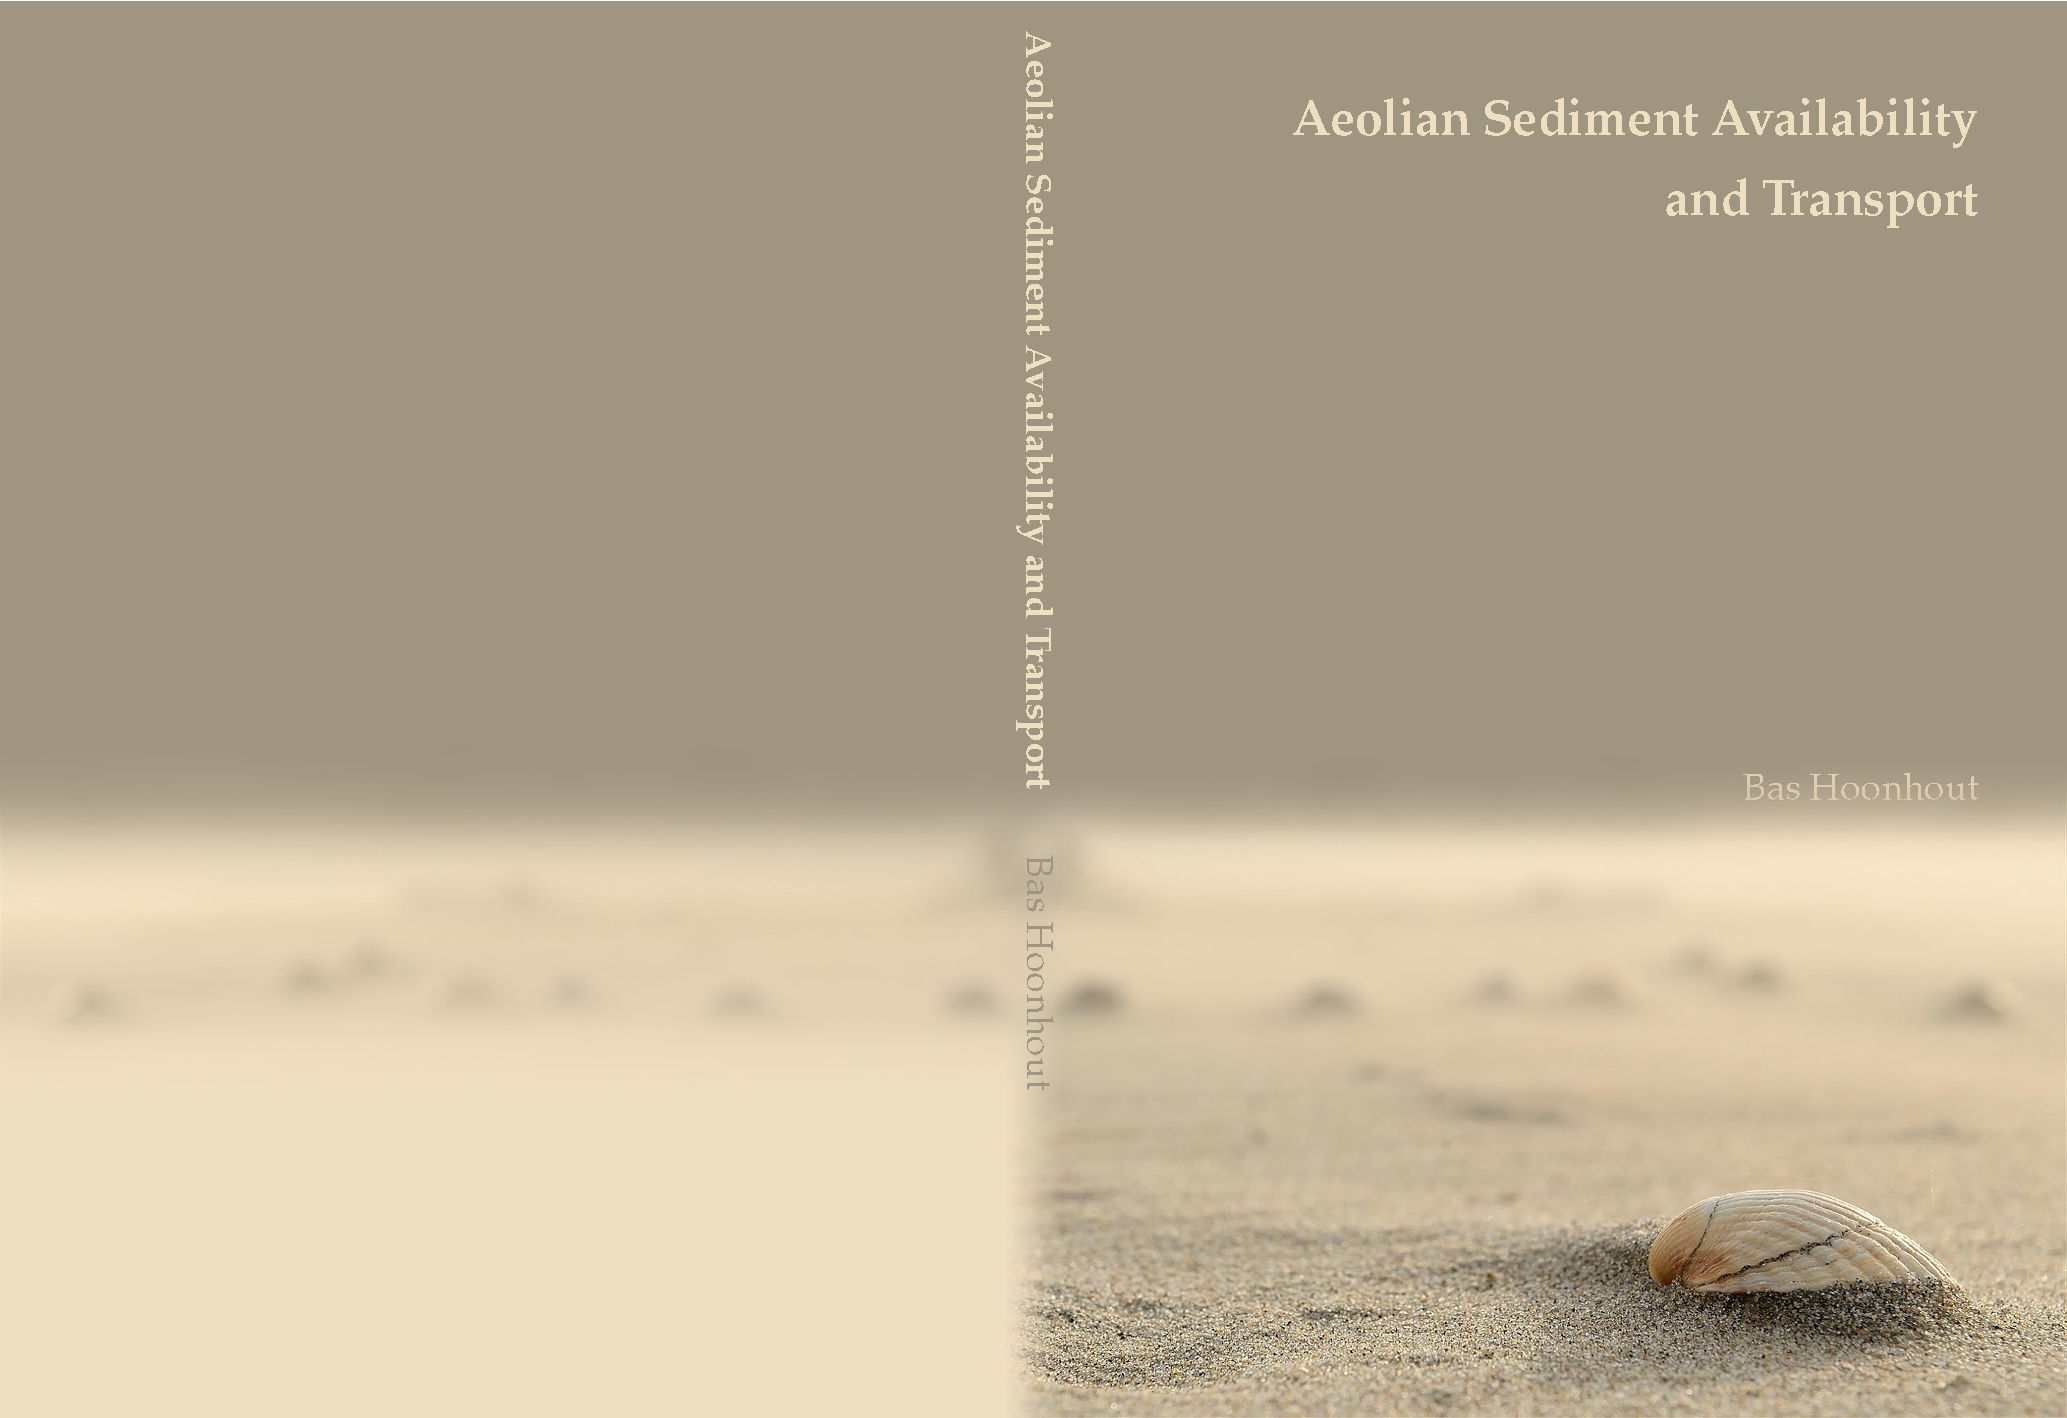
\includepdf[pages={1},
%              fitpaper=True,
%              % landscape=True,
%              link=True,
%              linkname=cover]{cover.pdf}
%  \cleardoublepage
%}

\begin{titlepage}
  \begin{center}
    \hfill
    
    \vspace{2cm}
    
    \begingroup
    \color{Maroon}\spacedallcaps{Aeolian Sediment Availability and Transport} \\ \bigskip
    \endgroup
    
    \spacedlowsmallcaps{Bas Hoonhout}
    
    \vfill
  \end{center}  
\end{titlepage}

%%% Local Variables:
%%% mode: latex
%%% TeX-master: "thesis"
%%% End:

\thispagestyle{empty}

\hfill

\vfill

\noindent Aeolian Sediment Availability and Transport \textcopyright\ 2016, Bas Hoonhout

%\bigskip

%\noindent Cover photo: Pulp Fiction \textcopyright\ 1994, Jules Winnfield

\bigskip

\noindent ISBN: XXX-XX-XXXX-XXX-X

%%% Local Variables:
%%% mode: latex
%%% TeX-master: "thesis"
%%% End:

\begin{titlepage}
  \begin{center}
    \hfill
    
    \vspace{2cm}
    
    \begingroup
    \color{Maroon}\spacedallcaps{Aeolian Sediment Availability and Transport} \\ \bigskip
    \endgroup
    
    \vfill
    
    \spacedallcaps{PROEFSCHRIFT}
    
    \vfill
    
    ter verkrijging van de graad van doctor \\
    aan de Technische Universiteit Delft, \\
    op gezag van de Rector Magnificus prof. ir. K.Ch.A.M. Luyben; \\
    voorzitter van het College voor Promoties, \\
    in het openbaar te verdedigen op \\
    vrijdag 24 maart 2017 om 12:30 uur.
    
    \vfill
    
    door
    
    \vfill
    
    Bastiaan Martin HOONHOUT \\
    civiel technisch ingenieur, TU Delft \\
    geboren te Amsterdam
    
    \vfill                      
    
  \end{center}  
\end{titlepage}

%%% Local Variables:
%%% mode: latex
%%% TeX-master: "thesis"
%%% End:

\thispagestyle{empty}

\hfill

\vfill

\noindent \spacedlowsmallcaps{Dit proefschrift is goedgekeurd door de promotor:}

\begin{table}[h]
  \begin{tabular}{l}
    Prof. dr. ir. M.J.F. Stive \\
  \end{tabular}
\end{table}

\noindent \spacedlowsmallcaps{Samenstelling promotie commissie:}

\begin{table}[h]
  \begin{tabular}{ll}
    Rector Magnificus          & Voorzitter \\
    Prof. dr. ir. M.J.F. Stive & Technische Universiteit Delft, Promotor \\
    Dr. ir. S. de Vries        & Technische Universiteit Delft \\
    \dots                      & \dots \\
    \dots                      & \dots \\
    \dots                      & \dots \\
  \end{tabular}
\end{table}

\vfill

\noindent Dr. ir. J. S. M. van Thiel de Vries en Dr. ir. S. de Vries
hebben als begeleider in belangrijke mate aan de totstandkoming van
het proefschrift bijgedragen.

\bigskip

%\noindent For the work discussed in this dissertation the author was
%supported by the ERC-Advanced Grant 291206 -- Nearshore Monitoring and
%Modeling (NEMO) and Deltares.
\noindent Het onderzoek ten behoeve van dit proefschrift is
gefinancieerd door de ERC-Advanced Grant 291206 -- Nearshore
Monitoring and Modeling (NEMO) en Deltares.

%%% Local Variables:
%%% mode: latex
%%% TeX-master: "thesis"
%%% End:

%\thispagestyle{empty}

\hfill

\vfill

\begin{flushright}
  
  \hangindent=15pt {\slshape All these years they worked like
    slaves. But they were happy in their work; they grudged no effort
    or sacrifice, well aware that everything that they did was for the
    benefit of themselves and those of their kind who would come after
    them, and not for a pack of idle, thieving human beings.}
  
  \medskip

  --- George Orwell in Animal Farm (1945)

\end{flushright}

\vfill

%%% Local Variables:
%%% mode: latex
%%% TeX-master: "thesis"
%%% End:


\frontmatter
\pdfbookmark[0]{Contents}{contents}
\setcounter{tocdepth}{2} % <-- 2 includes up to subsections in the ToC
\setcounter{secnumdepth}{3} % <-- 3 numbers up to subsubsections
\tableofcontents 

%%% Local Variables:
%%% mode: latex
%%% TeX-master: "thesis"
%%% End:

\pdfbookmark[0]{Definitions}{definitions}
\chapter*{Definitions}
\label{ch:definitions}

\begin{description}
\item[wind transport capacity] [$\mathrm{kg/m/s}$] Transport capacity
  of the wind over an idealized bed. The wind transport capacity is an
  upper limit of the (sediment) transport capacity that includes the
  influence of bed surface properties.
\item[(sediment) transport capacity] [$\mathrm{kg/m/s}$] Transport
  capacity of the wind over a given bed. The (sediment) transport
  capacity accounts for the impact velocity threshold. The (sediment)
  transport capacity is an upper limit of the actual sediment
  transport.
\item[equilibrium sediment transport] Sediment transport capacity.
\item[saturated sediment transport] Sediment transport capacity.
\item[velocity threshold] [$\mathrm{kg/m/s}$] Impact velocity
  threshold at which sediment transport is sustained over a given
  bed. The threshold depends on bed surface properties that may hamper
  saltation, e.g. roughness, moist, salt, and represents the
  difference between the wind and (sediment) transport capacity.
\item[sediment availability] [$\mathrm{kg/m^2}$] Sediment currently
  available for entrainment \citep[following ][]{Kocurek1999}. The
  sediment availability includes the fluid velocity threshold at which
  sediment transport is initiated. Sediment availability may result in
  sediment supply if wind is sufficient.
\item[sediment entrainment] [$\mathrm{kg/m^2/s}$] Entrainment of
  currently available sediment by the wind and contributing to the
  sediment supply.
\item[sediment supply] [$\mathrm{kg/m/s}$] Transport of entrained
  sediment from one location to another, e.g. from marine sources to
  intertidal beach or from intertidal beach to dunes.
\item[transport-limited] Transport is determined by the wind transport
  capacity. An increase in wind speed will result in an increase in
  sediment transport as long as sediment is still available. If
  insufficient sediment is available, the coastal system becomes
  availability-limited.
\item[availability-limited] Transport is determined by the
  availability of aeolian sediment. An increase in wind speed will not
  result in an increase in sediment transport as no additional
  sediment is available. A decrease in wind speed can result in a
  transport-limited coastal system as the sediment availability might
  be able to fulfill the demand from the reduced wind.
\item[supply-limited] Availability-limited.
\item[fetch-limited] Transport is determined by the available fetch
  and therefore a wider beach or more oblique wind will result in an
  increase in sediment transport. In this thesis fetch is only
  considered a limiting factor on an idealized bed with maximum
  sediment availability (i.e. flat, dry, loose and homogeneous). The
  coastal system is considered fetch-limited if and only if the
  available fetch is shorter than the fetch necessary for the
  development of a saturated saltation cascade in these idealized
  conditions. In all other cases where the available fetch influences
  the sediment transport, the coastal system is considered
  availability-limited.
\item[sediment sorting] Spatial sorting of (sandy) sediment, either
  horizontally or vertically, due to differences in (sediment)
  transport capacity between sediment fractions.
\item[beach armoring] Emergence of non-erodible roughness elements
  from the bed that shelter (sandy) sediment from wind erosion,
  resulting in spatiotemporal differences in sediment availability.
\end{description}

%%% TeX-master: "thesis"
%%% Local Variables: %%% mode: latex %%% TeX-master: "thesis" %%% End:

\pdfbookmark[0]{Acronyms}{acronyms}
\chapter*{acronyms}

\begingroup
\def\arraystretch{1.5}%  1 is the default, change whatever you need
\begin{tabular}{ll}
  \spacedlowsmallcaps{2DH} & Two-Dimensional in a Horizontal plane \\
  \spacedlowsmallcaps{2DV} & Two-Dimensional in a Vertical plane \\
  \spacedlowsmallcaps{ATV} & All-Terrain Vehicle \\
  \spacedlowsmallcaps{AeoLiS} & Aeolian sediment transport with Limited Supply \\
  \spacedlowsmallcaps{DN} & Deployment Number \\
  \spacedlowsmallcaps{KNMI} & Koninklijk Nederlands Meteorlogisch Instituut \\
  \spacedlowsmallcaps{MCMC} & Markov Chain Monte Carlo \\
  \spacedlowsmallcaps{MSL} & Mean Sea Level \\
  \spacedlowsmallcaps{MegaPEX} & Mega Peturbation EXperiment \\
  \spacedlowsmallcaps{NEMO} & Nearshore Modeling and Monitoring \\
  \spacedlowsmallcaps{$\mathrm{R^2}$} & R-squared or Coefficient of Determination \\
  \spacedlowsmallcaps{RMSE} & Root Mean Square Error \\
  \spacedlowsmallcaps{RTK-GPS} & Real-Time Kinematic Global Positioning System \\
\end{tabular}
\endgroup

%%% Local Variables:
%%% mode: latex
%%% TeX-master: "thesis"
%%% End:

\pdfbookmark[0]{Symbols}{symbols}
\chapter*{Symbols}
\label{ch:symbols}

\begin{longtable}{p{1cm} p{2cm} p{7.75cm}}
  Symbol & Units & Description \\
  \hline
  \endfirsthead
  Symbol & Units & Description \hfill (continued)\\
  \hline
  \endhead
  $\alpha$ & - & Factor to convert from wind velocity to shear velocity. \\
  $\beta$ & - & Ratio between drag coefficients of bare surface and roughness elements. \\
  $\theta_u$ & - & Wind direction. \\
  $\Gamma$ & - & Implicitness parameter. \\
  $\gamma$ & - & Maximum wave height over depth ratio. \\
  $\zeta$ & - & Bed interaction factor. \\
  $\eta$ & m+MSL & Still water level. \\
  $\hat{\eta}$ & m+MSL & Local water level. \\
  $\kappa$ & - & Von K{\'a}rm{\'a}n constant. \\
  $\lambda$ & - & Roughness density. \\
  $\xi$ & - & Surf similarity parameter. \\
  $\rho_{\mathrm{a}}$ & $\mathrm{kg/m^3}$ & Air density. \\
  $\rho_{\mathrm{p}}$ & $\mathrm{kg/m^3}$ & Grain density. \\
  $\rho_{\mathrm{w}}$ & $\mathrm{kg/m^3}$ & Water density. \\
  $\sigma$ & - & Ratio between surface area and frontal area of roughness elements. \\
  $\Phi$ & kg/m/s & Space-integrated entrainment function. \\
  $\phi$ & $\mathrm{kg/m^2/s}$ & Entrainment function. \\
  $\Psi$ & kg/s & Sediment transport potential. \\
  $A$ & - & Empirical coefficient. \\
  $A_{\mathrm{c}}$ & $\mathrm{m^2}$ & Surface area of control area. \\
  $C$ & - & Empirical coefficient to account for grain size distribution width. \\
  $C_{\mathrm{c}}$ & $\mathrm{kg/m^3}$ & Sediment concentration in the air as used by \citet{deVries2014a}. Relates to $c$ as $c = h C_{\mathrm{c}}$. \\
  $c$ & $\mathrm{kg/m^2}$ & Sediment concentration in the air. \\
  $c_{\mathrm{sat}}$ & $\mathrm{kg/m^2}$ & Saturated sediment concentration in the air. \\
  $D$ & $\mathrm{kg/m^2}$ & Total deposition. \\
  $D_{\mathrm{n}}$ & m & Reference median grain size (250 $\mu \mathrm{m}$). \\
  $d$ & m & Water depth. \\
  $d_{50}$ & m & Median grain size. \\
  $d_{\mathrm{n}}$ & m & Nominal grain size. \\
  $E$ & $\mathrm{kg/m^2}$ & Total erosion. \\
  $E_{\mathrm{v}}$ & m/s & Evaporation rate. \\
  $F$ & m & Available fetch. \\
  $\hat{F}$ & m & Effective fetch. \\
  $F_{\mathrm{c}}$ & m & Critical fetch.\\
  $f_{\Delta z_\mathrm{d}}$ & - & Depth of disturbance factor. \\
  $f_{\theta_u}$ & - & Factor to include wind direction in sediment transport capacity. \\
  $f_{u_\mathrm{* th},M}$ & - & Factor to include the influence of moisture to the shear velocity threshold $u_{\mathrm{* th}}$. \\
  $f_{u_\mathrm{* th},R}$ & - & Factor to include the influence of roughness elements to the shear velocity threshold $u_{\mathrm{* th}}$.  Relates to $R_{\mathrm{t}}$ as $R_{\mathrm{t}} = \frac{1}{f_{u_\mathrm{* th},R}}$. \\
  $f_{u_\mathrm{* th},S}$ & - & Factor to include the influence of salt to the shear velocity threshold $u_{\mathrm{* th}}$. \\
  $g$ & $\mathrm{m/s^2}$ & Gravitational constant. \\
  $H$ & m & Offshore wave height. \\
  $\hat{H}$ & m & Local wave height. \\
  $h$ & m & Height of saltation layer. \\
  $i$ & - & Cross-shore grid index. \\
  $j$ & - & Alongshore grid index. \\
  $K^{\mathrm{+}}$ & - & Hydrodynamic addition mask. \\
  $K^{\mathrm{\times}}$ & - & Hydrodynamic multiplication mask. \\
  $k$ & - & Grain size fraction index. \\
  $k_0$ & - & Index of smallest non-erodible grain size fraction. \\
  $l$ & - & Diagonal index. \\
  $m$ & - & Factor to account for difference between mean and maximum shear stress. \\
  $m_{\mathrm{a}}$ & $\mathrm{kg/m^2}$ & Sediment availability. \\
  $n$ & - & Time step index. \\
  $n_{\mathrm{k}}$ & - & Number of grain size fractions. \\
  $n_{\mathrm{pc}}$ & - & Number of counted particles. \\
  $n_{\mathrm{x}}$ & - & Number of grid cells in cross-shore direction. \\
  $n_{\mathrm{y}}$ & - & Number of grid cells in alongshore direction. \\
  $p$ & - & Porosity. \\
  $p_{\mathrm{g}}$ & kg/kg & Geotechnical mass content of water. \\
  $p_{\mathrm{s}}$ & mg/g & Salt content. \\
  $p_{\mathrm{V}}$ & $\mathrm{m^3/m^3}$ & Volumetric water content. \\
  $Q$ & $\mathrm{m^3}$ & Cumulative sediment transport capacity. \\
  $q$ & kg/m/s & Sediment transport rate. \\
  $q_{\mathrm{sat}}$ & kg/m/s & Saturated sediment transport rate. \\
  $R$ & m & Wave runup height. \\
  $R_{\mathrm{t}}$ & - & Ratio between velocity threshold on bare surface $u_{\mathrm{*th,S}}$ and on surface including roughness elements $u_{\mathrm{*th,R}}$. \\
  $S_k$ & - & Degree of saturation of grain size fraction $k$. \\
  $\hat{S}_k$ & - & Effective degree of saturation of grain size fraction $k$, including the bed interaction parameter $\zeta$. \\
  $T$ & s & Adaptation time scale in advection equation. \\
  $t$ & s & Time. \\
  $\Delta t^n$ & s & Size of time step $n$. \\
  $u_*$ & m/s & Shear velocity. \\
  $u_z$ & m/s & Wind velocity at height $z$. \\
  $u_{\mathrm{*th,R}}$ & m/s & Shear velocity threshold of surface including roughness elements. \\
  $u_{\mathrm{*th,S}}$ & m/s & Shear velocity threshold of bare surface. \\
  $u_{\mathrm{*th}}$ & m/s & Shear velocity threshold. \\
  $u_{\mathrm{th}}$ & m/s & Wind velocity threshold. \\
  $u_{z,x}$ & m/s & Wind velocity component in x-direction and at height $z$. \\
  $u_{z,y}$ & m/s & Wind velocity component in y-direction and at height $z$. \\
  $V$ & $\mathrm{m^3}$ & Sediment volume. \\
  $V_{\mathrm{40\%}}$ & $\mathrm{m^3}$ & Sediment volume normalized to 40\% porosity. \\
  $\Delta V^n$ & $\mathrm{m^3}$ & Change in sediment volume in time step $n$. \\
  $w_k$ & - & Weighting factor for grain size fraction $k$ in right-hand-side of the advection equation. \\
  $w_k^{\mathrm{air}}$ & - & Weighting factor for grain size fraction $k$ based on the grain size distribution in the air. \\
  $w_k^{\mathrm{bed}}$ & - & Weighting factor for grain size fraction $k$ based on the grain size distribution in the bed. \\
  $x$ & m & Cross-shore distance. \\
  $\Delta x_{i,j}$ & m & Size of grid cell $i,j$ in cross-shore direction. \\
  $y$ & m & Alongshore distance. \\
  $\Delta y_{i,j}$ & m & Size of grid cell $i,j$ in alongshore direction. \\
  $z$ & m & Height above the bed. \\
  $z'$ & m & Thickness of inner boundary layer. \\
  $z_{\mathrm{b}}$ & m+MSL & Bed level. \\
  $\Delta z_{\mathrm{d}}$ & m & Depth of disturbance. \\
\end{longtable}

%%% Local Variables:
%%% mode: latex
%%% TeX-master: "thesis"
%%% End:

\pdfbookmark[0]{List of Figures}{listoffigures}
\listoffigures
\pdfbookmark[0]{List of Tables}{listoftables}
\listoftables
\cleardoublepage
\pdfbookmark[0]{Abstract}{abstract}
\chapter*{Abstract}

This thesis explores the nature of aeolian sediment availability and
its influence on aeolian sediment transport with the aim to improve
large scale and long term aeolian sediment transport estimates in
(nourished) coastal environments. The generally poor performance of
aeolian sediment transport models in coastal environments is often
accredited to limitations in sediment availability. Sediment
availability can be limited by particular properties of the bed
surface. For example, if the beach is moist or covered with
non-erodible elements, like shells. If sediment availability is
limited, the aeolian sediment transport rate is governed by the
sediment availability rather than the wind transport capacity.

Aeolian sediment availability is rather intangible as sediment
availability is not only affected by aeolian processes, but also by
marine and meteorological processes that act on a variety of spatial
and temporal scales. The Sand Motor mega nourishment provides a unique
opportunity to quantify the spatiotemporal variations in aeolian
sediment availability and its effect on aeolian sediment
transport. Aeolian sediment accumulation in the Sand Motor region is
low compared to the wind transport capacity, while the Sand Motor
itself is virtually permanently exposed to wind and accommodates large
fetches. Aeolian sediment accumulation is therefore largely determined
by the sediment availability rather than the wind transport capacity.

Multi-annual bi-monthly measurements of the Sand Motor's topography
are used for a large scale aeolian sediment budget analysis. The
analysis revealed that aeolian sediment supply from the dry beach
area, that is permanently exposed to wind, diminished a half year
after construction of the Sand Motor in 2011 due to the development of
a beach armor layer. From early 2012, two-third of the aeolian
sediment deposits originate from the intertidal beach area. The source
of aeolian sediment in the Sand Motor region is remarkable as the
intertidal beach is periodically flooded and permanently moist.

The importance of the intertidal beach area in the Sand Motor region
is tested during a six-week field campaign. Gradients in aeolian
sediment transport are measured during the field campaign as to
localize aeolian sediment source and sink areas. A consistent supply
from the intertidal beach area was measured that was temporarily
deposited at the dry beach. The temporary deposits were transported
further during high water, when sediment supply from the intertidal
beach ceased, resulting in a continuous sediment supply to the
dunes. The temporary deposition of sediment at the dry beach was
likely promoted by the presence of a berm that affects the local wind
shear. Moreover, the berm edge coincided with the onset of the beach
armor layer that might have further promoted deposition of sediment.

The measurements on spatiotemporal variations in aeolian sediment
availability and supply inspired an attempt to capture the
characteristics of aeolian sediment availability in coastal
environments in a comprehensive model approach. The resulting model
simulates spatiotemporal variations in bed surface properties and
their combined influence on aeolian sediment availability and
transport. The implementation of multi-fraction aeolian sediment
transport in the model introduces the recurrence relation between
aeolian sediment availability and transport through self-grading of
sediment.

The model was applied in a four-year hindcast of the Sand Motor mega
nourishment as first attempt to field validation. The model reproduces
the multi-annual aeolian sediment erosion and deposition volumes, and
the relative importance of the intertidal beach area as source of
aeolian sediment well. Seasonal variations in aeolian sediment
transport are incidentally missed by the model. The model accuracy is
reflected in a $\mathrm{R^2}$ value of 0.93 when comparing time series
of measured and modeled total aeolian sediment transport volumes in
the four years since construction of the Sand Motor. The results
suggest that indeed significant limitations in sediment availability,
due to soil moisture content and beach armoring, govern aeolian
sediment transport in the Sand Motor region. A comparison with a
simulation without limitation in sediment availability suggests that
aeolian sediment availability in the Sand Motor region is limited to
about 25\% of the wind transport capacity. Moreover, both spatial and
temporal variations in aeolian sediment availability as well as the
recurrence relation between aeolian sediment availability and
transport are essential to accurate long term and large scale aeolian
sediment transport estimates.


%%% Local Variables:
%%% mode: latex
%%% TeX-master: "thesis"
%%% End:

\pdfbookmark[0]{Samenvatting}{samenvatting}
\begin{otherlanguage}{dutch}
\chapter*{Samenvatting}
Dit proefschrift onderzoekt de invloed van beschikbaarheid van eolish
sediment op eolisch sediment transport met als doel het verbeteren van
grootschalige en lange termijn voorspellingen van eolisch sediment
transport in (gesuppleerde) kustgebieden. Bestaande modellen voor
eolisch sediment transport presteren in het algemeen slecht in
kustgebieden. De slechte prestaties worden dikwijls geweten aan een
beperkte beschikbaarheid van eolisch sediment. De beschikbaarheid van
eolisch sediment kan worden beperkt door specifieke eigenschappen van
het strandoppervlak. Als bijvoorbeeld het strand vochtig is of bedekt
met niet-erodeerbare elementen, zoals schelpen, kan de beschikbaarheid
van sediment worden beperkt. In dat geval wordt de eolische sediment
flux bepaald door de beschikbaarheid van sediment in plaats van de
transportcapaciteit van de wind.

De beschikbaarheid van eolisch sediment is een redelijk ongrijpbaar
fenomeen, omdat deze niet alleen wordt be{\:i}nvloed door eolische
processen, maar ook door marine en meteorologische processen die op
verschillende ruimtelijke en temporele schalen actief zijn. De
Zandmotor megasuppletie biedt een unieke gelegenheid om de temporele
en ruimtelijke variaties in de beschikbaarheid van eolisch sediment en
het effect daarvan op eolisch sediment transport te
kwantificeren. Instuifvolumes rond de Zandmotor zijn klein in
vergelijking met de transportcapaciteit van de wind, terwijl de
Zandmotor met haar grote strijklengtes zelf vrijwel permanent
blootgesteld is aan wind. De instuiving van sediment wordt daar dus
grotendeels bepaald door de beschikbaarheid van sediment in plaats van
de transportcapaciteit van de wind.

Meerjarige tweemaandelijkse metingen van de topografie van de
Zandmotor zijn gebruikt voor een grootschalige eolische sediment
budget analyse. Uit de analyse bleek dat de aanvoer van eolisch
sediment vanaf het droge strand, dat permanent blootgesteld is aan de
wind, vanaf een half jaar na de aanleg van de Zandmotor in 2011 sterk
is verminderd als gevolg van het ontstaan van een schelpenlaag. Vanaf
het begin van 2012 is tweederde van het instuifvolume afkomstig uit
het intergetijdengebied. Deze bron van eolische sediment rond de
Zandmotor is opmerkelijk omdat het intergetijdenstrand periodiek
overstroomd en permanent vochtig is.

Het belang van het intergetijdengebied strand rond de Zandmotor wordt
bevestigd tijdens een zes weken durende veld campagne. Tijdens deze
campagne zijn gradi{\:e}nten in eolisch sediment transport gemeten de
bron van eolisch sediment te bepalen. De gemeten constante aanvoer
vanuit het intergetijdengebied bleek tijdelijk te sedimenteren op het
droge strand. Deze tijdelijke afzettingen werden tijdens hoogwater
verder getransporteerd wanneer de sediment aanvoer vanaf het
intergetijdenstrand stagneerde. Hierdoor ontstond een continue toevoer
van sediment naar de duinen. De tijdelijke afzetting van sediment op
het droge strand werd vermoedelijk bevorderd door de aanwezigheid van
een berm die de lokale schuifspanning van de wind
be{\:i}nvloedt. Bovendien viel de rand van de berm samen met het begin
van de schelpenlaag die het neerslaan van sediment mogelijk verder
bevorderd heeft.

De gemeten ruimtelijke en temporele variaties in de beschikbaarheid
van eolisch sediment hebben een poging ge{\:i}nspireerd om de
kenmerken van beschikbaarheid van eolisch sediment aan de kust te
vatten in een alomvattende model aanpak. Het resulterende model
simuleert variaties in tijd en ruimte van eigenschappen van het
strandoppervlak en hun gezamenlijke invloed op de beschikbaarheid en
transport van eolisch sediment. De implementatie van eolisch sediment
transport over meerdere korrelgrootte fracties in het model
introduceert de recurrente betrekking tussen de beschikbaarheid en het
transport van eolisch sediment door middel van zelfgradering van
sediment.

Het model is toegepast in een vierjarige hindcast van de Zandmotor
megasuppletie als eerste poging tot veldvalidatie. Het model
reproduceert de meerjarige erosie en depositie volumes van eolisch
sediment, en het relatieve belang van het intergetijdengebied als bron
van eolisch sediment, goed. Seizoensafhankelijke variaties in eolisch
sediment transport worden soms gemist door het model. De
nauwkeurigheid van het model is weerspiegeld in een $\mathrm{R^2}$
waarde van 0,93 wanneer gemeten en gemodelleerde tijdseries voor het
totaal door de wind getransporteerde sedimentvolume in de vier jaar na
constructie van de Zandmotor worden vergeleken. De resultaten
suggereren dat significante beperkingen in sediment beschikbaarheid,
als gevolg van het vochtgehalte van het strand en het vormen van een
schelpenlaag, inderdaad bepalend zijn voor het eolisch sediment
transport rond de Zandmotor. Een vergelijking met een simulatie zonder
beperking in beschikbaarheid van sediment suggereert dat de
beschikbaarheid van eolisch sediment rond de Zandmotor is beperkt tot
ongeveer 25\% van de transportcapaciteit van de wind. Bovendien zijn
zowel de ruimtelijke en temporele variaties in de beschikbaarheid van
eolisch sediment, evenals de recurrente betrekking tussen de
beschikbaarheid en transport van eolisch sediment essentieel voor een
nauwkeurige lange termijn en grootschalige voorspellingen van eolisch
sediment transport.
\end{otherlanguage}


%%% Local Variables:
%%% mode: latex
%%% TeX-master: "thesis"
%%% End:

\cleardoublepage

\mainmatter
\pagenumbering{arabic}

\chapter{Introduction} \label{ch:introduction}

\section{Motivation}

Aeolian sediment transport is a prerequisite to growth and resilience
of coastal dunes. Coastal dunes function as a natural protection
against flooding from the sea. As human societies are particularly
attracted to low-lying areas near the sea, the reliability and
resilience of the protective coastal dune systems becomes vital for
economic activities and human well-being. This societal demand for a
safe and comfortable living space, that initiated the discipline of
coastal engineering, developed our understanding of coastal safety
tremendously in the past decades. The increased understanding of our
coastal systems resulted in structural mitigation of coastal risks
using rigid solutions or local nourishments \citep{Hamm2002} and the
engineering of entire coastlines worldwide \citep{Donchyts2016}.

With the increased confidence in our ability to mitigate coastal
risks, additional demands and functions for coastal flood protections
arose. Soft engineering solutions with limited environmental and
ecological impact gained preference over rigid solutions. Recently,
the exponent of soft engineering emerged as nature-based coastal flood
protections \citep{Waterman2010, deVriend2015}. Nature-based flood
protections pursue the idea of stimulating natural processes with the
aim of increasing coastal safety and is based on the assumption that
the incidental or concentrated interventions necessary for the
stimulation of nature are less intrusive than classic solutions to
coastal safety. Moreover, nature-based solutions tend to accommodate
long-term monitoring and periodic adaptation and intervention that
increases flexibility with respect to planning and execution as well
as the occurrence of coastal hazards. The increased flexibility can
make nature-based flood protection also cost-effective
\citep{vanSlobbe2013}.

An innovative example of a nature-based solution to coastal safety is
the Sand Motor \citep[or Sand Engine,][]{Stive2013}. The Sand Motor is
an artificial sandy peninsula that was constructed along the Dutch
coast in 2011. The Sand Motor provides a 21 $\mathrm{Mm^3}$ sediment
source to the Dutch coast that is to be dispersed by natural
processes, like tides and waves, over a period of about two
decades. Although the construction of the Sand Motor clearly disturbs
the coastal system, the disturbance is incidental and concentrated. In
addition, the presence of the Sand Motor theoretically decreases the
necessity of measures to mitigate coastal risks at other locations
along the Dutch coast.

The Sand Motor is the provisional pinnacle of the evolution of soft
engineering solutions to coastal safety in The Netherlands. Soft
engineering solutions started with the dynamic preservation act of
1990 that prescribes extensive nourishment program initiated to
protect The Netherlands from flooding from the sea
\citep{MinVW1990b}. Since the start of the program the distance
between nourishments and dunes increased steadily. The initial dune
and beach nourishments were replaced by foreshore nourishments as
these are more cost-effective and less intrusive to the environmental
and recreational functions of the coastal dune system. Nature-based
solutions, like the Sand Motor, typically place nourishments
kilometers away from the dune system that needs to be enforced.

With the increasing distance between nourishments and dunes, the
effectiveness of nourishments in mitigating coastal risks becomes more
difficult to assess. Ultimately the reliability of coastal dune
systems is related to the sediment volume that is contained by the
system. However, also the location in the coastal profile where the
sediment resides is important. Sediment in the dunes provides a direct
buffer against flooding in case of storm erosion, while sediment on
the beach and foreshore influences coastal safety indirectly by
depth-induced breaking of waves and consequently a reduction of the
critical dune volume required to withstand a normative storm
\citep{Walstra2016}. The sediment volume that resides in the dunes
provides arguably a more persistent protection against flooding as the
volume is typically only affected by severe storms. In contrast, the
sediment volume that resides on the foreshore and beach is affected by
seasonal nearshore bar cycles and mild storms, which increase the
uncertainty of its contribution to coastal safety. It is therefore
relevant to understand how sediment arrives in the dunes and provide a
persistent contribution to coastal safety.

A key issue is to understand sediment transport pathways from
nourishment to dunes. Many studies and sophisticated numerical models
are available that describe hydrodynamic sediment transport. However,
only a small fraction of the sediment moved in the nearshore
ultimately arrives in the dunes \citep{Aagaard2004}. It is this small
wind-induced sediment flux that provides us with the natural and
persistent coastal flood protection that nature-based solutions aim
for. In addition, this small wind-induced sediment flux gives coastal
dune systems the natural resilience to storm impacts and the
conditions for survival of persistent dune vegetation that strengthens
the coastal dune systems, like marram grass \citep{Borsje2011}. It is
also this small wind-induced sediment flux that is least understood
and consistently overestimated by existing sediment transport models.

Aeolian sediment transport models describe the wind-induced sediment
transport rate. In coastal environments these models tend to
overestimate the aeolian sediment accumulation volumes, which is often
accredited to limitations in sediment availability \citep{Houser2009,
  DelgadoFernandez2012, deVries2014b}. Sediment availability can be
limited by particular properties of the bed surface. For example, if
the beach is moist or covered with non-erodible elements, like shells
\citep{Wiggs2004, Edwards2009, Namikas2010, McKennaNeuman2012}. If
sediment availability is limited, the aeolian sediment transport rate
is governed by the sediment availability rather than the wind
transport capacity, which violates the common assumption in aeolian
sediment transport models.

This thesis explores the nature of aeolian sediment availability and
its influence on aeolian sediment transport with the aim to improve
large scale and long term aeolian sediment transport estimates in
nourished coastal environments. This work is performed within the
framework of \emph{ERC-Advanced Grant 291206 -- Nearshore Monitoring
  and Modeling (NEMO)} that aims at an integrated modeling strategy
for large scale and long term coastal sediment transport that extends
from foreshore to backshore. Improving aeolian sediment transport
estimates helps the completion of the sediment transport pathways from
foreshore to backshore and from nourishment to dunes and thereby the
assessment of measures that attempt to mitigate coastal risks,
including nature-based coastal flood protections, on their
effectiveness.

%As much of the Sand Motor's behavior is difficult to
%predict with our current understanding of coastal systems, it should
%be seen as a large scale experiment and a unique opportunity to
%explore the characteristics of nature-based flood protections.

%The path of the righteous man is beset on all sides by the iniquities
%of the selfish and the tyranny of evil men. Blessed is he who in the
%name of charity and good will shepherds the weak through the valley of
%darkness, for he is truly his brother's keeper and the finder of lost
%children. And I will strike down upon thee with great vengeance and
%furious anger those who attempt to poison and destroy my brothers. And
%you will know my name is the Lord when I lay my vengeance upon thee.

\section{Research objectives}

This thesis pursues four main research objectives. Each chapter is
dedicated to one research objective. The research objectives are
elaborated in research questions that are addressed in the concluding
chapter of this thesis (Chapter \ref{ch:conclusions}). The research
objectives and questions are formulated as:

\begin{description}
\item[Research objective \#1] Identify the main sources for aeolian
  sediment in coastal environments and particularly at the Sand Motor
  mega nourishment (Chapter \ref{ch:largescale}).

  \medskip

  The research questions related to objective \#1 are:

  \begin{enumerate}[{1.}1]
%  \item \label{q:1.1} How can aeolian sediment fluxes be
%    separated from hydrodynamic sediment fluxes at the Sand Motor mega
%    nourishment?
  \item \label{q:1.2} What is the total aeolian sediment
    supply at the Sand Motor mega nourishment?
  \item \label{q:1.3} What are the main deposition areas of
    aeolian sediment at the Sand Motor mega nourishment?
  \item \label{q:1.4} What are the main source areas of
    aeolian sediment at the Sand Motor mega nourishment?
  \item \label{q:1.5} What bed surface characteristics can
    explain any spatial variations in aeolian sediment supply at the
    Sand Motor mega nourishment?
  \item \label{q:1.6} What is the relevance of these bed
    surface characteristics for coastal systems in general?
  \item \label{q:1.7} What characteristics of a coastal system
    determine aeolian sediment supply and dune growth?
  \end{enumerate}

  \bigskip

\item[Research objective \#2] Identify the main processes that govern
  aeolian sediment availability and supply in coastal environments and
  particularly at the Sand Motor mega nourishment (Chapter
  \ref{ch:smallscale}).

  \medskip

  The research questions related to objective \#2 are:

  \begin{enumerate}[{2.}1]
%  \item \label{q:2.1} How can aeolian sediment supply be measured in
%    the field?
  \item \label{q:2.2} What bed surface characteristics are related to
    aeolian sediment supply?
  \item \label{q:2.3} What processes govern the supply of aeolian
    sediment from the source areas?
  \item \label{q:2.4} What processes govern the deposition of aeolian
    sediment in the deposition areas?
  \end{enumerate}

  \bigskip

\item[Research objective \#3] Develop a numerical model approach to
  describe the influence of spatiotemporal variations in aeolian
  sediment availability on aeolian sediment transport and harmonize
  existing model approaches to aeolian sediment availability where
  possible (Chapter \ref{ch:model}).

  \medskip

  The research questions related to objective \#3 are:

  \begin{enumerate}[{3.}1]
  \item \label{q:3.1} What are existing model approaches to describe
    the influence of aeolian sediment availability on aeolian sediment
    transport, what are the similarities and differences among them
    and which approaches are mutually exclusive?
  \item \label{q:3.2} What processes that were identified to be
    relevant to aeolian sediment availability are not covered with
    sufficient accuracy by existing model approaches?
  \item \label{q:3.3} What are the requirements for a model approach
    that harmonizes existing, mutual inclusive model approaches and is
    conceptually able to describe all processes relevant to aeolian
    sediment availability and transport?
  \end{enumerate}

  \bigskip

\item[Research objective \#4] Validate the numerical model approach to
  reproduce the location and size of sources for aeolian sediment in
  coastal environments and particularly at the Sand Motor mega
  nourishment (Chapter \ref{ch:hindcast}).

  \medskip

  The research questions related to objective \#4 are:

  \begin{enumerate}[{4.}1]
  \item \label{q:4.1} Can the calibrated numerical model reproduce the
    total aeolian sediment supply at the Sand Motor mega nourishment
    with any statistical significance?
  \item \label{q:4.2} Can the calibrated numerical model reproduce the
    main source and deposition areas at the Sand Motor mega
    nourishment?
  %\item \label{q:4.3} Has the calibrated numerical model predictive
  %  capabilities?
  \item \label{q:4.4} What implemented processes are in retrospect
    significant to the model result?
  \end{enumerate}
\end{description}

\bigskip

\section{Thesis outline}

This thesis constitutes four parts:

\begin{enumerate}[{Part} I]
\item presents field data dedicated to the aeolian sediment supply and
  transport at the Sand Motor mega nourishment.

  Chapter \ref{ch:largescale} presents a large scale aeolian sediment
  budget analysis that identifies the main suppliers of aeolian
  sediment in the Sand Motor region.

  The large scale sediment budget analysis inspired the six-week field
  campaign presented in Chapter \ref{ch:smallscale}. Gradients in
  aeolian sediment transport were measured during the field
  campaign. Gradients in aeolian sediment transport reveal areas with
  net erosion and thereby the sources of aeolian sediment. The
  measurements therefore enable a detailed analysis of processes
  governing the spatiotemporal variations in aeolian sediment
  availability as identified in the aeolian sediment budget analysis.

\item presents a numerical model for aeolian sediment
  availability and transport that is inspired by the field
  observations.

  The field data show that significant spatial variations in aeolian
  sediment availability can exist and can affect net aeolian sediment
  transport rates. The variations in aeolian sediment availability
  coincide with changes in bed surface properties, like soil moisture
  content and beach armoring. In coastal environments these bed
  surface properties typically also vary in time. Assuming that the
  spatiotemporal variations in bed surface properties indeed influence
  the aeolian sediment availability and transport, a numerical aeolian
  sediment transport model is developed.

  Chapter \ref{ch:model} presents the model philosophy and design. The
  model focuses on the incorporation of spatiotemporal variability in
  aeolian sediment availability, which is illustrated using the
  process of beach armoring. Beach armoring occurs when roughness
  elements emerge from the bed and is a typical process that causes
  spatiotemporal variations in aeolian sediment availability. Both
  conceptual cases and wind tunnel experiments are used to illustrate
  the basic model behavior.

  Chapter \ref{ch:hindcast} describes the calibration and application
  of the model to the field data presented in Chapter
  \ref{ch:largescale} as a first attempt to field validation of the
  numerical model.

%In addition, the model is
%applied to data from the Sand Motor not presented in other chapters as
%to investigate the predictive capabilities of the model.

\item concludes this thesis by addressing the research objectives and
  questions, and a discussion on the nature of aeolian sediment
  availability and corresponding modeling strategies.

\item contains appendices with specifics on the reference model, the
  numerical model implementation and available model settings
  presented in Chapter \ref{ch:model}.

\end{enumerate}

%%% Local Variables:
%%% mode: latex
%%% TeX-master: "thesis"
%%% End:


\cleardoublepage
\ctparttext{Field data is collected at the Sand Motor mega nourishment
  in The Netherlands. The Sand Motor showed a peculiar morphological
  development since its construction as it is permanently exposed to
  wind and yet its sub-aerial morphology is remarkably static.
}
\part{Field data}

\chapter{Large scale sediment budgets}\label{ch:largescale}

\emph{This chapter is based on another publication: \bibentry{Hoonhout2017a}.}

\section{Introduction}

% context: intro nature-based flood defenses
Aeolian sediment supply is a prerequisite to growth and resilience of
coastal dunes that function as a natural protection against flooding
from the sea. Expanding human activities in coastal areas and growing
uncertainties related to climate change, increase coastal
risks. Mitigation of these risks resulted in the engineering of entire
coastlines \citep{Donchyts2016}. Rigid solutions and local
nourishments are traditional solutions to a societal demand for
coastal safety \citep{Hamm2002}. With the increased confidence in our
ability to mitigate coastal risks, additional demands and functions
for coastal flood protections arose. Soft engineering solutions with
limited environmental and ecological impact \citep{Waterman2010,
  deVriend2015} gained preference over rigid solutions or local
nourishments. Recently, the exponent of soft engineering emerged as
mega nourishments \citep{Stive2013}.  Mega nourishments pursue the
idea of stimulating natural sediment transport processes with the aim
of increasing coastal safety. The idea is based on the assumption that
the incidental or concentrated interventions necessary for the
stimulation of nature are less intrusive than classic solutions to
coastal safety. Moreover, mega nourishments tend to accommodate
long-term monitoring and periodic adaptation and intervention that
increases flexibility with respect to planning and execution as well
as the occurrence of coastal hazards. The increased flexibility can
make mega nourishments also cost-effective \citep{vanSlobbe2013}.

% context: role of aeolian sediment supply in nature-based flood defenses
The effectiveness of a mega nourishment depends on the sediment
transport pathways from nourishment to dunes. A small fraction of the
sediment moved in the nearshore ultimately arrives in the dunes
\citep{Aagaard2004}. It is this small aeolian sediment supply that
provides us with the natural and persistent coastal safety that mega
nourishments aim for. In addition, this small aeolian sediment supply
gives coastal dune systems the natural resilience to storm impacts and
the conditions for survival of persistent dune vegetation that
strengthens the dunes, like marram grass \citep{Borsje2011}. It is
also this small aeolian sediment supply that is least understood.

% what has been done?
Mega nourishments affect aeolian sediment supply to coastal dunes in
various ways. First, sand used for nourishment is typically obtained
from offshore borrowing pits and differs from the original beach sand
in terms of size and composition, affecting the erodibility of the
beach \citep{VanDerWal1998, VanDerWal2000}. Second, aeolian sediment
availability \citep[following the definition of][]{Kocurek1999} at
beach nourishments that are constructed above storm surge level can be
significantly reduced by deflation lag deposits
\citep{Jackson2010}. The absence of regular flooding and
wave-reworking allows lag deposits to develop a beach armor layer,
resulting in compartmentalization of the nourishment in armored and
unarmored surfaces. \citet{McKennaNeuman2012} illustrated how
deflation lag deposits increase the shear velocity threshold
significantly and reduce aeolian sediment availability and
subsequently supply from the higher supratidal beach. Deflation lag
deposits can therefore cause intertidal and low-lying supratidal
beaches to gain importance over the high and dry beach as source of
aeolian sediment. Third, the placement of a nourishment is known to
affect nearshore processes \citep{Grunnet2005, Ojeda2008,
  deSchipper2013}.  Synchronization between aeolian and nearshore
processes, like onshore bar migration and welding, is reported to
stimulate aeolian sediment supply to coastal dunes \citep{Houser2009,
  Anthony2013}. The importance of low-lying beaches as source of
aeolian sediment might therefore also be affected by changing bar
dynamics.
% , resulting in a complex morphological interplay between nourishment
% and aeolian sediment supply.

%\citep{Jackson1999, DavidsonArnott2005,
%  DavidsonArnott2008, Bauer2009}. Fetch is important as a certain
%distance is required for the development of a saturated saltation
%cascade. Because the saltation cascade develops slower when sediment
%is scarce, the critical fetch is inversely proportional to the
%sediment availability \citep{DelgadoFernandez2010}. In coastal
%environments the available fetch is often limited and depends on, for
%example, the wind direction. If the available fetch is shorter than
%the critical fetch, the wind transport capacity is not a reliable
%indicator for the actual sediment flux \citep{Bauer2002}
%
%

%Jackson2010
%measurements, models
%small nourishments
%short time scales
%nourishment strategies
%quantification
%dynamic

% what do we need?
\citet{Jackson2011} emphasized the necessity for the quantification of
the effect of large scale beach nourishment designs on aeolian
sediment supply. Quantitative predictions of aeolian sediment
availability and supply in coastal environments has proven to be
challenging \citep{Sherman1998, Sherman2012}. Limitations in aeolian
sediment availability are often identified as reason for the
discrepancy between measured and predicted sediment transport rates
\citep{DelgadoFernandez2012, deVries2014b, Lynch2016}.

Mega nourishments inherently cause spatiotemporal variations in
aeolian sediment availability. The spatial variations are caused by
compartmentalization of the beach. The temporal variations are induced
by adaptation of the large coastal disturbance to the wave and wind
climate, resulting in changing in beach width, slope and composition
\citep{deSchipper2016}. Consequently, quantification of aeolian
sediment availability and supply from mega nourishments requires
differentiation in space and time.

% what did we do?
This paper presents an aeolian sediment budget analysis of the 21
$\mathrm{Mm^3}$ Sand Motor mega nourishment based on four years of
bi-monthly topographic surveys. The sediment budget analysis
quantifies the net aeolian sediment supply to the dunes, dune lake and
lagoon accommodated by the Sand Motor. The Sand Motor constitutes
distinct areas that are either influenced by marine processes, by
aeolian processes or by a combination of both. Therefore, the
influence of marine and aeolian processes on aeolian sediment supply
can be separated and spatiotemporal variations in aeolian sediment
availability can be identified with reasonable accuracy. The observed
compartmentalization of the Sand Motor is discussed in relation to
limitations in aeolian sediment availability, as well as the design of
mega nourishments like the Sand Motor as solution to coastal safety.

%evaluation of mega-nourishment sand motor wrt ordinary nourishment as natural supplier of aeolian sediment
%role of dune lake and lagoon
%long-term aeolian sediment budget analysis
%identifies source and deposition area
%quantifies aeolian sediment supply
%lessons learned for mega nourishments


%% context
%The wind transport capacity is a poor indicator for the actual aeolian
%sediment transport rate in coastal environments \citep{Sherman1998,
%  Sherman2012}. Limitations in sediment availability \citep[following
%the definition of][]{Kocurek1999} are often identified as reason for
%the discrepancy between measured sediment transport rates and the wind
%transport capacity \citep[e.g.][]{Houser2009, DelgadoFernandez2012,
%  deVries2014b}. The sediment availability can be limited by a variety
%of bed surface properties; for example soil moisture is known to limit
%the sediment availability significantly \citep{Wiggs2004, Edwards2009,
%  Namikas2010}. An example of an availability-limited coastal system
%is the Sand Motor mega nourishment \citep[or Sand
%Engine;][]{Stive2013} where aeolian sediment transport rates only
%reach to about 25\% of the estimated wind transport
%capacity. Moreover, the Sand Motor accommodates a large spatial
%variation in bed surface properties and therefore provides a unique
%opportunity to investigate the influence of bed surface properties on
%coastal aeolian sediment transport and dune growth.
%
%% what has been done?
%Although consensus may exist that limitations in sediment availability
%are important for coastal aeolian sediment transport, it is still
%being debated how sediment availability influences aeolian sediment
%transport and how this influence can be measured best. Measurements on
%the influence of bed surface properties on the sediment availability
%date from the 1930's with the pioneering work of \citet{Bagnold1937b}
%and gained significant interest from the 1960's onward
%\citep[e.g.][]{Belly1964, Howard1977, Dyer1986, Gillette1989}. Studies
%on specific bed surface properties are typically performed in a wind
%tunnel and define an adapted threshold velocity that relates the
%theoretical wind transport capacity to a measured sediment transport
%capacity. In the new millennium an increasing number of field
%measurements is dedicated to the influence of sediment availability on
%aeolian sediment transport in coastal environments. Field measurements
%are typically performed in an attempt to find a distance at which
%saturated transport is reached: the critical fetch \citep{Jackson1999,
%  DavidsonArnott2005, DavidsonArnott2008, Bauer2009}. Fetch is
%important as a certain distance is required for the development of a
%saturated saltation cascade. Because the saltation cascade develops
%slower when sediment is scarce, the critical fetch is inversely
%proportional to the sediment availability
%\citep{DelgadoFernandez2010}. In coastal environments the available
%fetch is often limited and depends on, for example, the wind
%direction. If the available fetch is shorter than the critical fetch,
%the wind transport capacity is not a reliable indicator for the actual
%sediment flux \citep{Bauer2002}. As the critical fetch is relatively
%easy to measure, the critical fetch concept provides a convenient
%framework for field measurements. However, measurements on the
%critical fetch assume that, in case of sufficient fetch, saturated
%transport will be reached. In a truly availability-limited system this
%assumption is not necessarily valid: an increasing wind transport
%capacity or fetch will not lead to an increase in transport if no
%additional sediment is available. The subtle difference is especially
%important for nourished coasts for which sand is extracted from
%offshore borrowing pits.\mrq[ls]{1.6} Such coasts tend to contain many
%shells, shell fragments and other roughness elements that cause a
%significant limitation and spatiotemporal variability in sediment
%availability \citep{VanDerWal1998, VanDerWal2000,
%  McKennaNeuman2012}. When sediment availability is severely limited
%and is varying spatially, the critical fetch may become very large,
%highly variable or even undefined, which makes the definition and
%interpretation of the critical fetch impractical
%\citep{Lynch2016}. Recently, \citet{deVries2014a} proposed an
%alternative conceptual approach that is based on an explicit
%definition of sediment availability. This approach makes the
%assumption that saturated sediment transport is reached, given
%sufficient fetch, unnecessary. % \citet{Hoonhout2016} continue on this
%% approach by defining the sediment availability in terms of
%% (measurable) bed surface properties, like grain size, roughness
%% density and moisture content.
%
%% what do we need?
%% The explicit relation between bed surface properties and sediment
%% availability proposed by \citet{Hoonhout2016} provides a framework in
%% which the influence of arbitrary configurations of bed surface
%% properties on aeolian sediment availability and transport can be
%% described.
%Aeolian sediment availability or supply can be quantified explicitly
%in the field by a sediment budget analysis. A sediment budget analysis
%compares changes in sediment volumes between different pre-defined
%control areas. The control areas are defined such that homogeneous bed
%surface properties and sediment availability can be assumed within
%each control area. The analysis therefore provides insight in the
%relation between bed surface properties, sediment availability and
%supply. A major advantage of this approach is that regular topographic
%measurements can be used to directly measure the influence of sediment
%availability on aeolian sediment transport, even in complex coastal
%environments.
%
%% what did we do?
%This paper presents an extensive aeolian sediment budget analysis of
%the Sand Motor based on four years of bi-monthly topographic surveys
%\citep{deSchipper2016}. The sediment budget analysis localizes and
%quantifies spatial variations in sediment supply in the Sand Motor
%region. Despite the uniqueness of the Sand Motor, the properties and
%processes limiting aeolian sediment transport and dune growth are
%common and relevant for (nourished) beaches worldwide.

\section{Field Site}
\label{sec:fieldsite}

The Sand Motor (or Sand Engine) is an artificial 21 $\mathrm{Mm^3}$
sandy peninsula protruding into the North Sea off the Delfland coast
in The Netherlands \citep[Figure \ref{fig:fieldsite},][]{Stive2013}.
The Sand Motor is an example of a mega nourishment and is intended to
nourish the Holland coast for a period of two decades, while
stimulating both biodiversity and recreation.

\begin{figure}
  \centering
  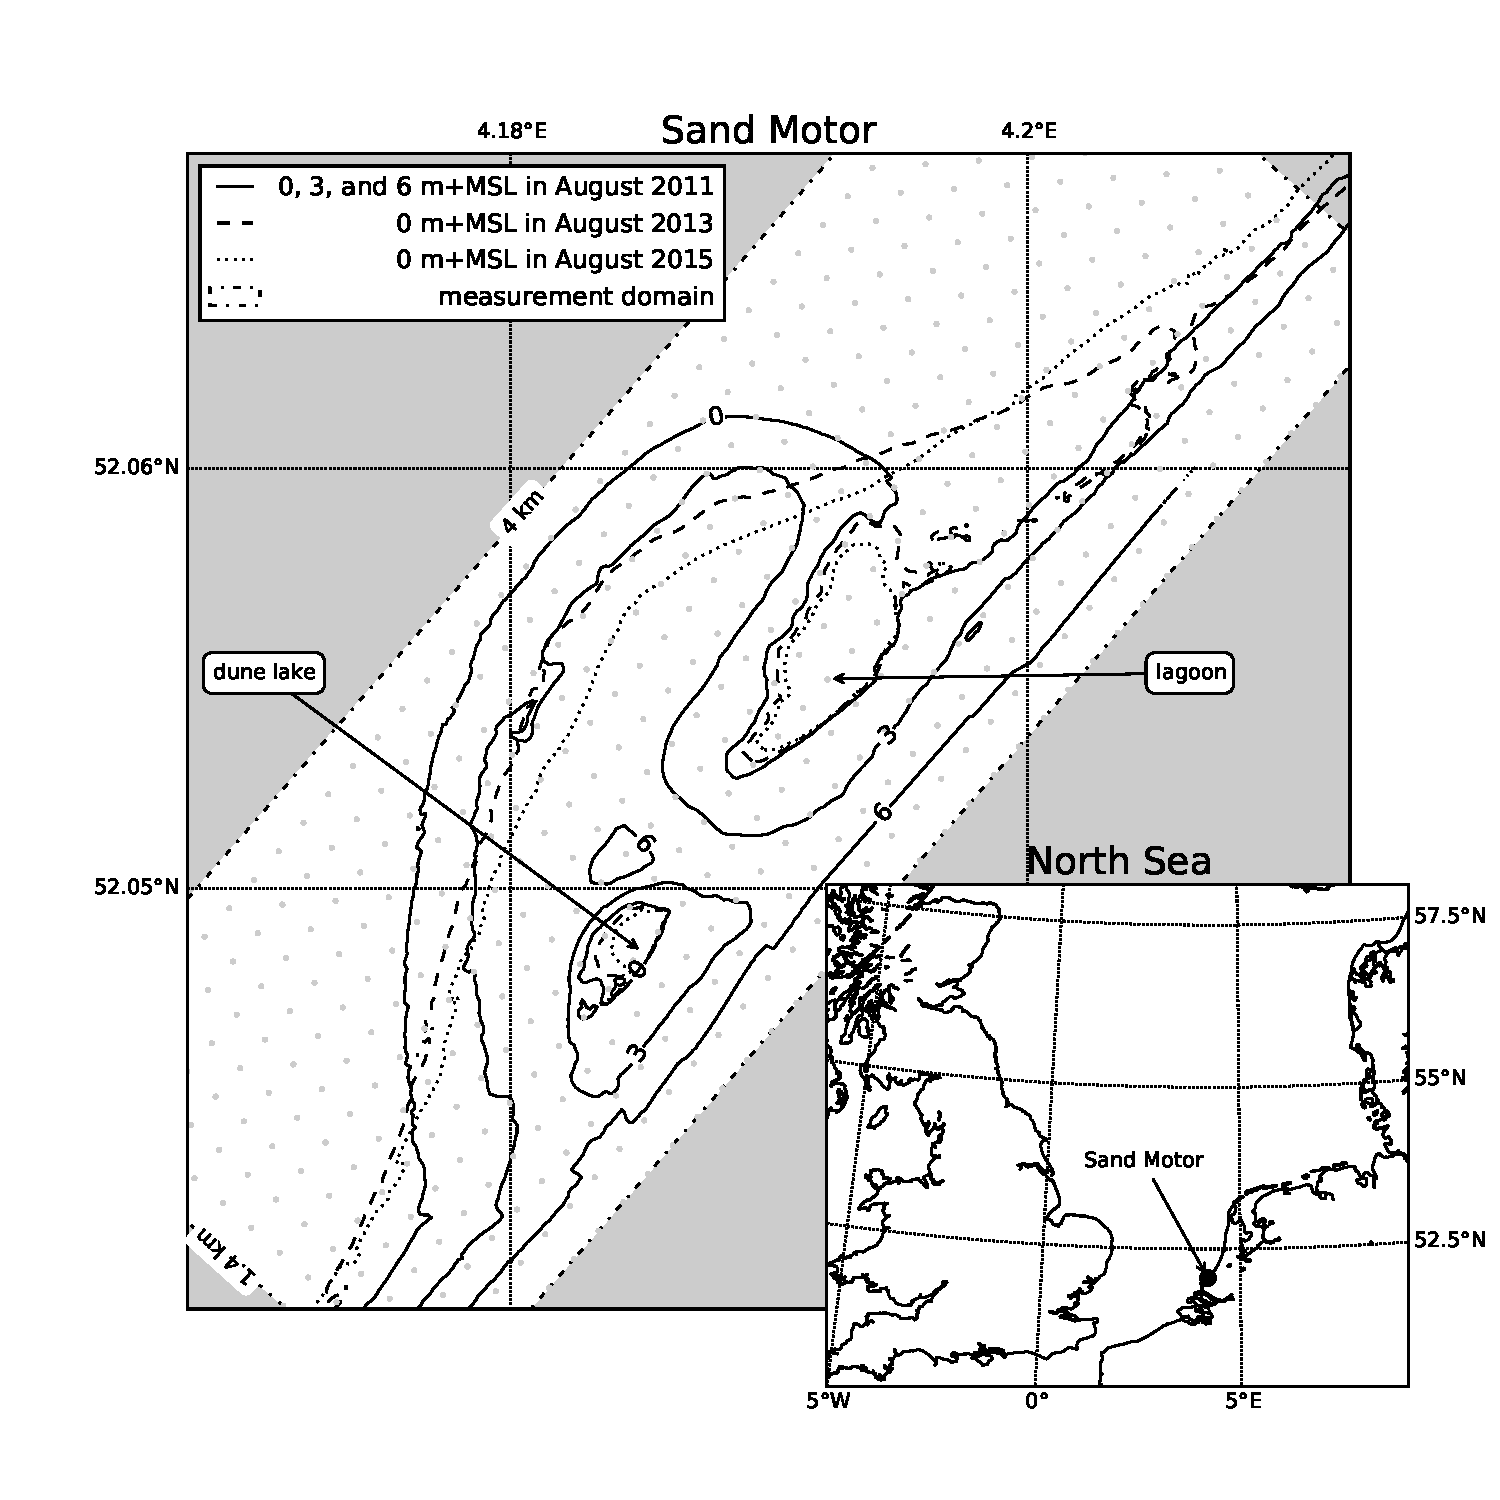
\includegraphics[width=\columnwidth]{../Figures/location_and_evolution}
  \caption{Location, orientation, appearance and evolution of the Sand
    Motor between construction in 2011 and 2015. The box indicates the
    measurement domain used in the remainder of this paper. A 100 x
    100 m grid aligned with the measurement domain is plotted in gray
    as reference.}
  \label{fig:fieldsite}
\end{figure}

The Sand Motor was constructed in 2011 and its bulged shoreline
initially extended about 1 km seaward and stretched over approximately
2 km along the original coastline. The original coast was
characterized by an alongshore uniform profile with a vegetated dune
with an average height of 13 m and a linear beach with a 1:40
slope. The dune foot is located at a height of approximately 5 m+MSL.

Due to natural sediment dynamics the Sand Motor distributes about 1
$\mathrm{Mm^3}$ of sand per year to the adjacent coasts (Figure
\ref{fig:fieldsite}). The majority of this sand volume is transported
by tides and waves. However, the Sand Motor is constructed up to 5
m+MSL and locally up to 7 m+MSL, which is in either case well above
the maximum surge level of 3 m+MSL (Figure
\ref{fig:windwaves}c). Therefore, the majority of the Sand Motor area
is uniquely shaped by wind.

The Sand Motor comprises both a dune lake and a lagoon that act as
large traps for aeolian sediment (Figure \ref{fig:fieldsite}). The
lagoon is affected by tidal forcing, although the tidal amplitude
quickly diminished over time as the entry channel elongated. The tidal
range of about 2 m that is present at the Sand Motor periphery (Figure
\ref{fig:windwaves}c), is nowadays damped to less than 20 cm inside
the lagoon \citep{deVries2015}. Consequently, the tidal currents at
the closed end of the lagoon, where most aeolian sediment is trapped,
are negligible.

Sand used for construction of the Sand Motor is obtained from an
offshore borrowing pit in the North Sea. The sand is predominantly
Holocene sand with a significant amount of fines. The median grain
size is slightly coarser than found originally along the Delfland
coast. Apart from sand fractions, the sediment contains a large amount
of shells, shell fractions, some pebbles and cobbles and an occasional
fraction of a mammoth bone.

%\begin{figure}
%  \centering
%  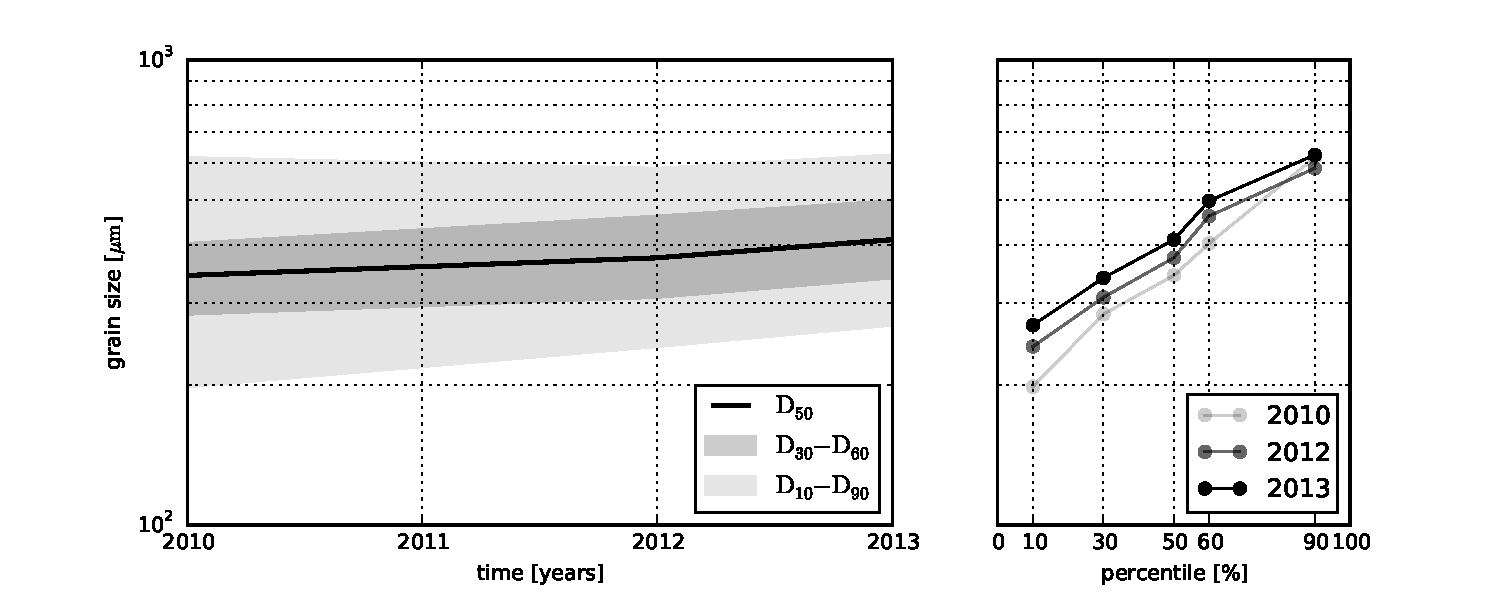
\includegraphics[width=\columnwidth]{../Figures/grainsize}
%  \caption{Evolution of the grain size distribution at the dry beach
%    since 2010, prior to construction of the Sand Motor
%    \citep{ImaresSamples}. Left panel: time series of median grain
%    size. Right panel: grain size distributions.}
%  \label{fig:grainsize}
%\end{figure}

The dominant wind direction at the Sand Motor is south to southwest
(Figure \ref{fig:windwaves}a). However, during storm conditions the
wind direction tends to be southwest to northwest. During extreme
storm conditions the wind direction tends to be
northwest. Northwesterly storms are typically accompanied by
significant surges as the fetch is virtually unbounded to the
northwest, while surges from the southwest are limited due to the
presence of the narrowing of the North Sea at the Strait of Dover
(Figure \ref{fig:fieldsite}, inset).

\begin{figure}
  \centering
  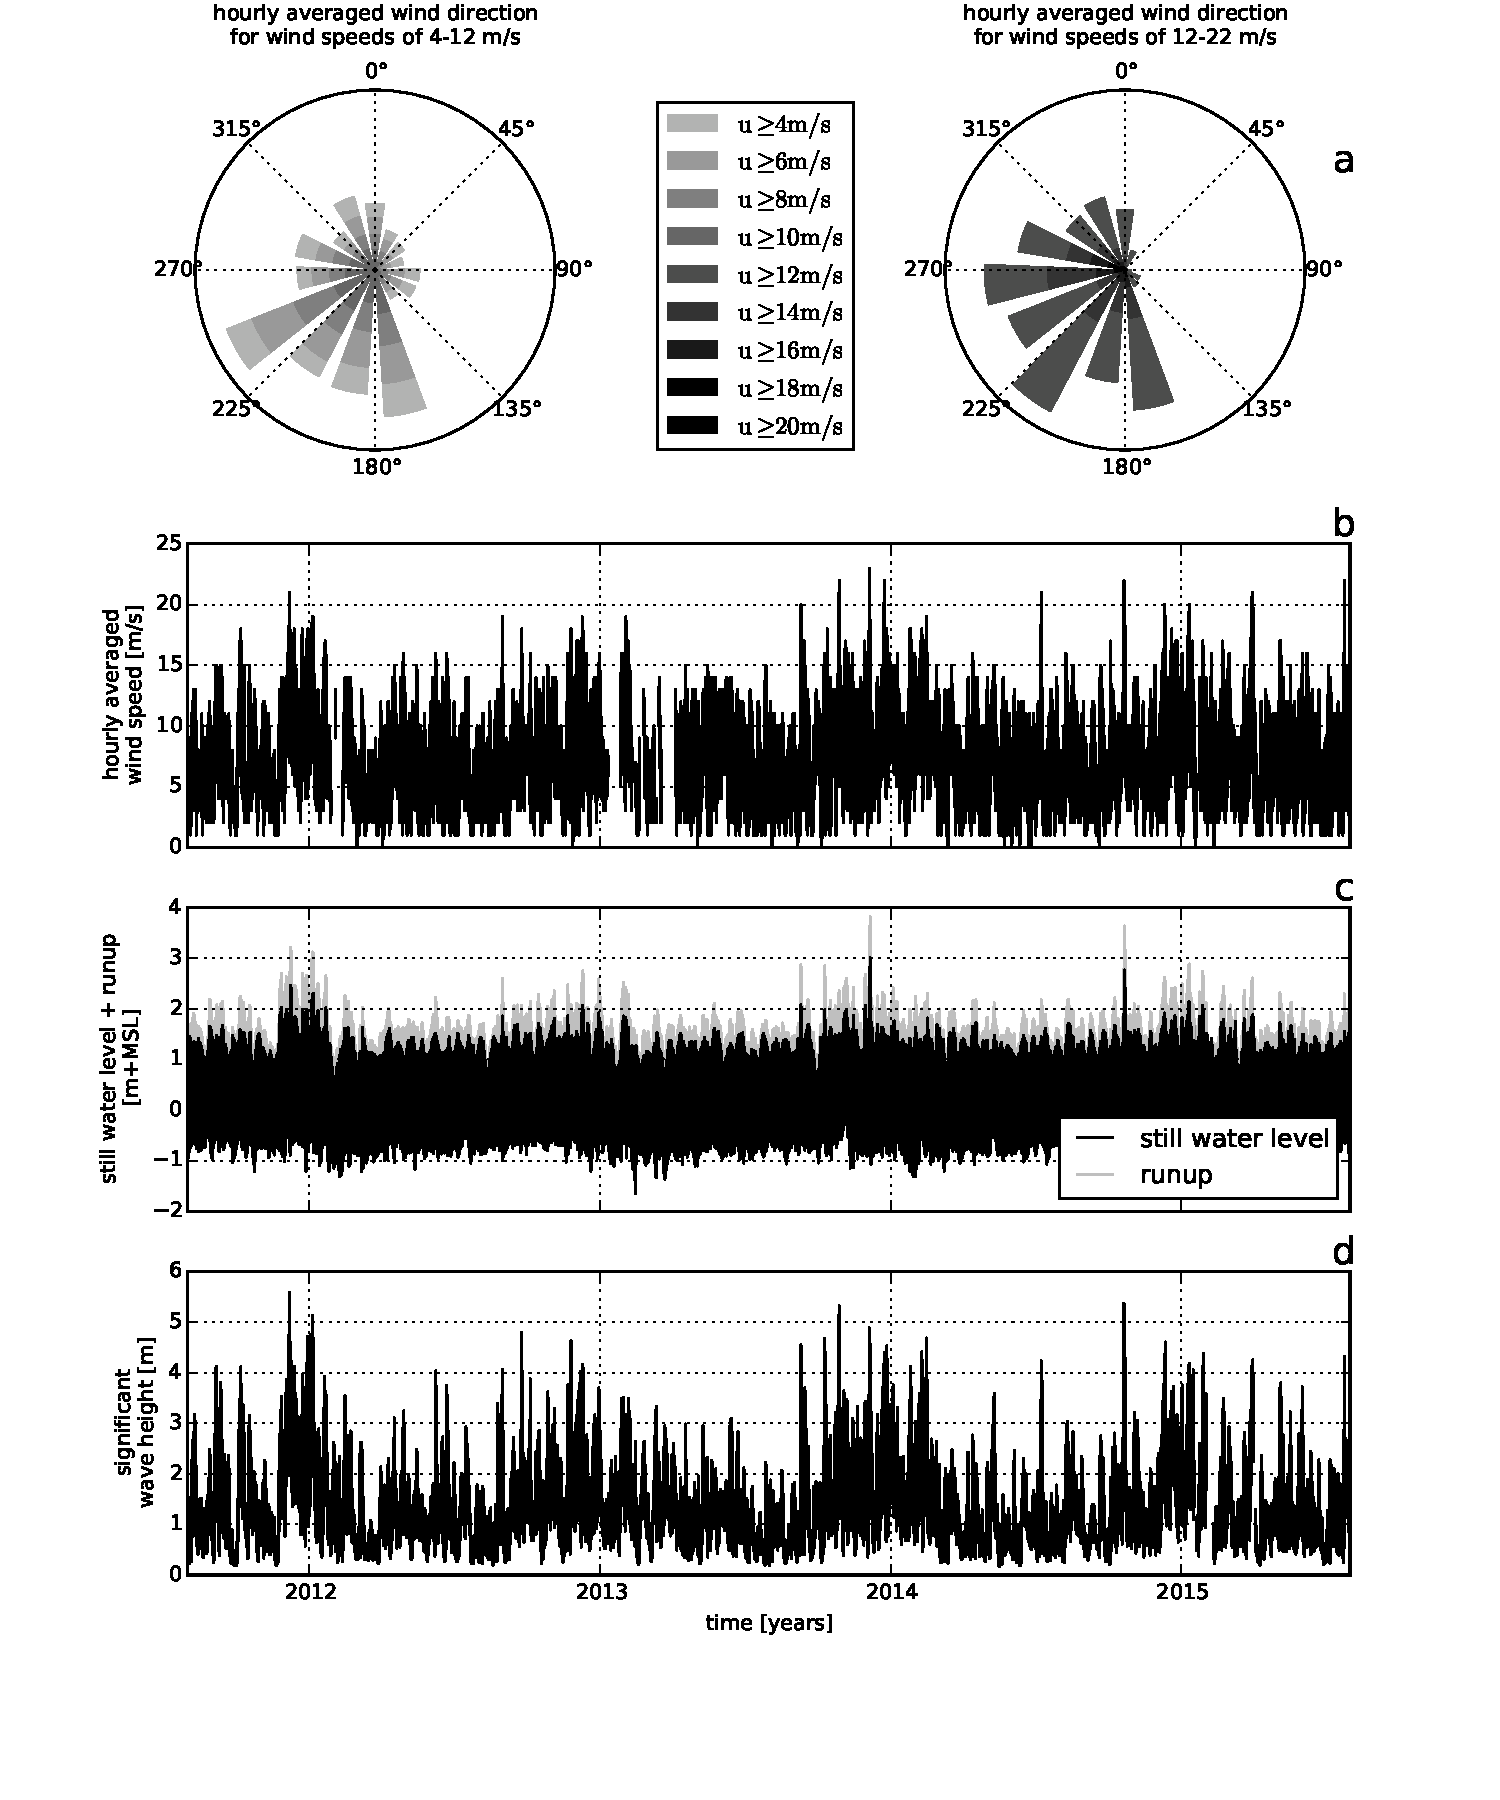
\includegraphics[width=\columnwidth]{../Figures/boundaryconditions}
  \caption{Wind and hydrodynamic time series from 2011 to 2015. Hourly
    averaged wind speeds and directions are obtained from the KNMI
    meteorological station in Hoek van Holland (upper
    panels). Offshore still water levels, wave heights and wave
    periods are obtained from the Europlatform (lower panels). Runup
    levels are estimated following \citet{Stockdon2006}.}
  \label{fig:windwaves}
\end{figure}

%The 21 $\mathrm{Mm^3}$ Sand Motor mega nourishment provides a unique
%opportunity to investigate the relation between bed surface
%properties, spatiotemporal variations in sediment availability, supply
%and aeolian sediment transport. At the Sand Motor, limitations in
%fetch are negligible as fetches can exceed 1.0 km depending on the
%location and wind direction. In addition, the Sand Motor accommodates
%a large spatiotemporal variability in bed surface properties:
%expanding moist intertidal beaches, pronounced intertidal bar dynamics
%and vast dry areas that are severely armored by the emergence of
%shells, shell fragments and other roughness elements that are
%contained by the sand from offshore borrowing pits. 

\section{Methodology}

Spatiotemporal variations in aeolian sediment supply in the Sand Motor
domain are identified using an aeolian sediment budget analysis. A
sediment budget analysis can be performed if frequent topographic
measurements are available \citep{DavidsonArnott1990} and sediment
exchange over the border of the measurement domain is limited. In a
sediment budget analysis the morphological change in predetermined
areas are converted to volumetric changes (budgets) that are compared
in a sediment volume balance.

A sediment budget analysis is particularly suitable for coastal sites
with a complex and dynamic topography, like the Sand Motor. The use of
(dense) topographic measurements ensures that any local variations in
the topography are included. Moreover, no assumptions on the local
representativeness of the measurements are needed and the methodology
is applicable to a wide range of spatial or temporal scales.

In the Sand Motor domain it is possible to separate the marine and
aeolian influence on erosion and deposition of sediment directly from
a sediment budget analysis. The high construction height of the Sand
Motor and the absence of regular storm surges in the first four years
after construction make that distinct areas exist that are either
influenced by marine or aeolian processes. The sediment budgets are
determined along the borders of these marine and aeolian zones.

%An aeolian sediment budget analysis has several advantages with
%respect to traditional measurements techniques, like sediment traps or
%saltation measurements, for the purpose of quantification of
%multi-annual aeolian sediment supply. Multi-annual deployment of
%sediment traps or saltation measurements in the Sand Motor domain is
%complicated by:
%
%
%\begin{enumerate}
%\item A complex, non-uniform topography that would require a large
%  number of measurement locations to account for the spatial variation
%  in aeolian sediment transport;
%\item A dynamic topography that would require constant relocation and
%  maintenance of instrumentation to prevent blocking, clogging or loss
%  of the instrumentation;
%\item The public accessibility of the area that would require constant
%  monitoring of instrumentation to prevent the measurements being
%  compromised;
%\item The necessity to translate trapped sediment volumes and/or
%  saltation rates to large scale sediment volumes, which would require
%  more extensive assumptions on the local representativeness of the
%  data than required in a sediment budget analysis.
%\end{enumerate}

\subsection{Topographic measurements}

32 topographic measurements of the Sand Motor domain obtained over a
period of four years are used to determine the overall sediment budget
of the Sand Motor domain \citep{deSchipper2016}. The measurement area
covers 1.4 km cross-shore and 4 km alongshore (Figure
\ref{fig:fieldsite}). The nearshore bathymetry is surveyed using a
jetski equipped with an echo sounder and RTK-GPS receiver. The
topography of the Sand Motor from the waterline up to the dune foot is
surveyed using an all-terrain vehicle (ATV) that is also equipped with
a RTK-GPS receiver. Inundated areas that are too shallow for the
jetski, like the tidal channel and the dune lake, are surveyed using a
manually pushed RTK-GPS wheel. The survey is performed along
cross-shore transects that are 20 m apart. The resulting trajectories
are interpolated to a regular 10 m x 10 m grid for the sediment budget
analysis. Surveys that show a morphological rate of change that is
more than two standard deviations from the average are considered
outliers. The measurements of September 4, 2011 and June 21, 2012 are
discarded as outliers.

The topography in the dune area, which is not included in the RTK-GPS
surveys, is monitored by airborne lidar. Half-yearly measurements from
the southern Holland coast (Delfland coast) are available since 2011,
prior to the construction of the Sand Motor. The lidar measurements
have a spatial resolution of 2 m or 5 m. The measurements are
corrected for the presence of vegetation and artificial objects, like
beach pavilions, and interpolated to the same 10 m x 10 m grid and the
same moments in time as the RTK-GPS measurements.

\subsection{Zonation}
\label{sec:zonation}

\begin{figure}
  \centering
  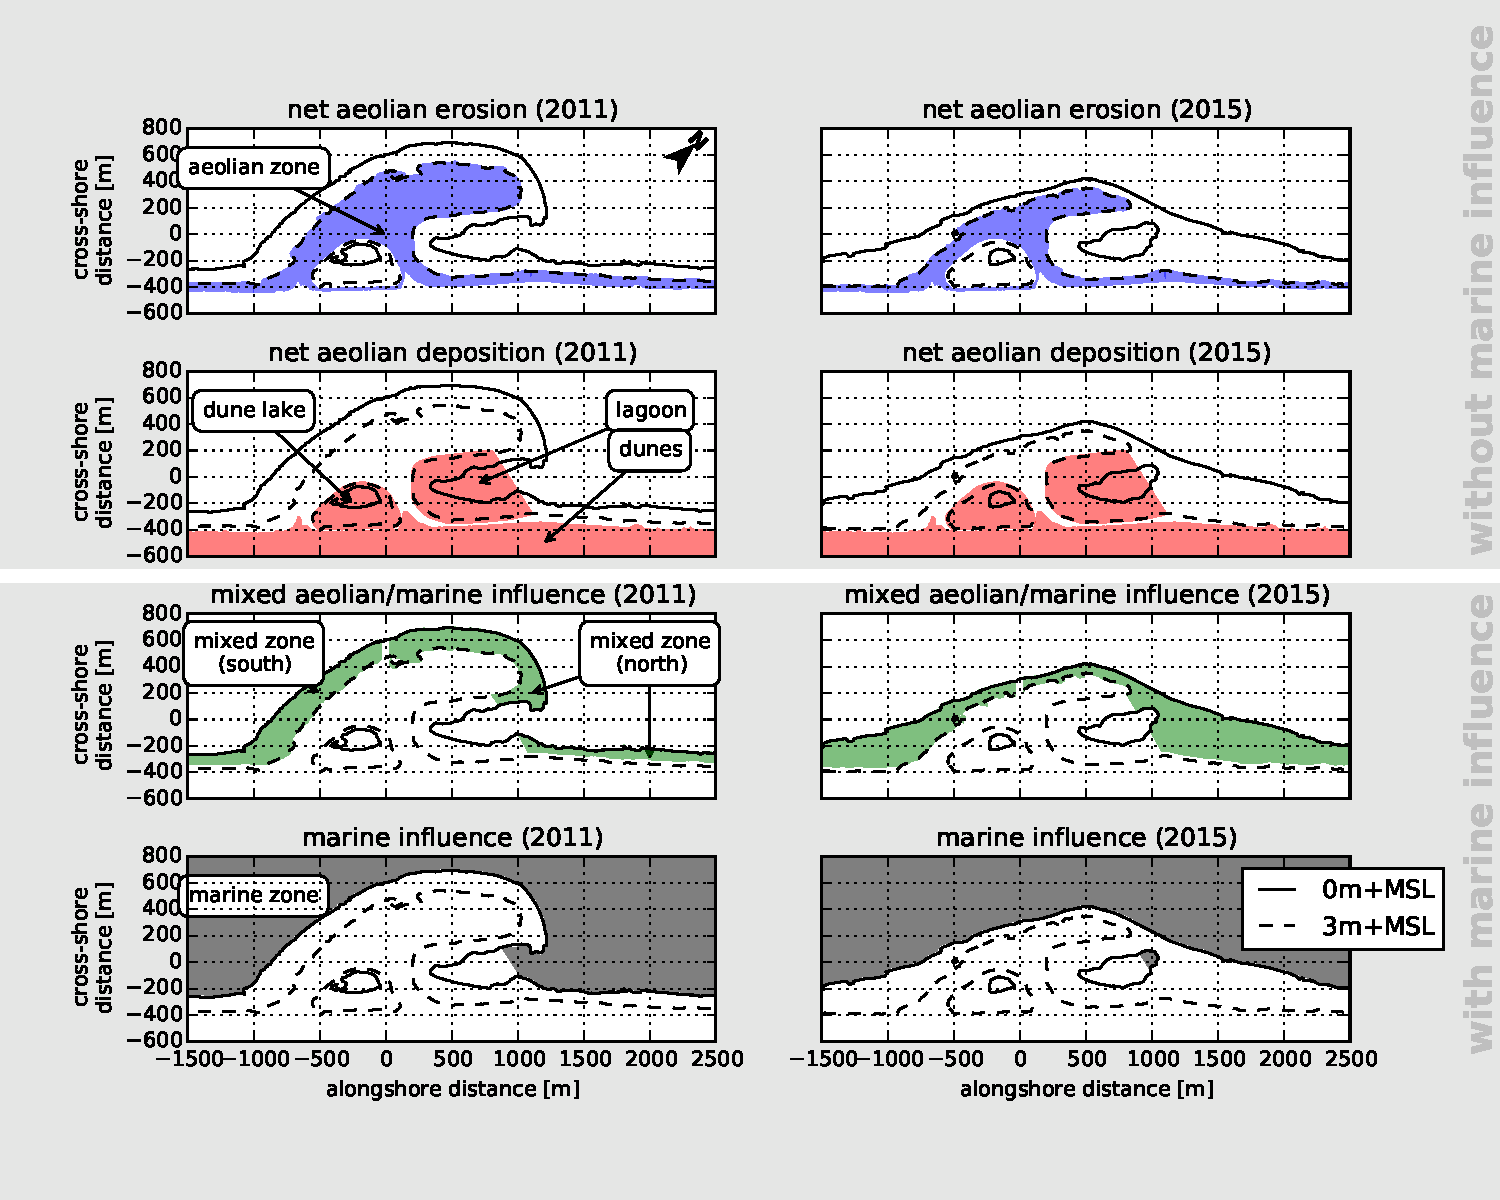
\includegraphics[width=\columnwidth]{../Figures/decomposition}
  \caption{Zonation of the Sand Motor domain into zones with net
    aeolian erosion and no marine influence, net aeolian deposition
    and no marine influence, mixed aeolian/marine influence and marine
    influence. Left panels: 2011. Right panels: 2015.}
  \label{fig:decomposition}
\end{figure}

The Sand Motor domain is divided into seven zones for the aeolian
sediment budget analysis (Table \ref{tab:decomposition} and Figure
\ref{fig:decomposition}). The zonation aims to separate areas with
marine influences from areas without marine influences, and separate
areas with net aeolian erosion from areas with net aeolian deposition.

\begin{table}[h!]
  \centering
  \caption{Zonation of the Sand Motor domain into seven zones with and
    without marine influence. See also Figure \ref{fig:decomposition}.}
  \label{tab:decomposition}
  \begin{tabularx}{\textwidth}{XX}
    \emph{without} marine influence  & \emph{with} marine influence \\
    \hline
    aeolian zone                     & mixed zone (north)           \\
    dunes                            & mixed zone (south)           \\
    dune lake                        & marine zone                  \\
    lagoon                           &                              \\
  \end{tabularx}
\end{table}

The zonation is based on the 0 m+MSL, 3 m+MSL and 5 m+MSL contour
lines that roughly correspond to mean sea level, the edge of the berm
or maximum runup level (Figure \ref{fig:windwaves}c) and the dune foot
respectively. The contours are determined such that the spatial
variance in the bed level change of the zones is minimized. The
minimization ensures that the optimal division between erosion and
deposition areas is found. Moreover, the 3 m+MSL and 5 m+MSL contour
lines have been relatively static since construction of the Sand
Motor.

To ensure a constant shape and size of the zones during the analysis,
the convex hull of all 3 m+MSL contour lines is used as zone boundary
for the lake and lagoon. Also for the dunes minimal variations over
time in zone shape and size are removed by using the most seaward
position of all contour lines. Consequently, only the aeolian zone and
mixed zones change in shape and size over time. The volumetric change
between two consecutive measurements is determined for these zones
within the smaller contour:

\begin{equation}
  \Delta V^n = \hat{A}_{\mathrm{c}} \cdot \left( \overline{z_{\mathrm{b}}}^n - \overline{z_{\mathrm{b}}}^{n-1} \right)
  \quad \mathrm{where} ~ \hat{A}_{\mathrm{c}} = \min \left( A_{\mathrm{c}}^n ~;~ A_{\mathrm{c}}^{n-1} \right)
\end{equation}

\noindent with $\Delta V^n$ the volume change, $A_{\mathrm{c}}^n$ the
surface area of the zone and $\overline{z_{\mathrm{b}}}^n$ the average
bed level in the zone, all in time interval $n$. The (cumulative) sum
over all time intervals of the volume changes in each zone is used in
the analysis. By using the smaller of two contours in a comparison, a
part of the larger contour is neglected:

\begin{equation}
  A^n_{\mathrm{c,neglected}} = \max \left( A_{\mathrm{c}}^n ~;~ A_{\mathrm{c}}^{n-1} \right) - \hat{A}_{\mathrm{c}}
\end{equation}

\noindent The neglected area of the zone with the largest change in
size, the aeolian zone, is on average 2\% and never larger than 8\%.

\subsection{Spatial variations in porosity}

The change in sediment volume is susceptible to changes in
porosity. In order to relate the changes in sediment volume to the
transport of sediment mass, variations in porosity need to be
accounted for. Porosity values in the Sand Motor domain are obtained
from core samples and used to account for the spatial variations in
porosity. The core samples have a diameter of 8 cm and depth of 10 cm
from the bed surface in an attempt to capture the porosity in the
aeolian active layer of the bed. Each sample is dried and submerged in
water to determine the porosity. For comparison, all presented
sediment volumes in this paper are converted to a hypothetical
porosity of 40\% according to:

\begin{equation}
  V_{\mathrm{40\%}} = V \cdot \frac{1 - p}{1 - 40\%}
\end{equation}

\noindent where $V$ [$\mathrm{m^3}$] is the measured sediment volume
and $p$ [-] the porosity.

\section{Results}

\begin{figure}
  \centering
  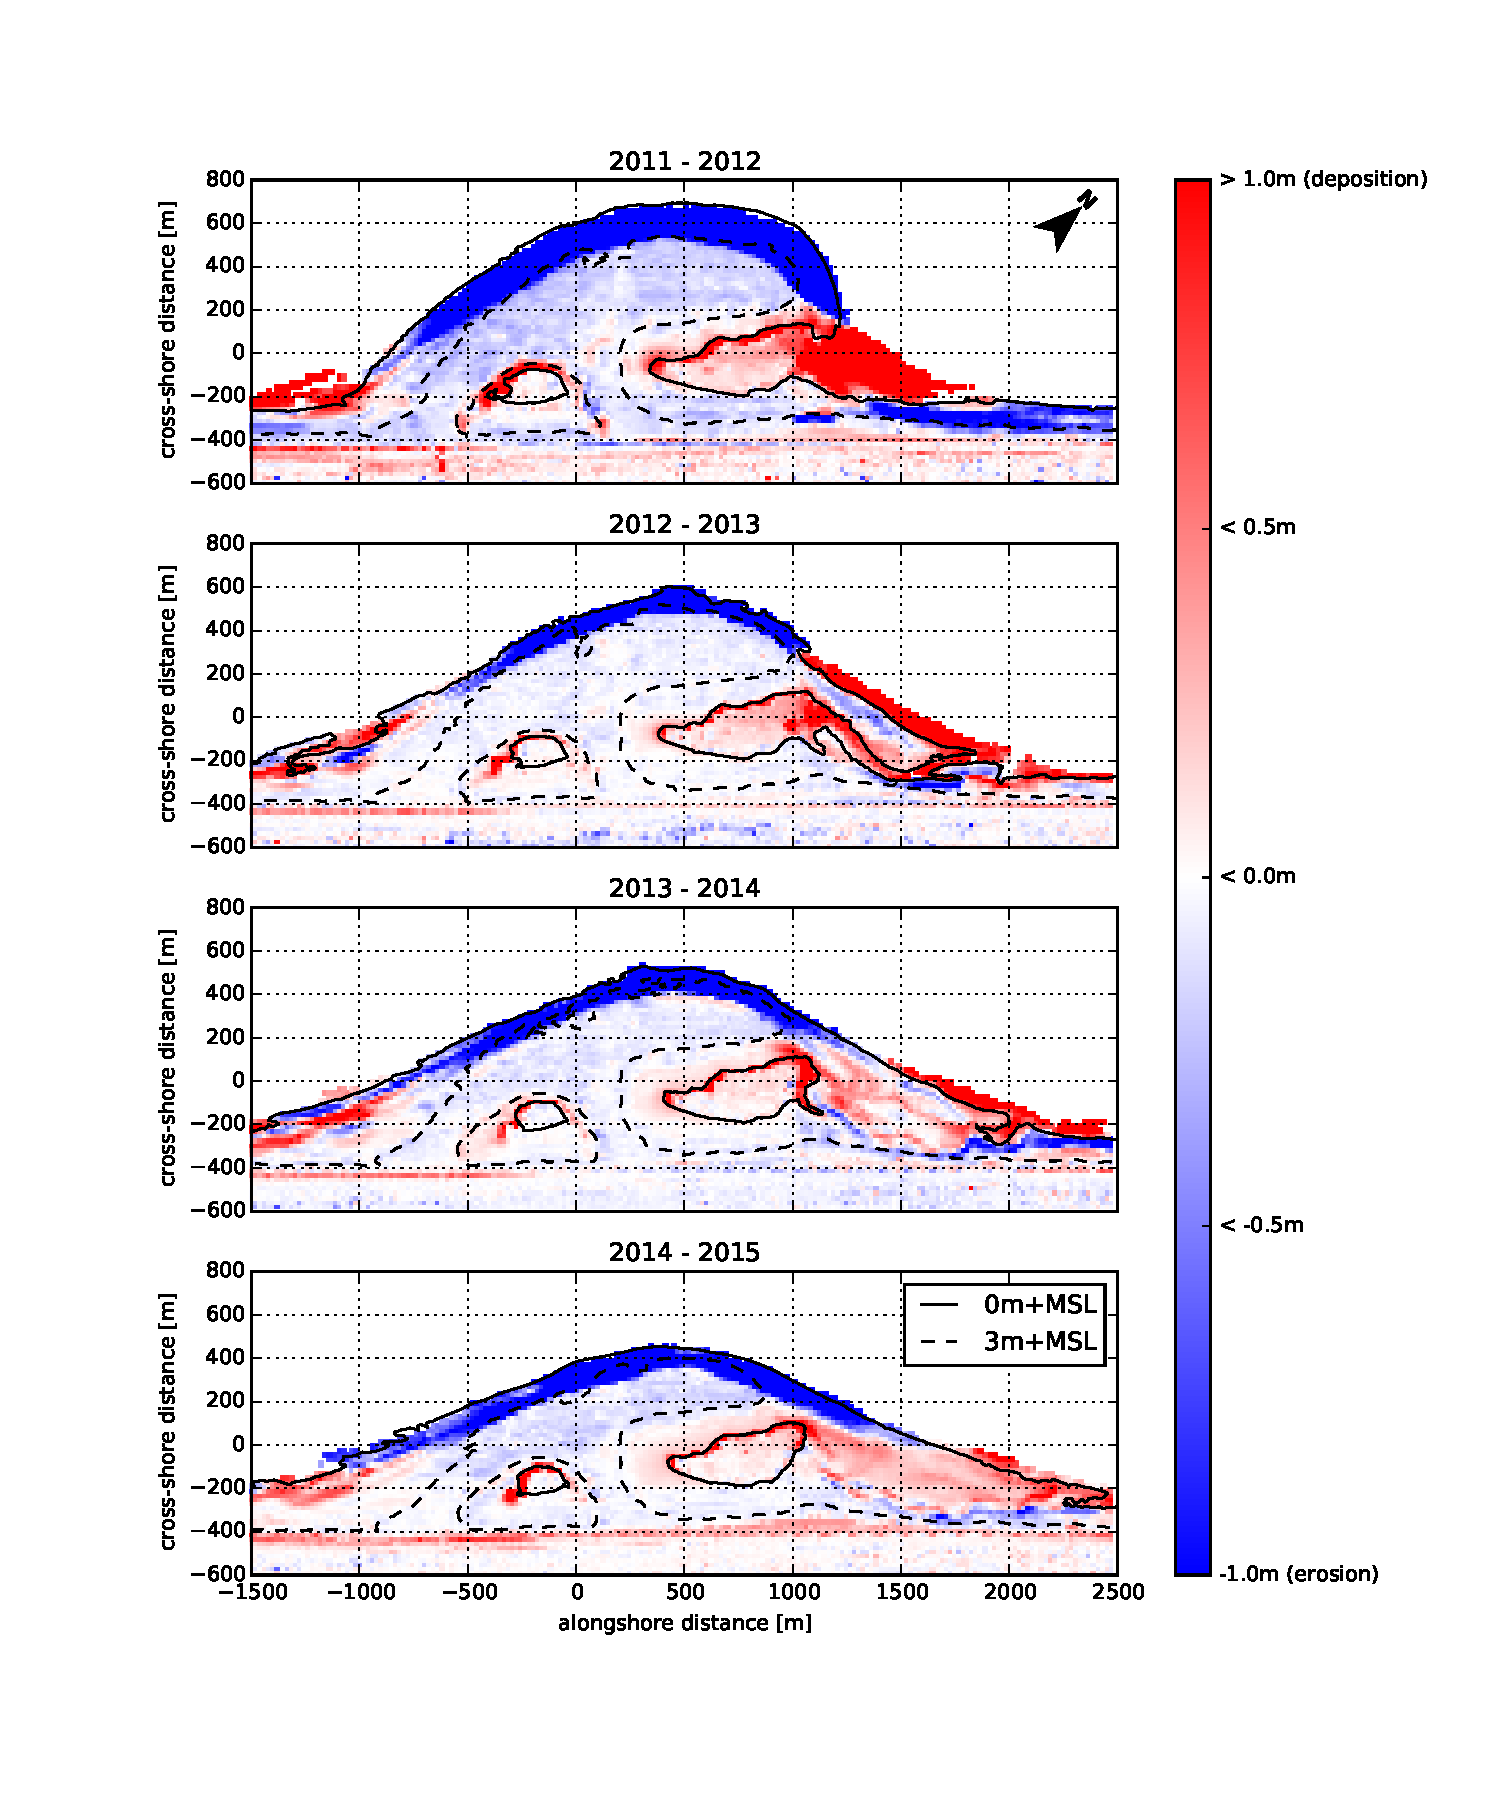
\includegraphics[width=\columnwidth]{../Figures/sedero}
  \caption{Yearly sedimentation and erosion above 0 m+MSL in the Sand
    Motor domain. Comparisons are made between the September surveys
    of each year.}
  \label{fig:sedero}
\end{figure}

The overall sediment budget of the Sand Motor domain is determined
given morphological change in the net aeolian erosion and net aeolian
deposition zones for the period between September 1, 2011 and
September 1, 2015 (Figure \ref{fig:sedero}).

\subsection{Morphological change and porosity}

The net morphological change within the 3 m+MSL contour can be
accredited entirely to aeolian sediment transport as this area is not
significantly affected by marine processes since the construction of
the Sand Motor. Also the net contribution of alongshore sediment
fluxes are assumed to be relatively small given that the beach width
($<$ 100 m) is small compared to the alongshore span of the
measurement domain (4 km). Within the 3 m+MSL contour sediment is
deposited in the dunes and eroded from the aeolian zone.

The morphological change in the dune lake and the closed end of the
lagoon is assumed to be driven predominantly by wind. Hydrodynamic
forcing and consequently marine deposits in these zones diminished
quickly over time, while significant amounts of fine aeolian deposits
are found along the southwestern to northwestern shores. \mrq[ls]{1.3}

The aeolian contribution to the morphological change in the mixed
zones cannot be determined directly due to the presence of both marine
and aeolian forces. However, by balancing the changes in sediment
volume in the net aeolian deposition zones with the changes in
sediment volume in the net aeolian erosion zones the aeolian sediment
supply from the mixed zones is estimated. \mrq[ls]{1.1}

18 porosity measurements from six zones (Table \ref{tab:porosity}) are
used to convert all measured sediment volumes to a hypothetical
porosity of 40\%.

\begin{table}
  \centering
  \caption{Measured porosity values in the Sand Motor domain. Each
    area is sampled at three different locations. The results per area are
    presented in ascending order. The last column presents the average
    porosity for each area that is used to convert the sediment volumes
    presented in this paper to a hypothetical porosity of 40\%.}
  \label{tab:porosity}
  \begin{tabular}{lrrrr}
    Area                     & \multicolumn{4}{c}{Porosity}      \\
                             & min.   &        & max.   & avg.   \\
    \hline 
    Aeolian zone             & 39.0\% & 39.4\% & 40.2\% & 39.5\% \\
    Mixed zone (north)       & 38.4\% & 39.8\% & 40.8\% & 39.7\% \\
    Mixed zone (south)       & 37.1\% & 38.4\% & 38.4\% & 38.0\% \\
    Dunes                    & 36.1\% & 36.3\% & 37.1\% & 36.5\% \\
    Dune lake                & 34.7\% & 34.9\% & 36.3\% & 35.3\% \\
    Lagoon                   & 46.3\% & 47.3\% & 49.0\% & 47.6\% \\
  \end{tabular}
\end{table}

\subsection{Aeolian sediment budgets}
\label{sec:budgets}

\begin{figure}
  \centering
  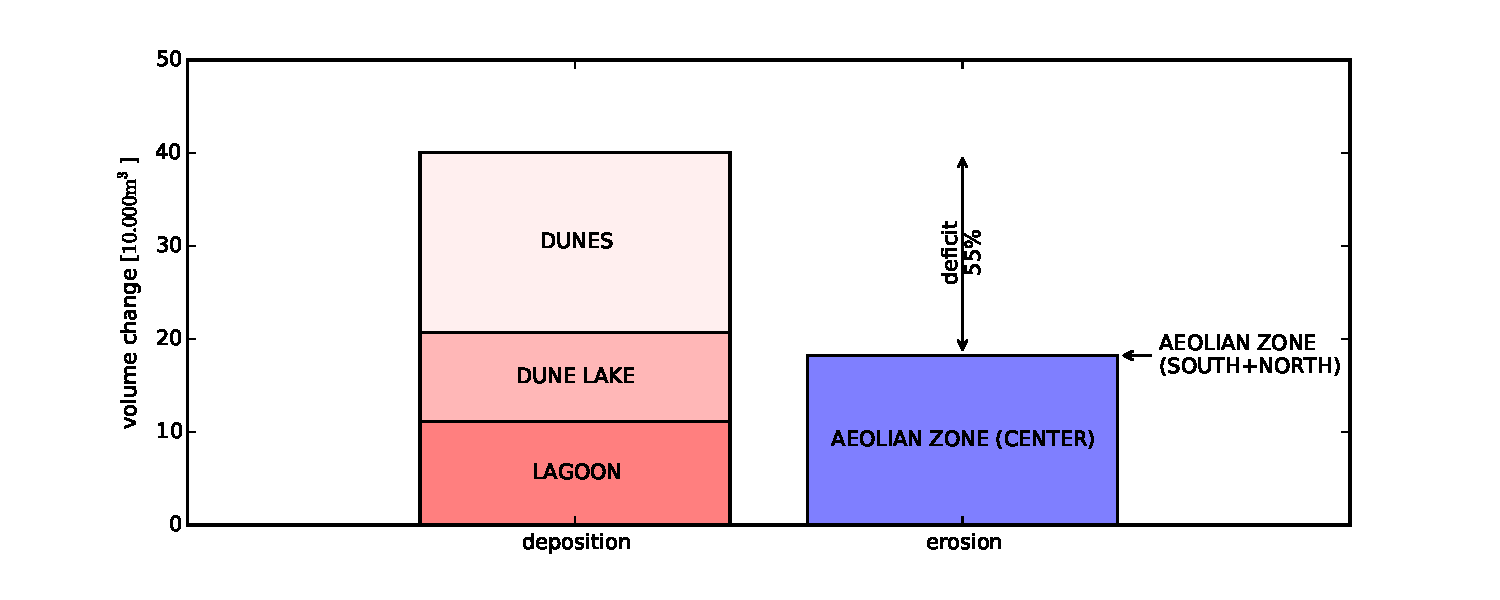
\includegraphics[width=\columnwidth]{../Figures/volumes_bars}
  \caption{Aeolian sediment budgets in the Sand Motor domain in the
    period between September 1, 2011 and September 1, 2015.}
  \label{fig:volumes_bars}
\end{figure}

The aeolian zone consistently provides less sediment than is deposited
in the dunes, dune lake and lagoon (Figure
\ref{fig:volumes_bars}). Over the four years since construction of the
Sand Motor the volume deficit accumulates to $\mathrm{21 \cdot 10^4}$
$\mathrm{m^3}$, which is 52\% of the total sediment accumulation of
$\mathrm{40 \cdot 10^4}$ $\mathrm{m^3}$. \mrq[ls]{1.2} The total wind
transport capacity (or cumulative theoretical sediment transport
volume) in this period is roughly estimated as
$\mathrm{110 \cdot 10^4}$ $\mathrm{m^3}$ (Appendix
\ref{apx:theoretical_transport}). As the actual sediment transport
rates appear to be only about 35\% of the wind transport capacity, the
Sand Motor can be classified as an availability-limited system.

Late January 2012, the surveys show a net volume deficit of zero,
while subsequent surveys show a more or less linear growth of the
volume deficit (Figure \ref{fig:netvolumechange}). Fitting a linear
trend reveals an average growth rate of $\mathrm{5.2 \cdot 10^4}$
$\mathrm{m^3/yr}$, which is 67\% of the total sediment accumulation
rate of $\mathrm{7.7 \cdot 10^4}$ $\mathrm{m^3/yr}$ ($\mathrm{R^2}$ =
0.96). The increase in growth rate of the volume deficit is likely
caused by a significant decrease of the sediment contribution from the
aeolian zone. The erosion from the aeolian zone in the first half year
after construction of the Sand Motor exceeds the total erosion in the
four years thereafter, while sediment continued to be accumulated in
the dunes, dune lake and lagoon. The surface area of the aeolian zone
decreased continuously (Figure \ref{fig:areas}).

\begin{figure}
 \centering
  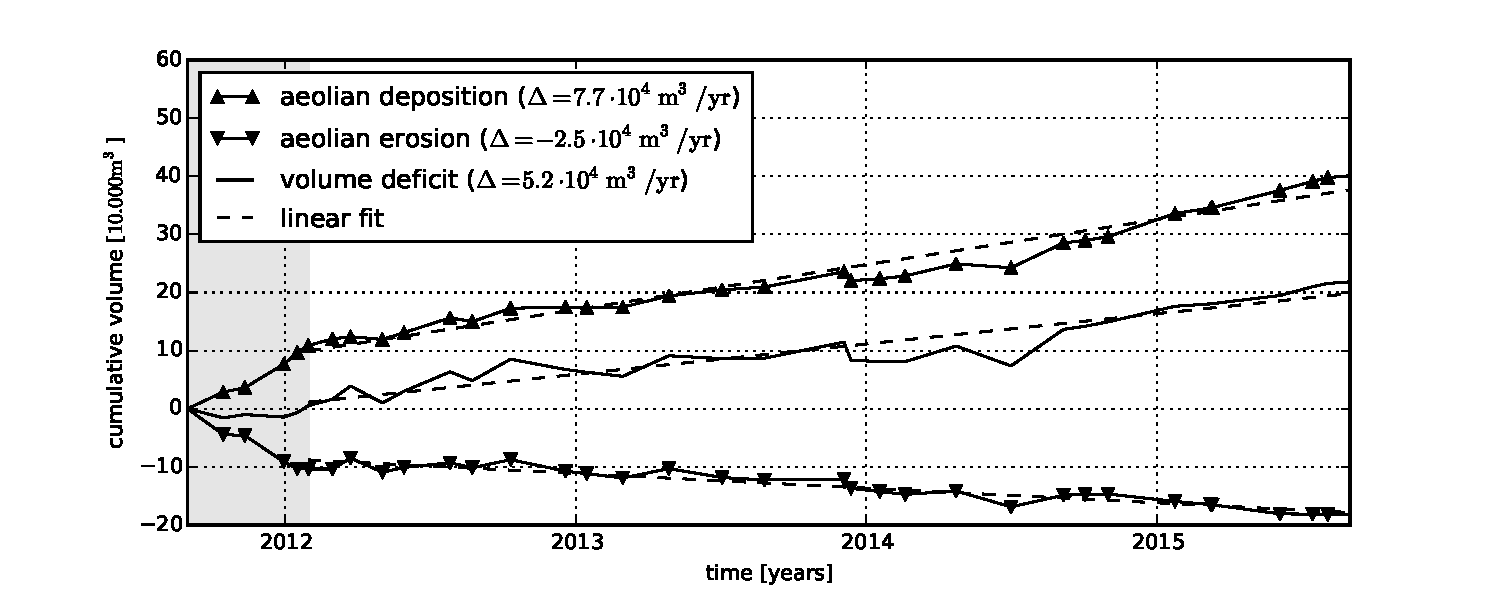
\includegraphics[width=\columnwidth]{../Figures/netvolumechange}
  \caption{Cumulative change in sediment volume of all net aeolian
    erosion and net aeolian deposition zones and the volume
    deficit. For the linear fit the period prior to February 2012 is
    discarded (shaded).}
  \label{fig:netvolumechange}
\end{figure}

\begin{figure}
  \centering
  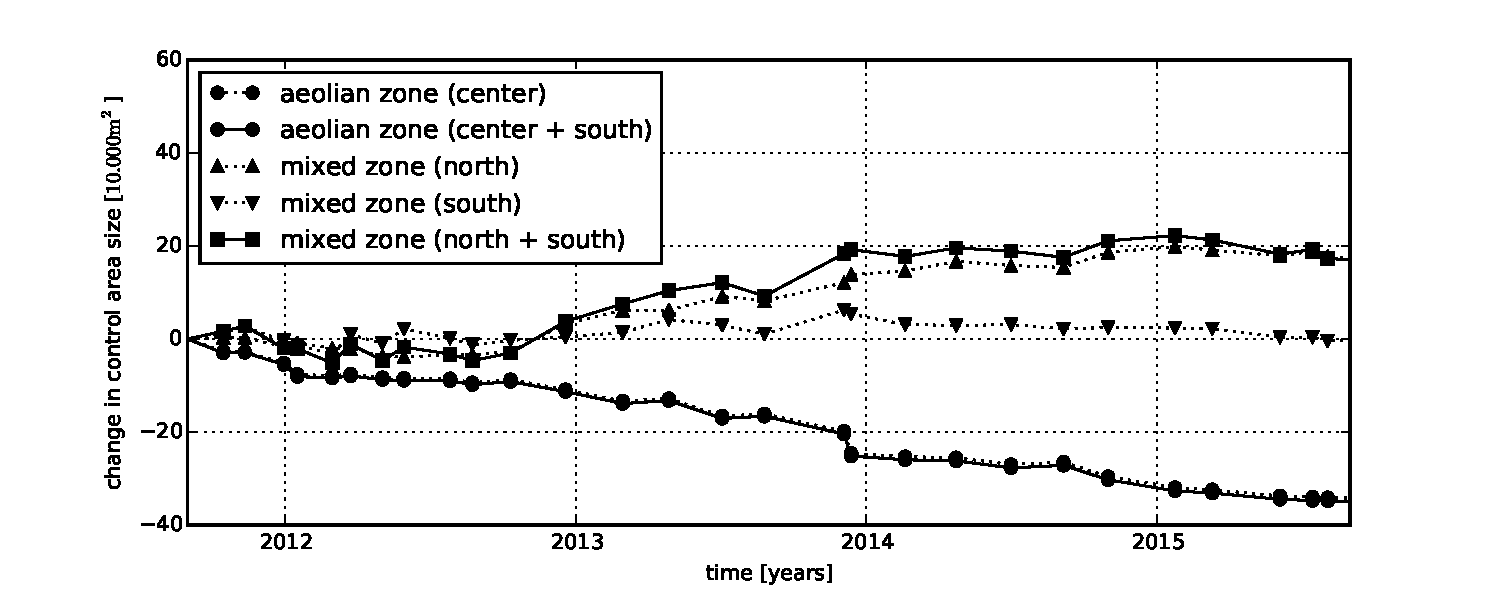
\includegraphics[width=\columnwidth]{../Figures/areas}
  \caption{Change in size of aeolian zone and mixed zones since
    construction of the Sand Motor in 2011.}
  \label{fig:areas}
\end{figure}

The diminishing of the aeolian sediment supply from the aeolian zone
is also reflected in the average bed level within the 3 m+MSL contour
of September 22, 2015 (Figure \ref{fig:heights}). The bed level within
this contour has been almost constant since the volume deficit started
to grow steadily from late January 2012. Only a few periods of
significant erosion can be distinguished that can be related to storm
events. Most notably, the event of December 5, 2013 with wind speeds
up to 34 m/s. That day $\mathrm{1.5 \cdot 10^4}$ $\mathrm{m^3}$ of
sediment was eroded from within the 3 m+MSL contour of September 22,
2015, which is 52\% of the total erosion that year. Although this
event is among the few events during which the runup levels exceeded
the 3 m+MSL level (Figure \ref{fig:windwaves}), the erosion can still
be accredited to wind as the 3 m+MSL contour of September 22, 2015 was
located about 100 m landward of the 3 m+MSL contour at the time of the
storm event. Therefore the bed level in the more recent contour was
not affected by the surge, which is confirmed by observations from a
local permanent camera station.% (Figure \ref{fig:argus}).

In general, the use of the 3 m+MSL contour as divide between the areas
with and without marine influence appears to be valid for almost the
entire four years after construction of the Sand Motor. Only four
events have been registered in which runup levels exceeded the 3 m+MSL
level (Figure \ref{fig:windwaves}). Observations from a local
permanent camera station indicate that only during the event of
December 5, 2013 the surface of the aeolian zone was significantly
affected by tides and waves. Pre- and post-storm topographic surveys
that are available for this event indicate that the marine erosion
from the flooded areas above the 3 m+MSL level was less than
$\mathrm{1 \cdot 10^4}$ $\mathrm{m^3}$.

%Additional visual observations of the Sand Motor surface indicate that
%a coarse beach armor layer developed over time that consists of coarse
%sand, shell fragments and shells.% (Figure \ref{fig:armoring}).

\begin{figure}
  \centering
  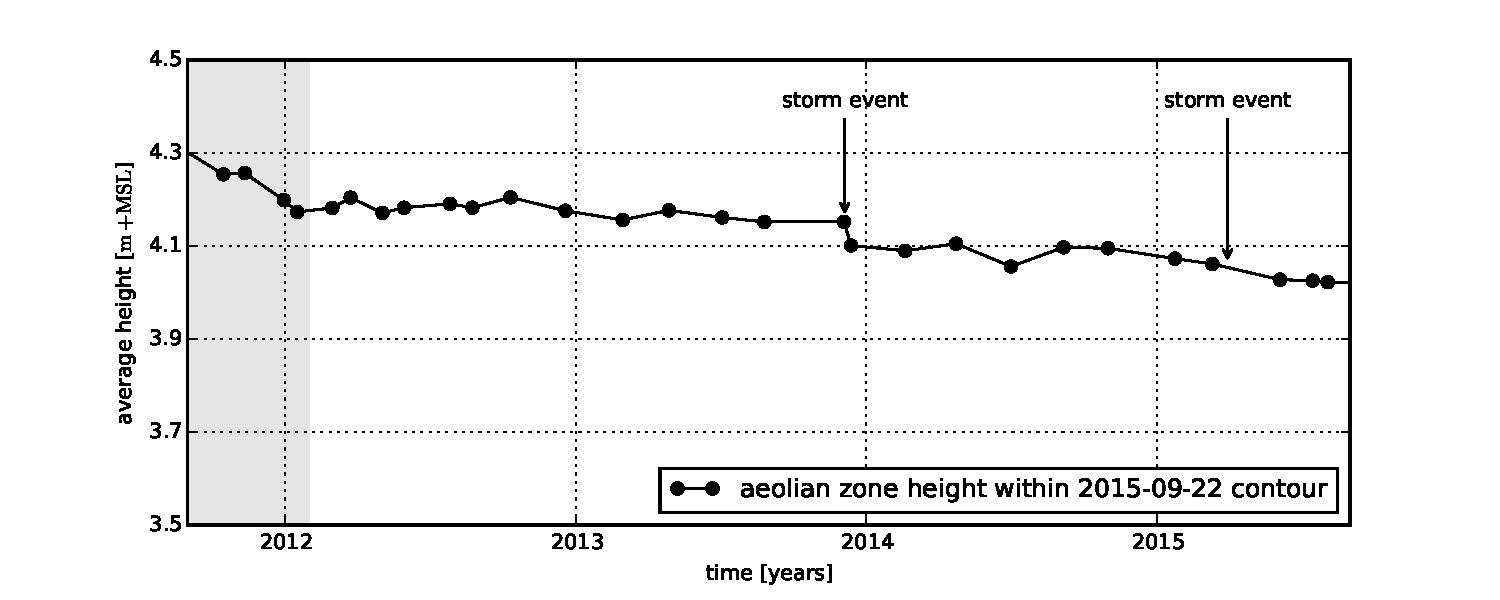
\includegraphics[width=\columnwidth]{../Figures/heights}
  \caption{Average height of the aeolian zone in the most recent
    contour.}
  \label{fig:heights}
\end{figure}

%\begin{figure}
%  \centering
%  \includegraphics[width=\columnwidth]{../Figures/argus}
%  \caption{Image from the local permanent camera station at the Sand
%    Motor from December 6, 2013 with the 3 m+MSL contour of September
%    22, 2015. The image is georectified using the \textsc{Flamingo}
%    toolbox \citep{Hoonhout2015a}.}
%  \label{fig:argus}
%\end{figure}

%\begin{figure}
%  \centering
%  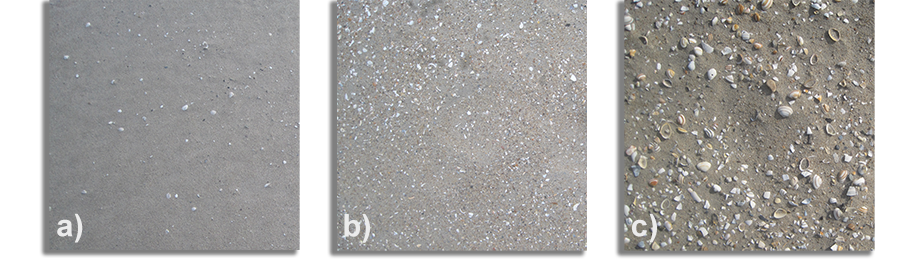
\includegraphics[width=\columnwidth]{../Figures/armoring_small}
%  \caption{Visual impression of armor layer at three locations in the
%    Sand Motor region: a) intertidal beach, no armoring b) lower dry
%    beach, minor armoring with shell fragments c) upper dry beach,
%    severe armoring with many shells and coarse sand. Covered surface
%    is approximately 40 cm x 40 cm in all cases.}
%  \label{fig:armoring}
%\end{figure}

\subsection{Alongshore variation}

The sediment deposits in the dunes show an alongshore
variation\mrq[ls]{2.4}. A depression in dune growth is observed in the
lee of the dune lake and lagoon (Figure
\ref{fig:adjacentcoasts}). South of the dune lake and in between the
dune lake and lagoon a passage for aeolian sediment transport is
present, which seems to result in a locally elevated dune growth. The
average dune growth of 14 $\mathrm{m^3/m/yr}$ in the Sand Motor domain
is low compared to the dune growth rate along the adjacent southern
(15 $\mathrm{m^3/m/yr}$) and northern (19 $\mathrm{m^3/m/yr}$) beach
stretches.  However, aeolian deposits in the dune lake and lagoon are
of the same order of magnitude resulting in a total average sediment
deposition of 27 $\mathrm{m^3/m/yr}$ in the Sand Motor domain, which
is on average 56\% higher than along the adjacent coasts.

\begin{figure}
 \centering
  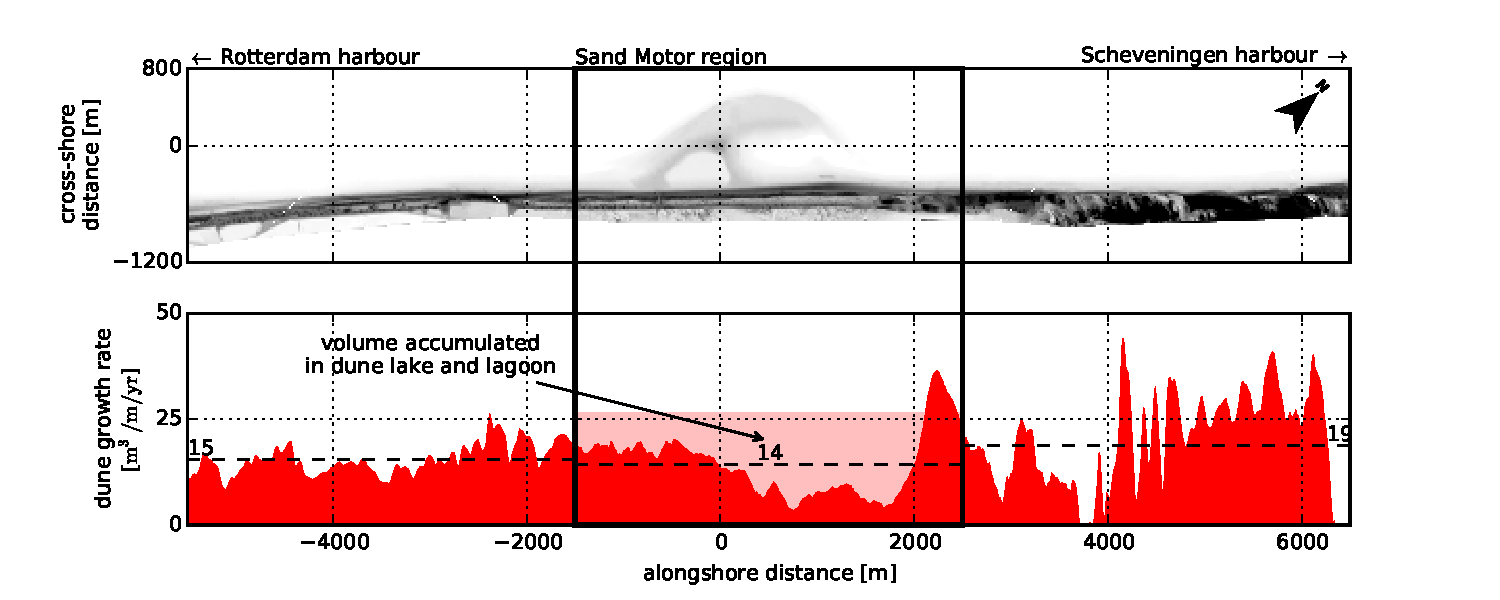
\includegraphics[width=\columnwidth]{../Figures/adjacentcoasts}
  \caption{Comparison sediment accumulation rates in dunes
    (\textgreater 3 m+MSL) for Sand Motor domain and adjacent
    coasts. Airborne lidar measurements from January 2012 until
    January 2015 are used. Horizontal dashed lines indicate local
    averages. The box indicates the Sand Motor domain depicted in
    previous figures.}
  \label{fig:adjacentcoasts}
\end{figure}

\section{Discussion}

% southern intertidal beach is main supplier of aeolian sediment
The volume deficit between the net aeolian erosion and net aeolian
deposition zones can be accredited to the mixed zones that are
affected by both marine and aeolian processes. The mixed zones in the
Sand Motor domain are consequently estimated to provide 67\% of the
aeolian sediment in the Sand Motor domain. \mrq[ls]{1.4} The aeolian
sediment supply from the mixed zones is therefore significant, but
still small compared to the 98\% reported by \citet{Jackson2010}. The
importance of the mixed zone cannot be explained by the size of the
surface area as the mixed zones are initially smaller than the other
main sediment source: the aeolian zone (Figure \ref{fig:areas}). Only
from 2013 onward the surface area of the mixed zones exceed the area
of the aeolian zone. However, the increase in surface area of the
mixed zones is concentrated in the north where a low-lying spit
develops (Figure \ref{fig:sedero}). Given the dominant south to
southwesterly wind direction and their position with respect to the
lagoon that separates the spit from the dunes, it is unlikely that
these intertidal beaches, provide a significant amount of sediment to
dunes, dune lake and lagoon. Therefore, despite the periodic flooding
and a size that is 40\% -- 60\% smaller than the aeolian zone, the
mixed zone (south) appears to provide the majority of the aeolian
sediment in the Sand Motor domain.

\subsection{Sources of inaccuracies}

By accrediting the volume deficit to the mixed zones it is assumed
that no sediment is exchanged over the boundaries of the Sand Motor
domain and the sediment volume balance is thus closed. This assumption
is not strictly valid, but the external sediment exchange with the
Sand Motor domain is limited compared to the total sediment
accumulation of $\mathrm{40 \cdot 10^4}$ $\mathrm{m^3}$.

\begin{figure}
  \centering
  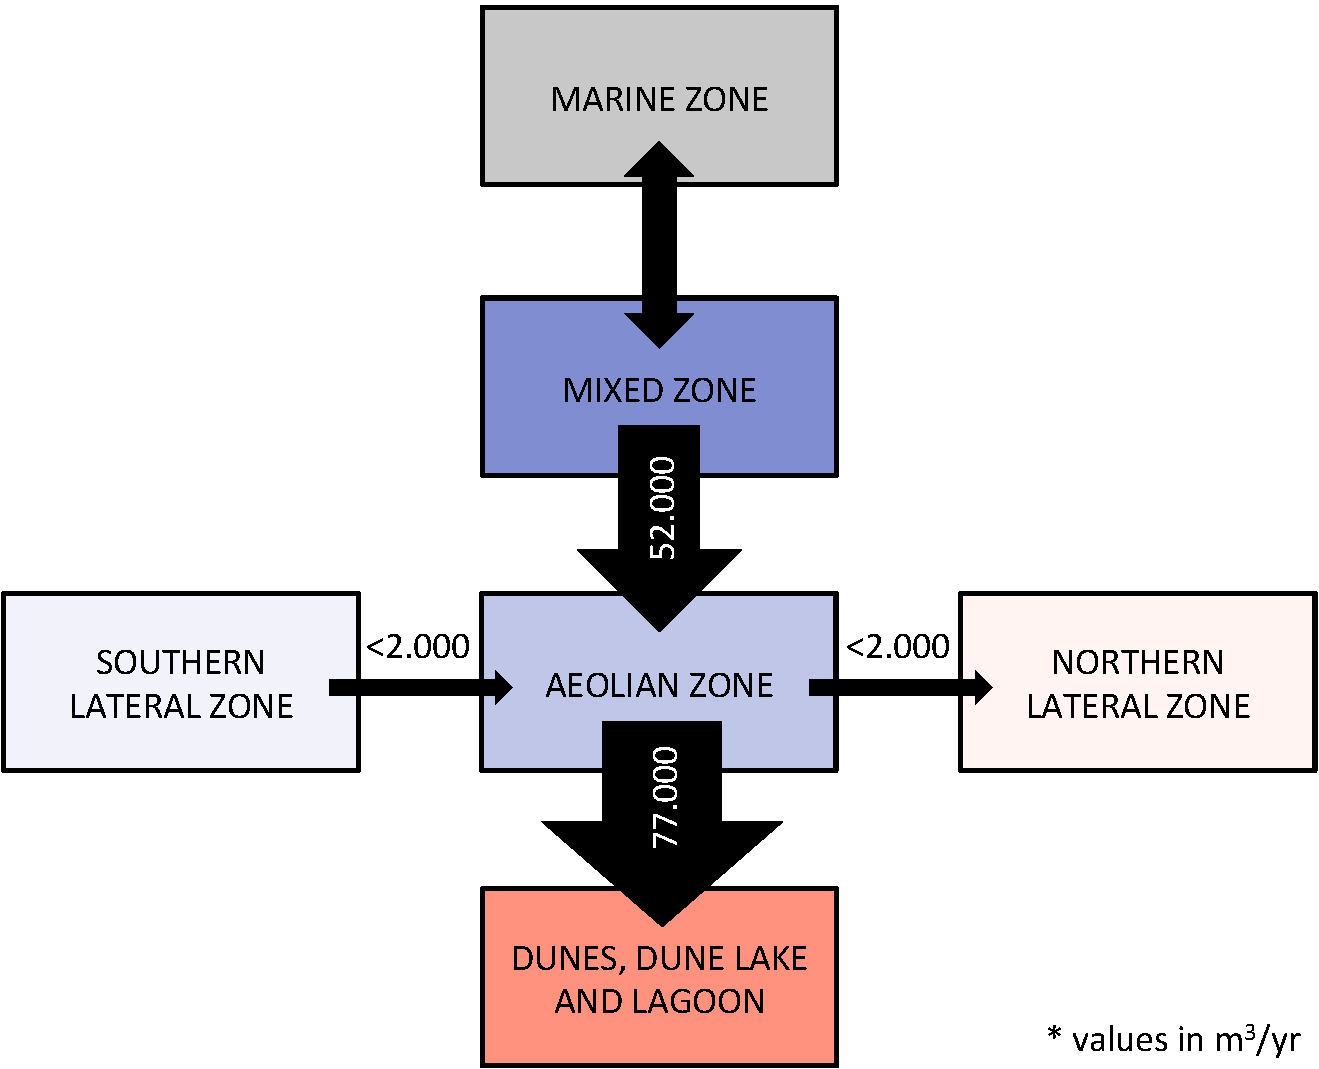
\includegraphics[width=\columnwidth]{../Figures/budgets}
  \caption{Aeolian sediment budget analysis of the Sand Motor}
  \label{fig:budgets}
\end{figure}

The predominantly southwesterly wind direction might blow sediment
over the lateral borders that is not taken into account. However, the
net alongshore sediment supply to the Sand Motor domain is estimated
to be two orders smaller than the net onshore sediment supply, or less
than 1\% of the total sediment accumulation (Figure
\ref{fig:budgets}), because:

\begin{enumerate}
\item The onshore and alongshore sediment flux \emph{per meter width}
  are estimated to be of the same order of magnitude (Appendix
  \ref{apx:theoretical_transport}), but the lateral beach
  cross-section ($< 100$ m) through which the alongshore flux enters
  the Sand Motor domain at the southern border is an order of
  magnitude smaller than the alongshore span of the Sand Motor domain
  (4 km) through which the onshore flux enters the domain. Therefore,
  the absolute alongshore contribution to the total sediment volume
  balance is likely an order of magnitude smaller than the onshore
  contribution.
\item The contribution of the net alongshore sediment flux that enters
  the Sand Motor domain at the southern border is at least partially
  compensated by a net alongshore sediment flux of the same order of
  magnitude that leaves the domain at the northern border. Therefore,
  the contribution to the total sediment volume balance of the
  southern and northern alongshore sediment fluxes combined
  (alongshore sediment transport gradient) is likely two orders of
  magnitude smaller than the contribution of the onshore sediment
  flux.
\end{enumerate}

\noindent In reality the contribution of the alongshore sediment
fluxes is likely to be even smaller as the sediment fluxes can locally
be more onshore directed due to local wind steering. In addition, the
estimates of the order of magnitude of the sediment fluxes are likely
to be overestimated as possible limitations in sediment availability
are ignored.

%Finally, the combined alongshore sediment fluxes are expected to be a
%net sediment sink (of negligible magnitude) as the net alongshore
%fluxes, dune profile and dune growth along the Dutch coast were
%remarkably constant and uniform prior to construction of the Sand
%Motor \citep{Arens2010, deVries2012b}. After construction of the Sand
%Motor only the source area of the northern alongshore sediment flux
%grew tremendously, while the source area of the southern alongshore
%sediment flux did not change. Consequently, only the northern net
%alongshore sediment flux might have changed and likely increased
%increased, resulting in a net sediment sink as it leaves the Sand
%Motor domain.

The influence of marine deposits in the lagoon is estimated to be less
than 4\% of the total sediment accumulation. 85\% of the deposited
sediment in the lagoon has the form of a southwesterly infill
protruding above water and consisting of loosely packed, fine sediment
and is therefore likely from aeolian origin (Figure \ref{fig:sedero}
and Table \ref{tab:porosity}). 15\% of the deposited sediment in the
lagoon, or 4\% of the total sediment accumulation, is spread over a
wider area and is possibly from marine origin.

The influence of marine erosion of the aeolian zone during the limited
number of storm surges is estimated to be less than
$\mathrm{1 \cdot 10^4}$ $\mathrm{m^3}$ (Section \ref{sec:budgets}), or
2.5\% of the total sediment accumulation. Similarly, the influence of
the changing size of the aeolian zone is estimated to be 2\% of the
total erosion in this area (Section \ref{sec:zonation}), or less than
1\% of the total sediment accumulation.

In summary, the error that is introduced by assuming a closed sediment
volume balance is estimated to be less than 9\% of the total sediment
accumulation. The volume deficit of 67\% of the total sediment
accumulation that is accredited to aeolian erosion from the mixed
zones therefore needs to be nuanced and is estimated to be more than
58\%.

% supply from dry beach dies out because of beach armoring
\subsection{Beach armoring}

The relative importance of the mixed zones for aeolian sediment supply
can likely be explained by a visually observed beach armor layer that
developed in the aeolian zone since construction of the Sand Motor. A
beach armor layer can reduce the availability of aeolian sediment
significantly \citep{McKennaNeuman2012}. Because the Sand Motor was
constructed several meters above common storm surge level, the aeolian
zone has never been influenced by waves or tides. Consequently, no
process is present that regularly resets the armor layer, except for
the occasional high-energy wind event. Moreover, salt crusts that form
due to salt spray have a similar effect on the sediment availability
as an armor layer. Small concentrations of salt
($\mathrm{\leq 7 ~ mg/g}$) can already reduce the sediment
availability by a factor two \citep{Nickling1981}. \mrq[ls]{1.5}

In contrast, no beach armor layer or salt crusts develop in the mixed
zones as periodic flooding and related wave-reworking regularly
deposit marine sediments, mix the top layer of the bed, and wash
shells and shell fragments away. In addition, onshore bar migration
and welding periodically provide additional unarmored sediment that
can be entrained by the wind during low water \citep{Houser2009,
  Anthony2013}. However, aeolian sediment availability in the mixed
zones is also limited due to the relatively high soil moisture
contents in these areas. Also soil moisture content is known to
increase the shear velocity threshold \citep{Wiggs2004, Edwards2009,
  Namikas2010} and limit the local aeolian sediment availability.
Given that the mixed zones appear to be a more important supplier of
aeolian sediment than the aeolian zone, limitations in sediment
availability due to beach armoring seems to outweigh limitations due
to high moisture contents.

% beach armoring can be broken only by extreme events
During a storm event even shell fragments and shells can be
mobilized. Consequently, the beach armor layer itself might be
transported and its reducing effect on the sediment availability is
(partially) neutralized. Storm events are regularly accompanied with
surges that prevent wind erosion of the mixed zones. Entrainment of
sediment therefore starts at a relatively high point along the fetch
and much of the sediment transport capacity can be used for erosion of
the aeolian zone, which contributes to the removal of the beach armor
layer. If the surge is high enough it can also remove the beach armor
layer by wave action or bury it by deposition of marine sediments. The
removal or burial of the beach armor layer can elevate sediment
availability from the aeolian zone also after the the storm
passed. Only after development of a new beach armor layer the sediment
availability and transport rates approach the pre-storm
situation.
% Similarly, rain showers can flush the salts (partially) from the
% bed, increasing the sediment availability as well.

\subsection{Mega nourishments as coastal protection}

The Sand Motor mega nourishment shows a morphological development that
is significantly different from natural beaches or the original
Delfland coast. Aeolian sediment supply at the Sand Motor shows larger
spatial variations compared to natural beaches, while dune growth
rates lag behind compared to the adjacent coastal stretches. It can be
questioned if such exotic behavior is desired for a coastal protection
that aims to stimulate natural processes, or that, for example, it
would be beneficial not to construct future mega nourishments above
local storm surge level and prevent compartmentalization of the beach.

In this context, it is interesting to consider what would happen if
the Sand Motor was constructed up to local storm surge level (3
m+MSL). The vast aeolian zone would not exist as the entire Sand Motor
would be flooded at least once a year. Compartmentalization would be
minimized and aeolian sediment availability be maximized as the
formation of deflation lag deposits is counteracted by
wave-reworking. The dune lake and lagoon would be filled in up to
three times faster due to transport-limited aeolian sediment
supply. Soon, all aeolian sediment transport pathways would end in the
dunes, resulting in an up to six times larger dune growth than
currently observed. Marine sediment transport would enhance these
relatively rapid changes as more sediment is redistributed within the
Sand Motor domain to the lagoon, dune lake and offshore by overwash.

A lower construction height of the Sand Motor would therefore result
in a more rapid and more localized redistribution of sediment. Both
rapid and localized redistribution are at odds with the purpose of the
Sand Motor to nourish the entire Holland coast over a period of two
decades. The static behavior of the supratidal areas of Sand Motor
might therefore prove to be a crucial design criterion of a mega
nourishment.

% variation in dune growth rate, beach surface area
%\subsection{Beach width vs. coastline length}
%
%The intertidal beach area or, assuming an alongshore uniform
%intertidal beach slope, the coastline length seems to be a better
%indicator for coastal aeolian sediment transport than fetch or dry
%beach area. The total aeolian sediment deposits in the the dunes, dune
%lake and lagoon, exceed the aeolian deposits along the adjacent coasts
%with 56\% on average. Although significant, the increase in aeolian
%sediment deposits is low considering the large increase in sediment
%volume in the Sand Motor domain after the nourishment was placed. The
%total dry beach area increased with approximately 400\% from
%$\mathrm{25 \cdot 10^4}$ $\mathrm{m^2}$ to $\mathrm{100 \cdot 10^4}$
%$\mathrm{m^2}$. Also the available fetches increased up to 1.0 km,
%which is more than a factor 10 larger than the original beach
%width. In contrast, the length of the coastline increased about 49\%
%after construction of the Sand Motor. \mrq[ls]{1.7}
%
%It is unlikely that the increase in coastline fully contributes to the
%aeolian deposits in the Sand Motor domain as about half of the
%increase is located in the northern part of the Sand Motor
%area. However, apart from the increase in coastline, also an increase
%in intertidal morphodynamics is observed in both the southern and the
%northern intertidal beach areas. The northern intertidal beach area is
%characterized by the development of a spit that is effectively
%disconnected from the aeolian deposits in the Sand Motor domain due to
%the presence of the lagoon. The southern intertidal beach area is
%characterized by highly dynamic intertidal bars that are fed by the
%erosion from the Sand Motor tip and can cause an increase in sediment
%supply \citep{Houser2009}. Consequently, not the increase in dry beach
%area or fetch, but the combined increase in coastline length and
%intertidal morphodynamics can explain the significant, but moderate
%increase in aeolian deposits in the Sand Motor domain.

\section{Conclusions}

A sediment budget analysis is used to identify spatial variations in
aeolian sediment deposition and supply, and dune growth in the Sand
Motor domain. From the analysis the following conclusions can be drawn
regarding aeolian sediment transport and supply in the Sand Motor
domain:

\begin{enumerate}
\item The (southern) low-lying beaches that are affected by both
  aeolian and marine processes (mixed zone) currently supply more than
  58\% of all aeolian sediment deposits in the Sand Motor domain,
  despite that this area is periodically flooded and 40\% -- 60\%
  smaller than the upper dry beach areas (aeolian zone) that are only
  affected by aeolian processes and supply less than 42\% of the
  aeolian deposits;
\item The aeolian sediment supply from the aeolian zone diminished in
  the first half year after construction of the Sand Motor, likely due
  to the development of a beach armor layer;
\item The aeolian sediment supply from the aeolian zone tends to
  increase temporarily during and after a storm event, likely due to
  (partial) removal of the beach armor layer;
\item The dune growth in the Sand Motor domain is low compared to the
  adjacent coasts, likely due to blocking of aeolian sediment
  transport pathways by the dune lake and lagoon.
\end{enumerate}

\noindent From the analysis the following conclusions can be drawn
regarding mega nourishments in general:

\begin{enumerate}
\item The construction height should be a design criterion of any mega
  nourishment as it governs compartmentalization of the beach due to
  beach armoring;
\item Compartmentalization of the beach can influence the lifetime and
  region of influence of a mega nourishment as it affects the balance
  between local aeolian deposition and regional marine spreading of
  sediment.
\item The consequences of compartmentalization is not yet fully
  understood as the contribution of the upper dry beach (aeolian zone)
  to local aeolian sediment supply can range from 42\% as observed at
  the Sand Motor to less than 2\% as reported by \citet{Jackson2010}.
\end{enumerate}

%%% Local Variables:
%%% mode: latex
%%% TeX-master: "thesis"
%%% End:


\chapter{Small scale sediment transport} \label{ch:smallscale}

\emph{This chapter is based on another publication: \bibentry{Hoonhout2017b}.}

\section{Introduction}

% context
The Sand Motor (or Sand Engine) is an innovative solution to
counteract the anticipated coastal recession due to sea level rise
\citep{Stive2013}. The Sand Motor is a 21 $\mathrm{Mm^3}$ mega
nourishment along the Dutch coast that is constructed well above storm
surge level and therefore largely shaped by wind. While the Sand Motor
accommodates fetches up to 1.0 km and is permanently exposed to wind,
the dry surface area is remarkably stable \citep{Hoonhout2017a}. An
armor layer consisting of shells, pebbles and cobbles prevent erosion
by wind and thus limit the sediment availability \citep[following the
definition of][]{Kocurek1999}. Consequently, the aeolian sediment
transport rates at the Sand Motor are limited to approximately 35\% of
the wind transport capacity \citep{Hoonhout2017a} making the Sand
Motor an availability-limited coastal system.

% what has been done?
In an availability-limited coastal system, not the wind transport
capacity, but the sediment availability governs the sediment supply
towards the dunes \citep{Houser2013}. Sediment availability can be
limited by various bed surface properties, like shells, salt crusts,
moisture and vegetation. Studies on the influence of bed surface
properties on aeolian sediment availability and transport started as
wind tunnel experiments \citep[e.g.][]{Belly1964, Howard1977,
  Dyer1986, Gillette1989}. These studies typically determine an
adapted threshold velocity that relates the theoretical wind transport
capacity to a measured sediment transport capacity
\citep{Bagnold1937b}. In the field, the influence of different bed
surface properties on sediment availability cannot easily be
distinguished and the sediment availability is often presented
spatially aggregated \citep{Jackson1998, Arens2001, Wiggs2004}. The
concept of critical fetch is a widely used approach for spatial
aggregation of sediment supply \citep[e.g.][]{Jackson1999,
  DavidsonArnott2005, DavidsonArnott2008, Bauer2009}. The critical
fetch is the distance over which the saltation cascade develops and
aeolian sediment transport becomes saturated \citep{Bauer2002}. Since
the saltation cascade develops slower when sediment is scarce, the
critical fetch is inversely proportional to the sediment supply
\citep{DelgadoFernandez2010}.

% what is needed?
Expressing the sediment supply in terms of critical fetch assumes that
saturated transport is reached if the available fetch is
sufficient. \citet{Hoonhout2017a} showed that sediment supply can be
severely limited even with fetches as large as at the Sand
Motor. Consequently, critical fetches may become very large or even
undefined and the definition and interpretation of the critical fetch
impractical \citep{Lynch2016, deVries2014b}. Moreover, significant
spatial variations in sediment supply were found in the Sand Motor
region that challenges the spatial aggregation of sediment
availability. Alternatively, aeolian sediment transport is expressed
in terms of local sediment availability without the need for spatial
aggregation \citep{deVries2014a, Hoonhout2016}. Such approach would
require detailed measurements on spatiotemporal variations in aeolian
sediment availability.

% what did we do?
This paper presents detailed measurements of aeolian sediment
transport rates from the Sand Motor during a six week field campaign
in the fall of 2014. Spatial differences in sediment transport rates
reveal the main erosion and deposition areas of aeolian
sediment. Temporal variations in aeolian sediment transport are still
expected to be correlated with the wind speed, but spatial variations
are expected to be correlated with local variations in sediment
availability. Understanding local sediment availability ultimately
helps improving gross aeolian sediment transport estimates in
availability-limited coastal systems.

\section{Field Site}
\label{sec:fieldsite2}

The Sand Motor mega nourishment was constructed in 2011 along the
Delfland coast in The Netherlands \citep[Figure
\ref{fig:fieldsite2},][]{Stive2013}.  The Delfland coast was originally
characterized by an alongshore uniform profile with an average dune
height of 13 m, a dune foot at about 5 m+MSL and a beach slope of
about 1:40.

The Sand Motor is constructed as a 21 $\mathrm{Mm^3}$ hook-shaped
peninsula that initially protruded about 1 km into the sea and
stretched over approximately 2 km alongshore. The original crest
height of the Sand Motor was on average about 5 m+MSL and locally 7
m+MSL; both are well above common surge level. Consequently, a
significant part of the Sand Motor is uniquely shaped by aeolian
processes that redistribute significant amounts of sediments within
the Sand Motor region \citep{Hoonhout2017a}.

\begin{figure}
  \centering
  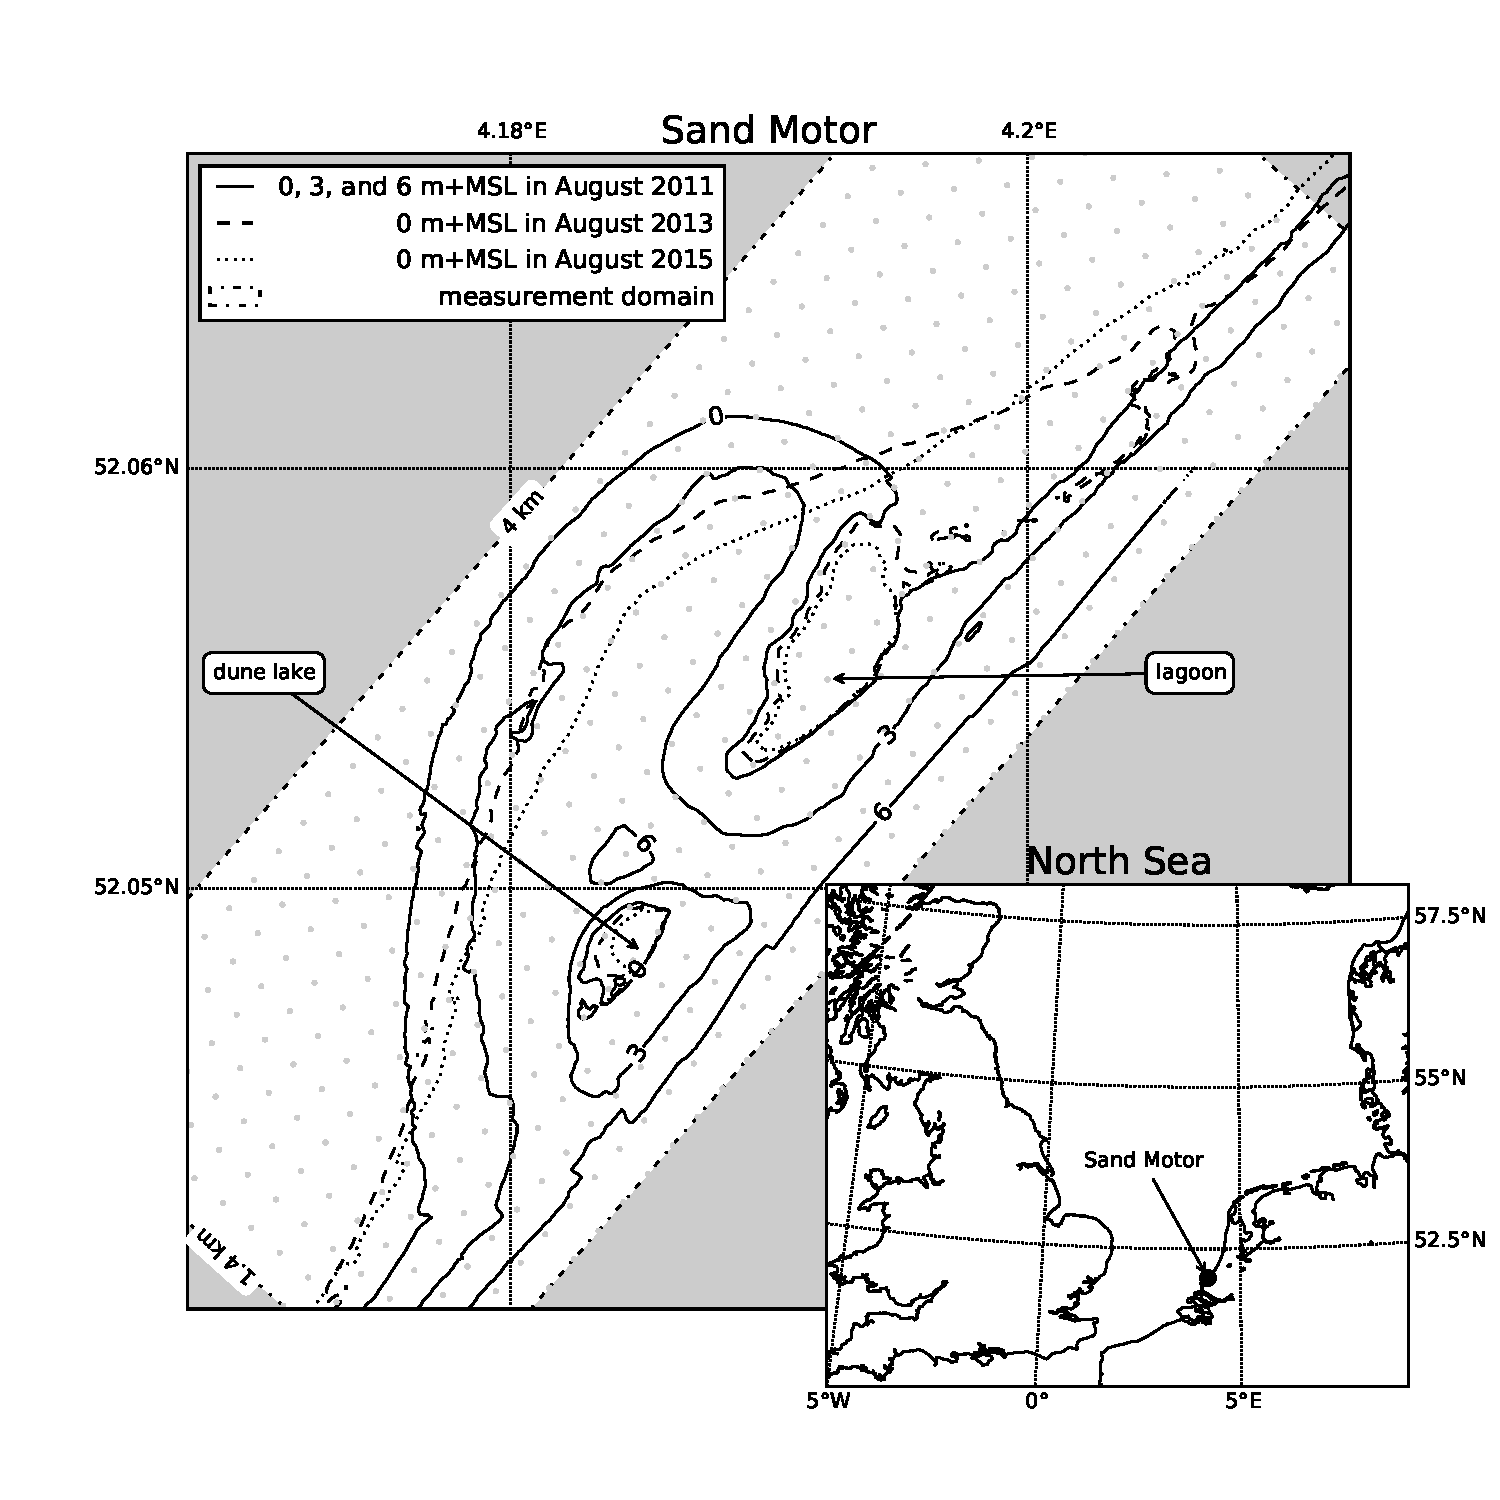
\includegraphics[width=\columnwidth]{../Figures/location_and_evolution}
  \caption{Location, orientation, appearance and evolution of the Sand
    Motor between construction 2011 and 2015. The box indicates the
    measurement domain used in the remainder of this paper. A 100 x
    100 m grid aligned with the measurement domain is plotted in gray
    as reference.}
  \label{fig:fieldsite2}
\end{figure}

Sand used for construction of the Sand Motor is medium sand with a
median diameter of about 350 $\mu \mathrm{m}$. The sand is obtained
from an offshore borrowing pit in the North Sea and contains many
shells and some pebbles, cobbles and other non-erodible material.

The predominant wind direction is south to southwest. Storms have a
tendency to be oriented either southwest or northwest. Also the
sediment transport potential ($\Psi$), defined as:

\begin{equation}
  \label{eq:transport_potential}
  \Psi \propto \int u^3 \mathrm{d}t
\end{equation}

\noindent in which $u$ is the wind speed, is predominantly
southwesterly or northwesterly oriented. The northwesterly storms are
generally accompanied with significant surges as the North Sea is
virtually unbounded in northwesterly direction (Figure
\ref{fig:fieldsite2}b).

The contour of the Sand Motor changed significantly in the four years
after construction. Tidal forces diffuse about 1 $\mathrm{Mm^3}$ per
year along the coast \citep{deSchipper2016}. Four years after
construction, the peninsula protrudes about 800 m into the sea and
stretches over 4 km alongshore (Figure \ref{fig:fieldsite2}).

%The tidal channel that connects the lagoon to the sea elongated and
%started to meander. Consequently, the 2 m tidal range that is present
%at the outer contour of the Sand Motor is damped over time to
%approximately 20 cm in the lagoon \citep{deVries2015}. At the closed
%end of the lagoon the tidal currents are therefore
%negligible. Consequently, morphological change in this area can be
%associated with aeolian sediment transport as is the morphological
%change in the dune lake.  The lagoon and dune lake therefore act as
%large sediment traps for aeolian sediment.

The Sand Motor provides a unique opportunity to perform measurements
on spatial variations in aeolian sediment availability and transport.
It accommodates vast and armored beaches next to dynamic intertidal
beaches of varying width, while limitations in fetch are negligible.

\section{Methodology}

Sediment transport measurements were performed to investigate the role
of the southern intertidal beaches as supplier of aeolian sediment in
the Sand Motor region \citep{Hoonhout2017a}. The change in sediment
transport in downwind direction (spatial gradient) was measured along
cross-shore transects running from the water line until the dry beach
at approximately 5 m+MSL. Spatial gradients in saltation transport are
positive in areas with net erosion and negative in areas with net
deposition of sediment. The measurements were performed
during the six week field campaign \textsc{MegaPEX} (Mega Perturbation
EXperiment) from September 17, 2014 until October 23, 2014.

\subsection{Equipment}

\begin{figure}
 \centering
  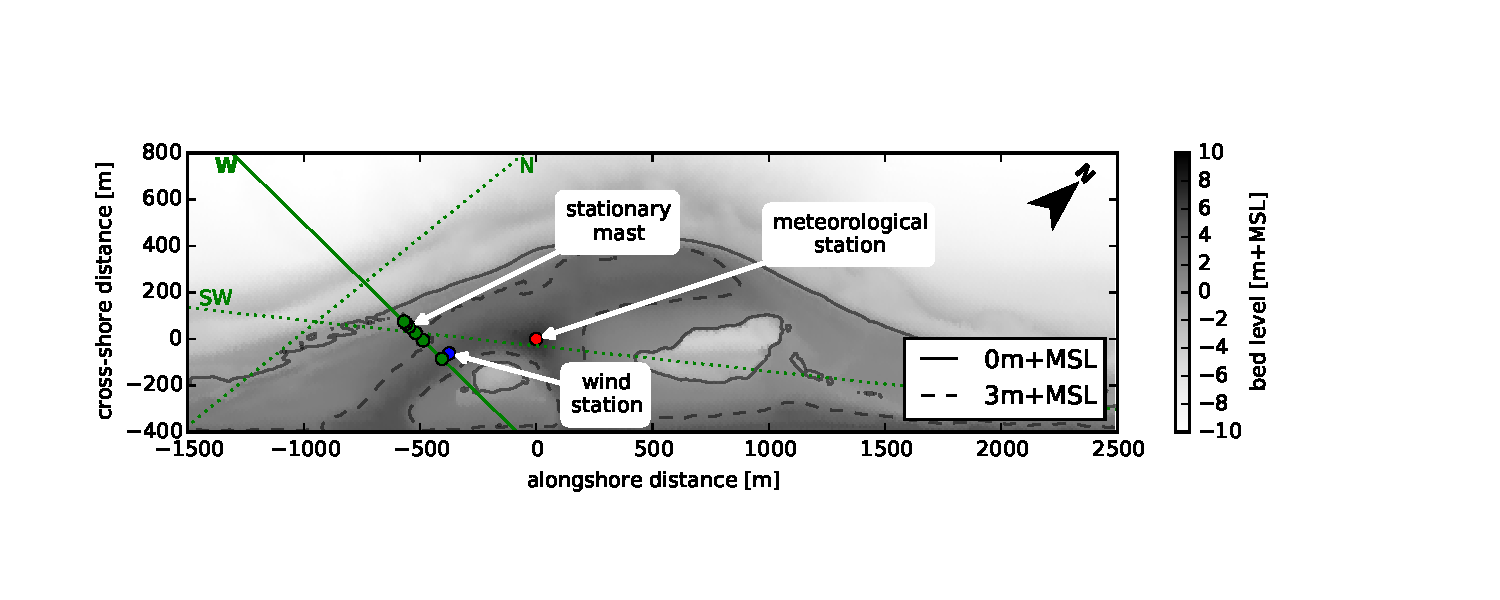
\includegraphics[width=\columnwidth]{../Figures/overview}
  \caption{Overview of measurement transects N, W, and SW and
    locations during the \textsc{MegaPEX} field campaign.}
  \label{fig:overview}
\end{figure}

\begin{figure}
 \centering
  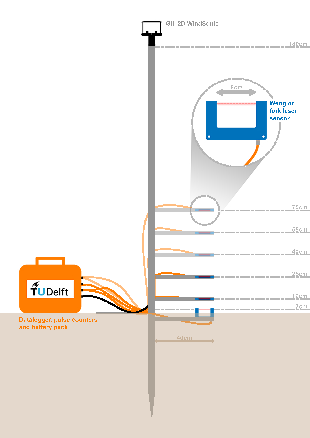
\includegraphics[width=\columnwidth]{../Figures/mast_small}
  \caption{Mast with 6 Wenglor fork laser sensors and a Gill 2D
    WindSonic ultrasonic wind speed and direction sensor viewed in
    direction of the wind. The top 3 laser sensors are optional.}
  \label{fig:mast}
\end{figure}

The measurement set-up consists of 8 masts with battery power and data
loggers. Each mast was equipped with at least three Wenglor fork laser
sensors (P/N: YH08PCT8) for saltation measurements at 3, 10 and 25 cm
above the bed (Figure \ref{fig:mast}). An additional three laser
sensors were added to the most landward mast at 40, 55 and 70 cm above
the bed to estimate the amount of particles bypassing the lower three
sensors. Other masts could be equipped with three additional laser
sensors as well. All except the lowest sensor were placed horizontally
with the arms directed towards the wind as to minimize the disturbance
of the wind field. The lowest sensor was placed vertically with the
arms directed upwards, and partially buried as to further minimize the
disturbance of the wind field. The Wenglor fork laser sensors register
passing particles of $50 ~ \mu \mathrm{m}$ and larger with a frequency
of 10 kHz using a laser beam of 0.6 mm. As the particle count is
linearly related to the sediment flux \citep{Hugenholtz2011}, both are
used indiscriminately in this study. The particle count is accumulated
by a HOBO pulse counter (P/N: S-UCC-M001). A HOBO Energy data logger
(P/N: H22-001) logged all sensors, including the pulse counters, at 1
Hz. In addition, three masts were equipped with a Gill 2D WindSonic
ultrasonic wind speed and direction sensor (P/N: 1405-PK-040) at a
height of 180 cm above the bed.

The masts can be rotated, but are not self-rotating to the wind as the
masts were relocated depending on the wind direction.  One stationary
mast was present during almost the entire field campaign (Figure
\ref{fig:overview}).

A separate Eijkelkamp wind station with three cup anemometers (P/N:
16.98.31) at heights 50, 100 and 180 cm and a wind vane (P/N:
16.98.34) at height 180 cm was present at a stationary location at the
high beach for the entire duration of the field campaign. A Campbell
Scientific meteorological station was present at the heart of the Sand
Motor providing measurements on precipitation, humidity, solar
radiation and wind speed and direction (Figure \ref{fig:overview}).

Qualitative small scale measurements on bed level change were
performed by pressing erosion pins (nails) in the beach with falling
tide. The erosion pins were placed along a cross-shore transect and
about 10 cm apart with their heads flush to the bed. The erosion
around the pins was measured manually with a ruler at the onset of
flood.

Daily topographic surveys are performed along cross-shore transects
using a Leica Viva GS10 RTG-GPS receiver. Offshore water levels and
wave heights are obtained from gauges at the permanent offshore
Europlatform.

\subsection{Deployments}

The measurement masts were deployed continuously during the field
campaign, but have been relocated according to the governing wind
direction. An overview of the measurement locations is given in Figure
\ref{fig:overview}. 

A single measurement transect consists of at least four masts: two in
the intertidal beach area in order to capture the entrainment rate
from the assumed sediment source region, one above the high water mark
to capture the sediment flux from the intertidal beach area onto the
dry upper beach and one higher up the beach to capture any additional
sediment supply from the dry beach itself. 

Table \ref{tab:deployments} lists the partitioning of the field
campaign in 10 deployments with constant location and orientation of
the measurement equipment. Most deployments were located along the
westerly transect at the southern flank of the Sand Motor (Figure
\ref{fig:overview}). Deployments DN02a and DN06a were aligned along
alternative transects concurrent with deployments DN02b and DN06b
respectively. During deployment DN11 all masts were clustered at high
grounds as to provide a safe buffer from the expected surge during the
storm event of October 23. Consequently, no transport gradients were
measured during deployment DN11.

\begin{table}[h]
  \centering
  \caption{Deployments of measurement masts during the \textsc{MegaPEX} field
    campaign. Maximum measured wind speeds are in parentheses.}
  \label{tab:deployments}
  \begin{tabular}[h]{lrrrrrrr}
    \hline
               & wind       &  wind      & laser      &   transect &   duration & sensors &     well \\
               & speed      & direction  & direction  &            &            &      &     oriented* \\
               &      [m/s] &     [$^o$] &     [$^o$] &            &        [h] &     [-] &       [\%] \\
    \hline
    DN02a      &     3 (10) &        358 &        262 &          W &         22 &       3 &          0 \\
    DN02b      &     3 (10) &        359 &        360 &          N &         22 &       3 &        100 \\
    DN04       &     5 (13) &        343 &        360 &          W &         42 &       3 &         92 \\
    DN05       &     3 (15) &        196 &        270 &          W &        312 &       3 &         40 \\
    DN06a      &     5 (17) &        166 &        225 &         SW &        170 &       3 &         55 \\
    DN06b      &     5 (17) &        180 &        225 &          W &        170 &       3 &         77 \\
    DN08       &     5 (16) &        199 &        225 &          W &        160 &       6 &         89 \\
    DN09       &     9 (21) &        240 &        270 &          W &         32 &       6 &         87 \\
    DN10       &    15 (22) &        301 &        315 &          W &          9 &       6 &        100 \\
    DN11       &    10 (24) &        322 &        315 &          - &         25 &       6 &         44 \\
    \hline
  \end{tabular}

  \footnotesize{
    \begin{enumerate}[{*}]
    \item The last column indicates the percentage of time in which
      the laser sensors were well oriented with respect to the wind.
      Raw data from all deployments is publishes as \citet{megapex}.
      DN01 is omitted from this list as it involved a test run of the
      equipment only. DN02a is listed only for convenience when
      interpreting the published dataset. DN02b and DN06b were
      originally named DN03 and DN07 respectively and can be found by
      these names only in the published dataset.
    \end{enumerate}}
\end{table}

\subsection{Data analysis}

Particle count time series obtained from individual Wenglor laser
sensors are summed up
\begin{enumerate}
\item per mast, to obtain \emph{per-mast} particle count time series
  for each measurement mast, and
\item over all masts, to obtain \emph{overall} particle count time
  series over all measurement masts.
\end{enumerate}
The per-mast particle counts are totaled rather than averaged, and
therefore not corrected for the number of Wenglor laser sensors per
mast. All masts deployed simultaneously in a single transect were
equipped with an equal number of sensors. Only the most landward mast
in the westerly transect was permanently equipped with six
sensors. However, the upper three sensors of the latter mast
registered negligible particle counts. Averaging would result in
approximately halving the per-mast particle counts. The halving of the
particle count does not reflect any physical behavior and is therefore
averted. Particle count time series are interchangeably referred to as
particle count rates as the measurement interval was 1 Hz.

The overall particle count time series are used for comparison with
the governing wind speed. For comparison with the wind direction
per-mast particle count time series are discretized in bins according
to the governing wind direction and subsequently summed over
time. Also for comparison with water and bed levels, the per-mast
particle count time series are discretized in bins and summed over
time. Discretization is then done according to the global water level
and local bed level at the measurement location.

Horizontal gradients in particle counts are computed from the per-mast
particle count time series and the distance between the measurement
masts. Vertical distributions in particle counts are computed from the
per-sensor particle count time series for each measurement mast.

Particle counts are converted into sediment fluxes following
\citet{Barchyn2014}:

\begin{equation}
  q_{\mathrm{wenglor}} = n_{\mathrm{wenglor}} \left( 
    \frac{6 \cdot \gamma}{\rho \pi D^3} \cdot l_{\mathrm{fork}} \cdot \left(
      l_{\mathrm{laser}} + D \right) \right)^{-1}
\end{equation}

\noindent with $\rho = 2650$ $\mathrm{kg/m^3}$,
$l_{\mathrm{fork}} = 8 \cdot 10^{-2}$ m,
$l_{\mathrm{laser}} = 6 \cdot 10^{-4}$ m, $D = 335$ $\mathrm{\mu m}$
and $\gamma = 1$.

Variations in wind direction of more than $45^o$ resulted in
adjustment of the orientation of the Wenglor fork laser
sensors. Particle counts with a discrepancy between wind direction and
laser orientation ($\Delta \theta_u$) of more than $60^o$ are
considered not well oriented and are discarded from the presented
analysis. Other particle counts ($n_{\mathrm{pc}}$) are corrected for
orientation inaccuracies ($\hat{n}_{\mathrm{pc}}$) using the basic
geometric correction:

\begin{equation}
  \hat{n}_{\mathrm{pc}} = \frac{n_{\mathrm{pc}}}{\cos(\Delta \theta_u)}
\end{equation}

Periods without significant particle counts are not discarded from the
analysis, except for the determination of the average wind direction
as the wind direction tends to show random behavior for low wind
conditions. The last column in Table \ref{tab:deployments} states the
percentage of time in the laser sensors were well oriented with
respect to the wind direction.

\section{Results}

\begin{figure}
 \centering
  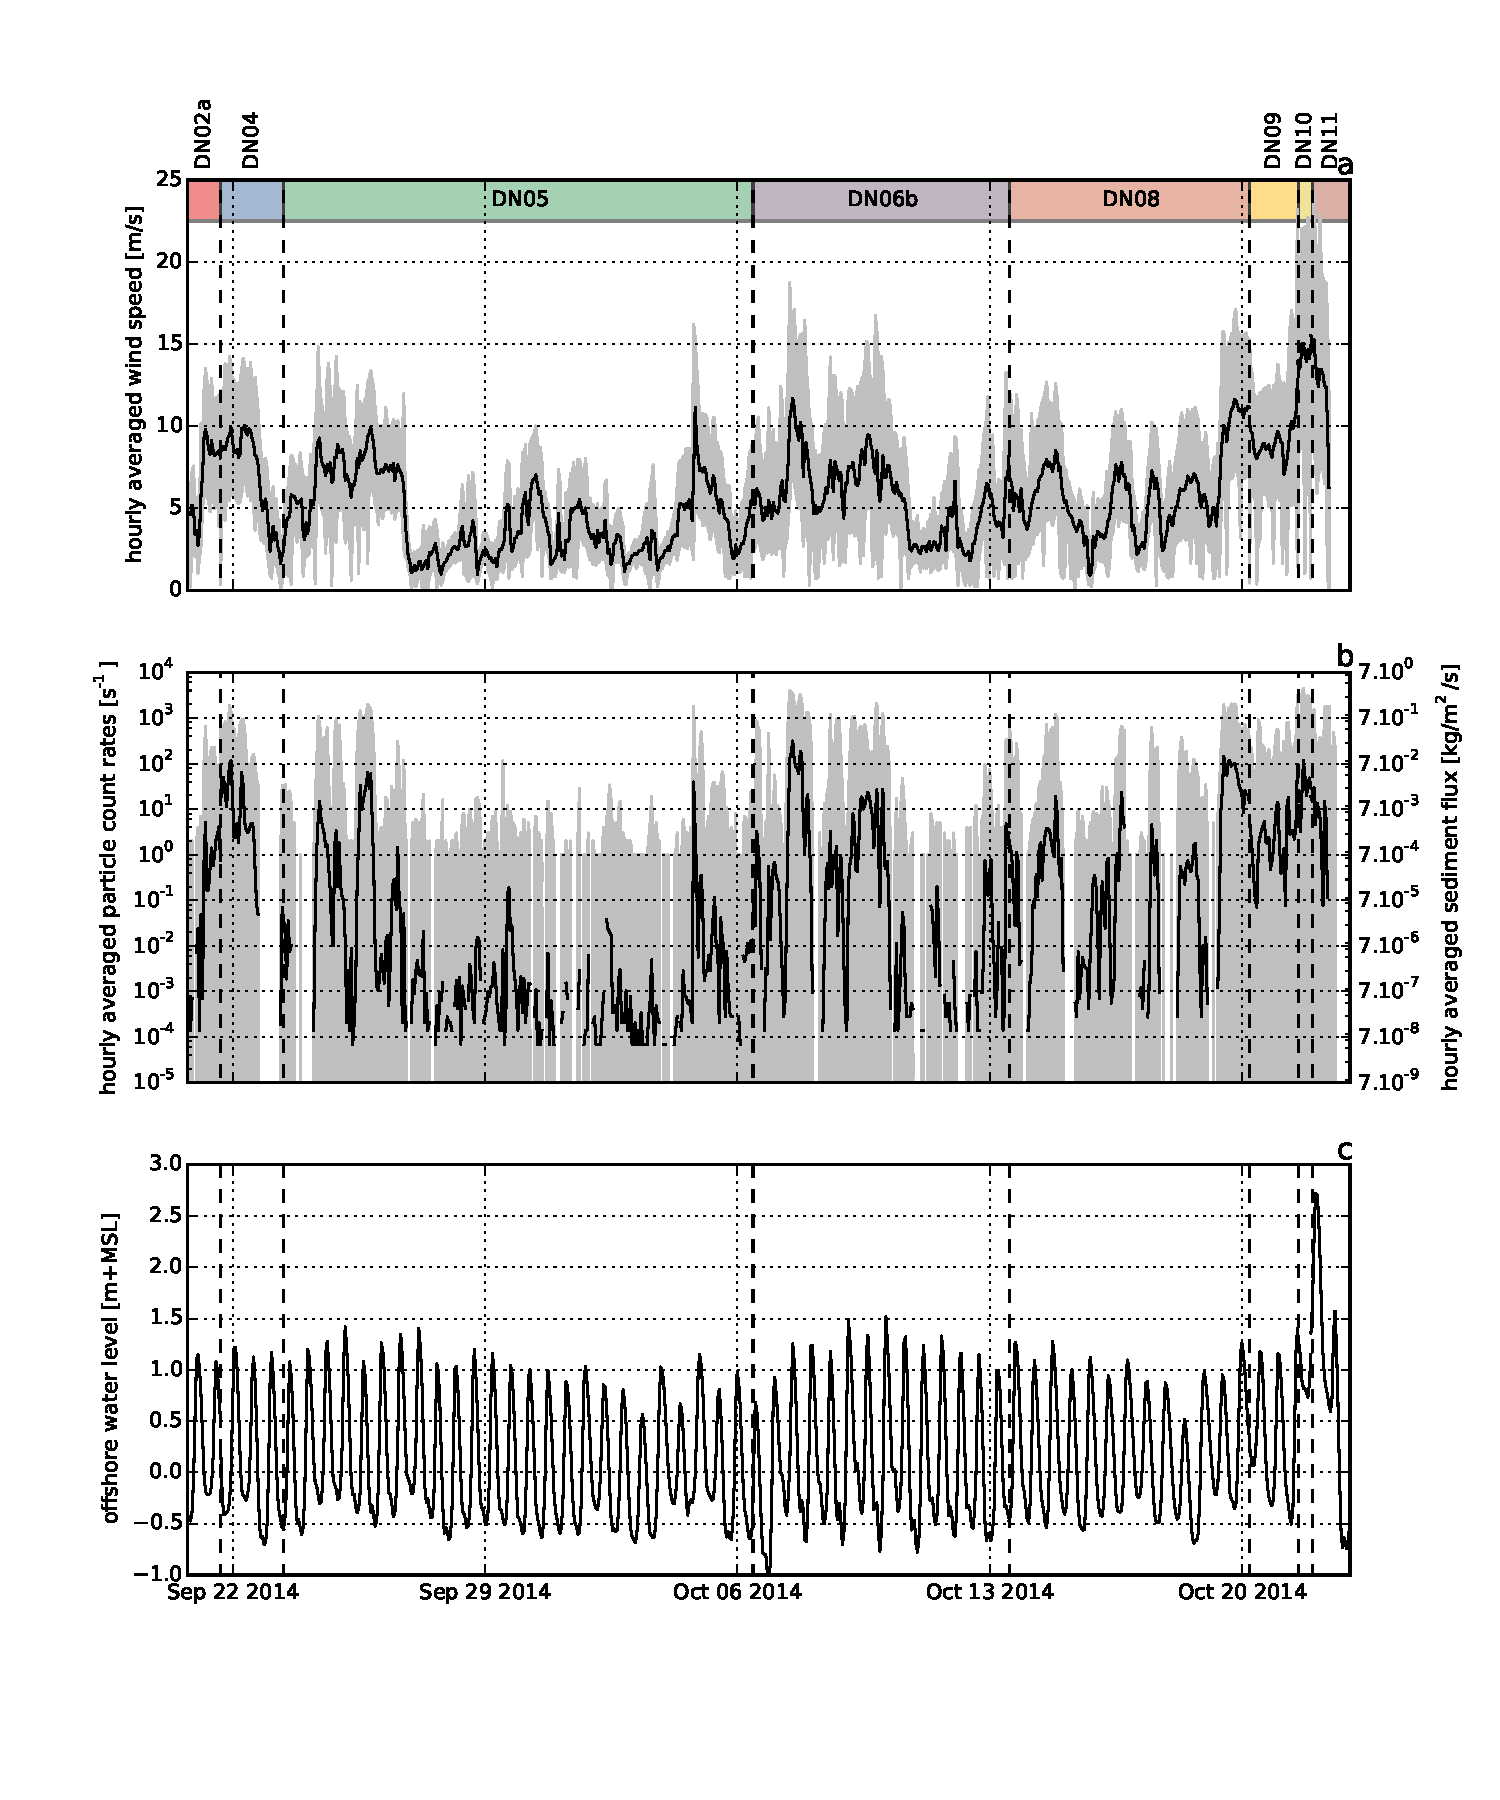
\includegraphics[width=\columnwidth]{../Figures/particlecounts_timeseries}
  \caption{a) Wind time series, b) overall particle count rates during
    the deployments along the westerly transect, and c) offshore tidal
    elevation. Grey lines indicate the raw data, black lines the
    hourly averaged data. Colored bars refer to the deployments listed
    in Table \ref{tab:deployments}. Deployments DN02b and DN06a are
    not included as these are located along different transects.}
  \label{fig:pc_timeseries}
\end{figure}

\begin{figure}
 \centering
  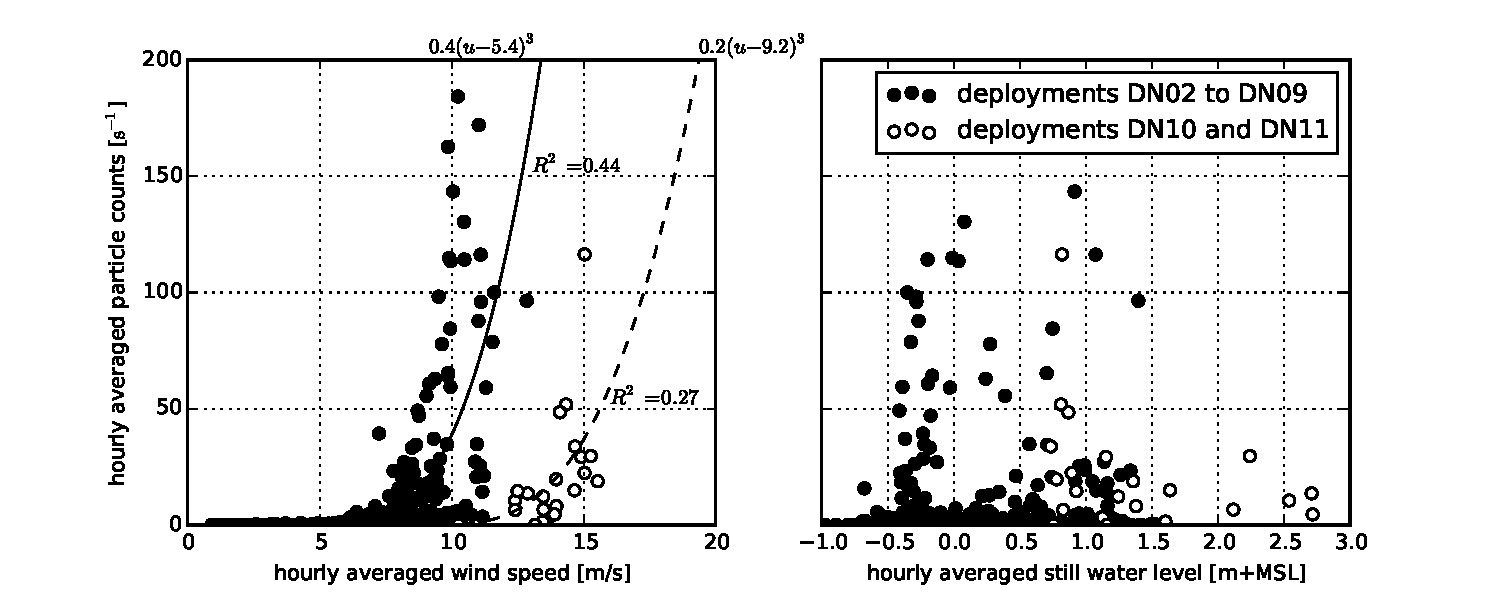
\includegraphics[width=\columnwidth]{../Figures/particlecounts_correlations}
  \caption{a) Relations between overall particle count and wind speed
    or b) water level. Closed circles and continuous lines refer to
    non-storm deployments DN02 to DN09. Open circles and dashed lines
    refer to storm deployments DN10 and DN11. All deployments are
    listed in Table \ref{tab:deployments}.}
  \label{fig:pc_correlations}
\end{figure}

The conditions during the field campaign were characterized by calm
and sunny weather and negligible precipitation, which is unusual for
the time of the year. The average wind speed over the entire
experiment was 6 m/s (Figure \ref{fig:pc_timeseries}a). The maximum
wind speed was registered at 24 m/s at the end of the campaign on
October 23 during the only measured storm event (DN10). The average
overall particle count rate over the entire experiment was 120
$\mathrm{s^{-1}}$ or $< 0.1$ $\mathrm{kg/m^2/s}$ averaged over all
deployed sensors (Figure \ref{fig:pc_timeseries}b). The maximum
overall particle count rate was registered on October 7 at 5800
$\mathrm{s^{-1}}$ or 4 $\mathrm{kg/m^2/s}$ (DN06b). Therefore, the
maximum registered overall particle count rate did not coincide with
the maximum wind speed.

The experiment covered two spring-neap cycles with a tidal range
varying between 1.5 and 2.0 m (Figure \ref{fig:pc_timeseries}c). The
maximum still water level of 2.8 m+MSL was measured during storm
deployment DN11 on October 22. This surge flooded the southern flank
of the Sand Motor up to 5 m+MSL.

\subsection{Relation between sediment transport and wind speed and
  water level}

Periods with low wind conditions seem to coincide with periods with a
negligible overall particle count, whereas periods with fair wind
conditions seem to coincide with periods with a significant overall
particle count (Figure \ref{fig:pc_timeseries}a,b). Also the
occurrence of peaks in overall particle count show a correspondence
with peaks in wind speed. However, the highest peaks in wind speed do
not necessarily coincide with the highest peaks in overall particle
count, resulting in an overall poor correlation between wind speed and
overall particle count (Figure \ref{fig:pc_correlations}a). The poor
correlation is reflected in a Spearman rank correlation coefficient
\citep{Spearman1904} of zero, indicating that the data cannot be
described by a monotonic function of any kind.

In the remainder of this paper it is shown that the storm deployments
DN10 and DN11 provide signals with respect to wind direction, sediment
availability and fetch that are consistently different from the
non-storm deployments DN02 to DN09. In anticipation to these findings,
correlations between wind speed and overall particle count are
computed for the storm and non-storm deployments separately, resulting
in a weak positive relation between wind speed and overall particle
count. Fitting a third-power curve through these separate datasets
results in $R^2$-values of 0.43 and 0.27 respectively. The low
$R^2$-values indicate that much of the variance in the overall
particle count is not explained by wind speed.

No relation between the still water level and the overall particle
count is found (Figure \ref{fig:pc_correlations}b). There is no
evidence that the spring-neap modulation of the high water level of
about 0.5 m influenced the overall particle count significantly.

\subsection{Wind direction and sediment source areas}

\begin{figure}
 \centering
  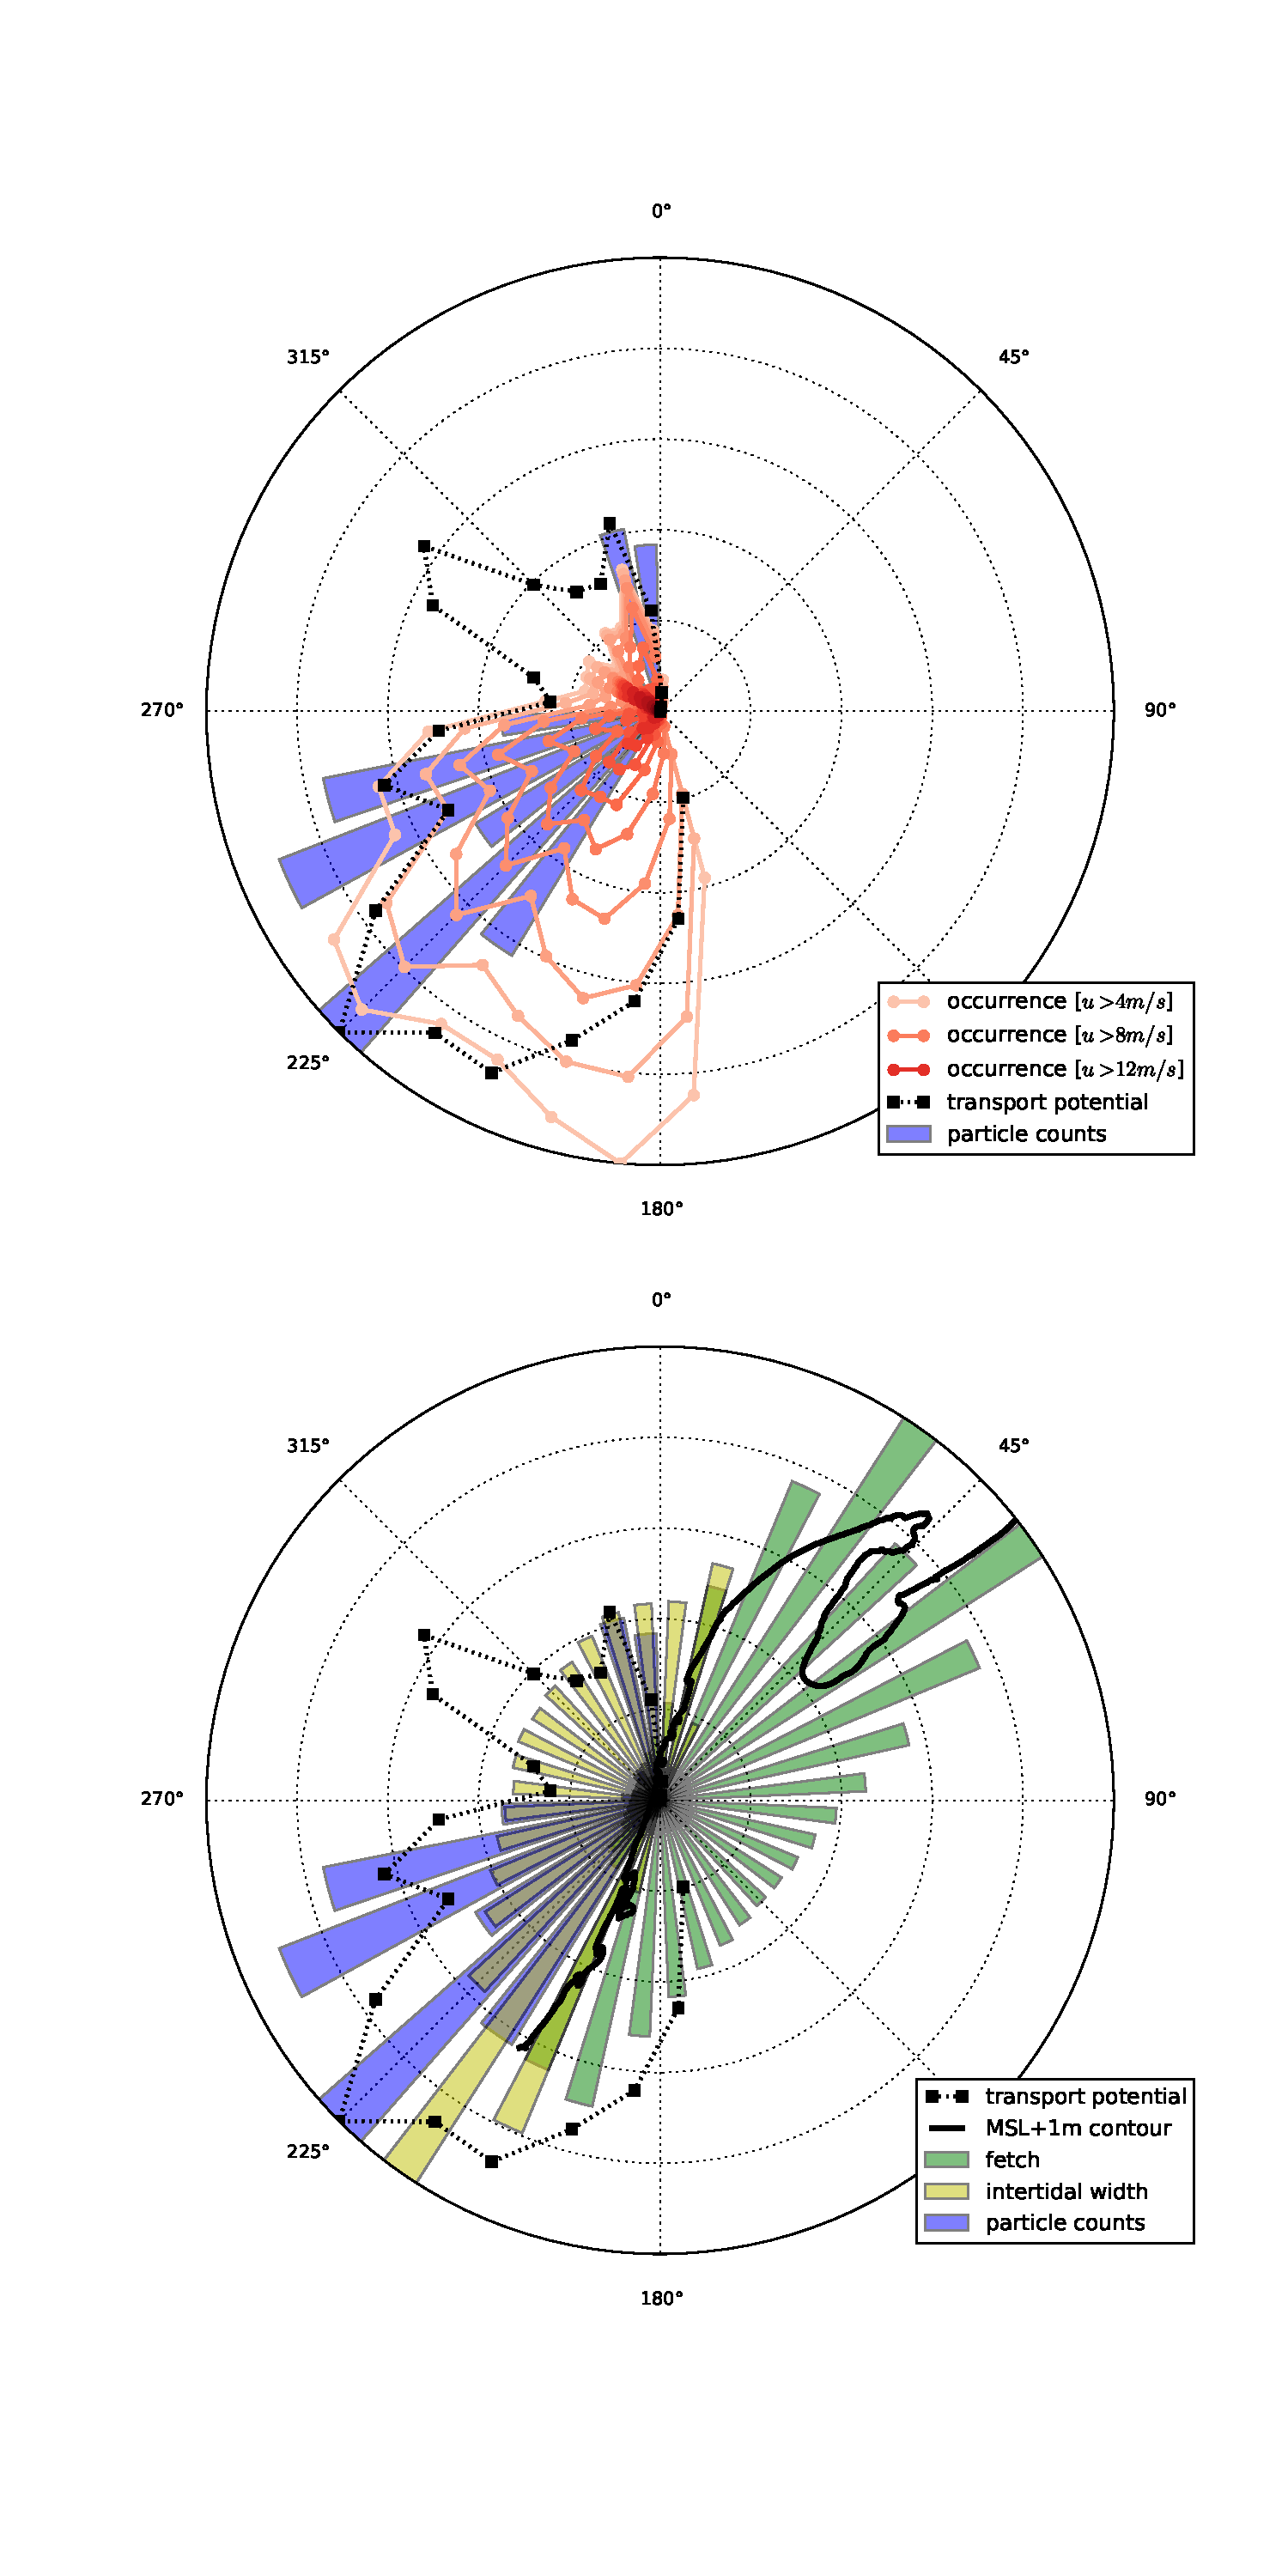
\includegraphics[width=.7\columnwidth]{../Figures/polar_72096_451703}
  \caption{a) Per-mast particle count, wind speed and direction
    obtained from stationary mast (Figure \ref{fig:overview}) and b)
    available fetch and intertidal fetches.}
  \label{fig:pc_direction}
\end{figure}

The vast majority of per-mast particle counts registered at the
stationary mast, that was located at the high water line during almost
the entire field campaign (Figure \ref{fig:overview}), was registered
from a limited number of wind directions. These directions do not
coincide with the prevailing wind direction or the wind direction with
the largest transport potential (Figure \ref{fig:pc_direction}a).

Figure \ref{fig:pc_direction}a shows that the prevailing wind
direction was south, but that the largest transport potential
(Equation \ref{eq:transport_potential}) came from the southwesterly
and northwesterly directions. The per-mast particle count does not
align with the prevailing wind direction or the directions with the
largest transport potential as both the southerly and northwesterly
wind directions did not induce a significant particle count.

Figure \ref{fig:pc_direction}b shows that most particles are
registered from the wind directions with the shortest
fetches. However, these wind directions provide among the largest
intertidal beach widths along the Dutch coast. The exception is the
northwesterly wind direction, that does accommodate a fair intertidal
beach width, but did not register a per-mast particle count close to
what could be expected from the transport potential. The northwesterly
wind directions were solely present during the storm deployment DN10.

\subsection{Spatial gradients in sediment transport}

\begin{figure}
 \centering
  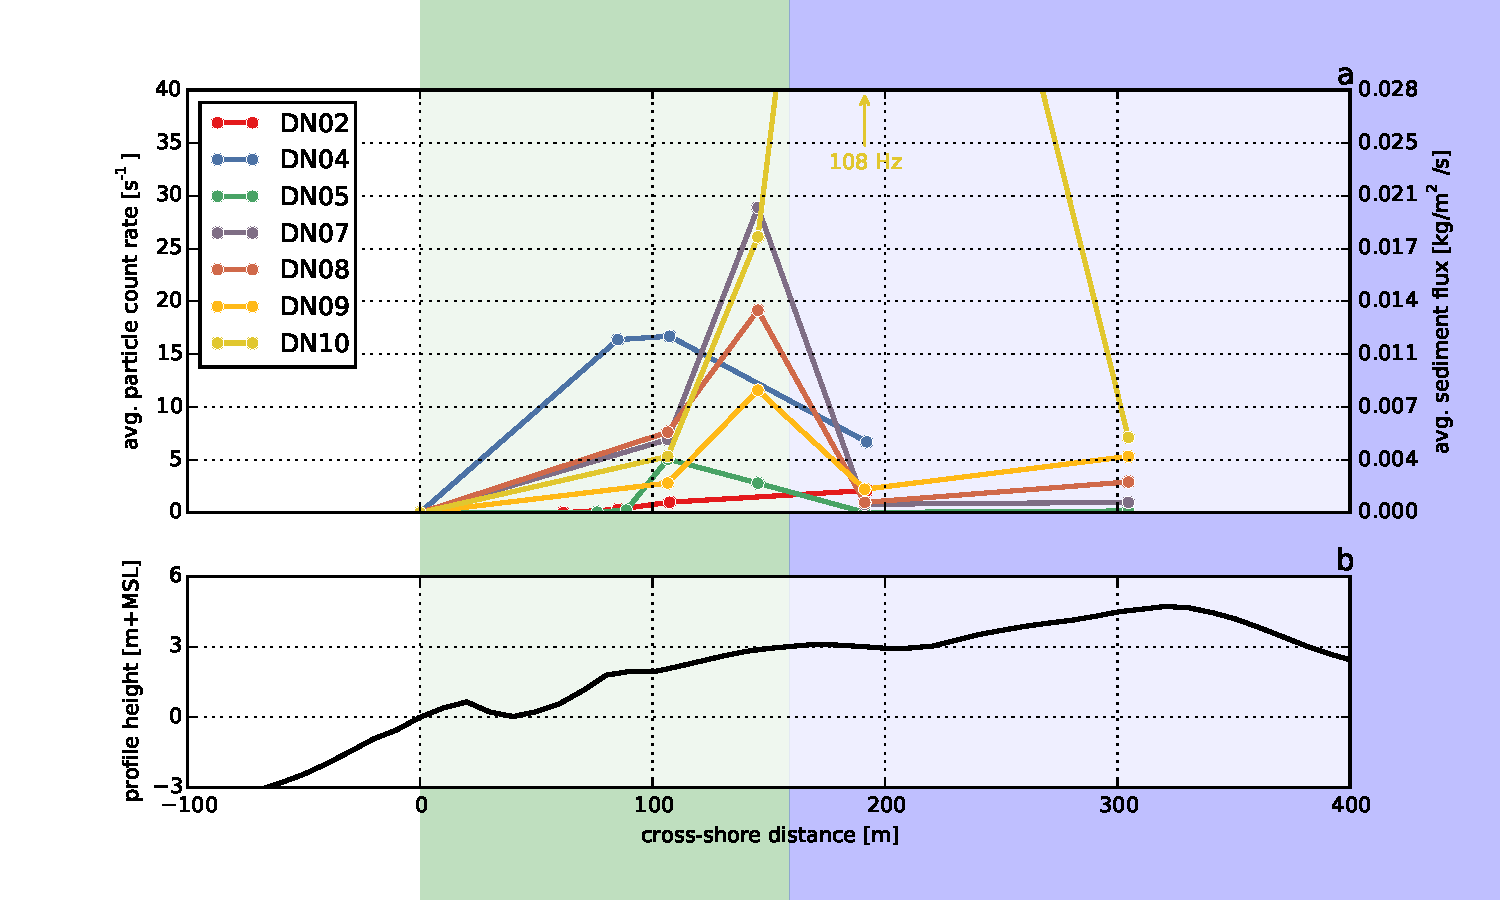
\includegraphics[width=\columnwidth]{../Figures/particlecounts_transects}
  \caption{a) Average per-mast particle count rates during the
    deployments along the westerly transect and b) beach profile at
    the beginning of the field campaign. Line colors refer to the
    partitioning of the time series in Figure
    \ref{fig:pc_timeseries}.}
  \label{fig:pc_transect}
\end{figure}

\begin{figure}
 \centering
  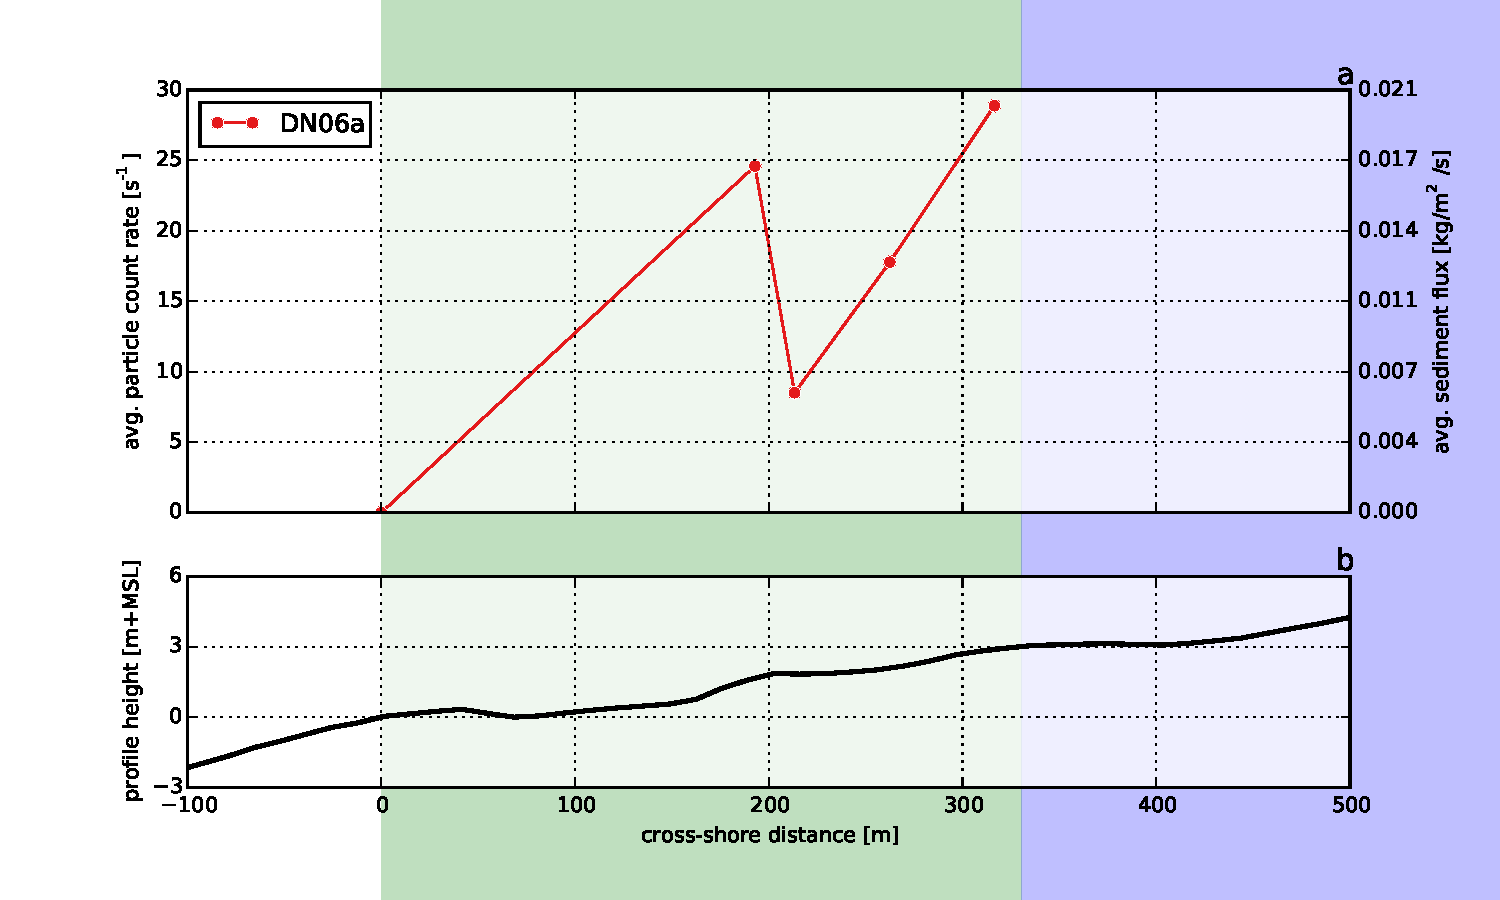
\includegraphics[width=\columnwidth]{../Figures/particlecounts_DN06}
  \caption{a) Average per-mast particle count rates during deployment
    DN06a along the southwesterly transect and b) beach profile at the
    beginning of deployment DN06.}
  \label{fig:pc_transect_DN06}
\end{figure}

\begin{figure}
 \centering
  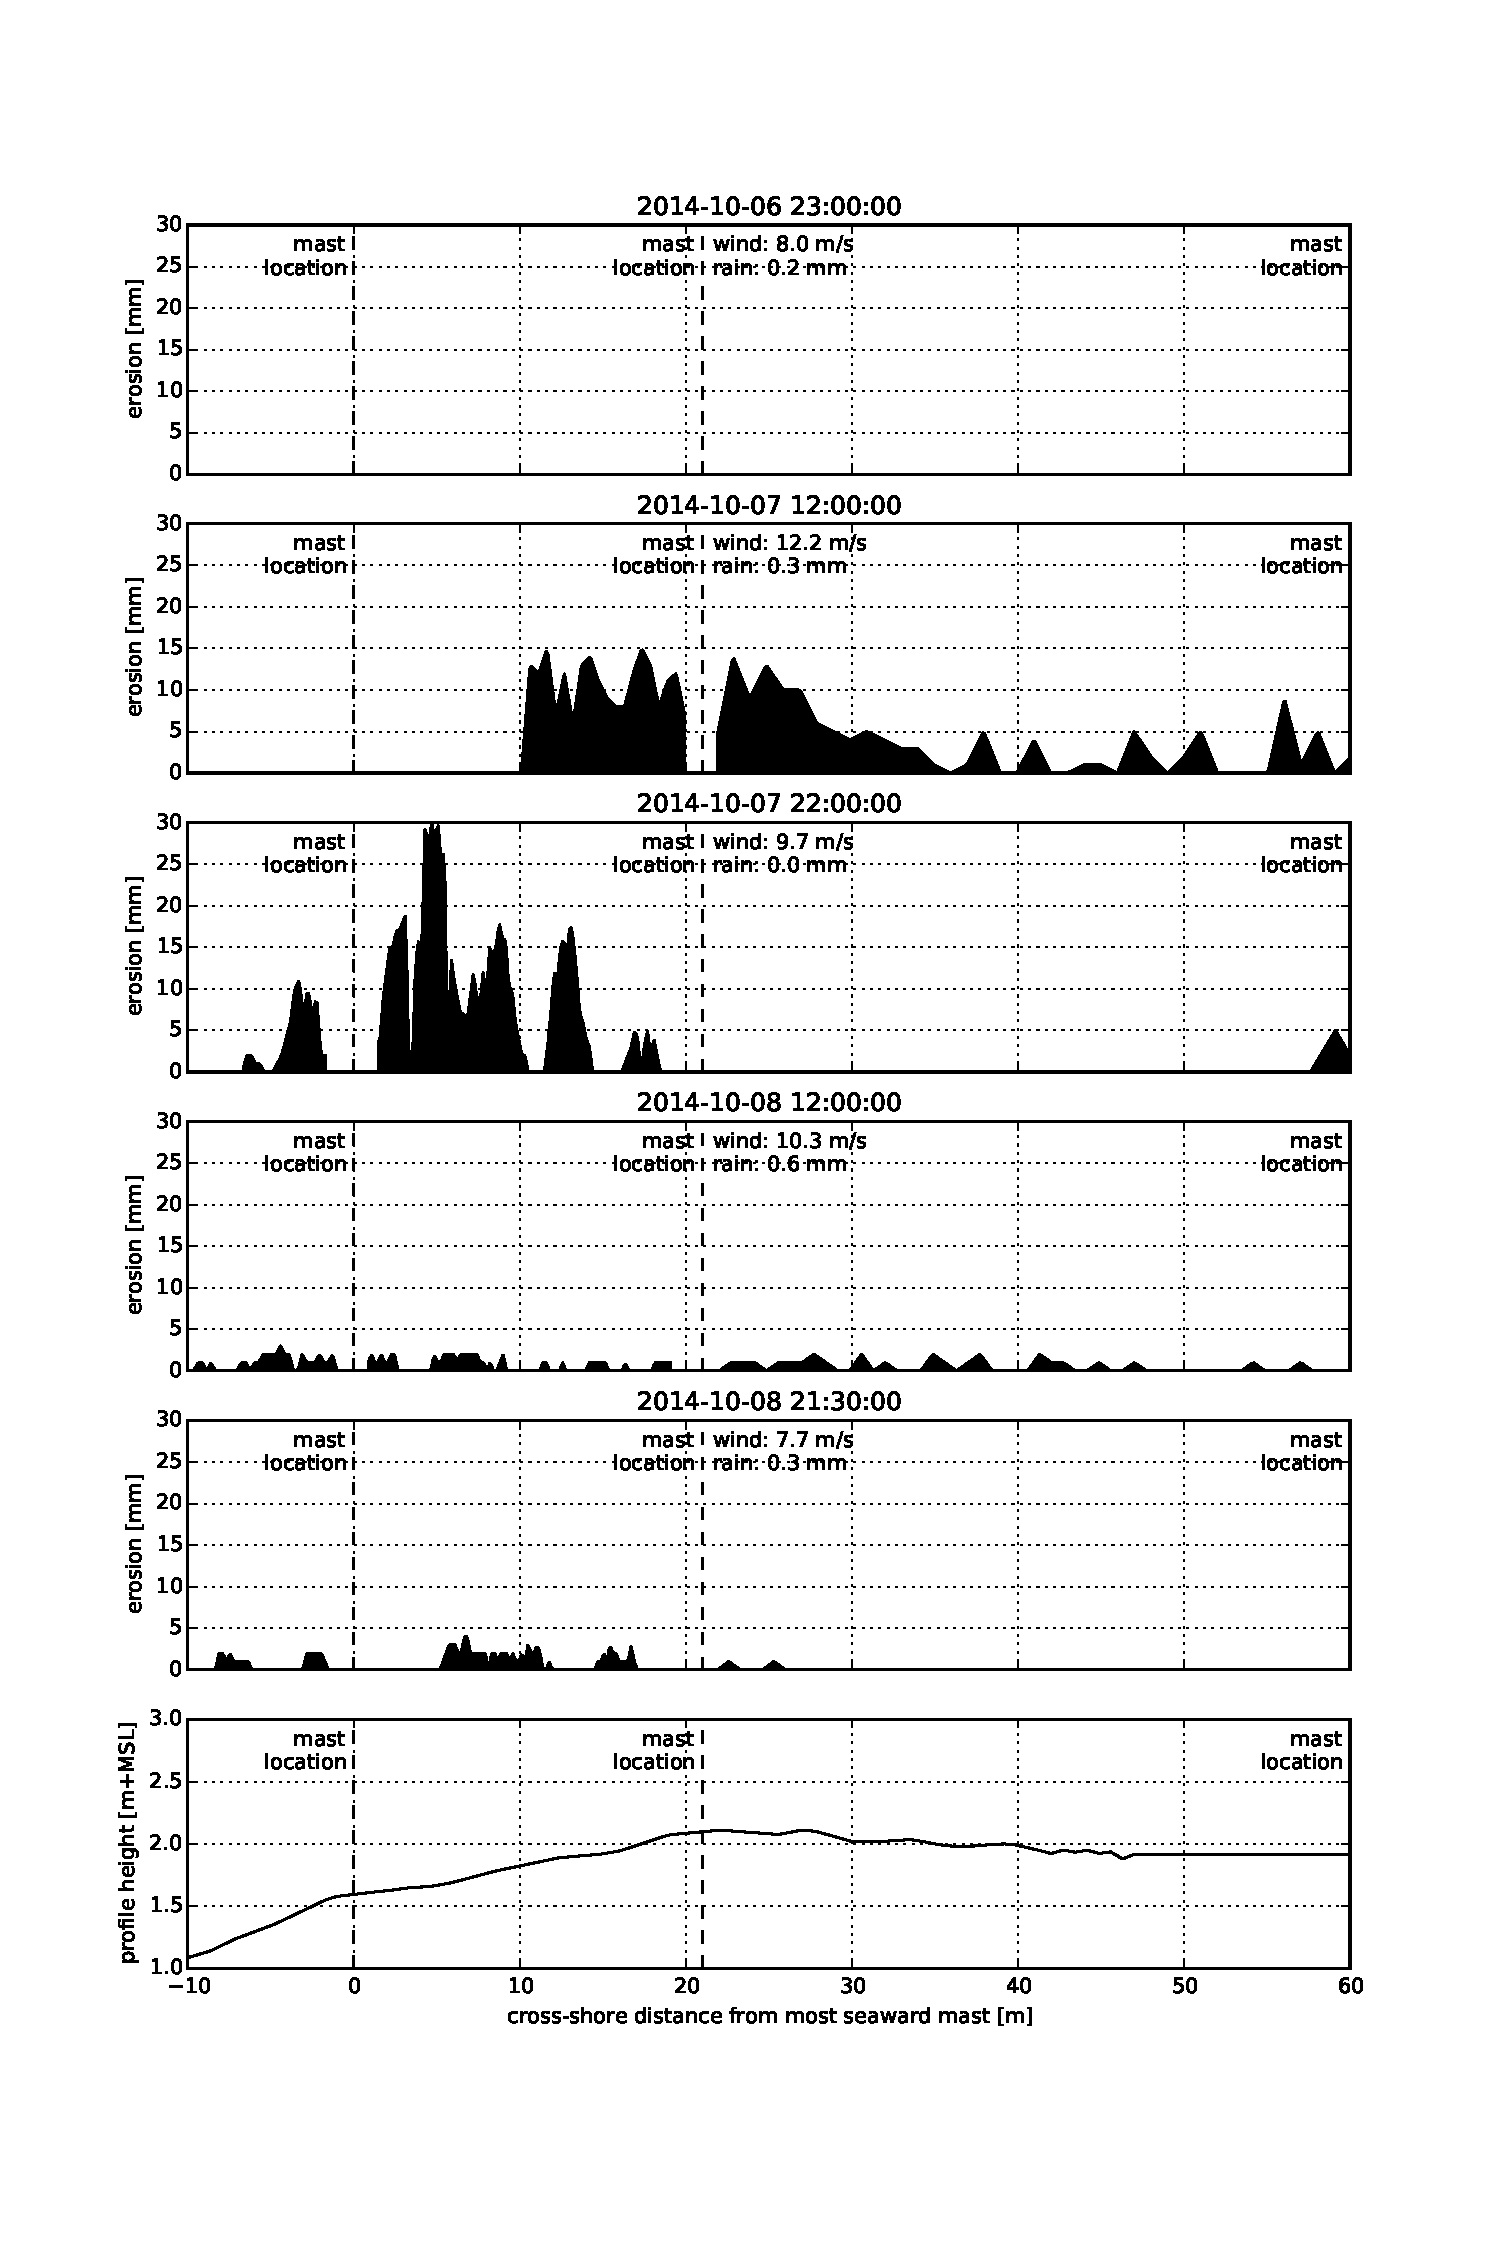
\includegraphics[width=\columnwidth]{../Figures/nails}
  \caption{Erosion measured using erosion pins during five tidal
    cycles during deployment DN06a along the southwesterly transect.}
  \label{fig:nails}
\end{figure}

Significant variations in per-mast particle count along the
measurement transects is found. Figure \ref{fig:pc_transect} shows
that the largest increase in per-mast particle count in downwind
direction (positive gradients) is consistently located in the
intertidal beach area. Positive gradients in sediment transport
indicate a net erosion of the beach surface and thus entrainment of
sediment.
% The positive gradients in the intertidal beach area therefore suggest
% that the intertidal beach is an important source of aeolian
% sediment. The small positive gradients over the dry beach similarly
% suggest that this area is a minor source of sediment.

A significant decrease in per-mast particle count in downwind
direction (negative gradients) is consistently found at the transition
between intertidal and dry beach. Negative gradients in sediment
transport indicate net deposition of sediment. Only during storm
deployment DN10 the negative gradients at the transition were absent
and large positive gradients in both the intertidal and dry beach area
were found (Figure \ref{fig:pc_transect}).
% The negative gradients therefore indicate that deposition of sediment
% occurs locally at the transition between intertidal and dry beach.

The negative gradients coincide with the transition from the berm
slope to the berm flat. Local deposition of aeolian sediment at the
edge of a berm appears to be consistent behavior as it is also
observed within the intertidal beach area. Four masts were deployed
along a southwesterly transect within the intertidal beach area
(DN06a, Figure \ref{fig:pc_transect_DN06}) concurrent with deployment
DN06b. These measurements show a significant decrease in per-mast
particle count over a minor berm-like feature (x = 200 m) in the
intertidal beach area. Downwind of this feature the per-mast particle
count increased again with a rate comparable to what was found upwind
of the berm-like feature. In addition, small scale measurements on bed
level change confirm that erosion by wind is concentrated on the berm
slope (Figure \ref{fig:nails}), while the berm flat tends to
accrete. The maximum erosion of 1.2 cm in a single tidal cycle was
measured with wind speeds above 10 m/s and little precipitation.

\begin{figure}
 \centering
  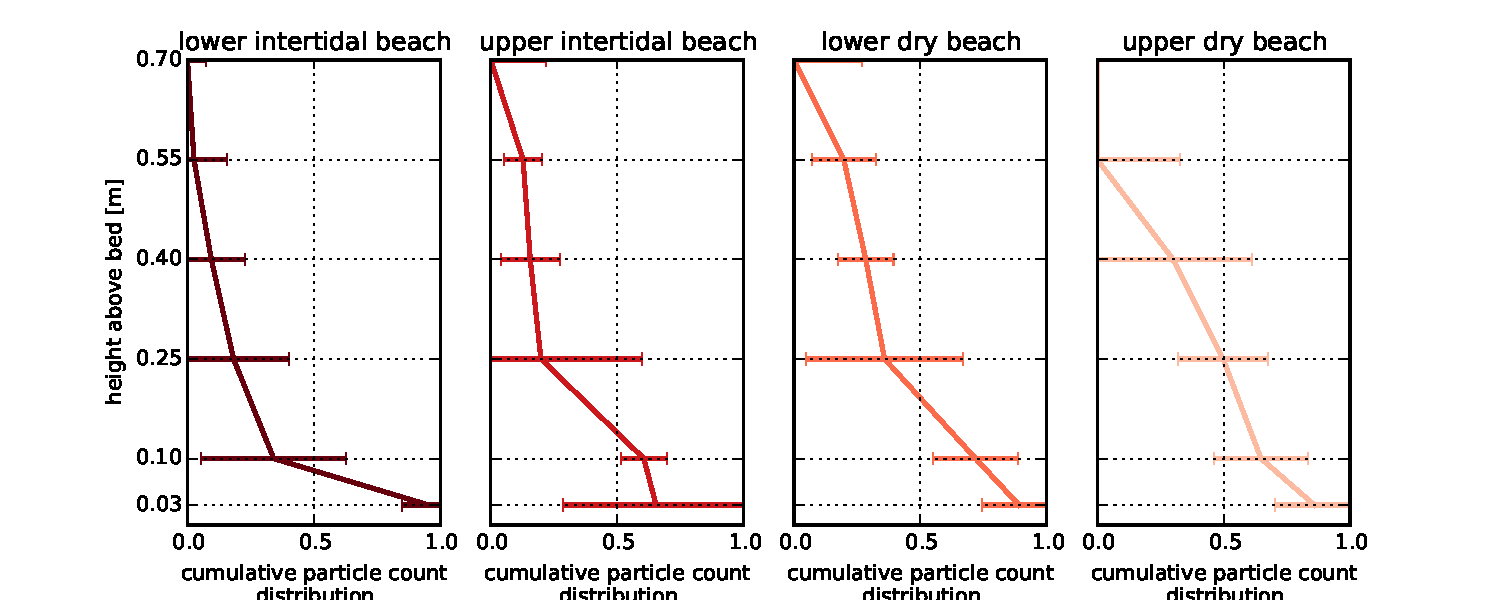
\includegraphics[width=\columnwidth]{../Figures/particlecounts_distheight}
  \caption{Cumulative particle count distribution over the vertical
    during deployment DN08. The line indicates the percentage of
    particles that bypasses a certain height above the bed. The
    horizontal bars visualize the variability in time of the particle
    count per laser sensor.}
  \label{fig:pc_distheight}
\end{figure}

Measured negative gradients might also be caused by sediment locally
bypassing the measurement equipment. To ensure that the number of
bypassing particles is limited, the most landward mast in each
transect was permanently equipped with six laser sensors up to 70 cm
above the bed. The number of particles counted in the upper laser
sensor was consistently low ($\leq 1\%$), suggesting that only a small
number of particles bypassed the equipment at this point.

At the location downwind of the negative gradients more sediment might
have bypassed than at the most landward measurement location. During
deployment DN08 all four masts were equipped with six laser sensors in
order to capture the vertical distribution of the particle count
across the beach (Figure \ref{fig:pc_distheight}). It appears that the
center of gravity of the particle count moves upward in downwind
direction.%, which seems in accordance with the development of a
%boundary layer
Downwind of the negative transport gradient the
percentage of particles counted by the upper laser sensor is 20\%
compared to $\leq 10\%$ at the other locations, suggesting that most
particles bypassed at this location. The difference between the
fraction of bypassing particles is too small to explain the large
negative gradients, but are likely to cause the measured negative
gradients to be overestimated.

\subsection{Fetch vs. sediment availability}

\begin{figure}
 \centering
  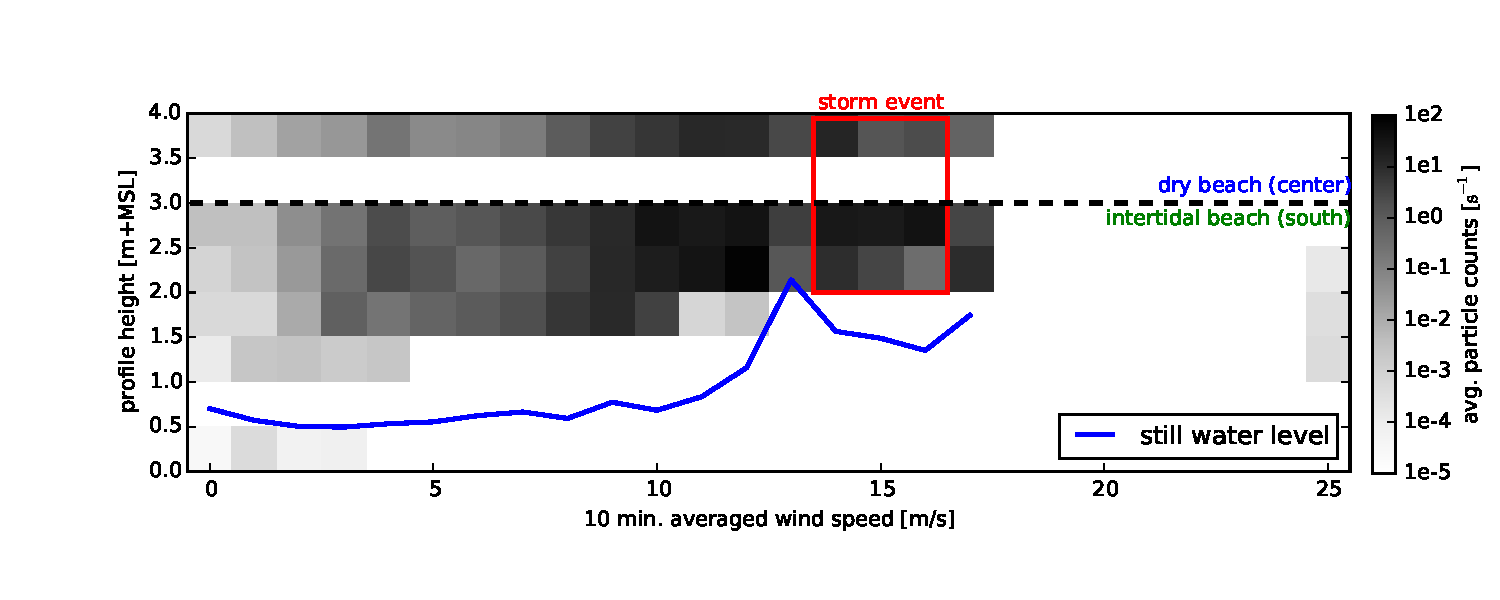
\includegraphics[width=\columnwidth]{../Figures/particlecounts_velocities}
  \caption{Average overall particle count rates depending on governing
    wind speed and bed level at measurement location, and average
    still water level depending on governing wind speed.}
  \label{fig:pc_velocity}
\end{figure}

In Figure \ref{fig:pc_velocity} the overall particle count obtained
during the field campaign is binned according to the prevailing wind
speed and the bed level at the measurement location. The average still
water level is an indication of available fetch. The peak in overall
particle count is at 3 m+MSL irrespective of the wind speed and
available fetch. Therefore the overall particle count seems to be
limited by location rather than wind speed or available fetch. The
specific location at which the particle count peaks corresponds to the
high water line and the onset of the shell pavement that largely
covers the dry beach.

\section{Discussion}

% positive gradients
The positive gradients in per-mast particle count in the intertidal
beach area and minor positive gradients in the dry beach area suggest
that the intertidal beach is a primary source of aeolian sediment in
the Sand Motor region. This observation is in accordance with the
large scale sediment budgets of the Sand Motor region
\citep{Hoonhout2017a}. Armoring of the dry beach surface, due to
formation of lag deposits, might lead to a significant reduction in
local aeolian sediment availability. Similarly, sediment availability
might also be limited in the intertidal beach area due to periodic
flooding and consequently high soil moisture contents. From the
differences in per-mast particle count gradients between the
intertidal and dry beach it can be assumed that the reduction of
sediment availability due to armoring outweighs the influence of soil
moisture. Local differences in bed surface properties would therefore
induce relative differences in sediment availability that govern
aeolian sediment transport in the Sand Motor region.

\begin{figure}
  \centering
  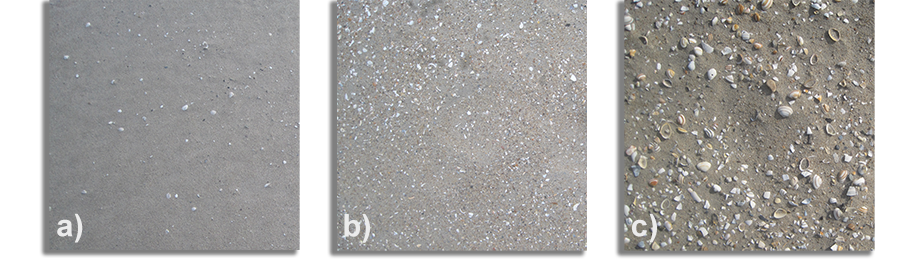
\includegraphics[width=\columnwidth]{../Figures/armoring_small}
  \caption{Visual impression of armor layer at three locations in the
    Sand Motor region: a) intertidal beach, no armoring b) lower dry
    beach, minor armoring with shell fragments c) upper dry beach,
    severe armoring with many shells and coarse sand. Covered surface
    is approximately 40 x 40 cm in all cases.}
  \label{fig:armoring}
\end{figure}

% negative gradients
The negative gradients in per-mast particle count at the transition
between intertidal and dry beach indicate that sediment eroded from
the intertidal beach is deposited locally on the dry
beach. Morphological feedback with the wind might cause the sediment
transport capacity to peak at the berm edge due to the presence of a
locally accelerated wind \citep[i.e. jet flow;][]{Hesp2016}, resulting
in deposition at the berm flat. In addition, the berm edge coincides
with the visually observed onset of a shell pavement (Figure
\ref{fig:armoring}). The shell pavement emerged from the nourished
sediment in the first half year after construction of the Sand Motor
\citep{Hoonhout2017a} due to winnowing of sand from the bed. Roughness
elements, like shells and cobbles, might trap impacting grains, and
hamper saltation, or cause fully elastic collisions, and enhance
saltation. The shell pavement at the measurement locations is
relatively open and therefore both processes are likely to be
relevant. The consistent negative gradients in particle count at the
onset of the shell pavement suggest that trapping of sediment is
dominant over the enhancement of saltation due to fully elastic
collisions.

% local storage and correlation water levels
\begin{figure}
 \centering
  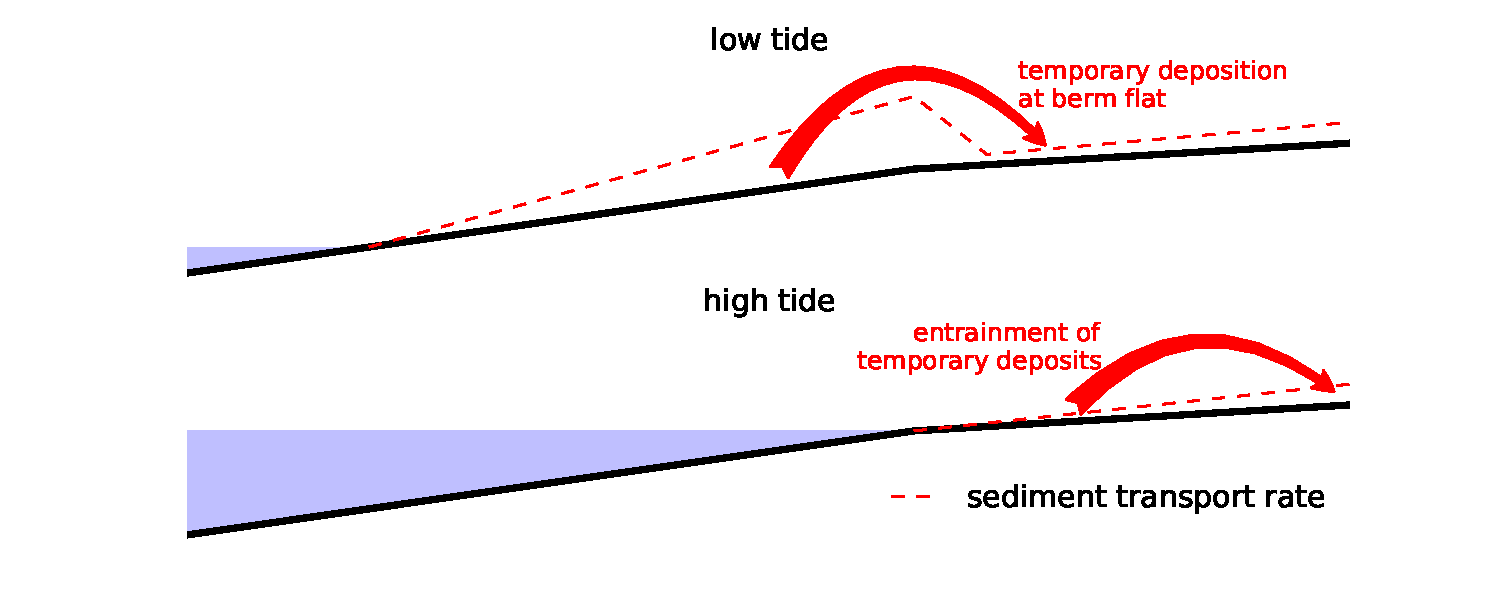
\includegraphics[width=\columnwidth]{../Figures/temporal_deposits}
  \caption{Conceptual illustration of how temporal deposits facilitate
    a continuous sediment supply from the intertidal beach to the
    dunes.}
  \label{fig:temporal_deposits}
\end{figure}

The local deposition of sediment at the berm flat is temporary as no
accumulation of sand is observed on top of the shell pavement during
the \textsc{MegaPEX} field campaign. This suggests that sediment
supply from marine sources and deposition in dunes, dune lake and
lagoon is a phased process. In a phased system the local sediment
deposits at the berm flat might act as temporary sediment source
during high water (Figure \ref{fig:temporal_deposits}). Consequently,
measured aeolian sediment transport rates would be continuous and
independent of the instantaneous water level. The phasing of erosion
and deposition can therefore explain the weak correlations between
measured overall particle count and the instantaneous water level,
which seemed to contrast the conclusion that the intertidal beach is a
primary source of aeolian sediment.

The phasing of erosion and deposition increases the duration of
transport from the intertidal beach to the dunes. The environmental
conditions therefore needs to be favorable for aeolian sediment
transport over a longer period for the sediment to reach the
dunes. This requirement for dune growth closely relates to the need
for synchronization between sediment availability and wind transport
capacity emphasized by \citet{Houser2009, Anthony2013}.

% water level
%Low average water levels accommodate initiation of aeolian sediment
%transport relatively distant from the high water line where the
%overall particle count tends to peak. As average water levels increase
%with increasing wind speed, due to wind setup, the available fetch
%decreases. Nevertheless, the overall particle count still peaks close
%to the high water line and not beyond. Moreover, the height of the
%peak in overall particle count increases with increasing wind
%speed. Both the decrease in available fetch and the increase in
%maximum overall particle count result in an increase in overall
%particle count gradient over the intertidal beach.  The increased
%gradient indicates that also the rate of sediment entrainment in the
%intertidal beach area increases and overcompensates the decrease in
%fetch. Also the entrainment rate at the dry beach increases with
%increasing wind speed, but to a significantly less extent than at the
%intertidal beach. The exception is again the storm deployment DN10,
%which shows a peak in overall particle count landward of the high
%water line.

% high wind events
%The per-mast particle count obtained during the storm deployment DN10
%appeared to be exceptional with respect to the other non-storm
%deployments: the overall particle count during deployment DN10 was low
%compared to the prevailing wind speed and direction, the negative
%gradients in per-mast particle count at the transition between
%intertidal and dry beach were absent and the peak in overall particle
%count did not coincide with the high water line or berm edge.

During a high wind event the relative importance of limitations in
sediment availability might change. Strong winds can mobilize even the
largest sediment fractions and shell fragments. Consequently, the
beach armor layer itself might be transported and its reducing effect
on sediment availability might be (partially) neutralized. Also the
trapping of sediment due to an increase in bed roughness might be less
effective and the influence of the berm on the wind flow reduced. In
addition, high wind events are regularly accompanied with surges that
prevent erosion of the intertidal beach by wind. Instead, the wind
energy can be used for erosion of the dry beach, which contributes to
the removal of the beach armor layer. The surge itself might also
remove the beach armor layer by wave action or bury it by deposition
of marine sediments. The removal or burial of the beach armor layer
might elevate sediment availability from the dry beach also after the
the storm passed. Only after development of a new beach armor layer
the sediment availability and transport rates then equal the pre-storm
situation.

The significant spatial variations in sediment transport gradients
reflect significant variations in aeolian sediment availability. The
formation of beach armor layers is known to limit aeolian sediment
availability \citep{McKennaNeuman2012} and cause spatial variations in
aeolian sediment supply \citep{Jackson2010}. In case of the Sand Motor
the formation of the beach armor layer is particularly accommodated
by:
\begin{enumerate}
\item the high number of shells and other roughness elements that is
  generally contained by nourishment sand \citep{VanDerWal1998,
    VanDerWal2000}, and
\item the high construction height of the Sand Motor.
\end{enumerate}
As the majority of the Sand Motor's subaerial surface has never been
influenced by hydrodynamics, the beach surface in these areas is never
reworked. Consequently, the majority of the Sand Motor's subaerial
surface does not directly contribute to dune growth or beach-dune
interactions \citep{Houser2013}. The vast beach surface seems to
stimulate dune growth only indirectly by sheltering the dunes from
storm erosion.

Large scale nourishments are typically presented as natural solution
to improve coastal safety. The natural dynamics of beach-dune systems
depend on the periodic reworking of the beach surface as it prevents
the formation of lag deposits. Large scale nourishments with a
construction height above regular storm level can disrupt these
natural dynamics as the formation of lag deposits is accommodated. The
resulting compartmentalization of the beach can result in a phased
process that decelerates dune growth and make dune growth more
dependent on incidental storm events. Besides, also marine erosion
would likely be limited, contributing to the lifetime of the
nourishment.  In contrast, limiting the construction height of large
scale nourishments would reduce the lifetime of a nourishment, but
result in a larger source area of aeolian sediment and the stimulation
of dune growth and natural beach-dune interactions.

\section{Conclusions}

The Sand Motor (or Sand Engine) is a 21 $\mathrm{Mm^3}$ mega
nourishment along the Dutch coast that is constructed well above storm
surge level \citep{Stive2013} and therefore largely shaped by
wind. During the six week \textsc{MegaPeX} field campaign in the fall
of 2014, spatial gradients in aeolian sediment transport were
measured. The gradients identified the intertidal beach as the primary
source of aeolian sediment. In addition, local temporal deposition of
sediment at the berm flat occurred. The deposition is likely caused by
a combination of morphological feedback with the wind and an increase
in bed roughness due to the presence of a shell pavement. The local
deposition of sediment causes the transport of sediment from
intertidal beach to dunes, dune lake and lagoon to be phased.

\bigskip

\noindent From the measurements the following conclusions can be drawn:

\begin{enumerate}
\item In the Sand Motor region, the (southern) intertidal beach area
  is a more important source of aeolian sediment than the dry beach
  area.
\item The relative importance of the intertidal beach as supplier of
  aeolian sediment could be explained by the development of a beach
  armor layer in the dry beach area that outweighs the influence of
  high soil moisture contents in the intertidal beach area.
\item Aeolian sediment originating from the intertidal beach seems to
  settle on the berm flat and to be gradually transported further
  resulting in an continuous sediment flux from the intertidal beach
  area and into the dunes, even if the intertidal beach is flooded.
\item During high wind events, aeolian sediment availability in the
  intertidal beach area tends to be reduced by high water levels,
  while the sediment availability in the dry beach area tends to be
  increased due to mobilization of the beach armor layer;
\item The construction height of a mega nourishment is important to
  its lifetime as it is governs compartmentalization of the beach due
  to beach armoring.
\end{enumerate}

%%% Local Variables:
%%% mode: latex
%%% TeX-master: "./thesis"
%%% End:


\cleardoublepage
\ctparttext{Inspired by the field observations a numerical model is
  developed and applied to hindcast the sub-aerial morphological
  evolution of the Sand Motor for the 4 years after
  construction.
}
\part{Numerical modeling}

\chapter{Numerical model} \label{ch:model}

\emph{This chapter is based on another publication:
  \bibentry{Hoonhout2016}.}

\bigskip

\noindent \emph{The numerical implementation of the model presented in
  this chapter and experimental features not discussed are elaborated
  in Appendix \ref{apx:numerics}.}

\section{Introduction}

Aeolian sediment transport is influenced by a variety of bed surface
properties that are commonly found in coastal environments, like:
moisture, shells, strandlines, salt crusts, bed slopes, vegetation,
non-erodible elements and antropogenic disturbances. The bed surface
properties influence aeolian sediment transport by changing the
sediment transport capacity and/or the sediment availability
\citep{Kocurek1999}. In current aeolian sediment transport models the
effects on the sediment transport capacity and sediment availability
are generally incorporated through a single parameter: the velocity
threshold. This approach appears to be a critical limitation in
existing aeolian sediment transport models for simulation of
real-world cases with spatiotemporal variations in bed surface
properties.

The velocity threshold was introduced by \citet{Bagnold1935}, and
incorporated in his initial aeolian sediment transport model
\citep{Bagnold1937a} according to:

\begin{equation}
  \label{eq:bagnold}
  \underbrace{
    \vphantom{
      C \frac{\rho_{\mathrm{a}}}{g} \sqrt{\frac{d_{\mathrm{n}}}{D_{\mathrm{n}}}}
    }
    q_{\mathrm{sat}}
  }_{
    \text{
      \parbox{5.5em}{
        \linespread{.5} \selectfont \centering
        sediment transport capacity
      }
    }
  }
  = \alpha 
  \underbrace{
    C \frac{\rho_{\mathrm{a}}}{g} \sqrt{\frac{d_{\mathrm{n}}}{D_{\mathrm{n}}}}
  }_{
    \text{
      \parbox{5.5em}{
        \linespread{.5} \selectfont \centering
        properties of sediment in transport
      }
    }
  }
  \left ( u_z - u_{\mathrm{th}} \right )^3
\end{equation}

\noindent in which $q_{\mathrm{sat}}$ [kg/m/s] is the equilibrium or
saturated sediment transport rate and represents the sediment
transport capacity. $u_z$ [m/s] is the wind velocity at height $z$ [m]
and $u_{\mathrm{th}}$ the velocity threshold [m/s]. The properties of
the sediment in transport are represented by a series of parameters:
$C$ [--] is a parameter to account for the grain size distribution
width, $\rho_{\mathrm{a}}$ [$\mathrm{kg/m^3}$] is the density of the
air, $g$ [$\mathrm{m/s^2}$] is the gravitational constant,
$d_{\mathrm{n}}$ [m] is the nominal grain size and $D_{\mathrm{n}}$
[m] is a reference grain size. $\alpha$ is a constant to account for
the conversion of the measured wind velocity to the near-bed shear
velocity following Prandtl-Von K{\'a}rm{\'a}n's Law of the Wall:
$\left(\frac{\kappa}{\ln z / z'} \right)^3$ in which $z'$ [m] is the
height at which the idealized velocity profile reaches zero and
$\kappa$ [-] is the Von K{\'a}rm{\'a}n constant. Many studies
following the work of \citet{Bagnold1937a} effectively proposed
different parameterizations for sediment properties
\citep[e.g.][]{Owen1964, Hsu1971, Sorensen2004} or changed the weight
of the velocity threshold \citep[e.g.][]{Kawamura1951,
  Lettau1978}. However, the characteristic structure and application
of these models stayed essentially the same.

\citet{Sherman1998} and \citet{Sherman2012} summarized the performance
of eight aeolian sediment transport models compared to field
measurements on a sandy beach. All the models systematically
overpredict the measured aeolian sediment transport rates, which is in
agreement with other coastal field studies \citep[e.g.][]{Jackson1999,
  Lynch2008, DavidsonArnott2009, Aagaard2014}. Besides, the original
model of \citet{Bagnold1937a} appeared to outperform the models of
later date. In an attempt to explain the poor performance of aeolian
sediment transport models in coastal environments, many authors
emphasized the importance of bed surface properties. Typical bed
surface properties that are found along the coast and assumed to
explain at least partially the poor performance of aeolian sediment
transport models are high moisture contents \citep[e.g.][]{Wiggs2004,
  DavidsonArnott2008, Darke2008, McKennaNeuman2008, Udo2008,
  Bauer2009, Edwards2009, Namikas2010, Scheidt2010}, salt crusts
\citep[e.g.][]{Nickling1981}, bed slopes \citep[e.g.][]{Iversen2006},
vegetation \citep[e.g.][]{Arens1996, Lancaster1998, Okin2008, Li2013,
  Dupont2014}, shell pavements \citep[e.g.][]{VanDerWal1998,
  McKennaNeuman2012} and sorted and armored beach surfaces
\citep[e.g.][]{Gillette1989, Gillies2006, Tan2013, Cheng2015}. The
influence of these bed surface properties on aeolian sediment
transport has been investigated and often resulted in modified values
for the velocity threshold \citep[e.g.][]{Howard1977, Dyer1986,
  Belly1964, Johnson1965, Hotta1984, Nickling1981, Arens1996,
  King2005}.

A critical limitation of the use of the velocity threshold alone to
cope with the influence of bed surface properties is that it changes
inherently in time and space \citep{Stout2004} and that it accounts
for two fundamentally different phenomena:
\begin{enumerate}
\item The change in the sediment transport capacity which represents
  the ease of sediment transport \emph{over} a given bed; and
\item The change in sediment availability, which represents the ease
  of sediment entrainment \emph{from} a given bed.
\end{enumerate}
\noindent Although in uniform and constant situations, like often used
in wind tunnel experiments, the difference might be negligible, in
real-world field conditions it is not. The difference is most apparent
when observing transport over a bed with spatial variations in bed
surface properties. For example due to tidal motions in the intertidal
beach area, emergence of roughness elements in the dry beach area and
vegetation in the dune area. In addition, temporal variations in bed
surface properties, for example due to tidal spring/neap cycles, rain
showers, storm surges, seasonal variations in vegetation and
progressive armoring of the beach, increase the need for simulation
rather than parameterization of bed surface properties and sediment
availability (as discussed in section \ref{sec:challenges}).

This paper presents a new model approach for aeolian sediment
transport. The model simulates rather than parameterizes bed surface
properties and sediment availability. The model explicitly defines
sediment availability following \citet{deVries2014a} and introduces
multi-fraction aeolian sediment transport in order to simulate
processes that limit the availability of sediment, like beach
armoring, and processes that enhance the availability of sediment,
like hydraulic mixing. Consequently, the model can cope with arbitrary
spatiotemporal configurations of bed surface properties. Although
validation of the model is ongoing, the performance of the model is
illustrated using four prototype cases, the simulation of two wind
tunnel experiments from literature \citep{Nickling1995, Dong2004b} and
a sensitivity analysis of newly introduced parameters.

\vspace{.5cm}

In literature the \emph{velocity threshold} is used interchangeably to
describe the (change in) sediment transport capacity and sediment
availability. In this paper the term \emph{velocity threshold} is
strictly used to describe the (change in) sediment transport capacity
(Equation \ref{eq:bagnold}). The term \emph{sediment availability} is
used in accordance with the terminology proposed by
\citet{Kocurek1999}, which is often referred to as \emph{sediment
  supply} in literature.

\section{Model Challenges: Bed Surface Properties} \label{sec:challenges}

The importance of spatiotemporal variations in bed surface properties
for aeolian sediment transport is most apparent when observing
transport over a bed consisting of both erodible and non-erodible
fractions. Many studies have investigated the influence of varying
grain sizes on aeolian sediment transport. In most cases it involved
studies on the influence of non-erodible or roughness elements using
either field experiments \citep[e.g.][]{DavidsonArnott1997,
  Gillies2006, Tan2013} or wind tunnel experiments
\citep[e.g.][]{Gillette1989, Nickling1995, McKennaNeuman1995,
  Dong2004b, McKennaNeuman2012} and occasionally numerical modeling
\citep[e.g.][]{Turpin2010}. The studies typically use granular
material with a clear bi-modal distribution. A flat sandy surface is
then partially covered by a significantly larger grain size fraction
ranging from shells and gravel to pebbles and cobbles. Typically the
coverage of non-erodible elements is expressed using the roughness
density $\lambda$ as described by
\citet{Raupach1993}. \citet{Raupach1993} uses the roughness density to
determine the relative increase in the shear velocity threshold
according to:

\begin{equation} \label{eq:raupach}
R_{\mathrm{t}} = \frac{u_{\mathrm{* th, S}}}{u_{\mathrm{* th, R}}} = \frac{1}{\sqrt{(1 - m \sigma \lambda) (1 + m \beta \lambda)}}
\end{equation}

\noindent in which $u_{\mathrm{* th, S}}$ is the shear velocity
threshold with a bare surface, $u_{\mathrm{* th, R}}$ is the shear
velocity threshold with a surface including non-erodible elements and
$m$, $\sigma$ and $\beta$ are calibration coefficients that account
for the size and shape of the non-erodible elements. \mrq{3.2}

\subsection{Temporal Variations in Bed Surface Properties}

The concept of the roughness density is useful to describe the
instantaneous influence of roughness elements in the bed on aeolian
sediment transport. However, it does not account for the fact that
roughness elements tend to emerge from the bed over time due to
winnowing of fines. Following \citet{Gillette1989},
\citet{Nickling1995} and \citet{McKennaNeuman1995} showed that the
winnowing of fines and the emergence of roughness elements result in a
time-dependent aeolian sediment transport rate. The time-dependency is
caused by a recurrence relation between sediment transport and
sediment availability. Consequently, neither the roughness density nor
the sediment availability can be determined a-priori. We argue that
process-based simulation of bed surface properties rather than
parameterization is needed to solve the instantaneous sediment
availability.

\citet{McKennaNeuman2012} shows that even small shell fragments cause
a sandy surface to be armored over time. But even in the absence of
non-erodible roughness elements, spatiotemporal variations in bed
surface properties may develop as the transport capacity is inversely
related to the grain size \citep{Bagnold1937a} resulting in sediment
sorting: a coarsening of the bed surface and downwind deposition of
fines \citep{Bagnold1937a, VanDerWal2000, Arens2002}.

\subsection{Spatial Variations in Bed Surface Properties}

Spatial variations in bed surface properties occur naturally in
coastal environments. For example, strandlines locally cover the
erodible bed and reduce the sediment availability. However,
strandlines not necessarily reduce the sediment transport capacity to
the same extent and may even increase the transport capacity due to
fully elastic collisions with the sediment in transport. The
distinction between sediment availability and sediment transport
capacity in relation to bed surface properties is not offered by
existing models.

\citet{Dong2004b} describes a similar situation in a wind tunnel. In
their experiment a patch of gravel (10 - 40 mm) is positioned downwind
of a patch of sandy material. \citet{Dong2004b} show how the gravel
patch reduces the aeolian sediment transport rate downwind of the
domain compared to the situation without the gravel. However, in all
conditions sediment passes the patch, while sediment availability from
the patch is zero. There seems to be a tendency of an increase in
sediment transport rate with increasing patch size when the patch size
is relatively small. This is attributed to the change in transport
characteristics due to fully elastic collisions between the sand
grains and the gravel. Consequently, the saltation height and rebound
angle increase and in turn influence the sediment transport
capacity. Only for large patch sizes the trapping of sand grains in
the gravel pores becomes a dominant process resulting in a decrease in
the sediment transport rate downwind of the gravel patch.

\citet{Dong2004b} acknowledged the limitations of the use of the shear
velocity threshold to describe the results of his wind tunnel
experiments. Therefore they introduced a factor in the aeolian
sediment transport formulation of \citet{Dymin1954}
%\citet[][quoted by \citet{Greeley1985}]{Dymin1954}
that depends on the length of the
gravel patch squared. Although an important observation, the method is
hardly generalizable to more realistic situations where moist
intertidal beaches are located adjacent to strandlines and armored
beaches that subsequently border a vegetated dune. Therefore, to cope
with spatially varying bed surface properties an aeolian sediment
transport model is needed that provides a generic distinction between
the effect of bed surface properties on the sediment transport
capacity and sediment availability.

\section{Model Concepts: Sediment Availability, Saturated Transport
  and Entrainment}
\label{sec:model_concepts}

The sediment transport capacity and sediment availability together
determine the sediment entrainment. Sediment availability differs from
entrainment in that the availability defines the \emph{potential}
erosion of the bed, while the entrainment defines the \emph{actual}
erosion of the bed. If aeolian sediment transport is
transport-limited, the sediment availability is larger than
entrainment and not all available sediment will be
transported. Consequently, entrainment is governed by the sediment
transport capacity. If aeolian sediment transport is
availability-limited, entrainment is equal to the sediment
availability. Whether aeolian sediment transport is transport- or
availability-limited depends on the balance between the sediment
transport capacity and the sediment availability that are both
influenced by bed surface properties. In the literature various
concepts to incorporate the influence of bed surface properties in
aeolian sediment transport models can be found: \mrq[m]{3.1}

\begin{enumerate}
\item the concept of the shear velocity threshold
  \citep[e.g.][]{Howard1977, Dyer1986, Belly1964, Johnson1965,
    Hotta1984, Nickling1981, Arens1996};
\item the concept of critical fetch \citep[e.g.][]{Bauer2002,
    DelgadoFernandez2010};
\item the concept of explicit availability \citep[or
  supply;][]{deVries2014a}.
\end{enumerate}

From these concepts the shear velocity threshold is typically applied
in conjunction with a formulation for the aeolian sediment transport
capacity (e.g. Equation \ref{eq:bagnold}). The sediment transport
capacity described by these formulations is the equilibrium or
saturated sediment transport rate. The saturated sediment transport
rate is the maximum transport rate reached in case of a fetch ($F$)
beyond the critical fetch \citep[$F_{\mathrm{c}}$, ][]{Bauer2002}. In
case of abundant sediment availability and fetches beyond the critical
fetch the saturated sediment transport rate seems to be an appropriate
indicator for the actual sediment flux downwind of the observed
domain. However, in coastal environments fetches can be limited due to
limited beach widths \citep[e.g.][]{Jackson1999, Bauer2009,
  DavidsonArnott2005, DelgadoFernandez2010, Dong2004a} and sediment
availability is limited due to beach armoring as well as other bed
surface properties. Consequently, in reality the saturated sediment
transport rate is not necessarily an appropriate indicator for the
sediment flux downwind of the observed domain.

The concept of critical fetch therefore introduces a measure to
distinguish between saturated ($ F \ge F_{\mathrm{c}}$) and
unsaturated sediment transport situations ($F < F_{\mathrm{c}}$). In
this approach the aeolian sediment transport rate, (critical) fetch
distance, entrainment and sediment availability are related following:

\begin{equation}
\label{eq:fetch}
q = \int_0^{\hat{F}} \phi (u_{\mathrm{*}}, u_{\mathrm{* th}}, m_{\mathrm{a}}) ~ d x \quad \textrm{with } \hat{F} = \min(F, F_{\mathrm{c}})
\end{equation}

\noindent where $q$ [kg/s/m] is the instantaneous sediment transport
rate per unit width, $F$ [m] is the fetch distance and
$F_{\mathrm{c}}$ [m] the critical fetch distance, $\phi$ is the
entrainment function that depends on the shear velocity
$u_{\mathrm{*}}$ [m/s], the shear velocity threshold
$u_{\mathrm{* th}}$ [m/s] and the available sediment mass
$m_{\mathrm{a}}$ [$\mathrm{kg/m^2}$]. $x$ [m] is the downwind distance
from a zero-transport boundary. This integral is solved for by
assuming a pre-defined entrainment rate. Equation \ref{eq:fetch} then
simplifies to:

\begin{equation}
  q = \Phi (u_{\mathrm{*}}, u_{\mathrm{* th}}, m_{\mathrm{a}}, \hat{F})
\end{equation}

\noindent where $\Phi$ is the analytically integrated solution to
Equation \ref{eq:fetch}. \citet{DelgadoFernandez2011} use the critical
fetch concept to incorporate the effect of spatiotemporal variations
in soil moisture. However, due to the recurrence relation in time
between the aeolian sediment transport rate $q$ and the sediment
availability $m_{\mathrm{a}}$, neither the sediment availability nor
the entrainment can be determined a-priori and the integral in
Equation \ref{eq:fetch} cannot easily be solved analytically.

Equation \ref{eq:fetch} can be simplified by observing the difference
between availability-limited and transport-limited situations. In
availability-limited situations the entrainment function simplifies to
$\frac{\partial m_{\mathrm{a}}}{\partial t}$, while in
transport-limited situations the sediment availability is
abundant. Equation \ref{eq:fetch} can therefore be rewritten as:

\begin{eqnarray}
\label{eq:fetch_decomposed}
  q = \left \{
  \begin{array}{ll}
    \int_0^{\hat{F}} \frac{\partial m_{\mathrm{a}}}{\partial t} ~ d x & \textrm{if availability-limited} \\ 
    ~ & ~ \\
    \int_0^{\hat{F}} \phi (u_{\mathrm{*}}, u_{\mathrm{* th}}) ~ d x & \textrm{if transport-limited}
  \end{array}
  \right.
\end{eqnarray}

\noindent The wind velocity can influence sediment availability
indirectly through beach armoring. Given constant wind velocity, the
development of a beach armor layer can turn a transport-limited
situation into an availability-limited situation, which subsequently
influences the instantaneous aeolian sediment transport rate.  In an
availability-limited situation, entrainment does not depend on the
wind velocity since the wind velocity is sufficiently high to mobilize
all available sediment.

The distinction between availability-limited and transport-limited
situations in Equation \ref{eq:fetch_decomposed} naturally reveals the
fundamental difference between sediment availability and the sediment
transport capacity and shows why these two phenomena cannot be
represented by a single parameter like the shear velocity
threshold. Moreover, Equation \ref{eq:fetch_decomposed} provides an
opportunity to model availability-limited and transport-limited
situations separately as proposed by \citet{deVries2014a}, who uses a
1D advection formulation in combination with the concept of a
spatiotemporal varying sediment availability $m_{\mathrm{a}}$ (or
supply $S_{\mathrm{e}}$ according to the terminology of
\citet{deVries2014a}) to regulate the entrainment, transport and
deposition of sediment by wind.

The disadvantage of the use of an explicit term for the sediment
availability is that little is known about the quantitative relation
between availability and the different availability-limiting bed
surface properties. Moreover, also in the approach of
\citet{deVries2014a} sediment availability is not quantified by the
model, but is input to the model. Due to the recurrence relation
between the sediment transport rate and sediment availability the
governing input parameter to this model is unknown and the resulting
instantaneous sediment transport rate cannot be computed. Therefore we
propose to extend the approach of \citet{deVries2014a} with numerical
simulation of spatiotemporal varying bed surface properties and
sediment availability. \mrq[m]{3.2}

\section{Model Description}
\label{sec:model}

The model approach of \citet{deVries2014a} is extended to compute the
spatiotemporal varying sediment availability through simulation of the
process of beach armoring. For this purpose the bed is discretized in
horizontal grid cells and in vertical bed layers (2DV). Moreover, the
grain size distribution is discretized into fractions. This allows the
grain size distribition to vary both horizontally and vertically. A
bed composition module is used to compute the sediment availability
for each sediment fraction individually. This model approach is a
generalization of existing model concepts, like the shear velocity
threshold and critical fetch, and therefore compatible with these
existing concepts.

\subsection{Advection Scheme}

A 1D advection scheme is adopted in correspondence with
\citet{deVries2014a} in which $c$ [$\mathrm{kg/m^2}$] is the
instantaneous sediment mass per unit area in transport:

\begin{equation}
  \label{eq:advection}
  \frac{\partial c}{\partial t} + u_z \frac{\partial c}{\partial x} = E - D
\end{equation}

\noindent $t$ [s] denotes time and $x$ [m] denotes the cross-shore
distance from a zero-transport boundary. $E$ and $D$
[$\mathrm{kg/m^2/s}$] represent the erosion and deposition terms and
hence combined represent the net entrainment of sediment. Note that
Equation \ref{eq:advection} differs from Equation 9 in
\citet{deVries2014a} as they use the saltation height $h$ [m] and the
sediment concentration $C_{\mathrm{c}}$ [$\mathrm{kg/m^3}$]. As $h$ is
not solved for, the presented model computes the sediment mass per
unit area $c = h C_{\mathrm{c}}$ rather than the sediment
concentration $C_{\mathrm{c}}$. For conciseness we still refer to $c$
as the \emph{sediment concentration}.

The net entrainment is determined based on a balance between the
equilibrium or saturated sediment concentration $c_{\mathrm{sat}}$
[$\mathrm{kg/m^2}$] and the instantaneous sediment transport
concentration $c$ and is maximized by the available sediment in the
bed $m_{\mathrm{a}}$ [$\mathrm{kg/m^2}$] according to:

\begin{equation}
  \label{eq:erodep}
  E - D = \min \left ( \frac{\partial m_{\mathrm{a}}}{\partial t} \quad ; \quad \frac{c_{\mathrm{sat}} - c}{T} \right )
\end{equation}

\noindent $T$ [s] represents an adaptation time scale that is assumed
to be equal for both erosion and deposition. A time scale of 1 second
is commonly used \citep{deVries2014a}.

The saturated sediment concentration $c_{\mathrm{sat}}$ is computed using an
empirical sediment transport formulation (e.g. Equation
\ref{eq:bagnold}) where the transport rate $q_{\mathrm{sat}}$ is divided by the
wind velocity $u_z$ to obtain a mass per unit area (per unit width):

\begin{equation}
  \label{eq:equilibrium_transport}
    c_{\mathrm{sat}} = \max \left ( 0 \quad ; \quad \alpha C \frac{\rho_{\mathrm{a}}}{g} \sqrt{\frac{d_{n}}{D_{n}}} \frac{\left ( u_z - u_{\mathrm{th}} \right )^3}{u_z} \right )
\end{equation}

\noindent in which $C$ [--] is an empirical constant to account for
the grain size distribution width, $\rho_{\mathrm{a}}$
[$\mathrm{kg/m^3}$] is the air density, $g$ [$\mathrm{m/s^2}$] is the
gravitational constant, $d_{\mathrm{n}}$ [m] is the nominal grain
size, $D_{\mathrm{n}}$ [m] is a reference grain size, $u_z$ [m/s] is
the wind velocity at height $z$ [m] and $\alpha$ [--] is a constant to
convert from measured wind velocity to shear velocity.

Note that at this stage the spatial variations in wind velocity are
not solved for and hence no morphological feedback is included in the
simulation. The model is initially intended to provide accurate
sediment fluxes from the beach to the dunes rather than to simulate
subsequent dune formation.

\subsection{Multi-fraction Erosion and Deposition} \label{sec:weights}

The formulation for the equilibrium or saturated sediment
concentration $c_{\mathrm{sat}}$ (Equation
\ref{eq:equilibrium_transport}) is capable of dealing with variations
in grain size through the variables $u_{\mathrm{th}}$,
$d_{\mathrm{n}}$ and $C$ \citep{Bagnold1937a}. However, the transport
formulation only describes the saturated sediment concentration
assuming a fixed grain size distribution, but does not define how
multiple fractions coexist in transport. If the saturated sediment
concentration formulation would be applied to each fraction separately
and summed up to a total transport, the total sediment transport would
increase with the number of sediment fractions. Since this is
unrealistic behavior the saturated sediment concentration
$c_{\mathrm{sat}}$ for the different fractions should be weighted in
order to obtain a realistic total sediment transport. Equation
\ref{eq:erodep} therefore is modified to include a weighting factor
$\hat{w}_k$ in which $k$ represents the sediment fraction index:

\begin{equation}
  \label{eq:erodep_multi}
  E_k - D_k = \min \left ( \frac{\partial m_{\mathrm{a},k}}{\partial t} \quad ; \quad \frac{\hat{w}_k \cdot c_{\mathrm{sat},k} - c_k}{T} \right )
\end{equation}

It is common to use the grain size distribution in the bed as
weighting factor for the saturated sediment concentration
\citep[e.g.][section 11.6.4]{Delft3DManual}. Using the grain size
distribution at the bed surface as a weighting factor assumes, in case
of erosion, that all sediment at the bed surface is equally exposed to
the wind.

Using the grain size distribution at the bed surface as weighting
factor in case of deposition would lead to the behavior where
deposition becomes dependent on the bed composition. Alternatively, in
case of deposition, the saturated sediment concentration can be
weighted based on the grain size distribution in the air. Due to the
nature of saltation, in which continuous interaction with the bed
forms the saltation cascade, both the grain size distribution in the
bed and in the air are likely to contribute to the interaction between
sediment fractions. The ratio between both contributions in the model
is determined by a bed interaction parameter $\zeta$.

The weighting of erosion and deposition of individual fractions is
computed according to:

\begin{subequations}\vspace{-1\abovedisplayskip}
  \begin{align}
    \hat{w}_k &= \frac{w_k}{ \sum_{k=1}^{n_{\mathrm{k}}}{w_k} } \label{eq:weights_normalized} \\
    \mathrm{where} \quad w_k &= (1 - \zeta) \cdot w^{\mathrm{air}}_k + (1 - \hat{S}_k) \cdot w^{\mathrm{bed}}_k \label{eq:weights}
  \end{align}
\end{subequations}

\noindent in which $k$ represents the sediment fraction index,
$n_{\mathrm{k}}$ the total number of sediment fractions, $w_k$ is the
unnormalized weighting factor for fraction $k$, $\hat{w}_k$ is its
normalized counterpart, $w^{\mathrm{air}}_k$ and $w^{\mathrm{bed}}_k$
are the weighting factors based on the grain size distribution in the
air and bed respectively and $\hat{S}_k$ is the effective sediment
saturation of the air. The weighting factors based on the grain size
distribution in the air and the bed are computed using mass ratios:

\begin{equation}
  w^{\mathrm{air}}_k = \frac{c_k}{c_{\mathrm{sat},k}} \quad ; \quad
  w^{\mathrm{bed}}_k = \frac{m_{\mathrm{a},k}}{\sum_{k=1}^{n_{\mathrm{k}}}{m_{\mathrm{a},k}}} \label{eq:massfraction}
\end{equation}

\noindent The sum of the ratio $w^{\mathrm{air}}_k$ over the fractions
denotes the degree of saturation of the air column for fraction
$k$. The degree of saturation determines if erosion of a fraction may
occur. Also in saturated situations erosion of a sediment fraction can
occur due to an exchange of momentum between sediment fractions, which
is represented by the bed interaction parameter $\zeta$. The effective
degree of saturation is therefore also influenced by the bed
interaction parameter and defined as:

\begin{equation}
  \hat{S}_k = \min \left ( 1 \quad ; \quad (1 - \zeta) \cdot \sum_{k=1}^{n_{\mathrm{k}}} w_k^{\mathrm{air}} \right )
\end{equation}

When the effective saturation is greater than or equal to unity the
air is (over)saturated and no erosion will occur. The grain size
distribution in the bed is consequently less relevant and the second
term in Equation \ref{eq:weights} is thus minimized and zero in case
$\zeta = 0$. In case the effective saturation is less than unity erosion
may occur and the grain size distribution of the bed also contributes
to the weighting over the sediment fractions. The weighting factors
for erosion are then composed from both the grain size distribution in
the air and the grain size distribution at the bed surface. Finally,
the resulting weighting factors are normalized to sum to unity over
all fractions ($\hat{w}_k$).

The composition of weighting factors for erosion is based on the
saturation of the air column. The non-saturated fraction determines
the potential erosion of the bed. Therefore the non-saturated fraction
can be used to scale the grain size distribution in the bed in order
to combine it with the grain size distribution in the air according to
Equation \ref{eq:weights}. The non-saturated fraction of the air
column that can be used for scaling is therefore $1 - \hat{S}_k$.

For example, if bed interaction is disabled ($\zeta = 0$) and the air is
70\% saturated, then the grain size distribution in the air
contributes 70\% to the weighting factors for erosion, while the grain
size distribution in the bed contributes the other 30\% (Figure
\ref{fig:bed_interaction_parameter}, upper left panel). In case of
(over)saturation the grain size distribution in transport contributes
100\% to the weighting factors and the grain size distribution in the
bed is of no influence. Transport progresses in downwind direction
without interaction with the bed.

\begin{figure}
  \centering
  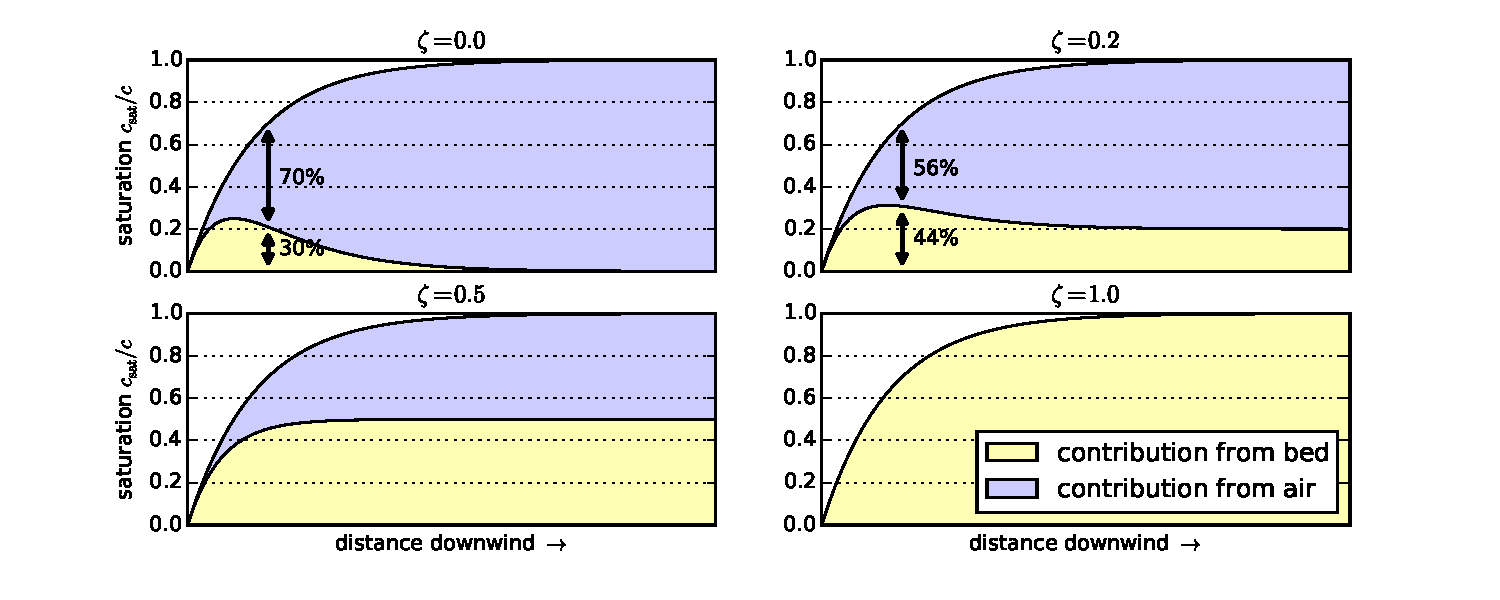
\includegraphics[width=\columnwidth]{../Figures/bed_interaction_parameter}
  \caption{Contributions of the grain size distribution in the bed and
    in the air to the weighting factors $\hat{w}_k$ for the
    equilibrium sediment concentration in Equation
    \ref{eq:erodep_multi} for different values of the bed interaction
    parameter.}
  \label{fig:bed_interaction_parameter}
\end{figure}

To allow for bed interaction in saturated situations in which no net
erosion can occur, the bed interaction parameter $\zeta$ is used (Figure
\ref{fig:bed_interaction_parameter}). The bed interaction parameter
can take values between 0.0 and 1.0 in which the weighting factors for
the equilibrium or saturated sediment concentration in an
(over)saturated situation are fully determined by the grain size
distribution in the bed or in the air respectively. A bed interaction
value of 0.2 represents the situation in which the grain size
distribution at the bed surface contributes 20\% to the weighting of
the saturated sediment concentration over the fractions. In the
example situation where the air is 70\% saturated such value for the
bed interaction parameter would lead to weighting factors that are
constituted for $70\% \cdot (100\% - 20\%) = 56\%$ based on the grain
size distribution in the air and for the other 44\% based on the grain
size distribution at the bed surface (Figure
\ref{fig:bed_interaction_parameter}, upper right panel).

The parameterization of the exchange of momentum between sediment
fractions is an aspect of saltation that is still poorly
understood. Therefore calibration of the bed interaction parameter
$\zeta$ is necessary. The model parameters in Equation
\ref{eq:equilibrium_transport} can be chosen in accordance with the
assumptions underlying multi-fraction sediment transport. $C$ should
be set to 1.5 as each individual sediment fraction is well-sorted,
$d_{\mathrm{n}}$ should be chosen equal to $D_{\mathrm{n}}$ as the
grain size dependency is implemented through
$u_{\mathrm{th}}$. $u_{\mathrm{th}}$ typically varies between 1 and 6
m/s for sand.

\subsection{Simulation of Sediment Sorting and Beach Armoring}

Since the equilibrium or saturated sediment concentration
$c_{\mathrm{sat},k}$ is weighted over multiple sediment fractions in
the extended advection model, also the instantaneous sediment
concentration $c_k$ is computed for each sediment fraction
individually. Consequently, grain size distributions may vary over the
model domain and in time. These variations are thereby not limited to
the horizontal, but may also vary over the vertical since fine
sediment may be deposited on top of coarse sediment or, reversely,
fines may be eroded from the bed surface leaving coarse sediment to
reside on top of the original mixed sediment. In order to allow the
model to simulate the processes of sediment sorting and beach armoring
the bed is discretized in horizontal grid cells and vertical bed
layers (2DV; Figure \ref{fig:bedcomposition}).

The discretization of the bed consists of a minimum of three vertical
bed layers with a constant thickness and an unlimited number of
horizontal grid cells. The top layer is the \textit{bed surface layer}
and is the only layer that interacts with the wind and hence
determines the spatiotemporal varying sediment availability and the
contribution of the grain size distribution in the bed to the weighting
of the saturated sediment concentration. One or more \textit{bed
  composition layers} are located underneath the bed surface layer and
form the upper part of the erodible bed. The bottom layer is the
\textit{base layer} and contains an infinite amount of erodible
sediment according to the initial grain size distribution. The base
layer cannot be eroded, but can supply sediment to the other layers.

\begin{figure}
  \centering
  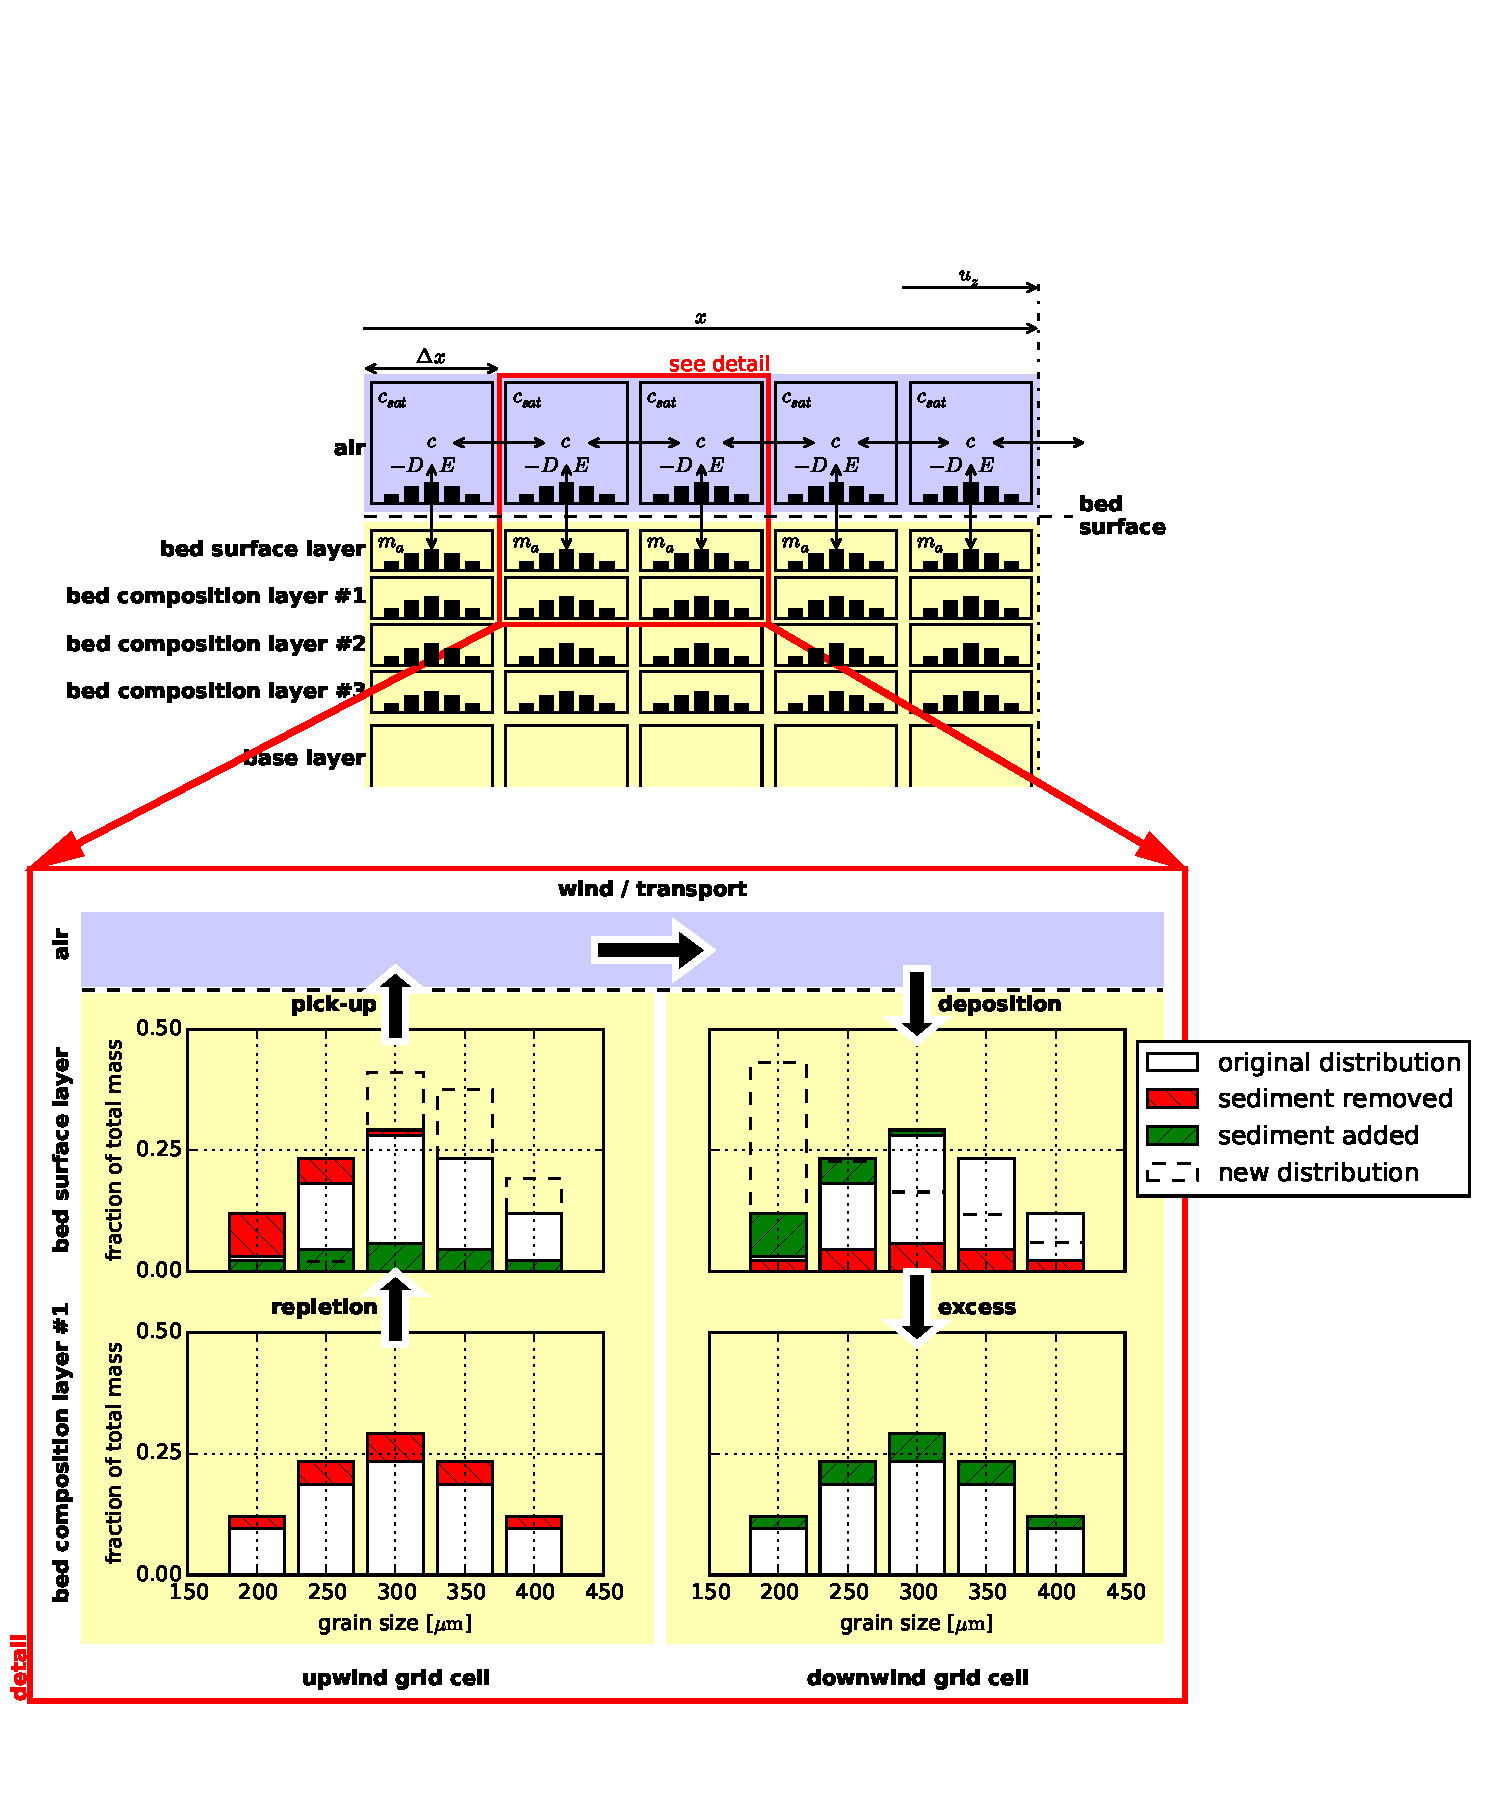
\includegraphics[width=\columnwidth]{../Figures/bedcomposition}
  \caption{Schematic of bed composition discretisation and advection
    scheme. Horizontal exchange of sediment may occur solely through
    the air that interacts with the \textit{bed surface layer}. The
    detail presents the simulation of sorting and beach armoring where
    the bed surface layer in the upwind grid cell becomes coarser due
    to non-uniform erosion over the sediment fractions, while the bed
    surface layer in the downwind grid cell becomes finer due to
    non-uniform deposition over the sediment fractions. Symbols refer
    to Equations \ref{eq:advection} and \ref{eq:erodep}.}
  \label{fig:bedcomposition}
\end{figure}

Each layer in each grid cell describes a grain size distribution over
a predefined number of sediment fractions (Figure
\ref{fig:bedcomposition}, detail). Sediment may enter or leave a grid
cell only through the bed surface layer. Since the velocity threshold
depends among others on the grain size, erosion from the bed surface
layer will not be uniform over all sediment fractions, but will tend
to erode fines more easily than coarse sediment (Figure
\ref{fig:bedcomposition}, detail, upper left panel). If sediment is
eroded from the bed surface layer, the layer is repleted by sediment
from the lower bed composition layers. The repleted sediment has a
different grain size distribution than the sediment eroded from the
bed surface layer. If more fines are removed from the bed surface
layer in a grid cell than repleted, the median grain size
increases. If erosion of fines continues the bed surface layer becomes
increasingly coarse. Deposition of fines or erosion of coarse material
may resume the erosion of fines from the bed.

In case of deposition the process is similar. Sediment is deposited in
the bed surface layer that then passes its excess sediment to the
lower bed layers (Figure \ref{fig:bedcomposition}, detail, upper right
panel). If more fines are deposited than passed to the lower bed
layers the bed surface layer becomes increasingly fine.

\subsection{Simulation of the Emergence of Non-erodible Roughness
  Elements} \label{sec:roughness}

Sediment sorting may lead to the emergence of non-erodible elements
from the bed. Non-erodible roughness elements may shelter the
erodible bed from wind erosion due to shear partitioning, resulting in
a reduced sediment availability \citep{Raupach1993}. Therefore
Equation \ref{eq:raupach} is implemented according to:

\begin{equation} \label{eq:raupach2}
u_{\mathrm{* th, R}} = u_{\mathrm{* th}} \cdot \sqrt{ \left( 1 - m \cdot \sum_{k=k_0}^{n_{\mathrm{k}}}{w_k^{\mathrm{bed}}} \right) \left( 1 + \frac{m \beta}{\sigma} \cdot \sum_{k=k_0}^{n_{\mathrm{k}}}{w_k^{\mathrm{bed}}} \right) }
\end{equation}

\noindent in which $\sigma$ is the ratio between the frontal area and
the basal area of the roughness elements and $\beta$ is the ratio
between the drag coefficients of the roughness elements and the bed
without roughness elements. $m$ is a factor to account for the
difference between the mean and maximum shear stress and is usually
chosen 1.0 in wind tunnel experiments and may be lowered to 0.5 for
field applications. The roughness density $\lambda$ in the original
equation of \citet[][Equation \ref{eq:raupach}]{Raupach1993} is
obtained from the mass fraction in the bed surface layer $w_k^{\mathrm{bed}}$
(Equation \ref{eq:massfraction}) according to:

\begin{equation}
\label{eq:roughness_density}
\lambda = \frac{\sum_{k=k_0}^{n_{\mathrm{k}}}{w_k^{\mathrm{bed}}}}{\sigma}
\end{equation}

\noindent in which $k_0$ is the index of the smallest non-erodible
sediment fraction in current conditions and $n_{\mathrm{k}}$ is the
total number of sediment fractions. It is assumed that the sediment
fractions are ordered by increasing size. Whether a fraction is
erodible depends on the sediment transport capacity.

\subsection{Simulation of the Hydraulic Mixing, Infiltration and
  Evaporation} \label{sec:marine_processes}

As sediment sorting due to aeolian processes can lead to armoring of a
beach surface, mixing of the beach surface or erosion of course
material may undo the effects of armoring. To ensure a proper balance
between processes that limit and enhance sediment availability in the
model both types of processes need to be sufficiently represented when
simulating spatiotemporal varying bed surface properties and sediment
availability.

A typical upwind boundary in coastal environments during onshore winds
is the water line. For aeolian sediment transport the water line is a
zero-transport boundary. In the presence of tides, the intertidal
beach is flooded periodically. Hydraulic processes like wave breaking
mix the bed surface layer of the intertidal beach, break the beach
armoring and thereby influence the availability of sediment. Moreover,
the hydraulic processes periodically wet the intertidal beach
temporally increasing the shear velocity threshold. Infiltration and
evaporation subsequently dry the beach.

In the model the mixing of sediment is simulated by averaging the
sediment distribution over the depth of disturbance
($\Delta z_{\mathrm{d}}$). The depth of disturbance is linearly
related to the breaker height \citep[e.g.][]{King1951, Williams1971,
  Masselink2007}. \citet{Masselink2007} proposes an empirical factor
$f_{\Delta z_{\mathrm{d}}}$ [-] that relates the depth of disturbance
directly to the local breaker height according to:

\begin{equation}
  \label{eq:dod}
  \Delta z_{\mathrm{d}} = f_{\Delta z_{\mathrm{d}}} \cdot \min \left ( H \quad ; \quad \gamma \cdot d \right )
\end{equation}

\noindent in which the offshore wave height $H$ [m] is taken as the
local wave height maximized by a maximum wave height over depth ratio
$\gamma$ [-]. $d$ [m] is the water depth that is provided to the model
through an input time series of water levels. Typical values for
$f_{\Delta z_{\mathrm{d}}}$ are 0.05 to 0.4 and 0.5 for $\gamma$.

The drying of the beach is simulated by simplified functions for
infiltration and evaporation. Infiltration is represented by an
exponential decay function that is governed by a drying time scale
$T_{\mathrm{dry}}$. Evaporation is simulated using an adapted version
of the Penman-Monteith equation \citep{Shuttleworth1993} that is
governed by meteorological time series of solar radiation, temperature
and humidity.

\section{Results} \label{sec:results}

The model is applied to a series of prototype cases to illustrate the
processes described by the model, two wind tunnel experiments to
illustrate the capabilities of the model to simulate spatiotemporal
variations in bed surface properties and sediment availability and a
sensitivity analysis.

\subsection{Prototype cases} \label{sec:prototype}

The four prototype cases P1 to P4 are intended to illustrate the
capabilities of the presented model to simulate processes of sediment
sorting \citep{VanDerWal2000, Arens2002} and beach armoring
\citep{VanDerWal1998}. The prototype cases are constructed using a 120
m schematized linear beach with a 1:20 slope, a wind velocity of 12 or
30 m/s, a drying time scale $T_{\mathrm{dry}}$ of 3 h, constant
evaporation and a simulation time of 30 days. The prototype cases are
initialized with lognormally distributed sediment with $d_{50} = 335$
$\mu \mathrm{m}$ ($\Phi-\mathrm{scale} = 1.6$, $\sigma_{\Phi} = 0.4$),
which is representative for nourished poorly sorted beaches along the
Dutch coast.  Parameterizations for shells and shell fragments in
Equation \ref{eq:raupach2} are based on experiments described by
\citet{McKennaNeuman2012} and chosen as $m = 0.5$, $\sigma = 4.2$ and
$\beta = 130$. The four scenarios described by the prototype cases
are:

\begin{description}
\item[P1] This scenario is used as reference for normalization and
  involves sand only and no tidal movement. The model is forced by a
  constant wind of 12 m/s. Sediment sorting occurs due to the presence
  of a wide range of sediment fractions. However, beach armoring does
  not occur due to the absence of shells, resulting in an almost
  constant sediment transport rate at the downwind end of the domain.
\item[P2] This scenario involves 5\% of shells and shell fragments
  ranging from 2 to 30 mm and no tidal movement. The model is forced
  by a constant wind of 12 m/s. The presence of shells means that beach
  armoring occurs that causes spatiotemporal variations in sediment
  availability and a decrease in sediment transport.
\item[P3] This scenario involves 5\% of shells and shell fragments and
  a sinusoidal tide with a 2 m tidal range and a tidal period of 12
  h. The tide periodically floods a 40 m intertidal beach area. The
  model is forced by a constant wind of 12 m/s. The tidal movement
  causes mixing of the bed surface layer in the intertidal beach area
  reducing the effects of beach armoring.
\item[P4] This scenario is equal to scenario P3, but the model is
  forced by a wind of 12 m/s that is increased twice to 30 m/s to
  simulate the effect of higher energy wind events that (partially)
  reset the composition of the bed surface layer and temporarily
  increase the sediment availability in the dry beach area.
\end{description}

\begin{figure}
  \centering
  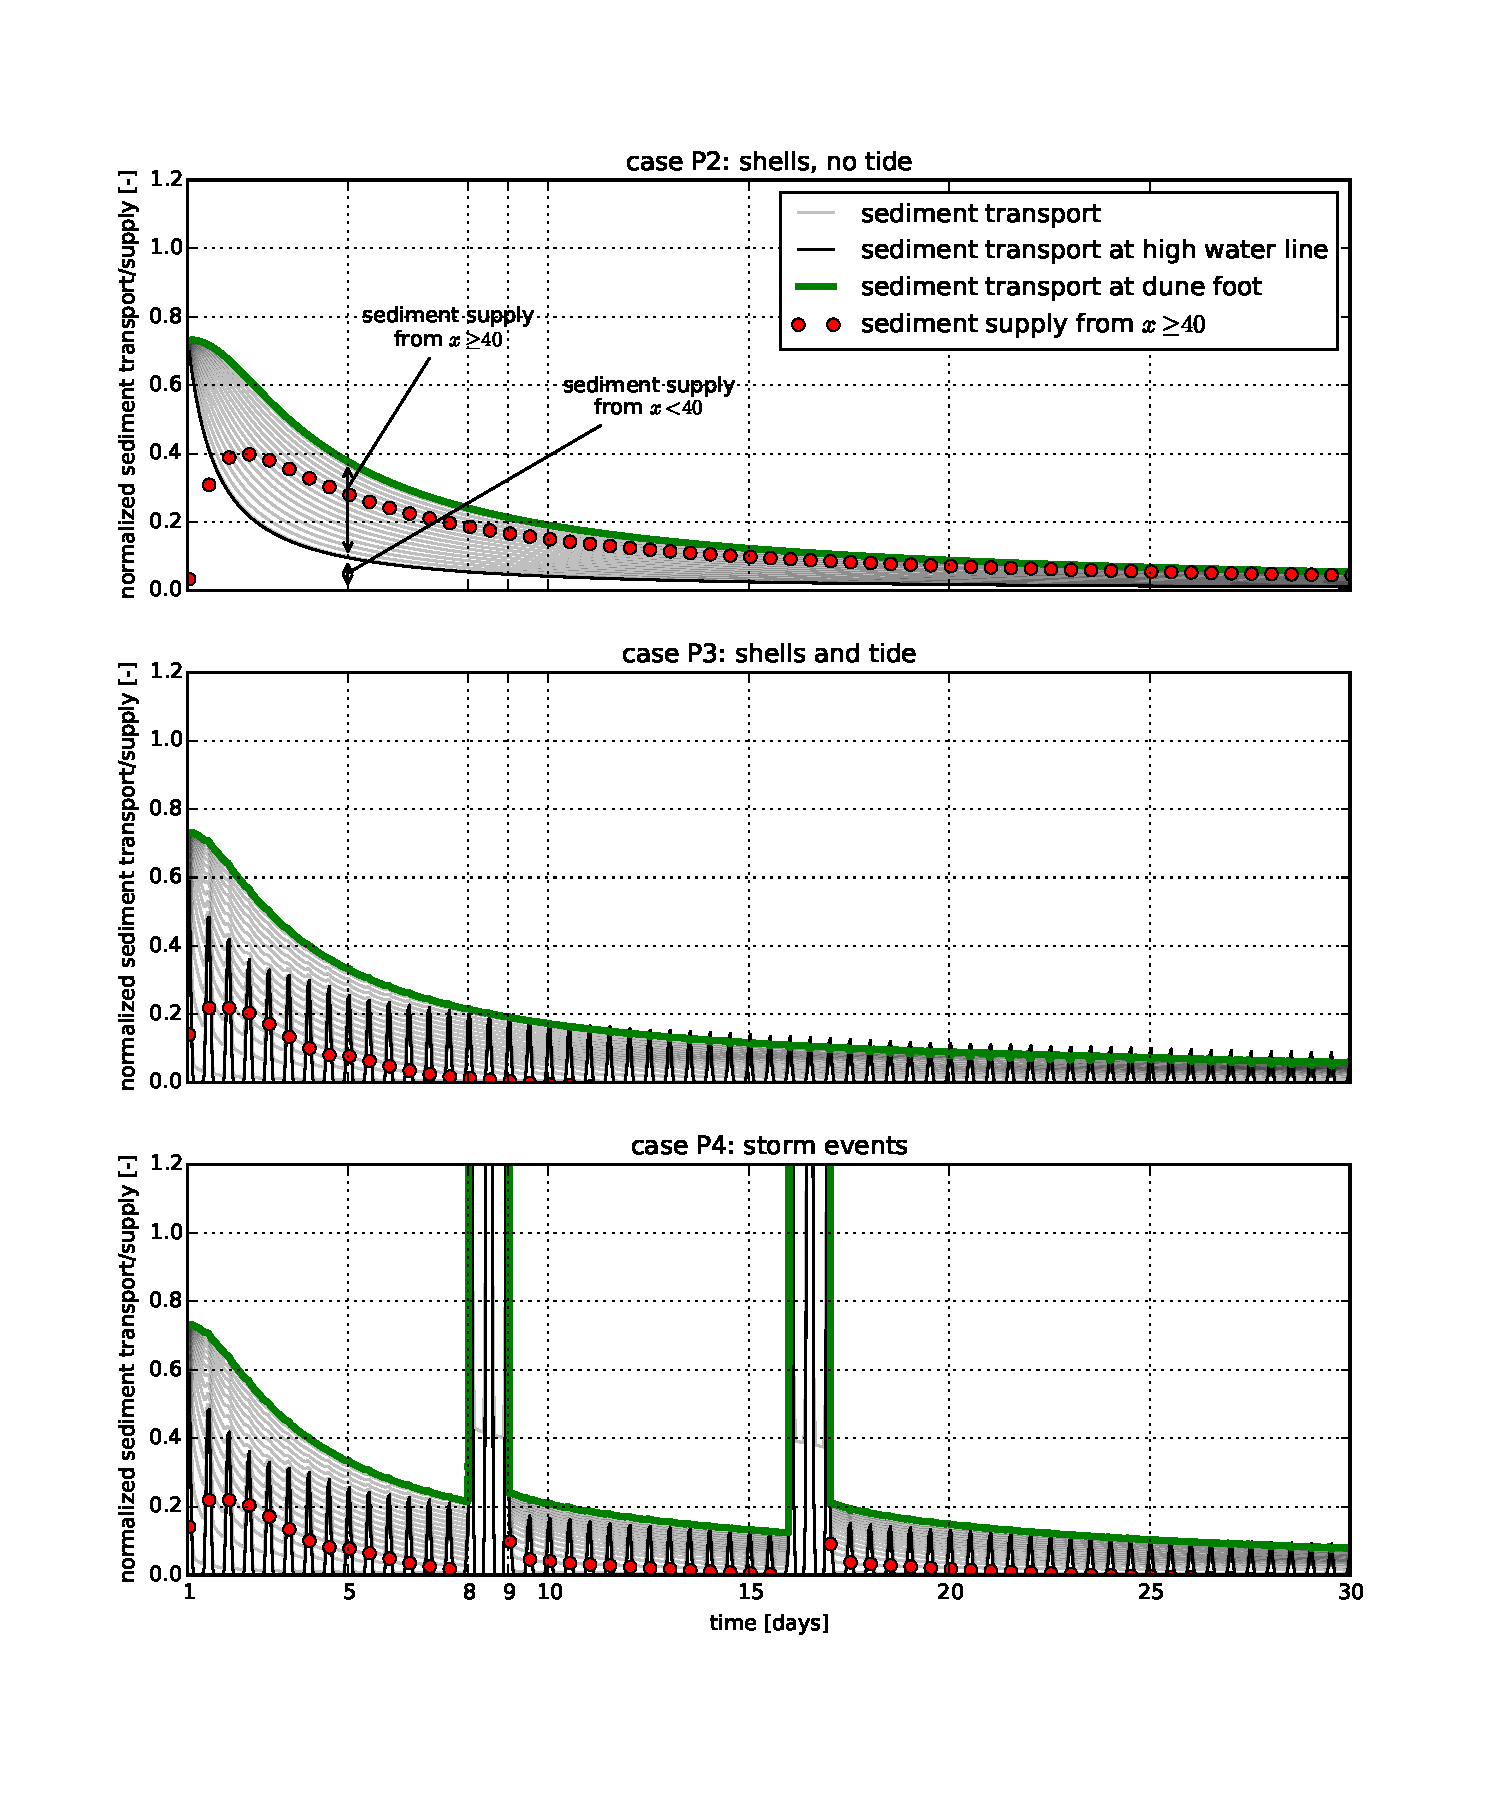
\includegraphics[width=\columnwidth]{../Figures/transport_rate_v2}
  \caption{Sediment transport in time and over the model domain for
    three scenarios with constant wind. Each line depicts a different
    location along the beach, starting from $x = 40$ m, which
    coincides with the high water line in cases P3 and P4, and ends at
    the dune foot. Results are normalized using the transport rate in
    case P1 with almost constant transport (not shown). The difference
    between the sediment transport at dune foot (green) and the
    sediment transport at $x = 40$ m is visualized by the red dots and
    represents the sediment supply from the dry beach. In cases P3 and
    P4 the sediment transport at the high water line periodically
    exceeds the sediment transport at the dune foot, indicating local
    deposition of sediments originating from the intertidal beach.}
  \label{fig:transport_rate}
\end{figure}

\begin{figure}
  \centering
  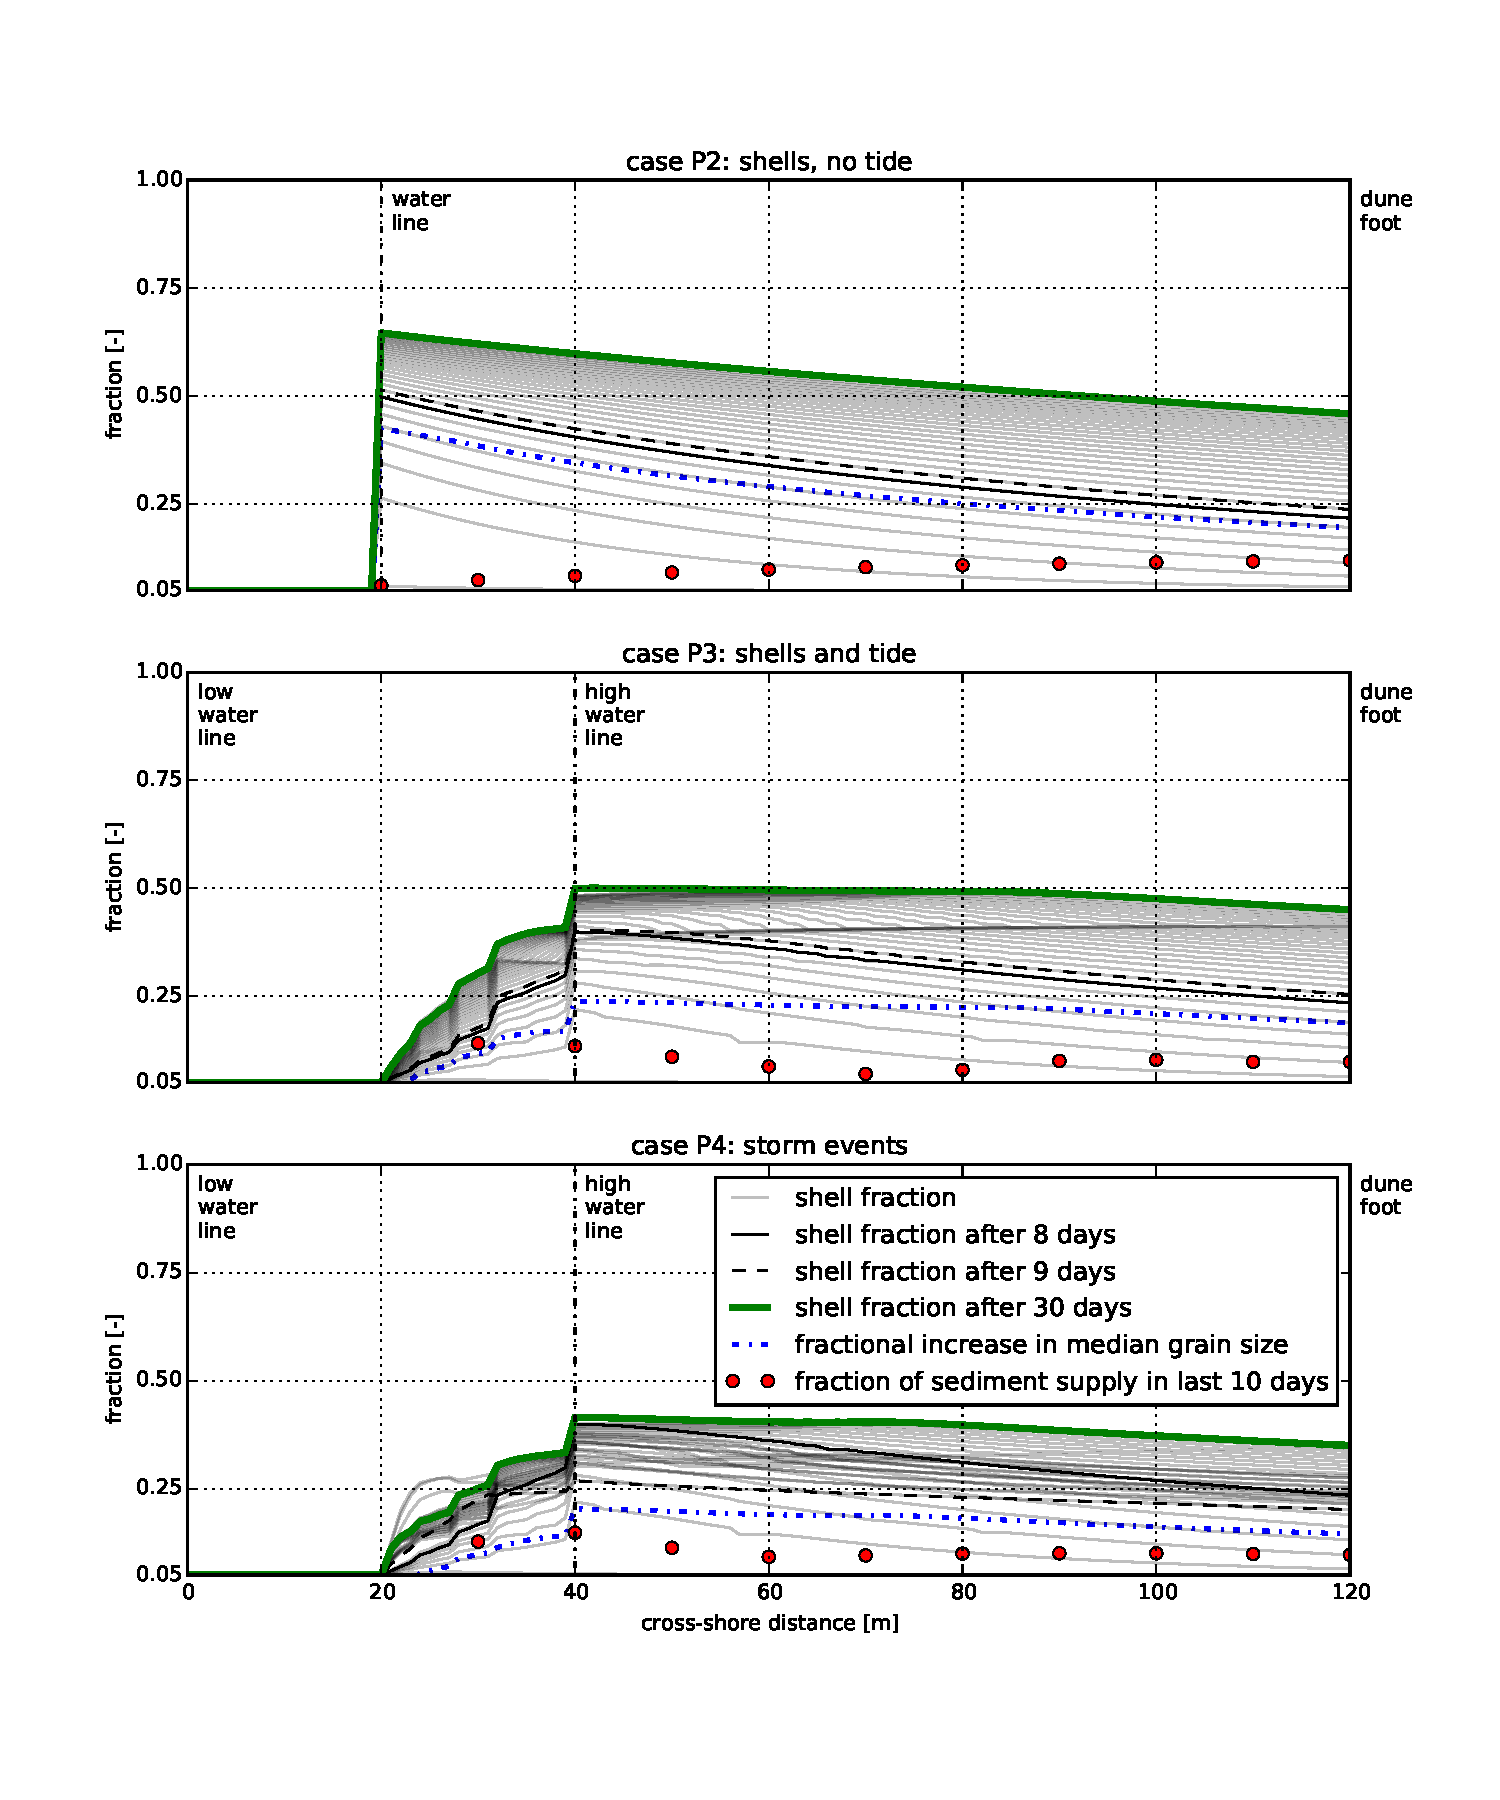
\includegraphics[width=\columnwidth]{../Figures/shell_fraction}
  \caption{Distribution of the shell fraction over the model domain
    and in time. Sediment supply is inversely related to the degree of
    beach armoring, indicated by the shell fraction. Median grain size
    increases with the increase in shell fraction indicating erosion
    of predominantly fines. High-energy wind events in case P4 even
    mobilize shell fractions resulting in a decrease in beach armoring
    and an increase in sediment availability.}
  \label{fig:shell_fraction}
\end{figure}

Figure \ref{fig:transport_rate} presents the simulated aeolian
sediment transport rates at the downwind end of the domain for cases
P2 to P4 over the course of 30 days of simulation time. The results
are normalized using the transport rate in case P1. The reference case
P1 shows an almost constant transport rate over the entire course of
the simulation. The presence of shells in case P2 results in a
reduction of sediment availability. As a result, the transport rates
in case P2 are lower compared to case P1. The transport rate decreases
as more shells emerge from the bed and a beach armor layer
develops. In case P2 there are no processes that break the armoring
and the transport rates asymptotically reach zero. The beach armor
layer develops in direction of the wind. Therefore, the relative
contribution of the downwind part of the beach ($x \geq 40$) to the
total sediment transport increases over time.

Case P3 includes tidal movement and hydraulic mixing. At the high
water line the sediment transport is zero during high tide and
maximized during low tide. Initially, transport is not saturated at
the high water line and entrainment of sediment continues over the dry
beach. As shells emerge from the bed, a beach armor layer develops
that reduces sediment availability. The reduction of sediment
availability progresses slower at the intertidal beach compared to the
dry beach due to hydraulic mixing. After 8 days the sediment transport
rates at the high water line start to exceed the sediment transport
rates at the dune foot during low water. Sediment that is eroded from
the intertidal beach during low water is partially trapped at the dry
beach due to differences in roughness. During subsequent high water,
when the sediment supply from the intertidal beach ceases, these
deposits are again entrained and blown downwind. The net erosion from
the dry beach ultimately approaches zero as armoring of the dry beach
progresses. At this point all sediment deposited downwind originates
directly from the intertidal beach. However, due to the spatial
differences in roughness, sediment is temporally deposited at the dry
beach and cause the sediment transport rates at the dune foot to be
only weakly correlated with the tidal movement.

Case P4 shows a pattern similar to case P3, but after 8 and 16 days a
relatively high-energy wind event passes for 24 hours. As a result,
the transport rate spikes, but an elevated transport rate is also
visible after the wind velocity drops.  During the high-energy wind
event even small shell fragments are mobilized. The beach armoring is
therefore (partially) removed and more sediment is available for
transportation afterwards. This leads to a prolonged peak in sediment
transport and an increase of the relative contribution of the dry
beach to the total sediment transport at the dune foot. After the
beach armoring is re-established over time the transport rates
approach the rates of case P3 again.

The differences in transport rate between the prototype cases are
directly related to sediment availability, since the wind is constant
in all cases but case P4. Figure \ref{fig:shell_fraction} shows the
fractions of shells and shell fragments in the bed surface layer for
case P2 to P4. The shell fraction increases over time in all
simulations. In case P2 the shell fraction peaks at the water line as
the beach armor layer develops in downwind direction. Consequently, at
the end of the simulation most sediment originates from the downwind
end of the beach where the beach armoring is least developed. In case
P3 and P4 hydraulic mixing causes the shell fraction in the intertidal
beach to remain low resulting in a different distribution of shells
compared to case P2 and hence a difference in sediment
availability. Consequently, at the end of the simulation most sediment
originates from the intertidal beach. In reality, the contribution of
the intertidal beach to the total sediment transport is likely to be
higher as more marine processes counteract the local development of a
beach armor layer than currently simulated, like marine deposits and
buoyancy of shells. In case P4 the drop in shell fraction from day 8
to day 9 is related to the first high-energy wind event. At the end of
the simulation, the fraction of sediment that originates from the
intertidal beach is relatively low compared to case P3. In all cases
also the median grain size in the bed surface layer increases,
indicating that predominantly fine sediment is eroded from the
bed. The unbalanced sediment transport over the fractions cause
sediment sorting in downwind direction.

%The prototype cases illustrate the potential importance of beach
%armoring for aeolian sediment transport estimates and the location of
%sediment source areas. Multi-fraction sediment transport drives the
%spatiotemporal variations in sediment availability due to the
%development of a beach armor layer. In addition, multi-fraction
%sediment transport simulates sorting of sediment in downwind
%direction.

The contribution to the instantaneous sediment transport of the
specific processes described by the model can be distinguished in the
prototype cases P1 to P4 because a constant wind velocity is
imposed. If a more realistic variable wind velocity time series is
used, the contributions of the specific processes are obscured by the
wind-related variance. To show that the simulation of spatiotemporal
bed surface properties and sediment are also important in variable
wind conditions, prototype cases P1 to P3 are repeated using an
synthetic variable wind time series (P1b to P3b). The time series is
generated using a Markov Chain Monte Carlo (MCMC) simulation following
a Weibull distribution with a mean wind velocity of 12 m/s.

Figure \ref{fig:variable_wind} shows the sediment transport rate in
case P3b normalized by the sediment transport rate in case P1b
depending on the hourly averaged wind velocity. To remove the
influence of the wind variability, the normalized sediment transport
time series obtained from the simulations are binned according to the
hourly averaged wind velocity in 0.5 m/s bins. The median transport
rate in each bin is subsequently determined to obtain a relation
between instantaneous normalized sediment transport and wind
velocity. The reduction is close to 100\% up to wind velocities of 5
m/s and subsequently decreases according to an exponential
function. The median reduction for 12 m/s wind velocity is 74\%, which
is less than the maximum reduction of 95.0\% with a constant 12 m/s
wind velocity in case P3. The reduction tends to increase during the
simulation as beach armoring progresses.

\begin{figure}
  \centering
  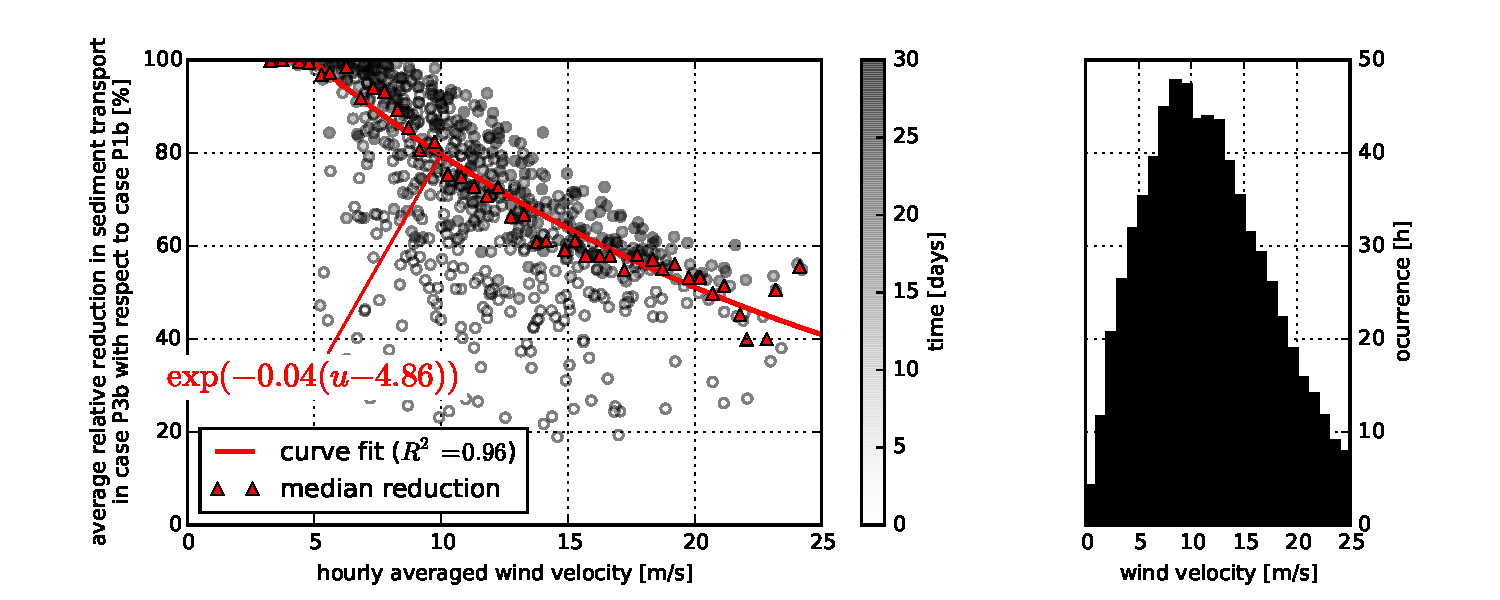
\includegraphics[width=\columnwidth]{../Figures/variable_wind_py}
  \caption{Average reduction in sediment transport in prototype case
    P3b compared to case P1b depending on the hourly averaged wind
    velocity (left panel). The results are obtained using an synthetic
    variable wind time series following a Weibull distribution with a
    mean wind velocity of 12 m/s (right panel). The sediment transport
    reduction (scatter) is binned according to the wind velocity using
    0.5 m/s bins. The median reduction per bin (triangles) is used to
    fit an exponential curve (line). The reduction tends to increase
    during the simulation (scatter colors).}
  \label{fig:variable_wind}
\end{figure}

\subsection{Wind tunnel experiments} \label{sec:windtunnel}

To illustrate the applicability of the model approach, two unrelated
wind tunnel experiments obtained from literature are simulated that
involve either temporal \citep{Nickling1995} or spatial
\citep{Dong2004b} variations in bed surface properties as discussed in
section \ref{sec:challenges}.

\citet{Nickling1995} describe an experiment in a wind tunnel with a
4.5 m working section in which a grid of 18 mm marbles was buried in
sandy material with $d_{50} = 270$ $\mu \mathrm{m}$.  During the
experiment with constant wind of 8 m/s, measured at 25 cm above the
bed, the sand is winnowed from in between the marbles resulting in the
emergence of the marbles over time. The emergence of the marbles cause
the bed to become armored. The effect of armoring of a marble extends
beyond the marble dimensions due to shadowing effects in the lee of
the marble described by Equation \ref{eq:raupach2}. All parameter
values, including $z'$, are obtained from \citet{Nickling1995} and
hence no further calibration of parameters is performed for this
simulation.

Figure \ref{fig:nickling1995} shows the modeled normalized sediment
transport rate in comparison with the measurements described in
\citet{Nickling1995}. Where the measurements start with a relatively
constant transport and even a slight increase in transport, the model
predicts an immediate decrease in transport. The marbles are modeled
as a large sediment fraction for which its presence in a bed
composition layer is described by a mass fraction rather than a
location. Therefore, it is possible to define the marble density, but
not the exact marble locations. Consequently, from the start of the
simulation marbles start to emerge from the bed resulting in an
immediate decrease in sediment transport. In contrast, in the wind
tunnel the marbles are covered with a thin layer of sand that was
removed first before the marbles start to emerge. The initial
emergence of the marbles coincided with a slight increase in sediment
transport. \citet{Nickling1995} attributes this rise to a pronounced
change in boundary conditions and turbulence. Since these small scale
variations in the wind shear are not represented in the model the rise
in transport is not visible in the model results. However, the
decrease in sediment transport due to the emergence of the marbles for
the three different grid spacings described in \citet{Nickling1995},
is qualitatively represented by the model.

\citet{Dong2004b} describe an experiment in a wind tunnel with a 21 m
working section in which a patch of gravel with diameter 10 -- 40 mm
was positioned downwind of a sandy bed with $d_{50} = 180$
$\mu \mathrm{m}$. The length of the gravel patch was varied between
the experiments from 0.5 -- 12 m and the wind velocity from 8 -- 22
m/s, measured at 60 cm above the bed. The free-flow wind velocities
are converted to shear velocities assuming $z'$ = 6 mm. The gravel
patch traps saltating grains. In the model the entrapment of grains is
simulated as an exchange of momentum between the sandy fractions and
the immobile gravel fraction. This exchange is governed by the bed
interaction parameter, which is calibrated for this simulation and
found to be 0.05.

Figure \ref{fig:dong2004} shows the modeled sediment transport rate in
comparison with the measurements described in \citet{Dong2004b}. The
increase in sediment transport with increasing wind velocity is well
represented by the model given the uniform RMSE among the different
wind velocities. The decrease in sediment transport rate with
increasing gravel patch length is represented by the model with a
relative RMSE of less than 10\% for all except the lowest and highest
wind velocities. Significant surpassing of sediment over the sediment
trap during the measurements with 22 m/s wind velocity is reported by
\citet{Dong2004b}, which explains the consistent overprediction of the
sediment fluxes by the model. The discrepancy between the model and
the measurements for the 8 and 10 m/s wind velocities is less
consistent and is expected to be a result of a low signal-to-noise
ratio related to the small sediment fluxes. Also for short gravel
patch lengths the model deviates from the measurements. The relatively
high variability over the 0.5 to 2 m gravel patch lengths is
attributed to a change in transport characteristics \citep{Dong2004b}
due to fully elastic collisions between the sand grains and the
gravel. A bed interaction parameter that is not constant is needed to
capture this behavior in the model.

\begin{figure}
  \centering
  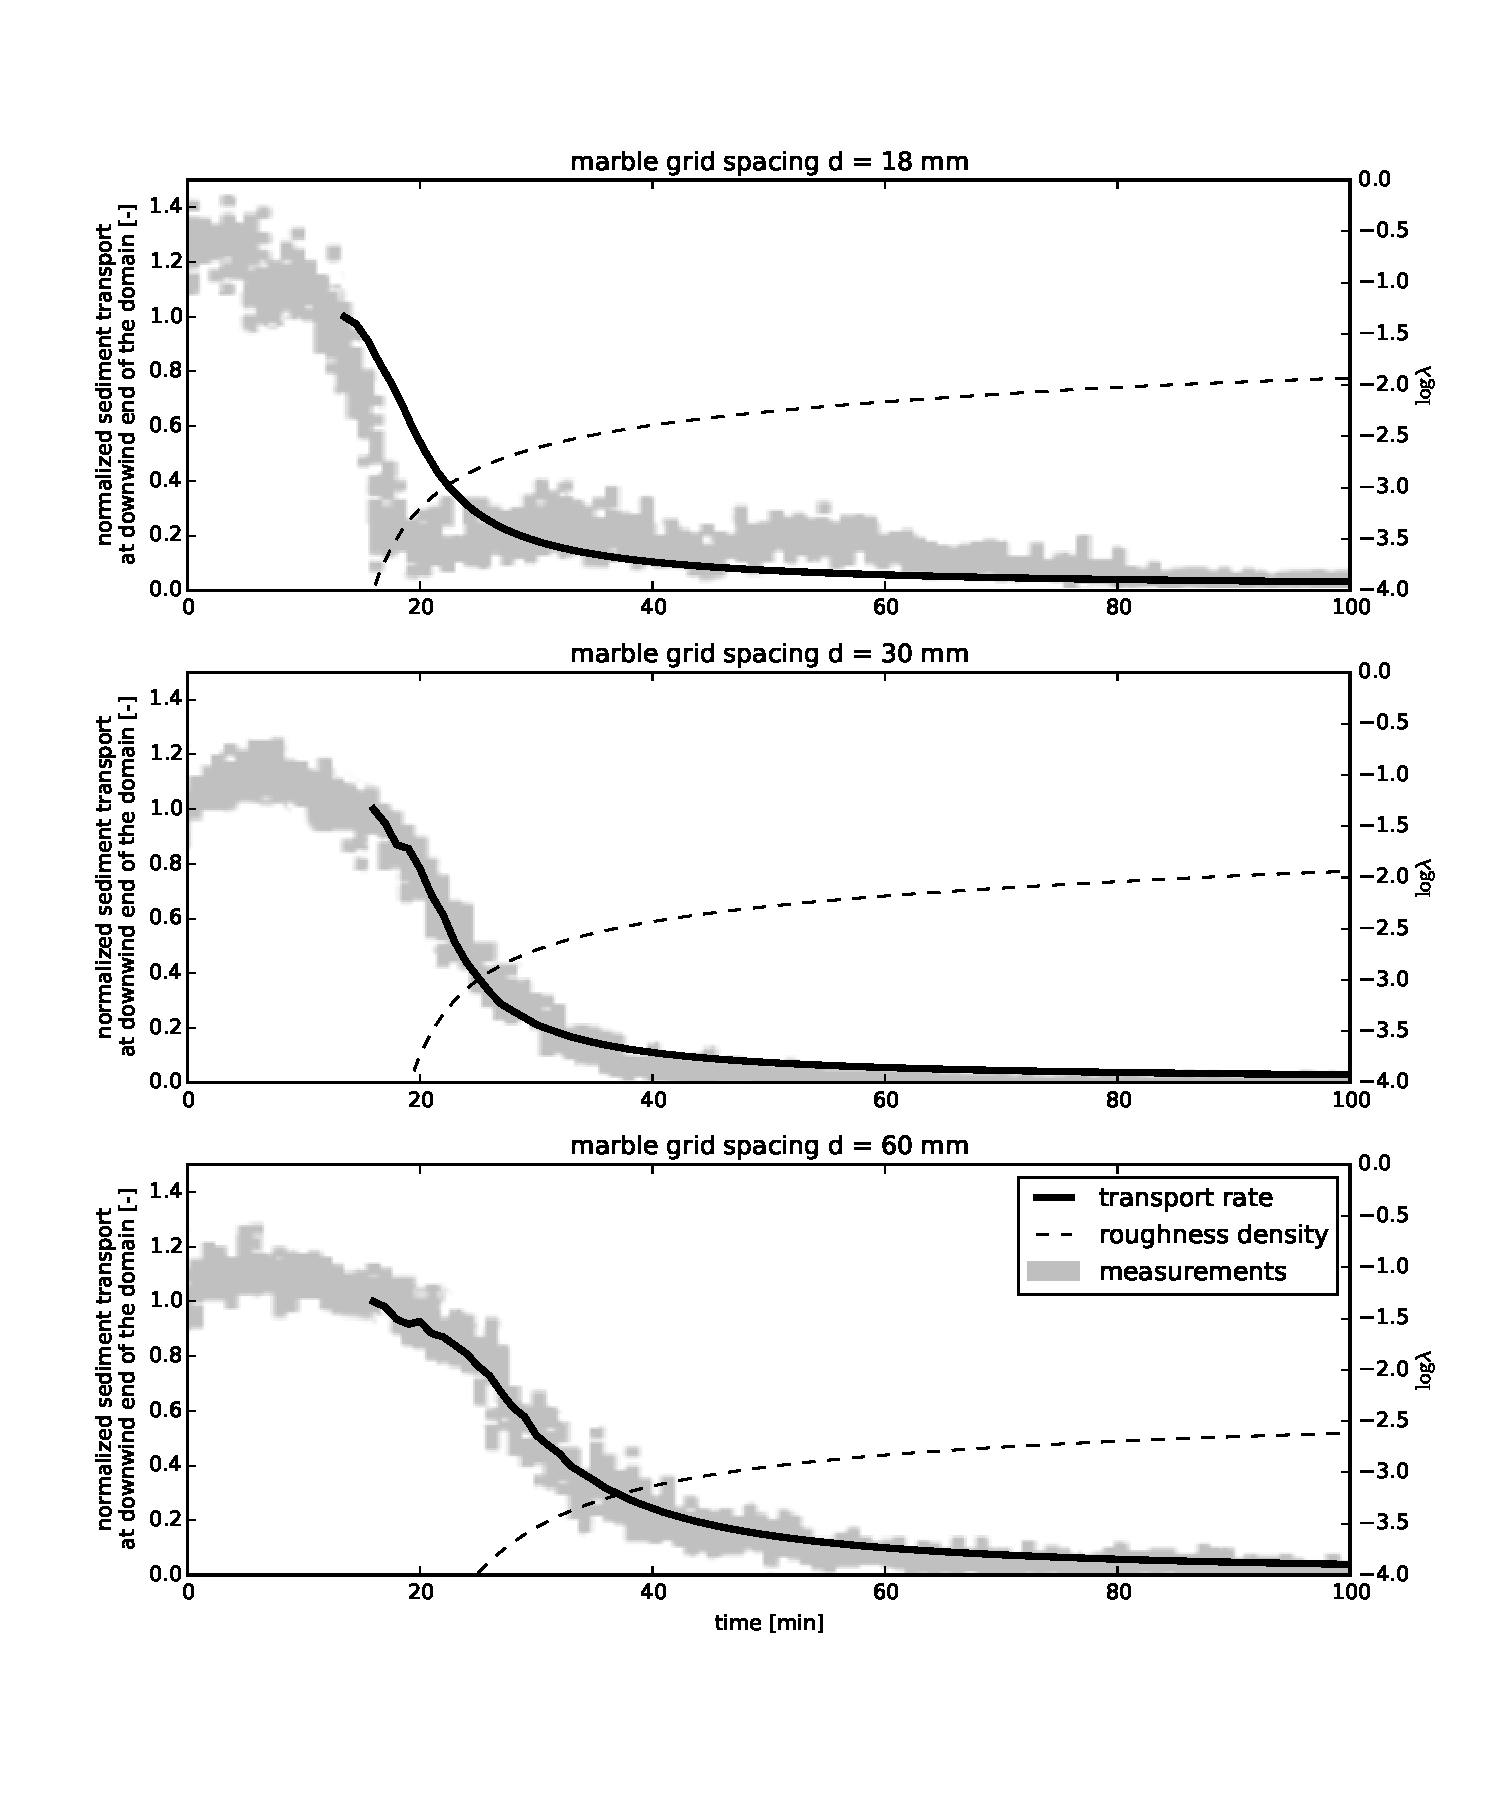
\includegraphics[width=\columnwidth]{../Figures/nickling1995_py}
  \caption{Comparison between modeled and measured normalized sediment
    transport rates from wind tunnel experiments described in
    \citet{Nickling1995}. The dashed line depicts the emergence of
    marbles in terms of increasing roughness density. The
    visualization of the measurement results is copied from Figure 4
    in the original publication without digitization.}
  \label{fig:nickling1995}
\end{figure}

\begin{figure}
  \centering
  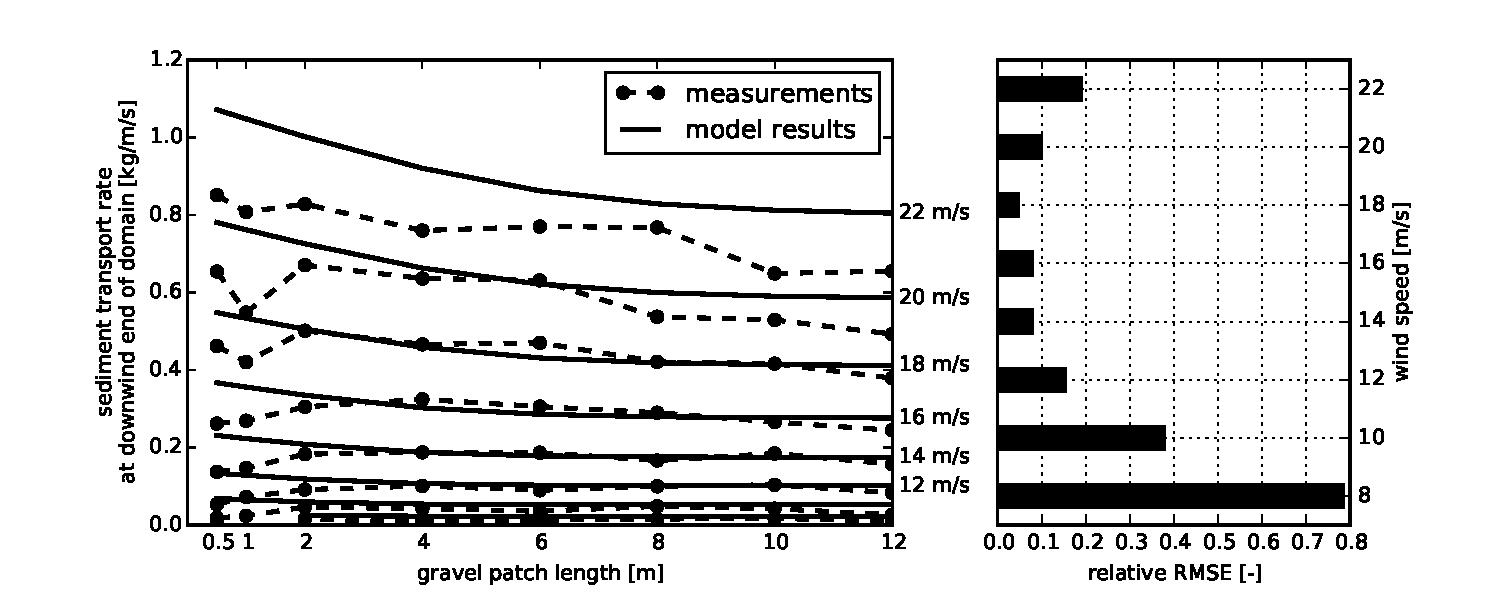
\includegraphics[width=\columnwidth]{../Figures/dong2004_py}
  \caption{Comparison between model results and measurements from wind
    tunnel experiments described in \citet{Dong2004b} (left panel) and
    RMS errors relative to the mean measured transport rate (right
    panel). The measured transport rates with a wind velocity of 22
    m/s are underestimated due to surpassing of sediment over the
    sediment trap \citep{Dong2004b}.}
  \label{fig:dong2004}
\end{figure}

\subsection{Sensitivity}

The sensitivity of the model to four newly introduced parameters and
the wind velocity is determined to obtain insight in the importance of
these parameters to the model results. The newly introduced parameters
are the bed interaction parameter, depth of disturbance factor, the
drying time scale and the grain size distribution standard
deviation. Case P3 as presented in section \ref{sec:prototype} is used
as starting point for the sensitivity analysis. Figure
\ref{fig:sensitivity} shows the change in normalized total sediment
transport given variations of each of the four model parameters and
the wind velocity.

\begin{figure}
  \centering
  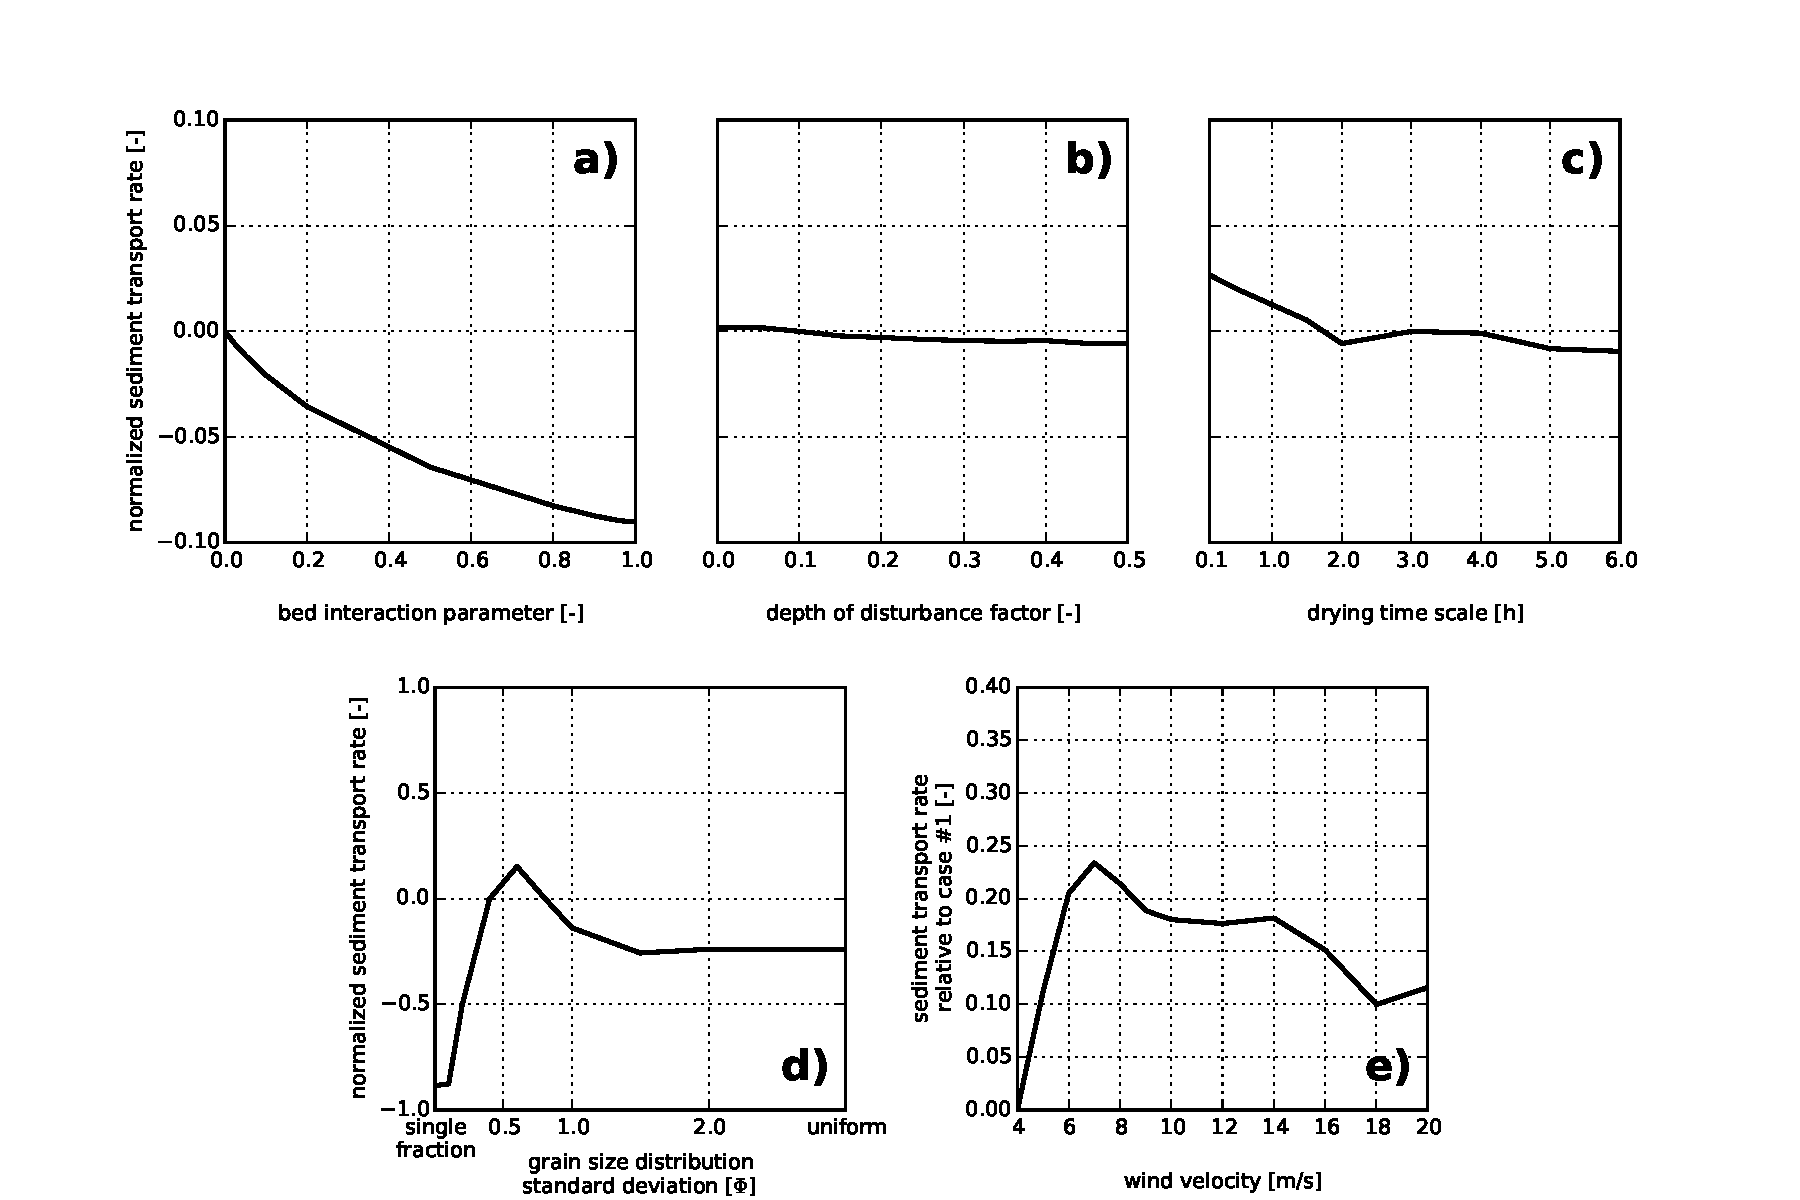
\includegraphics[width=\columnwidth]{../Figures/sensitivity_py}
  \caption{Sensitivity of the total normalized sediment transport with
    respect to case P3 for four newly introduced parameters and the
    wind velocity. The sensitivity of the wind velocity is expressed
    with respect to the transport rate in case P1.}
  \label{fig:sensitivity}
\end{figure}

The bed interaction parameter, the depth of disturbance factor and the
drying time scale affect the source area of aeolian sediment (Figure
\ref{fig:sensitivity}a, b and c). In absence of bed interaction all
sediment entrained in the intertidal beach area is being transported
to the downwind end of the domain unhindered. In contrast, in the
presence of bed interaction sediment from the intertidal beach area
may be trapped in the beach armor layer that is being developed in the
dry beach area during the simulation. Consequently, the total sediment
transport reduces with increasing bed interaction. The bed interaction
parameter parameterizes the exchange between sediment fractions, which
is an aspect of saltation that is still poorly understood.  In
particular situations with a large spatial variability in bed surface
properties the bed interaction parameter is expected to show a more
significant sensitivity \citep[e.g.][]{Dong2004b}. Therefore
calibration of the bed interaction parameter is necessary in such
situations.

The depth of disturbance factor shows no significant sensitivity as
aeolian sediment supply from the intertidal beach is concentrated
close to the water line where wave heights are negligible. Lower parts
of the intertidal beach are continuously too moist for sediment to be
entrained. The sensitivity to the depth of disturbance factor
increases with decreasing drying time scale, but typically only for
values smaller than 0.5 m.  The sensitivity to the drying time scale
shows that for time scales larger than several hours the intertidal
beach is continuously too moist for sediment to be entrained. For
small drying time scales the intertidal beach supplies aeolian
sediment that contains relatively many fines, resulting in a slight
increase in total sediment transport.

% The depth of disturbance factor and the drying time scale show a
% significant sensitivity (Figure \ref{fig:sensitivity}b and c). These
% parameters govern the sediment availability in the intertidal beach
% zone, which is ultimately the prime sediment source in case P3. In
% general, the large sensitivity to these parameters is expected in
% simulations where both beach armoring and tides play a role. Both
% parameters are related to peripheral processes in the presented
% model that are currently implemented using simplified
% formulations. Given the large sensitivity it seems advisable to
% further validate and possibly improve the implementation of these
% processes, which is considered outside the scope of this paper.
%
% For extreme values of both the depth of disturbance factor and the
% infiltration time scale the sensitivity reduces significantly. The
% sensitivity reduces for large depths
% ($f_{\Delta z_{\mathrm{d}}} > 0.5$) as the amount of fines becomes
% larger than the cumulative sediment transport capacity during the
% simulation.  The infiltration time scale shows two extreme
% situations in which the soil either does not dry out within a tidal
% cycle ($T_{dry} > 20$ h) or dries out instantly ($T_{dry} < 1$ h).

From the sensitivity of the grain size distribution width, represented
by the grain size distribution standard deviation and strictly
speaking not a model parameter, it can be concluded that the
introduction of multiple sediment fractions has a significant impact
on the sediment transport rate (Figure \ref{fig:sensitivity}d).
However, for poorly sorted sediments the sensitivity of the model to
the distribution width is limited. Beyond a standard deviation of
$\sigma_{\Phi} = 1.5$ the development of the sediment rate is similar
to the transport rate with a uniform distribution.

% The lowest sensitivity of the model is found for the bed interaction
% parameter (Figure \ref{fig:sensitivity}a). The bed interaction
% parameter parameterizes the exchange between sediment fractions,
% which is an aspect of saltation that is still poorly
% understood. Therefore calibration of the bed interaction parameter
% is necessary. A low sensitivity is beneficial as it reduces the
% importance of calibration. However, in particular situations with a
% large spatial variability in bed surface properties the bed
% interaction parameter is expected to show a more significant
% sensitivity \citep[e.g.][]{Dong2004b}.

The rate of armoring depends on the presence of non-erodible sediment
fractions. Whether a sediment fraction is erodible depends on the wind
transport capacity. Therefore the rate of armoring and consequently
the instantaneous sediment availability depends on the wind
velocity. Figure \ref{fig:sensitivity}e depicts the sediment transport
rate in case P3 with respect to the almost constant transport rate in
case P1 for different wind velocities. For low wind velocities all
shell fractions can contribute to the establishment of a beach armor
layer, but the beach armor layer develops slowly as the winnowing of
fines is dependent on the entrainment rate. For high wind velocities
even shell fragments may be mobilized, but the beach armor layer
consisting of larger shells is developed quickly. Consequently, the
reduction of sediment transport is present over all wind velocities
and 83\% on average.

% For low wind velocities all shell fractions can contribute to the
% establishment of a beach armor layer and consequently the sediment
% transport in case P3 is negligible compared to the transport rate in
% case P1. For high wind velocities, even shell fractions are
% mobilized and the importance of the beach armor layer
% reduces. Consequently, the sediment transport rates in case P3
% approach those of case P1 for high wind velocities.

\section{Discussion}

Process-based simulation of bed surface properties and sediment supply
provides an alternative for complex spatiotemporal
parameterizations. Nevertheless, process-based simulation itself
requires parameterization, calibration and validation. These
parameterizations are generally less complex as they describe static
properties rather than spatiotemporal varying processes.

\subsection{Parameterization}

Compared to existing models for availability-limited aeolian sediment
transport the need for complex parameterization has been reduced in
the presented model. The adoption of the advection model of
\citet{deVries2014a} makes parameterization of spatiotemporal
variations in the shear velocity threshold, like attempted by
\citet{Nickling1995}, \citet{Dong2004b} and others, unnecessary. In
addition, process-based simulation of bed surface properties makes
parameterization of the inherently time-varying sediment availability
$m_{\mathrm{a}}$ unnecessary. Existing parameterizations for the shear
velocity threshold under influence of moisture, vegetation, sediment
sorting and other bed surface properties are still valid for the
instantaneous shear velocity threshold.
% The proposed model provides a natural distinction between the fluid
% and impact threshold as these are related to the sediment
% availability and transport capacity that are both explicitly
% defined.

Despite the efforts to minimize complex parameterizations that are
difficult to generalize, the model also introduces new
parameterizations that are specifically related to the process-based
simulation of sediment availability, i.e. the bed interaction
parameter, depth of disturbance and soil drying time scale. The depth
of disturbance and soil drying time scale could easily be replaced by
process-based simulation as there is thorough knowledge on near-shore
morphodynamics and beach hydrology. Moreover, the presented model
framework allows for spatiotemporal variations of parameters that are
known not to be constant (e.g. $z'$). However, these considerations
are outside the scope of this paper and will be part of future
research.

\subsection{Calibration}

The calibration of the parameters involved in process-based simulation
of sediment availability is a relatively new field of research. In
this paper a pragmatic approach to calibration of these parameters is
adopted, but there are various opportunities for improvement. For
example, the depth of disturbance is used to approximate the mixing of
the intertidal beach surface by waves. \citet{Masselink2007} shows how
the depth of disturbance can be determined based on a linear relation
with the local wave height. The mixing of the intertidal beach surface
is particularly important as it breaks beach armoring. The depth of
disturbance does not provide any information about how the bed is
disturbed, just over which depth. Moreover, aspects like marine
deposits and shell buoyancy also affect the sediment availability in
the intertidal beach area. \citet{Gallagher2011} presented detailed
measurements of spatiotemporal variations in the bed surface grain
size at Truc Vert, France. The intertidal beach appears to be
consistently finer than the upper beach. The measurements are obtained
using macrophotography \citep{Buscombe2010} ensuring that the
measurements solely involve the beach surface. These type of
measurements may provide a much more detailed calibration of the
hydraulic mixing simulated in the model, although it might be
questioned if such detailed hydraulic calibration is still within the
scope of an aeolian sediment transport model. Alternatively, the
calibration of the hydraulic mixing could be left to dedicated
near-shore models \citep[e.g. XBeach;][]{Roelvink2009,Reniers2013} and
online model coupling could be used to incorporate detailed near-shore
hydro- and morphodynamics in the proposed aeolian modeling framework.

Similarly, an exponential decay function with a constant drying
time scale is currently used to approximate the influence of the
hydrological process of infiltration. The exponential decay is a
simplified approach that was adopted after it appeared to be a
reasonable approximation of numerical model results obtained with the
HYDRUS model \citep{Simunek1998} that simulates the soil moisture
contents in the unsaturated zone following
\citet{Genuchten1978}. Detailed measurements for calibration of the
instantaneous soil moisture can be obtained relatively easy using
either in-situ or remote infra-red or microwave measurements
\citep[e.g.][]{Edwards2013, Hoonhout2014}. Again, it might be
questioned if the amount of detail involved in using these kind of
data for estimates of the bed surface moisture is still within the
scope of an aeolian sediment transport model.

In contrast to the depth of disturbance and the drying rate, the bed
interaction parameter has little relation with existing literature. In
essence, the bed interaction parameter describes the exchange of
momentum between grain size fractions along the fetch
distance. Specifically it describes whether impacting grains eject
other grains from the bed or that they are rebounded due to fully
elastic collisions with large, non-erodible elements. A low value for
the bed interaction parameter would indicate a large number of
rebounding grains, while a high value would indicate a low number of
rebounding grains. Typically, the number of rebounded grains increases
with an increasing number of non-erodible, large elements in the
bed. Consequently, the bed interaction parameter is not uniform over
the fractions. Moreover, due to beach armoring the bed interaction is
neither constant over time nor in space. In this paper the bed
interaction parameter is pragmatically assumed to be uniform and
constant since no basis for differentiation of the parameter is
currently available. Thorough calibration of the bed interaction
parameter would require detailed, spatiotemporal measurements of grain
size distributions in the bed and the saltation cascade. It would
require a series of sediment traps along the fetch that are regularly
emptied and sieved as to determine the change of the grain size
distribution in the saltation cascade in space and over
time. Concurrently the grain size distribution at the bed surface over
the entire fetch needs to be monitored without disturbing the bed
significantly. In a laboratory environment the change in grain size
distribution could be monitored using sediment that is colored per
fraction. Visual observation of the change in coloring then provides
insight in the change in grain size distribution. However, the
experiment should be performed at such scale that the trapping of
sediment by upwind traps does not significantly influence the
saltation cascade downwind over the period that the armor layer
develops.

\subsection{Validation}

Validation of the proposed model is ongoing. Initially, validation
will be focused on gross sediment transport rates in
availability-limited systems. Few holistic measurements are available
that monitor both the spatiotemporal variations in the sediment
transport rate and the availability-limiting factors like moisture
content and beach armoring concurrently
\citep[e.g.][]{DelgadoFernandez2012, Hoonhout2013}. Sites with
detailed and frequent topographic measurements and hydrodynamic
boundary conditions available can be found worldwide. These sites
would be a good starting point for assessing the performance of the
model compared to existing models. Using simplified, but generic
descriptions of the hydraulic mixing and drying rate the model should
already provide time series of aeolian sediment transport that adhere
much better to the true nature of aeolian sediment transport events
than existing models. \citet{DelgadoFernandez2011} and
\citet{deVries2014b} already indicated that the true nature of these
events is not solely related to wind velocity and direction, but also
to surges, seasons, spring/neap cycles, rain showers and other events
that influence sediment availability. The variations in aeolian
sediment transport due to these event-driven changes in sediment
availability are not well captured by models that rely solely on the
wind transport capacity. The model has added value if it improves the
prediction of transport rates under such circumstances.

%\subsection{Model coupling}
%
%Apart from calibration and validation of the proposed model it is
%worth examining how this model and the related knowledge on
%availability-limited systems can be fitted in the broader
%understanding of coastal dynamics. As illustrated in this paper,
%aeolian sediment transport cannot be seen independently of near-shore
%hydrodynamics and related sediment transport, hydrology and probably
%also meteorology. Combining all these processes in a single sediment
%transport model would be cumbersome. Most prominently it would involve
%the combination of processes at time scales from seconds to
%years. Mathematically this would be challenging in terms of optimal
%numerical schemes and related time steps. Practically, as excellent
%models that simulate these processes already exist, it would require
%close and permanent collaboration between disciplines which might not
%be feasible on the long term.
%
%Instead, existing models could be seen as building blocks in a larger
%modeling framework for coastal sediment transport. This philosophy is
%the basis of online model coupling techniques, like the Earth System
%Modeling Framework \citep[ESMF;][]{Hill2004} and the Basic Model
%Interface \citep[BMI;][]{Peckham2013}. Online model coupling allows
%model cores to communicate with each other during the simulation. A
%near-shore hydrodynamic model like XBeach \citep{Roelvink2009} can
%therefore supply detailed descriptions of the water level, wave height
%and near-shore morphodynamics like onshore bar migration
%\citep{Cohn2015} to an aeolian sediment transport model. A
%hydrological model like HYDRUS \citep{Simunek1998} might be used to
%estimate instantaneous bed surface moisture contents. Even the wind
%field might be borrowed from a model like the highly efficient Coastal
%Dune Model \citep[CDM;][]{Duran2013}. In conclusion, online model
%coupling provides an elegant alternative to the few simplified
%implementations currently used in the proposed model.

\section{Conclusions}

The \textsc{AeoLiS} model presented in this paper is the first aeolian
sediment transport model that simulates spatiotemporal variations in
bed surface properties and sediment availability. Simulation of
sediment availability is necessary as sediment availability cannot be
determined a-priori due to its recurrence relation with sediment
transport. The presented model approach is a generalization of
existing modeling concepts for aeolian sediment transport that include
the influence of bed surface properties and limitations in sediment
availability, like the shear velocity threshold and critical fetch,
and is compatible with these concepts. The model uses an advection
scheme following \citet{deVries2014a} and a bed composition module
that discretizes the bed in horizontal grid cells and vertical bed
layers to account for spatial variations in bed surface
properties. Temporal variations in sediment availability are not
parameterized, but simulated using the bed composition module. The
simulation of sediment availability reduces the need for complex
spatiotemporal parameterizations and consequently calibration. In this
paper the influence of sediment sorting and beach armoring and the
reversed process of hydraulic mixing on aeolian sediment transport are
illustrated using four prototype cases. The model can reproduce
patterns in aeolian sediment availability and transport as observed in
wind tunnel experiments that involve spatiotemporal variations in bed
surface properties \citep{Nickling1995, Dong2004b}. Further, the model
provides a generic framework to incorporate additional spatiotemporal
varying processes that either influence sediment availability or the
wind transport capacity with a minimum of parameterization. The
framework allows relatively straightforward implementation of the
effects of infiltration, evaporation, vegetation, buildings, and
morphological feedback with the wind.
%Also, the model allows for
%online coupling with other models that accurately describe related
%physics that are currently parameterized like hydrodynamics, hydrology
%and meteorology.

\vspace{.5cm}

\noindent From this paper the following conclusions can be drawn:

\begin{enumerate}
\item A model for aeolian sediment transport was presented that
  simulates the processes of sediment sorting and beach armoring, the
  reversed process of hydraulic mixing, interaction between sediment
  fractions in the air with sediment fractions in the bed and thereby
  the influence of spatiotemporal variations in sediment availability;
\item The model can be seen as a generalization of existing approaches
  to incorporate limitations in sediment availability and the wind
  transport capacity in aeolian transport estimates and is compatible
  with approaches based on either shear velocity thresholds or
  critical fetch;
\item The process of beach armoring can be a
  governing factor in aeolian sediment transport modeling and may
  reduce the estimated transport rates significantly and up to 95.0\% in
  the presented prototype cases;
\item The model can reproduce typical patterns in aeolian sediment
  transport with spatiotemporal variations in sediment availability
  obtained from measurements from the unrelated wind tunnel
  experiments described in \citet{Nickling1995} and \citet{Dong2004b},
  with a minimum parameterization and calibration.
\end{enumerate}

%%% Local Variables:
%%% mode: latex
%%% TeX-master: "thesis"
%%% End:


\chapter{Sand Motor hindcast} \label{ch:hindcast}

%\emph{This chapter is intended to be published separately and was
%  written accordingly, but has not been submitted to a particular
%  journal yet.}

\section{Introduction}

% context
In availability-limited coastal systems, the aeolian sediment
transport rate is governed by the sediment availability rather than
the wind transport capacity. Aeolian sediment transport models
typically incorporate the sediment availability through the shear
velocity threshold. However, the determination of appropriate
threshold values in practice appears to be challenging as the shear
velocity threshold tends to vary both spatially and temporally
\citep{Barchyn2014b}. For example, soil moisture in the intertidal
beach area fluctuates with the tidal phase and causes a local
modulation of the shear velocity threshold. Moreover, a recurrence
relation between sediment availability, and thus the shear velocity
threshold, and sediment transport exists that complicates the a-priori
determination of an appropriate threshold value. Consequently, aeolian
sediment transport models tend to perform poorly in
availability-limited systems.

% what is done
\citet{Sherman1998} and \citet{Sherman2012} summarized the performance
of eight aeolian sediment transport models compared to field
measurements on a sandy beach. Although it is unknown whether this
coastal system was availability-limited, all models systematically
overpredicted the measured aeolian sediment transport rates. This
finding is in correspondence with an abundance of coastal field
studies in which aeolian sediment transport rates are overestimated by
numerical models \citep[e.g.][]{Jackson1999, Lynch2008,
  DavidsonArnott2009, Aagaard2014}.

In an attempt to explain the poor performance of aeolian sediment
transport models in coastal environments, many authors emphasized the
importance of sediment availability and bed surface
properties. Typical bed surface properties that are found along the
coast and known to affect sediment availability are high moisture
contents \citep[e.g.][]{Wiggs2004, DavidsonArnott2008, Darke2008,
  McKennaNeuman2008, Udo2008, Bauer2009, Edwards2009, Namikas2010,
  Scheidt2010}, salt crusts \citep[e.g.][]{Nickling1981}, vegetation
\citep[e.g.][]{Arens1996, Lancaster1998, Okin2008, Li2013,
  Dupont2014}, shell pavements \citep[e.g.][]{VanDerWal1998,
  McKennaNeuman2012} and sorted and armored beach surfaces
\citep[e.g.][]{Gillette1989, Gillies2006, Tan2013, Cheng2015}. The
influence of these bed surface properties on aeolian sediment
availability and transport has been investigated and typically
resulted in relations between bed surface properties and the shear
velocity threshold \citep[e.g.][]{Howard1977, Dyer1986, Belly1964,
  Johnson1965, Hotta1984, Nickling1981, Arens1996, King2005}.

% what is needed
Modeling rather than parameterization of spatiotemporal variations in
aeolian sediment availability can improve coastal aeolian sediment
transport estimates. As tides only affect the intertidal beach area,
lag deposits and salt crusts typically emerge from the dry beach area,
and vegetation is often restricted to the dune area, sediment
availability varies spatially. In addition, temporal variations in
sediment availability are induced by tidal spring/neap cycles, rain
showers, storm surges, seasonal variations in vegetation and
progressive armoring of the beach. Due to self-grading of the
sediment, progressive beach armoring creates a recurrence relation
between sediment availability and transport that challenges the
a-priori determination of the spatiotemporal variations in sediment
availability. Process-based modeling of the instantaneous shear
velocity threshold field can address these challenges and improve
coastal aeolian sediment transport estimates.

% what did we do
This paper presents the first application of a two-dimensional (2DH)
aeolian sediment availability and transport model \citep{Hoonhout2016}
to hindcast the development of the sub-aerial topography of an
availability-limited coastal system. The model is unique in that it
describes both spatial and temporal variations in aeolian sediment
availability induced by the combined influence of sediment sorting,
beach armoring and soil moisture content. The influence of
spatiotemporal variations in aeolian sediment availability and the
model performance are illustrated by a comparison between model
results and a large scale sediment budgets analysis that identifies
and quantifies the main sources and sinks for aeolian sediment in the
coastal system \citep{Hoonhout2017a}.

%The \textsc{AeoLiS} model presented in Chapter \ref{ch:model} is
%applied to the Sand Motor field site as to hindcast the large scale
%aeolian sediment budgets discussed in Chapter \ref{ch:largescale}.
%The hindcast focuses on the effect of limitations in aeolian sediment
%availability that cause the sediment transport rates to be lower than
%the sediment transport capacity.

\section{Field Site}
\label{sec:fieldsite3}

The Sand Motor (or Sand Engine) is an artificial 21 $\mathrm{Mm^3}$
sandy peninsula protruding into the North Sea off the Delfland coast
in The Netherlands \citep[Figure \ref{fig:fieldsite3},][]{Stive2013}.
The Sand Motor was constructed in 2011 and its bulged shoreline
initially extended about 1 km seaward and stretched over approximately
2 km along the original coastline. The original coast was
characterized by an alongshore uniform profile with a vegetated dune
with an average height of 13 m and a linear beach with a 1:40
slope. The dune foot is located at a height of approximately 5 m+MSL.

\begin{figure}
  \centering
  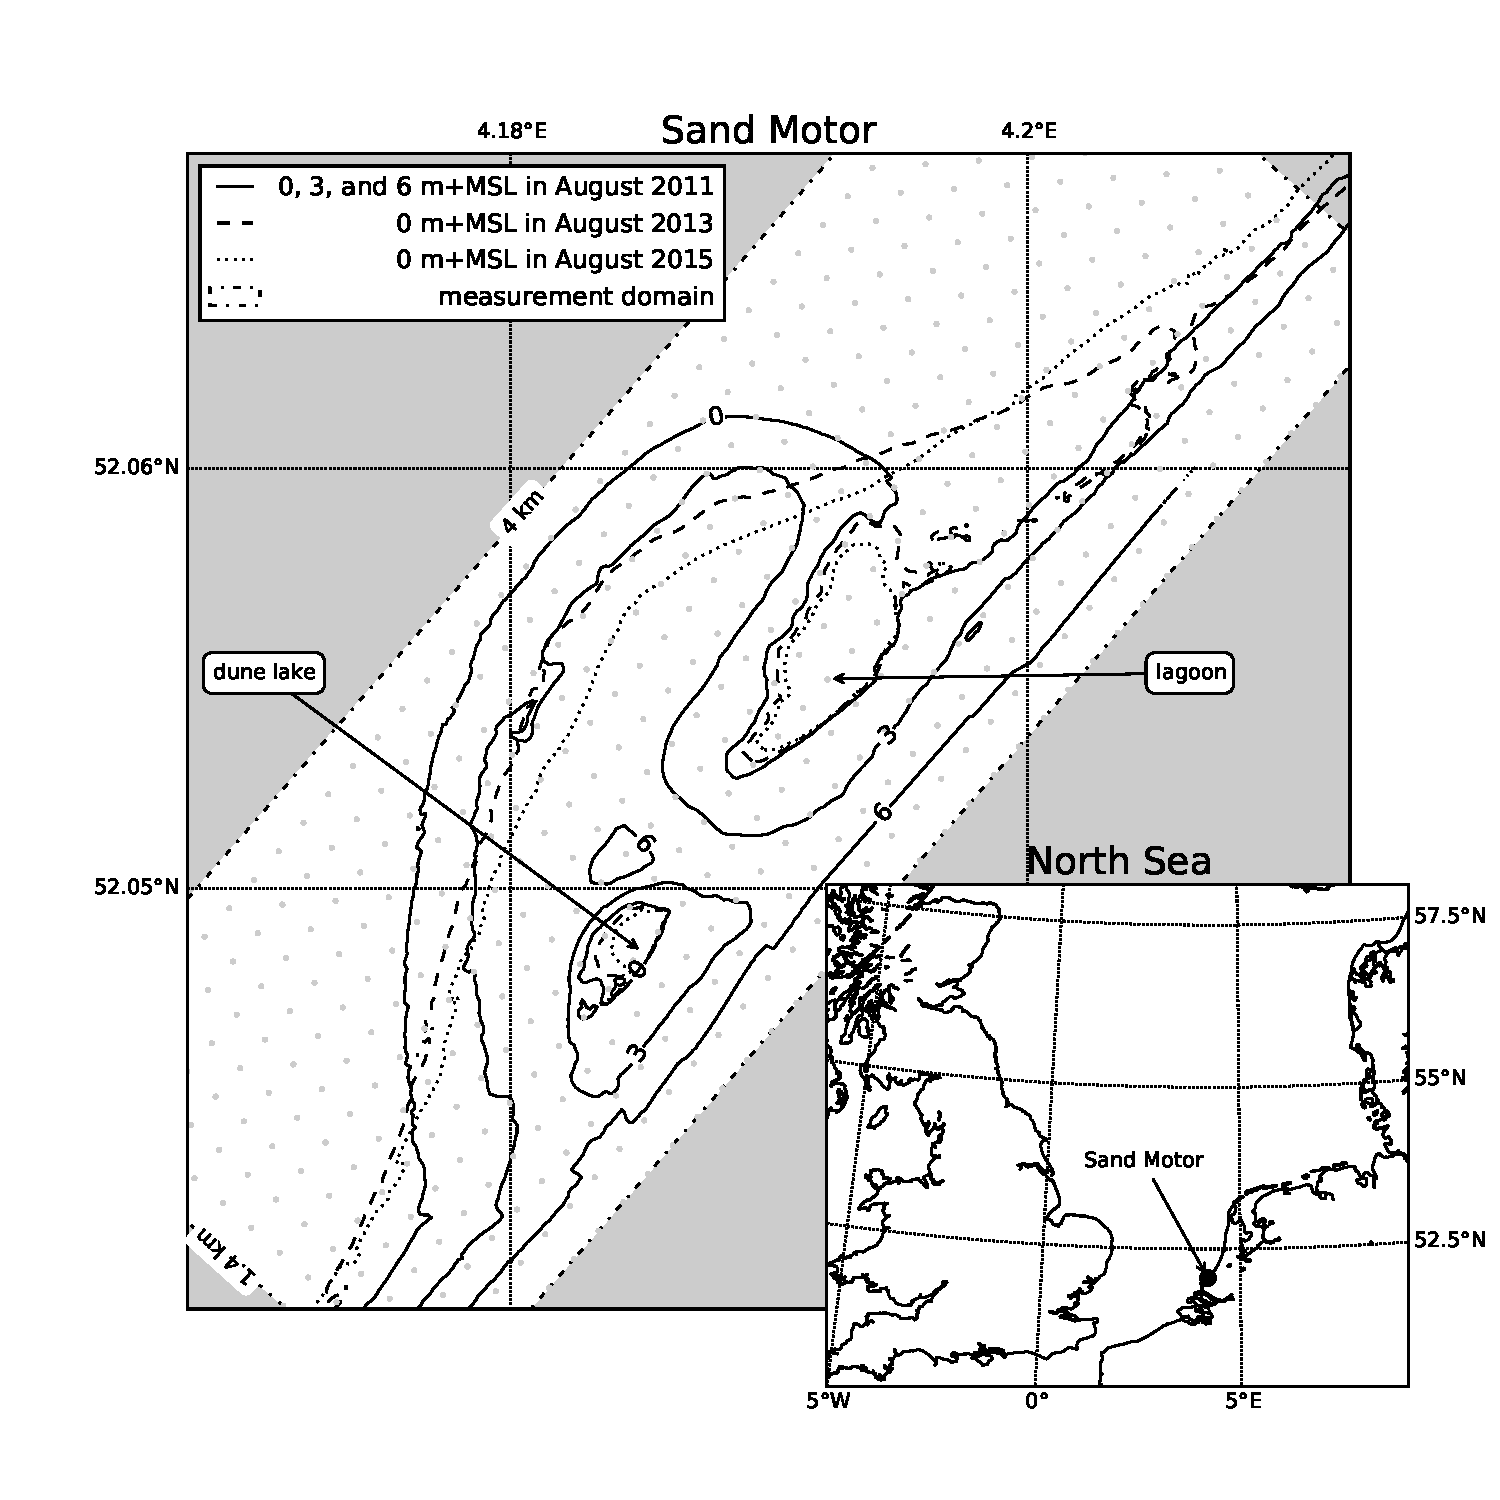
\includegraphics[width=\columnwidth]{../Figures/location_and_evolution}
  \caption{Location, orientation, appearance and evolution of the Sand
    Motor between construction in 2011 and 2015. The box indicates the
    measurement domain used in the remainder of this paper. A 100 x
    100 m grid aligned with the measurement domain is plotted in gray
    as reference.}
  \label{fig:fieldsite3}
\end{figure}

Due to natural sediment dynamics the Sand Motor distributes about 1
$\mathrm{Mm^3}$ of sand per year to the adjacent coasts (Figure
\ref{fig:fieldsite3}). The majority of this sand volume is transported
by tides and waves. However, the Sand Motor is constructed up to 5
m+MSL and locally up to 7 m+MSL, which is in either case well above
the maximum surge level of 3 m+MSL (Figure
\ref{fig:boundaryconditions}c). Therefore, the majority of the Sand
Motor area is uniquely shaped by wind.

The Sand Motor comprises both a dune lake and a lagoon that act as
large traps for aeolian sediment (Figure \ref{fig:fieldsite3}). The
lagoon is affected by tidal forcing, although the tidal amplitude
quickly diminished over time as the entry channel elongated. The tidal
range of about 2 m that is present at the Sand Motor periphery (Figure
\ref{fig:boundaryconditions}c), is nowadays damped to less than 20 cm
inside the lagoon \citep{deVries2015}. Consequently, the tidal
currents at the closed end of the lagoon, where most aeolian sediment
is trapped, are negligible.

%Sand used for construction of the Sand Motor is obtained from an
%offshore borrowing pit in the North Sea. The sand is predominantly
%Holocene sand with a significant amount of fines. The median grain
%size is slightly coarser than found originally along the Delfland
%coast. Apart from sand fractions, the sediment contains a large amount
%of shells, shell fractions, some pebbles and cobbles and an occasional
%fraction of a mammoth bone.

%\begin{figure}
%  \centering
%  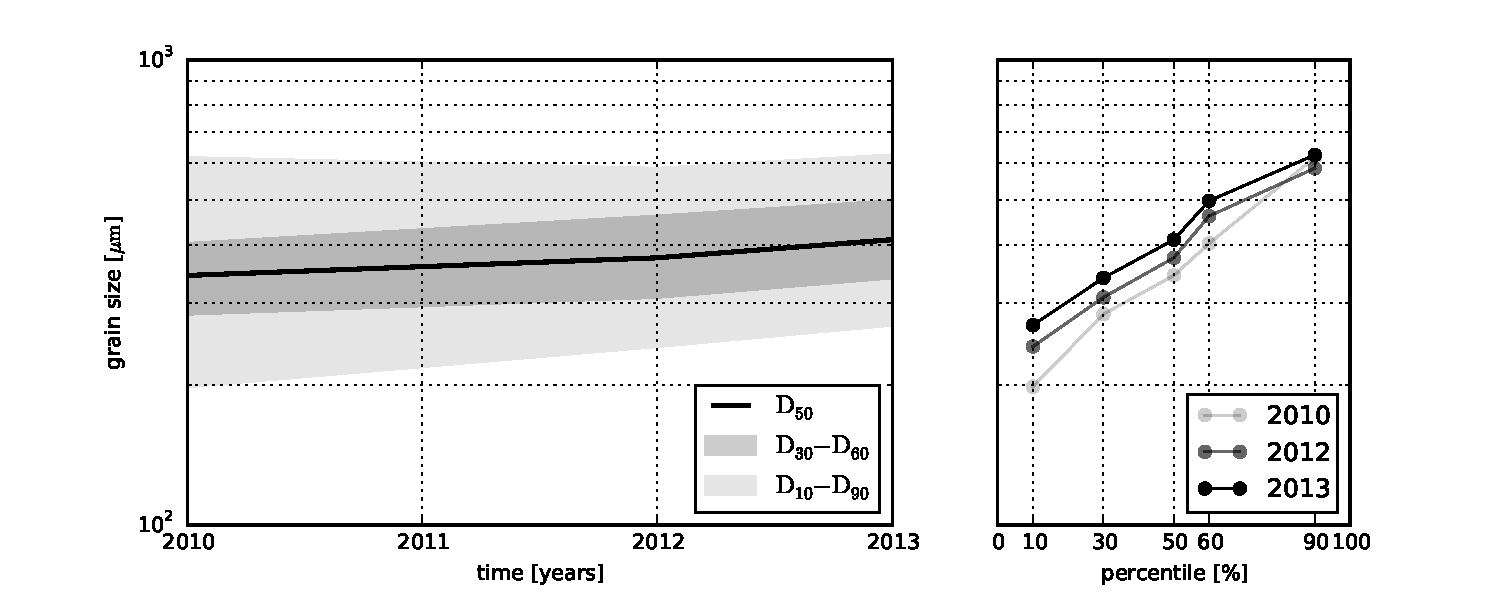
\includegraphics[width=\columnwidth]{../Figures/grainsize}
%  \caption{Evolution of the grain size distribution at the dry beach
%    since 2010, prior to construction of the Sand Motor
%    \citep{ImaresSamples}. Left panel: time series of median grain
%    size. Right panel: grain size distributions.}
%  \label{fig:grainsize}
%\end{figure}

The dominant wind direction at the Sand Motor is south to southwest
(Figure \ref{fig:boundaryconditions}a). However, during storm
conditions the wind direction tends to be southwest to
northwest. During extreme storm conditions the wind direction tends to
be northwest. Northwesterly storms are typically accompanied by
significant surges as the fetch is virtually unbounded to the
northwest, while surges from the southwest are limited due to the
presence of the narrowing of the North Sea at the Strait of Dover
(Figure \ref{fig:fieldsite3}, inset).

\begin{figure}
  \centering
  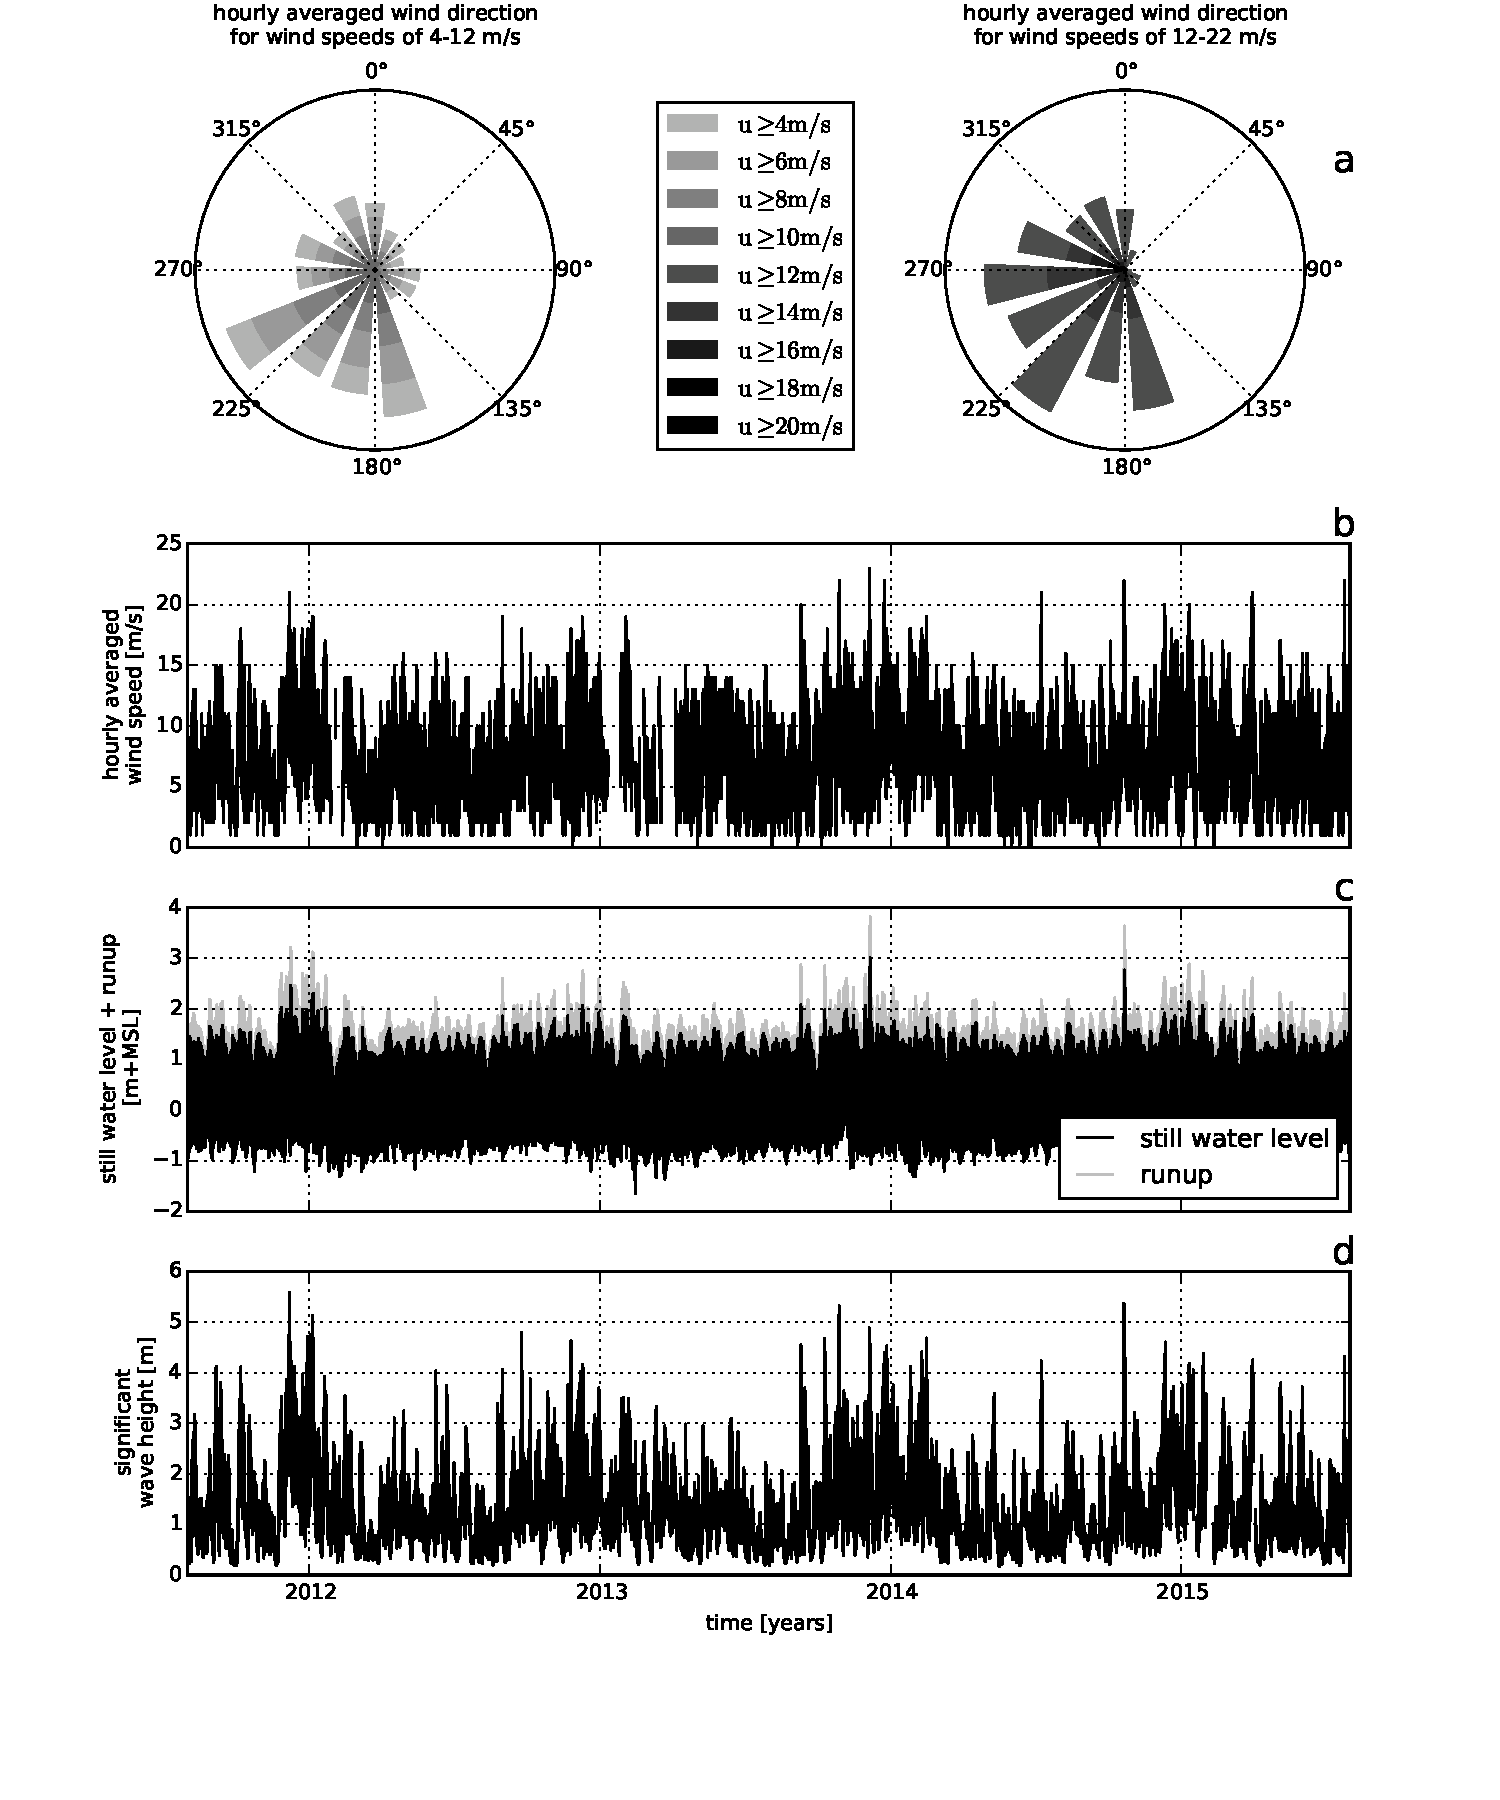
\includegraphics[width=\columnwidth]{../Figures/boundaryconditions}
  \caption{Wind and hydrodynamic time series from 2011 to 2015. Hourly
    averaged wind speeds and directions are obtained from the KNMI
    meteorological station in Hoek van Holland (upper
    panels). Offshore still water levels, wave heights and wave
    periods are obtained from the Europlatform (lower panels). Runup
    levels are estimated following \citet{Stockdon2006}.}
  \label{fig:boundaryconditions}
\end{figure}

%\section{Sediment transport capacity}
%\label{sec:transport_capacity}
%
%\begin{figure}
%  \centering
%  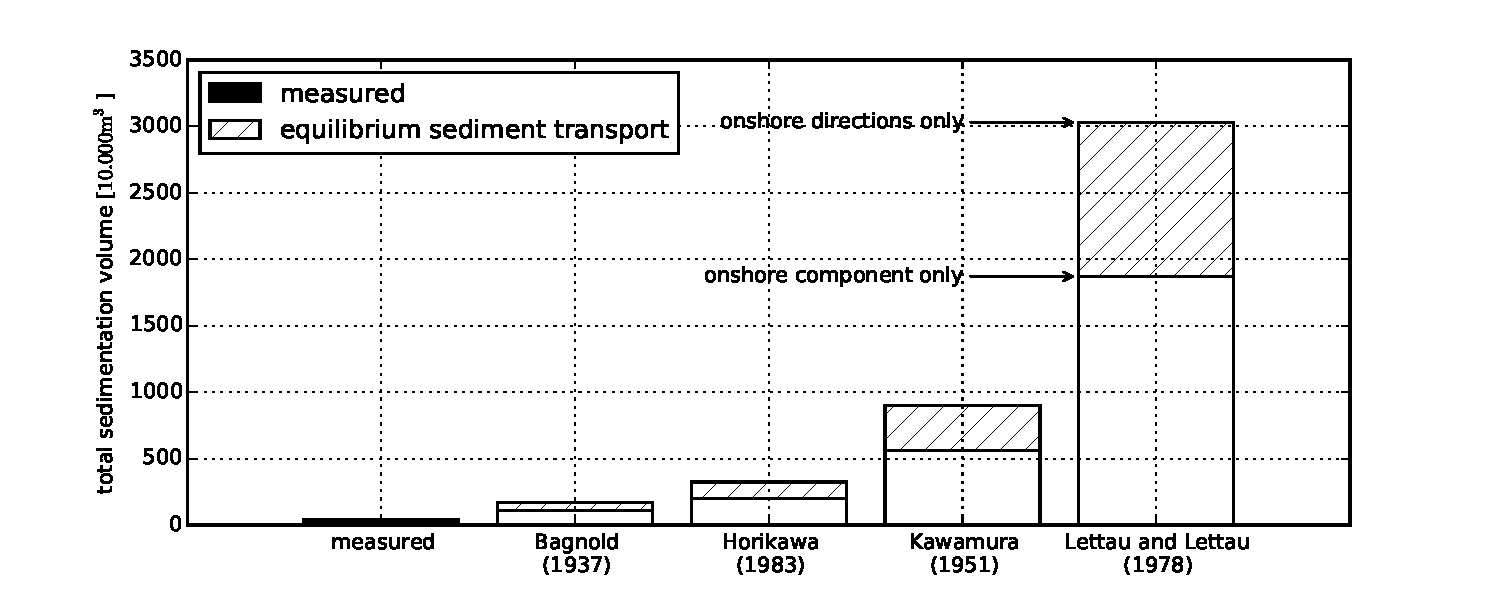
\includegraphics[width=\columnwidth]{../Figures/transport_models}
%  \caption{Comparison of the cumulative aeolian sediment transport
%    capacity according to a selection of equilibrium sediment
%    transport formulations and measured total sedimentation in the
%    Sand Motor region (upper panel). The sediment transport capacity
%    is based on an hourly averaged wind speed and direction time
%    series from September 1, 2011 until September 1, 2015. Offshore
%    wind directions are discarded. For the upper boundary of each
%    estimate all wind directions are weighted equally. For the lower
%    boundary of each estimate the wind directions are weighted
%    according to the magnitude of the onshore component. All
%    formulations overestimate the measured sedimentation volume
%    significantly. The \textsc{AeoLiS} model uses the formulation from
%    \citet{Bagnold1937a} and therefore produces comparable results if
%    all availability limiting processes are disabled (lower
%    panel). The shaded area in the lower panel is a detailed view on
%    the shaded area in the upper panel.}
%  \label{fig:models}
%\end{figure}
%
%The Sand Motor is an availability-limited system as measured aeolian
%sediment transport rates are consistently lower than the sediment
%transport capacity. The sediment transport capacity is described by
%equilibrium sediment transport formulations. Figure \ref{fig:models}
%(upper panel) presents an overview of the cumulative sediment
%transport capacity (or potential sediment accumulation) at the Sand
%Motor over the period between September 1, 2011 and September 1, 2015
%according to a selection of equilibrium sediment transport
%formulations. The cumulative sediment transport capacity $Q$
%[$\mathrm{m^3}$] is estimated based on hourly averaged time series of
%the wind speed $u_z$ [m/s] and direction $\theta_u$ [$^{\circ}$]
%obtained from the KNMI meteorological station in Hoek van Holland
%following:
%
%\begin{equation}
%  \label{eq:transport_capacity}
%  Q = \sum q \cdot f_{\theta_u} \cdot \frac{\Delta t \cdot \Delta y}{(1 - p) \cdot \rho_{\mathrm{p}}}
%\end{equation}
%
%\noindent where $\Delta t$ = 1 h, $\Delta y$ = 4 km, $p$ = 0.4,
%$\rho_{\mathrm{p}}$ = 2650 $\mathrm{kg/m^3}$, $q$ is given by the
%equilibrium sediment transport formulation (Table \ref{tab:models})
%and $f_{\theta_u}$ is a factor to account for the wind direction.
%
%\begin{table}
%  \centering
%  \caption{Equilibrium sediment transport formulations and coefficient values. 
%    Other values are $u_{\mathrm{*}} = \alpha \cdot u_z$ m/s, $u_{\mathrm{* th}} = \alpha \cdot 3.87$ m/s,
%    $\alpha = 0.058$, $\rho_{\mathrm{a}}$ = 1.25 $\mathrm{kg/m^3}$,
%    $\rho_{\mathrm{p}}$ = 2650.0 $\mathrm{kg/m^3}$, $g$ = 9.81
%    $\mathrm{m/s^2}$, $d_{\mathrm{n}}$ = 335 $\mu \mathrm{m}$, 
%    $D_{\mathrm{n}}$ = 250 $\mu \mathrm{m}$ and
%    $z$ = 10 m.}
%  \label{tab:models}
%  \begin{tabular}{lll}
%    Reference & Equation & $C$ \\
%    \hline
%    \citet{Bagnold1937a} & $q = C \frac{\rho_{\mathrm{a}}}{g} \sqrt{\frac{d_{\mathrm{n}}}{D_{\mathrm{n}}}} \left(u_{\mathrm{*}} - u_{\mathrm{* th}} \right)^3$ & 1.8 \\
%    \citet{Horikawa1983} & \multirow{2}{*}{$q = C \frac{\rho_{\mathrm{a}}}{g} \left(u_{\mathrm{*}} + u_{\mathrm{* th}} \right)^2 \left(u_{\mathrm{*}} - u_{\mathrm{* th}} \right)$} & 1.0 \\
%    \citet{Kawamura1951} &  & 2.78 \\
%    \citet{Lettau1978} & $q = C \frac{\rho_{\mathrm{a}}}{g} \sqrt{\frac{d_{\mathrm{n}}}{D_{\mathrm{n}}}} \left(u_{\mathrm{*}} - u_{\mathrm{* th}} \right) u_{\mathrm{*}}^2$ & 6.7 \\
%  \end{tabular}
%\end{table}
%
%The wind direction can be accounted for by only including the onshore
%wind component. However, given the typical Sand Motor topography,
%sediment is likely to be trapped in the dune lake and lagoon even
%without a cross-shore wind component (alongshore wind). Therefore it
%can be assumed that the onshore wind component will provide a lower
%limit of the cumulative sediment transport capacity in the Sand Motor
%region. Similarly, an upper limit can be obtained by assuming that all
%onshore wind directions contribute equally to the cumulative sediment
%transport capacity in the Sand Motor region. For the upper limit the
%factor $f_{\theta_u}$ is defined as:
%
%\begin{equation}
%  f_{\theta_u} = \left\{
%      \begin{array}{rcl}
%        1 & \mathrm{if} & \cos \left( \theta_u + 48\,^{\circ} \right) \geq 0 \\
%        0 & \mathrm{if} & \cos \left( \theta_u + 48\,^{\circ} \right) < 0 \\
%      \end{array}
%    \right.
%\end{equation}
%
%\noindent while for the lower limit the factor $f_{\theta_u}$ is defined
%as:
%
%\begin{equation}
%  f_{\theta_u} = \max \left( 0 \quad ; \quad \cos \left( \theta_u + 48\,^{\circ} \right) \right)
%\end{equation}
%
%The estimates for the sediment transport capacity show a large
%variability depending on the equilibrium sediment transport
%formulation used. The variations correspond well to the evaluations
%presented by \citet{Sherman2012} and suggest that the
%\citet{Bagnold1937a} formulation is relatively accurate. In addition,
%it is the only formulation that is suitable for multi-fraction aeolian
%sediment transport as it is derived separately for different grain
%sizes. The formulation from \citet{Bagnold1937a} is therefore selected
%for the \textsc{AeoLiS} model (Equation \ref{eq:erodep} and
%\ref{eq:equilibrium_transport}).
%
%Figure \ref{fig:models} (lower panel) shows a comparison between the
%measured sediment accumulation in the Sand Motor region, the estimates
%based on the \citet{Bagnold1937a} formulation and a preliminary
%simulation with the \textsc{AeoLiS} model in which availability
%limiting processes are disabled. The result confirms that the model
%follows the equilibrium sediment transport rate when sediment
%availability and fetch are not limited. Moreover, the result suggests
%that limitations in sediment availability reduces the sediment
%accumulation with 75\%, which is close to the upper limit of the range
%64\% -- 76\% estimated with the equilibrium sediment transport
%formulation alone.

\section{Model approach}

% link to sediment transport capacity
% link to specific results from chapter 2 for hindcast

A two-dimensional (2DH) model of the Sand Motor that includes
limitations in sediment availability is constructed and calibrated
based on four years of field measurements on wind, tides, waves and
topography. The calibrated model is used to investigate the influence
of spatiotemporal variations in aeolian sediment availability on
sediment accumulation in the Sand Motor domain.

To test that the Sand Motor mega nourishment is indeed an
availability-limited coastal system, the measured long-term sediment
accumulation volumes \citep{Hoonhout2017a} are first compared to a
reference model that assumes no limitations in sediment availability
exist.

%A numerical model of the Sand Motor region is constructed and
%calibrated for the period between September 1, 2011 and September 1,
%2015 as to investigate the influence of sediment availability on
%aeolian sediment transport rates. The sediment availability at the
%Sand Motor seems to be governed in particular by soil moisture content
%and beach armoring (Chapter \ref{ch:largescale} and
%\ref{ch:smallscale}). Therefore the calibration focuses on the drying
%rate of the soil after flooding and the sheltering of the sand surface
%by roughness elements emerging from the bed.
%
%The model presented in Chapter \ref{ch:model} is extended to obtain a
%representation of the hydrodynamic forcing that is sufficiently
%accurate for the Sand Motor hindcast. As the Sand Motor accommodates a
%dune lake, lagoon and a rapidly changing contour, large spatial
%variations in hydrodynamic forcing are present in the Sand Motor
%region. These spatial variations are largely disregarded by the model
%presented in Chapter \ref{ch:model}. Moreover, the significant
%topographic changes induced by hydrodynamic forcing are ignored.

%The calibrated model is applied to the period between September 1,
%2015 and September 1, 2016 as to test the predictive capabilities of
%the model. Testing to model on a period that has not been used for
%calibration aims at a test result independent of calibration. As
%insufficient measurements on the bed composition are available, the
%final bed composition from the calibration run is used as initial bed
%composition in the test run.

\subsection{Reference model}

\begin{figure}
  \centering
  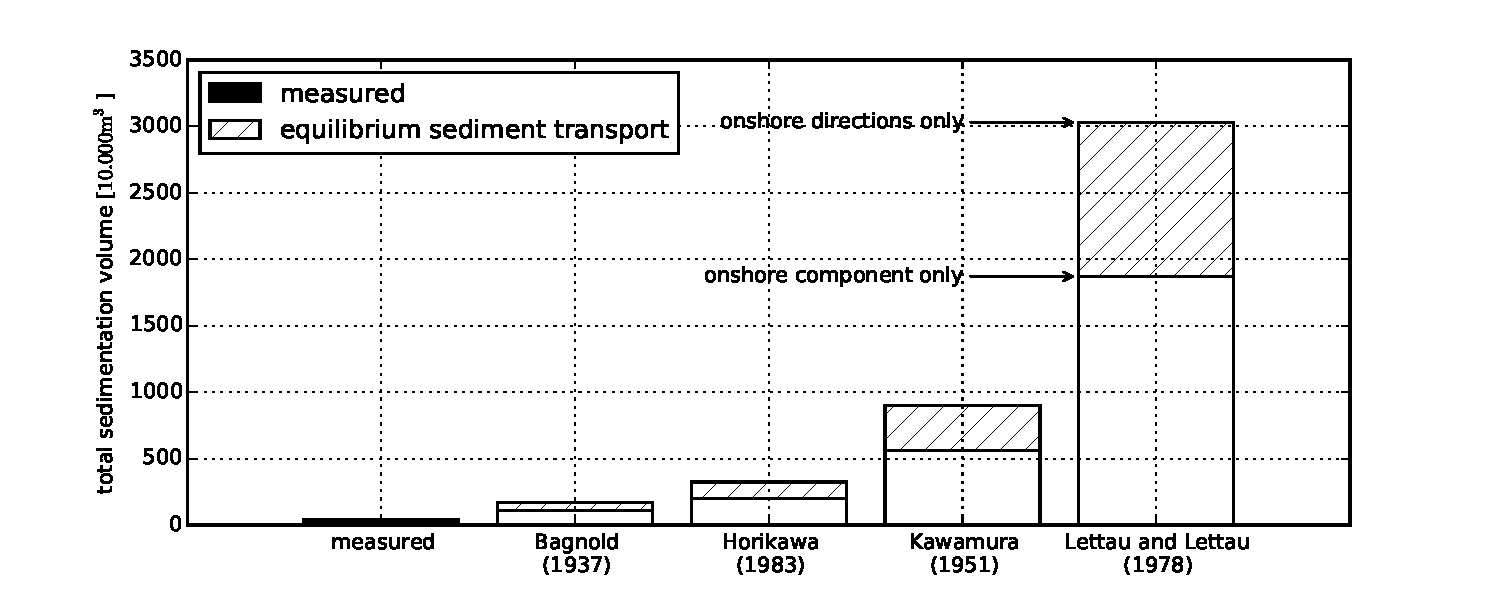
\includegraphics[width=\columnwidth]{../Figures/transport_models}
  \caption{Comparison of the cumulative wind transport capacity
    according to a selection of equilibrium sediment transport
    formulations and measured total sedimentation in the Sand Motor
    domain. The equilibrium sediment transport is based on an hourly
    averaged wind speed and direction time series from September 1,
    2011 until September 1, 2015. Offshore wind directions are
    discarded. For the upper boundary of each estimate all wind
    directions are weighted equally. For the lower boundary of each
    estimate the wind directions are weighted according to the
    magnitude of the onshore component.}
  \label{fig:models}
\end{figure}

A selection of equilibrium sediment transport formulations is used as
reference model. An equilibrium sediment transport formulation
describes the wind transport capacity in given conditions. In
conjunction with a shear velocity threshold based on only a constant
uniform median grain size, an estimate of the potential aeolian
sediment accumulation in absence of availability-limitations can be
obtained. The potential aeolian sediment accumulation or cumulative
wind transport capacity $Q$ [$\mathrm{m^3}$] in the Sand Motor domain
is estimated based on hourly averaged time series of the wind speed
$u_z$ [m/s] and direction $\theta_u$ [$^{\circ}$] obtained from the
KNMI meteorological station in Hoek van Holland following:

\begin{equation}
  \label{eq:transport_capacity}
  Q = \sum q \cdot \frac{\Delta t \cdot \Delta y}{(1 - p) \cdot \rho_{\mathrm{p}}} \cdot f_{\theta_u}
\end{equation}

\noindent where the temporal resolution $\Delta t$ = 1 h, the
alongshore span of the domain $\Delta y$ = 4 km, the porosity $p$ =
0.4, the particle density $\rho_{\mathrm{p}}$ = 2650
$\mathrm{kg/m^3}$, the sediment transport rate $q$ is given by the
equilibrium sediment transport formulation (Table \ref{tab:models})
and $f_{\theta_u}$ is a factor to account for the wind direction. The
wind direction can be accounted for by only including the onshore wind
component with respect to the original coastline orientation. However,
given the typical Sand Motor geometry (Figure \ref{fig:fieldsite3}),
sediment is likely to be trapped in the dune lake and lagoon even with
alongshore wind. Therefore it can be assumed that the onshore wind
component will provide a lower limit of the cumulative wind transport
capacity. Similarly, an upper limit can be obtained by assuming that
all onshore wind directions contribute equally to the cumulative wind
transport capacity. For the upper limit the factor $f_{\theta_u}$ is
defined as:

\begin{equation}
  f_{\theta_u} = \left\{
      \begin{array}{rcl}
        1 & \mathrm{if} & \cos \left( 312\,^{\circ} - \theta_u \right) \geq 0 \\
        0 & \mathrm{if} & \cos \left( 312\,^{\circ} - \theta_u \right) < 0 \\
      \end{array}
    \right.
\end{equation}

\noindent while for the lower limit the factor $f_{\theta_u}$ is defined
as:

\begin{equation}
  f_{\theta_u} = \max \left( 0 \quad ; \quad \cos \left( 312\,^{\circ} - \theta_u \right) \right)
\end{equation}

\noindent where $312\,^{\circ}$ accounts for orientation of the original
coastline.  Figure \ref{fig:models} presents an overview of the
cumulative wind transport capacity in the Sand Motor domain over the
period between September 1, 2011 and September 1, 2015 according to a
selection of equilibrium sediment transport formulations and in
comparison with the measured accumulation volumes. The estimates of
the wind transport capacity show a large variation between
formulations that are mainly due to the incorporation of the shear
velocity threshold. However, all formulations overestimate the
measured sediment accumulation in the Sand Motor domain with at least
a factor 3 -- 4. The large variation and consistent overestimation is
in accordance with the review of aeolian sediment transport models
presented by \citet{Sherman2012}. The consistent overestimation of the
measured sedimentation volumes in the Sand Motor domain suggest that
the Sand Motor is indeed an availability-limited coastal system.

\subsection{Schematization}

\begin{figure}
  \centering
  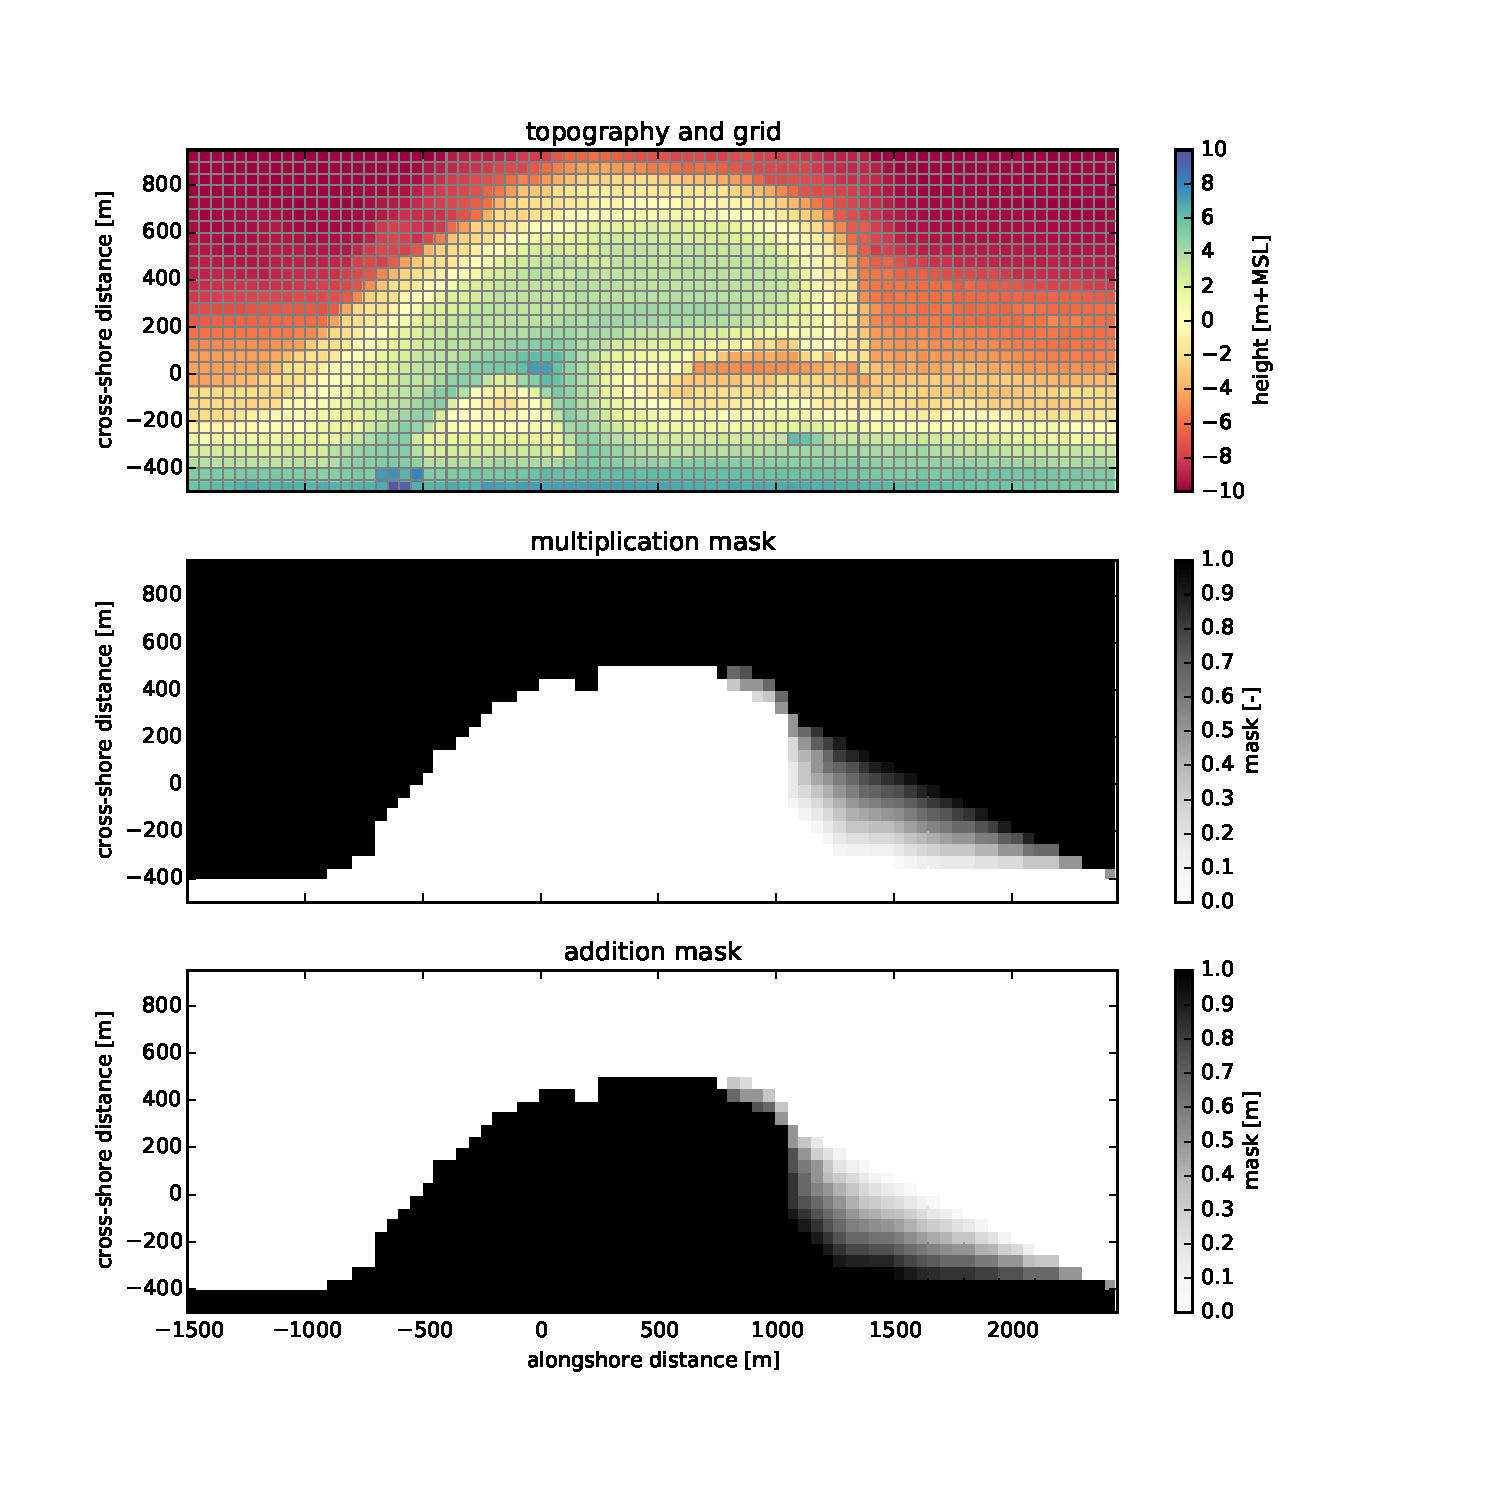
\includegraphics[width=\columnwidth]{../Figures/gridmask}
  \caption{Model grid and topography based on the topographic survey
    of August 3, 2011 (upper panel) and hydrodynamic mask used to
    limit tidal and wave motions in the dune lake and lagoon (middle
    and lower panels). Water levels and wave heights are uniformly
    imposed to the model and multiplied by the multiplication mask and
    subsequently increased with the addition mask.}
  \label{fig:gridmask}
\end{figure}

%\begin{figure}
%  \centering
%  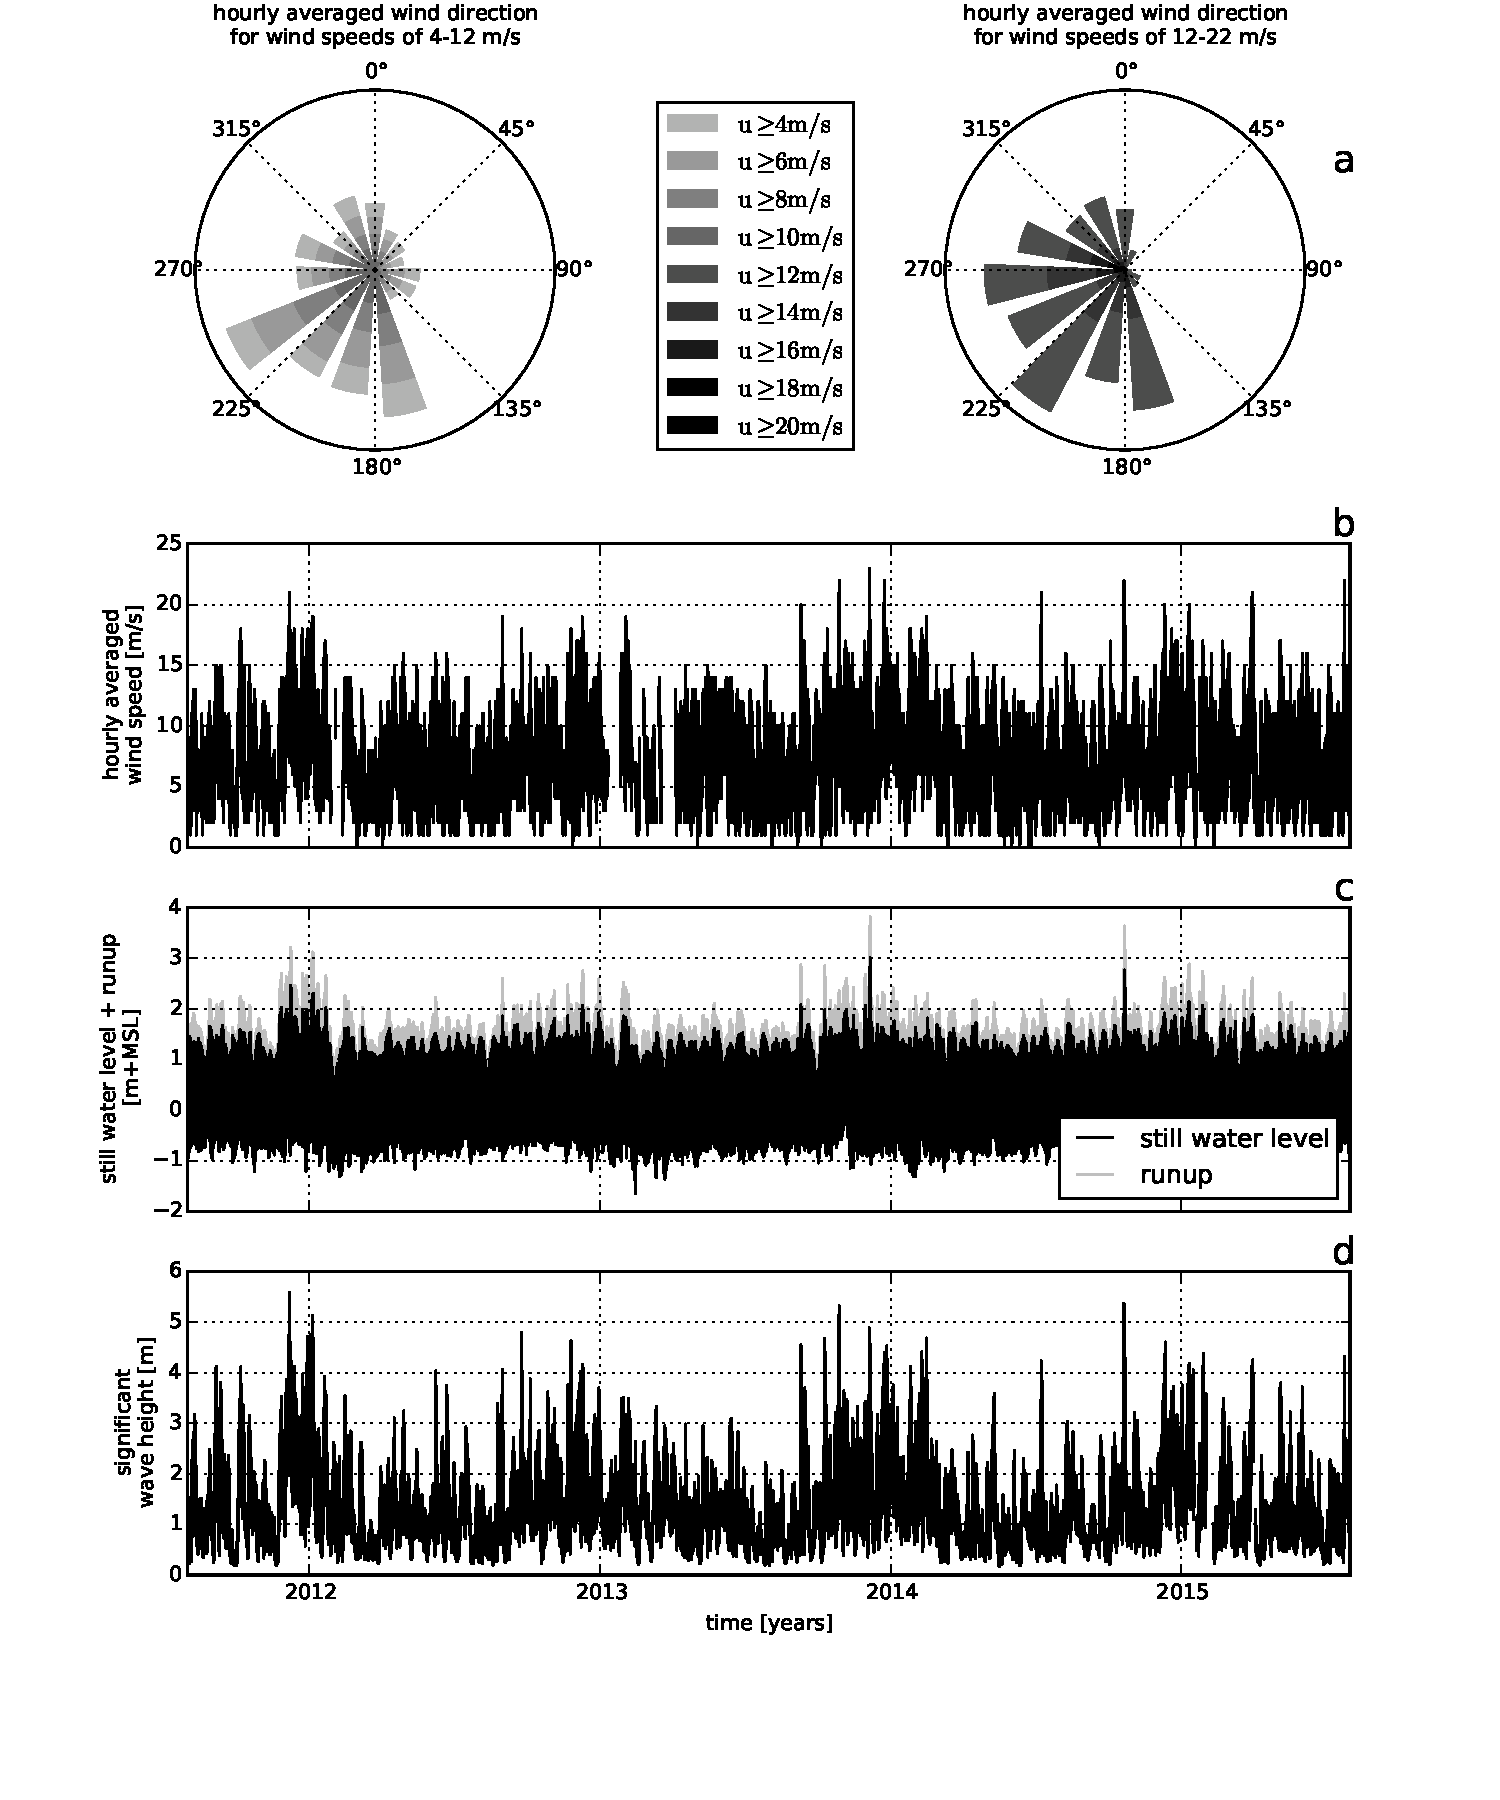
\includegraphics[width=\columnwidth]{../Figures/boundaryconditions}
%  \caption{Wind and hydrodynamic boundary conditions imposed to the
%    model. Hourly averaged wind speeds and directions are obtained
%    from the KNMI meteorological station in Hoek van Holland (upper
%    panels). Offshore still water levels, wave heights and wave
%    periods are obtained from the Europlatform (lower panels). Runup
%    levels are estimated following \citet{Stockdon2006}.}
%  \label{fig:boundaryconditions}
%\end{figure}

% topography and grid
A two-dimensional (2DH) aeolian sediment availability and transport
model for the Sand Motor mega nourishment is constructed for the four
years between September 1, 2011 and September 1, 2015, which is
shortly after the nourishment was placed. The model's topography and
grid are based on the measured topographies of August 3, 2011 and
later. The topographies are rotated $48\,^{\circ}$ and interpolated to
a 50 x 50 m grid spanning 1.5 km cross-shore and 4 km alongshore with
respect to the original coastline, not including the dunes (Figure
\ref{fig:gridmask}, upper panel).

% boundary conditions
Four years of hourly wind speed and direction data measured at 10 m
above the bed is obtained from the KNMI meteorological station at Hoek
van Holland (Figure \ref{fig:boundaryconditions}a,b). Hourly offshore
water levels and wave heights are obtained from the Europlatform for
the same period (Figure \ref{fig:boundaryconditions}c,d).

% grain size and shells, layers and layer thickness
An average lognormal grain size distribution with a median diameter
$d_{50} = 335 ~ \mu \mathrm{m}$ is used as measured at the Sand Motor
field site. The sand fractions cover a range from 0.1 to 2 mm. The
amount of shells and other roughness elements in the originally
nourished sand is estimated to be 5\%. The estimate is based on three
sediment samples obtained from the field site 0.5 m below the bed
surface. Additional fractions ranging from 2 to 32 mm are added
according to a lognormal distribution to account for the presence of
roughness elements in the bed. The grain size distribution is used to
populate the initial bed that consists of 10 bed composition layers
with a thickness of 1 cm each.

% timestep and scheme
The hindcast aims at the large scale and long term sedimentation
volumes as presented by \citet{Hoonhout2016a}. Therefore an efficient,
but diffusive, implicit Euler Backward scheme with a timestep of 1 h
is used that does not resolve high frequency variations in wind or
sediment transport. Consequently, the model produces smooth solutions
that describe hourly steady states based on the instantaneous average
wind speed and sediment availability.

% equilibrium sediment transport formulation

\begin{table}
  \centering
  \caption{Equilibrium sediment transport formulations, coefficient
    values* and the ratio between measurements and model results.}
  \label{tab:models}
  \begin{tabular}{llll}
    Reference & Equation & $C$ & Ratio \\
    \hline
    \citet{Bagnold1937a} & $q = C \frac{\rho_{\mathrm{a}}}{g} \sqrt{\frac{d_{\mathrm{n}}}{D_{\mathrm{n}}}} \left(u_{\mathrm{*}} - u_{\mathrm{* th}} \right)^3$ & 1.8 & 3 -- 4 \\
    \citet{Horikawa1983} & \multirow{2}{*}{$q = C \frac{\rho_{\mathrm{a}}}{g} \left(u_{\mathrm{*}} + u_{\mathrm{* th}} \right)^2 \left(u_{\mathrm{*}} - u_{\mathrm{* th}} \right)$} & 1.0 & 5 -- 8 \\
    \citet{Kawamura1951} &  & 2.78 & 14 -- 22 \\
    \citet{Lettau1978} & $q = C \frac{\rho_{\mathrm{a}}}{g} \sqrt{\frac{d_{\mathrm{n}}}{D_{\mathrm{n}}}} \left(u_{\mathrm{*}} - u_{\mathrm{* th}} \right) u_{\mathrm{*}}^2$ & 6.7 & 46 -- 75 \\
  \end{tabular}

  \footnotesize{
    \begin{enumerate}[{*}]
    \item Other values are the shear velocity
      $u_{\mathrm{*}} = \alpha \cdot u_z$ m/s, the shear velocity
      threshold $u_{\mathrm{* th}} = \alpha \cdot 3.87$ m/s, the
      conversion factor from free-flow wind velocity to shear velocity
      $\alpha = 0.058$, the air density $\rho_{\mathrm{a}}$ = 1.25
      $\mathrm{kg/m^3}$, the particle density $\rho_{\mathrm{p}}$ =
      2650.0 $\mathrm{kg/m^3}$, the gravitational constant $g$ = 9.81
      $\mathrm{m/s^2}$, the nominal grain size $d_{\mathrm{n}}$ = 335
      $\mu \mathrm{m}$, a reference grain size $D_{\mathrm{n}}$ = 250
      $\mu \mathrm{m}$ and the height above the bed of the wind
      measurement $z$ = 10 m.
    \end{enumerate}
  }
\end{table}

\citet{Bagnold1937a} is selected as equilibrium sediment transport
formulation as it is derived separately for different grain sizes and
therefore suitable for multi-fraction aeolian sediment
transport. Alternative formulations (Table \ref{tab:models}) are
derived for wider grain size distributions that do not necessarily
result in a monotonic relation between the grain size and the sediment
transport rate \citep[e.g.][]{Kawamura1951, Horikawa1983}. Such
non-monotonic relation is unrealistic in a multi-fraction context as
it would result in a preference to transport both fine sediment and
large elements that are considered non-erodible. Moreover, the
formulation of \citet{Bagnold1937a} overestimates the measured aeolian
sediment transport rates in the Sand Motor domain less compared to
alternative formulations (Table \ref{tab:models}, rightmost column).

% masks
Water levels and wave heights are initially uniformly imposed to the
model. Consequently, the tidal range, mean water level and wave
heights that are present at the Sand Motor periphery are also present
in the dune lake and lagoon. In reality the tidal range and wave
heights in the dune lake and lagoon are much lower, while the mean
water level in the dune lake and lagoon is elevated compared to mean
sea level \citep{deVries2015}. To account for these spatial
differences in hydrodynamics a hydrodynamic mask is applied (Figure
\ref{fig:gridmask}, middle and lower panel; Appendix \ref{apx:mask})

% BMI
Subtidal changes in topography are not simulated by the model. The
subtidal changes can be important to aeolian sediment transport as the
location and size of aeolian sediment erosion and deposition areas
might change. To account for these changes, measured topographies are
imposed to the model through a Basic Model Interface
\citep[BMI,][Appendix \ref{apx:bmi}]{Peckham2013}.

All measured topographies in the period between September 1, 2011 and
September 1, 2015 are linearly interpolated in time as to obtain daily
updates of the Sand Motor's topography. The hydrodynamic mask is
updated along with the topography. The presented aeolian sediment
transport rates are based on the time-integrated entrainment and
deposition rates that are computed by the model rather than
differences in topography.

\subsection{Calibration}

The model is calibrated on the shape of roughness elements that emerge
from the bed and shelter the sand surface from wind erosion, the
drying rate of the soil and the time needed for the sediment transport
to adapt to changing wind conditions. These processes are represented
in the model by parameters for which data or literature can only
provide approximate values:

\begin{enumerate}
\item $\sigma$, as used in the formulation of \citet[][Equation
  \ref{eq:raupach}]{Raupach1993}, is the ratio between the basal and
  frontal area of the roughness elements that constitute the beach
  armor layer.
\item $T_{\mathrm{dry}}$ is the time scale at which the beach dries
  out after flooding (Equation \ref{eq:apx_drying}). It represents the
  time in which the soil moisture content halves in case the beach is
  not inundated and no evaporation occurs.
\item $T$ is the adaptation time scale in the right-hand side of the
  advection equation (Equation \ref{eq:erodep}). It represents the
  time scale to which the sediment transport adapts to variations in
  the wind conditions and sediment availability.
\end{enumerate}

% Wind tunnel experiments presented by \citet{McKennaNeuman2012}
% provide leads on appropriate values for $\sigma$. The wind tunnel
% experiments investigated the influence of a beach armor layer,
% consisting of shells and shell fragments, on aeolian sediment
% transport. The results were used to derive optimal values for the
% parameters $\sigma$ and $\beta$ (Equation \ref{eq:raupach}).

The implementation of roughness elements is characterized by three
calibration parameters: $m$, $\beta$ and $\sigma$ (Equation
\ref{eq:raupach2}). $m$ is a factor to account for the difference
between the mean and maximum shear stress and is usually chosen as 0.5
for field applications \citep{Raupach1993,
  McKennaNeuman2012}. Numerically it is irrelevant if $\beta$ or
$\sigma$ is calibrated as they only appear as a ratio
$\frac{\beta}{\sigma}$ in the model implementation. As $\beta$ is the
ratio between the drag coefficient of the roughness elements alone and
the drag coefficient of the unarmored sandy bed, the value can be
assumed to be reasonably generic. In contrast, $\sigma$ depends on the
shape and protrusion of the roughness elements and therefore depends
on the field site and varies in time. For example, a spherical object
placed on top of the bed would be represented by $\sigma = 1$, while a
spherical object protruding halfway through the bed (hemisphere) would
be represented by $\sigma = 2$. Consequently, calibration of $\sigma$
seems to be preferable as it is less certain. Wind tunnel experiments
presented by \citet{McKennaNeuman2012} investigated the influence of a
lag deposits, consisting of shells and shell fragments, on aeolian
sediment transport. Values for the calibration coefficients $m$ and
$\beta$ were found to be 0.5 and 130 respectively and are adopted for
the Sand Motor hindcast. An optimal average value for $\sigma$ is
obtained by systematic variation between 2 and 20.

The drying rate of the beach ($T_{\mathrm{dry}}$) depends on many
factors, like grain size, soil moisture content, groundwater level,
wind speed and solar radiation. The use of a single time scale as
aggregate for these processes is an oversimplification of
reality. Therefore a wide range of parameter values is covered in the
calibration. $T_{\mathrm{dry}}$ is varied between 0.1 and 10 hours
where the former results in virtually instant drying and the latter
results in an intertidal beach that is permanently too moist for
aeolian sediment transport to be initiated.

The adaptation time scale ($T$), that represents the swiftness of
aeolian sediment transport to adapt to changing wind conditions, is in
the order of seconds \citep{DavidsonArnott2008, deVries2014a}. As the
model time step is orders of magnitude larger, the model effectively
solves steady states and the value for $T$ will not affect temporal
variations in sediment transport. However, the adaptation time scale
also affects the development of the saltation cascade in
space. Sediment transport increases in downwind direction from a
zero-flux boundary, like the water line in case of onshore wind, with
a rate that is governed by the value of $T$. Consequently, $T$
influences the width of the source area in case of abundant sediment
availability. $T$ is varied between 1 and 10 seconds.

\begin{figure}
  \centering
  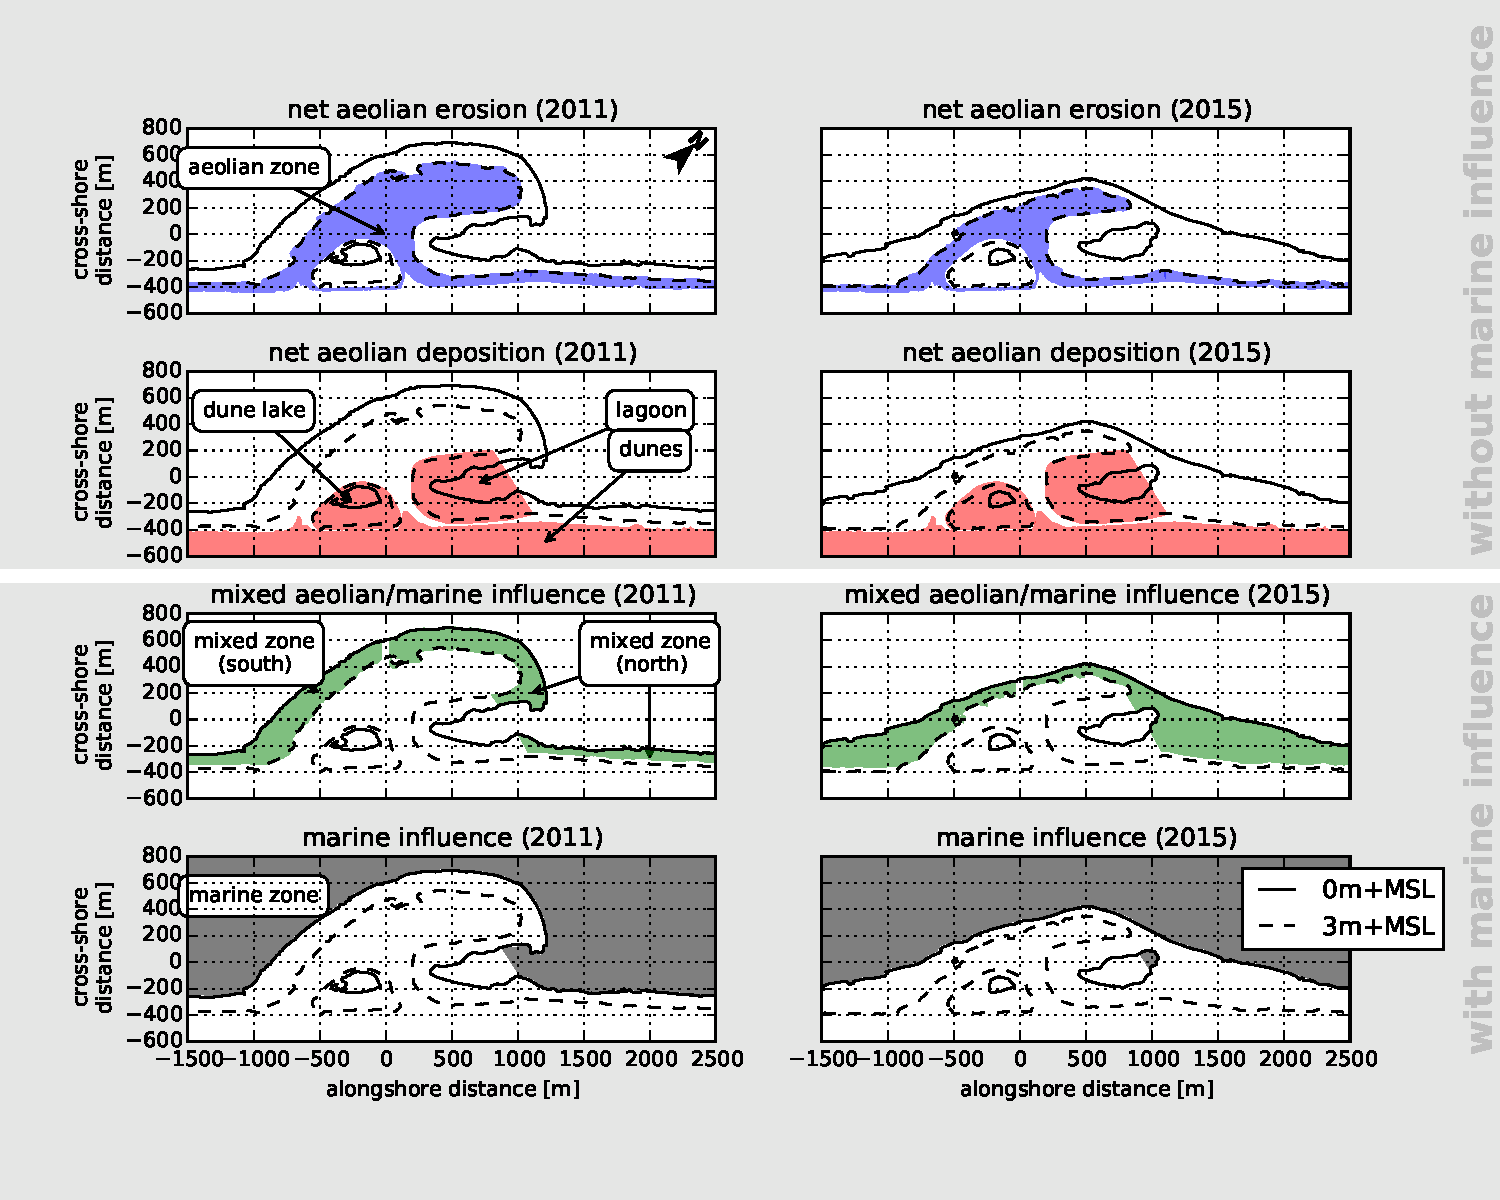
\includegraphics[width=\columnwidth]{../Figures/decomposition}
  \caption{Zonation of the Sand Motor domain into zones with net
    aeolian erosion and no marine influence, net aeolian deposition
    and no marine influence, mixed aeolian/marine influence and marine
    influence. Zonation is based on the 0, 3 and 5 m+MSL contour lines
    that roughly correspond with the mean water level, maximum runup
    level or berm edge and the dune foot respectively. Left panels:
    2011. Right panels: 2015. Source: \citet{Hoonhout2017a}.}
  \label{fig:decomposition2}
\end{figure}

The calibration is performed based on the bi-monthly erosion and
deposition volumes as measured in the Sand Motor domain
\citep{Hoonhout2017a}. The erosion and deposition volumes are
determined within seven predefined zones (Figure
\ref{fig:decomposition2}) that aim to separate areas with marine
influences from areas without marine influences, and separate areas
with net aeolian erosion from areas with net aeolian deposition. The
zonation is based on the 0, 3 and 5 m+MSL contour lines that roughly
correspond with the mean water level, maximum runup level or berm edge
and the dune foot respectively. The average $\mathrm{R^2}$ value of
the time series for erosion and deposition is used as benchmark. The
$\mathrm{R^2}$ value represents the fraction of explained variance and
is defined as:

\begin{equation}
  \label{eq:r2}
  R^2 = \frac{\sum_n \left[ V^n_{\mathrm{measured}} - V^n_{\mathrm{model}} \right]^2}{\sum_n \left[ V^n_{\mathrm{measured}} - \overline{V^n_{\mathrm{measured}}} \right]^2}
\end{equation}

\noindent where $V^n$ is the measured or modeled sediment volume in
time period $n$. The overbar denotes time-averaging. In addition the
root-mean-square error (RMSE) is presented as absolute measure for the
model accuracy, which is defined as:

\begin{equation}
  \label{eq:rmse}
  RMSE = \sqrt{\sum_n \left[ V^n_{\mathrm{measured}} - V^n_{\mathrm{model}} \right]^2}
\end{equation}

\noindent The calibration itself is performed in three steps:

\begin{enumerate}
\item A coarse calibration on $\sigma$ and $T_{\mathrm{dry}}$.
\item A calibration on $T$ using the provisional optimal settings for
  $\sigma$ and $T_{\mathrm{dry}}$.
\item A fine calibration on $\sigma$ and $T_{\mathrm{dry}}$ using the
  optimal setting for $T$.
\end{enumerate}

\section{Results}

The optimal model settings were chosen from 150 realizations (Figure
\ref{fig:calibration}). The optimal realization has an $\mathrm{R^2}$
value of 0.92 and a RMSE of $3 \cdot 10^4 ~ \mathrm{m^3}$.
\mrq{4.1} % (Table \ref{tab:stats}).
The corresponding optimal parameter settings are found to be
$\sigma = 9.2$, $T_{\mathrm{dry}} = 2$ h and $T$ = 1 s. These
settings were ultimately selected from a cluster of realizations with
comparable $\mathrm{R^2}$ values based on the relative sediment supply
from the mixed zones (Figure \ref{fig:decomposition2}, third row) at
the end of the simulation. An overview of all model settings for the
calibrated model is given in Appendix \ref{apx:modelsettings}.

%\begin{table}
%  \centering
%  \caption{Performance statistics of the calibrated Sand Motor model
%    for the calibration and test period.}
%  \label{tab:stats}
%  \begin{tabular}{lcccc}
%    Period & \multicolumn{2}{c}{RMSE} & $\mathrm{R}^2$ & rel. supply from \\
%    ~ & [$\mathrm{m^3}$] & [\%] & [-] & intertidal beach \\
%    \hline
%    2011 -- 2015 & $2.9 \cdot 10^4$ & 7.2 & 0.93 & 56\% \\
%    2015 -- 2016 & $2.9 \cdot 10^4$ & 7.2 & 0.93 & 56\% \\
%  \end{tabular}
%\end{table}

\begin{figure}
  \centering
  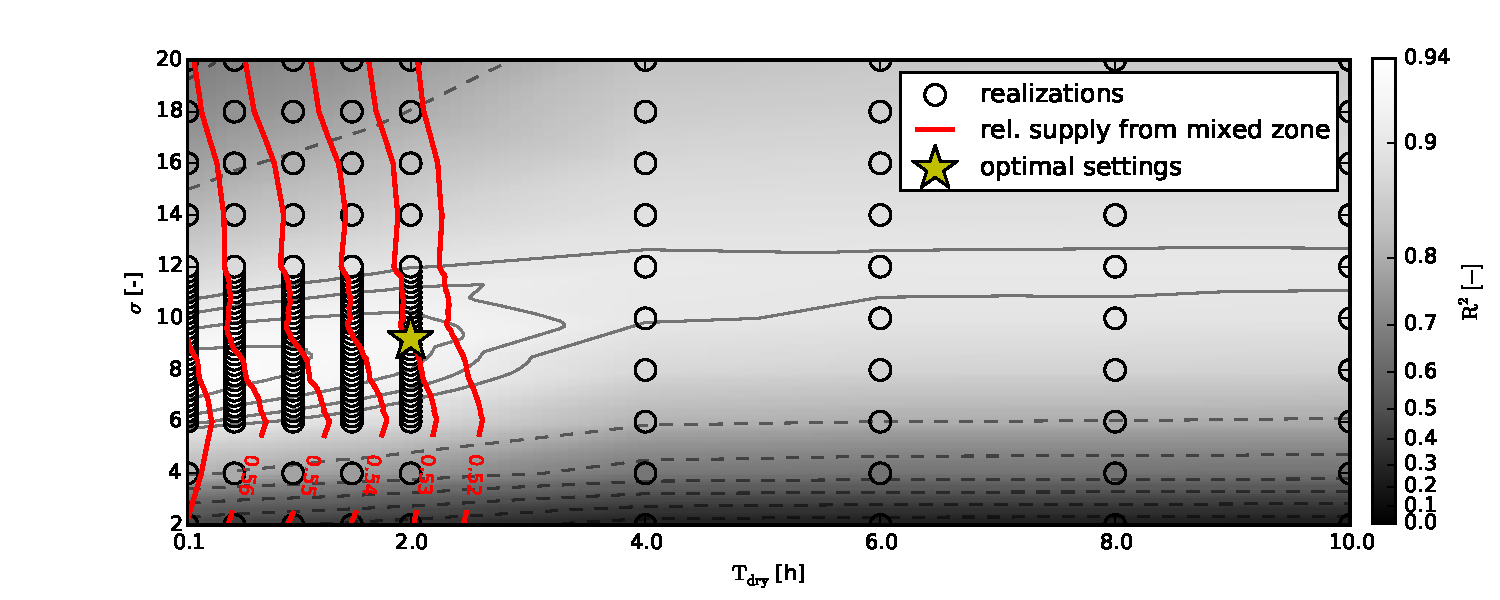
\includegraphics[width=\columnwidth]{../Figures/calibration}
  \caption{Systematic variation of calibration parameters $\sigma$ and
    $T_{\mathrm{dry}}$ with $T$ = 1 s. The circles indicate the
    realizations made. The colored background depicts a linear
    interpolation of the $\mathrm{R^2}$ values with respect to the
    data presented in Figure \ref{fig:netvolumechange}. The solid
    isolines depict $\mathrm{R}^2$ values from 0.90 to 0.93, while the
    dashed isolines depict $\mathrm{R}^2$ values from 0.0 to 0.9. The
    red lines depict the relative supply from the mixed zones ranging
    from 52\% to 57\%. The yellow star indicates the optimal value
    model settings.}
  \label{fig:calibration}
\end{figure}


\begin{figure}
  \centering
  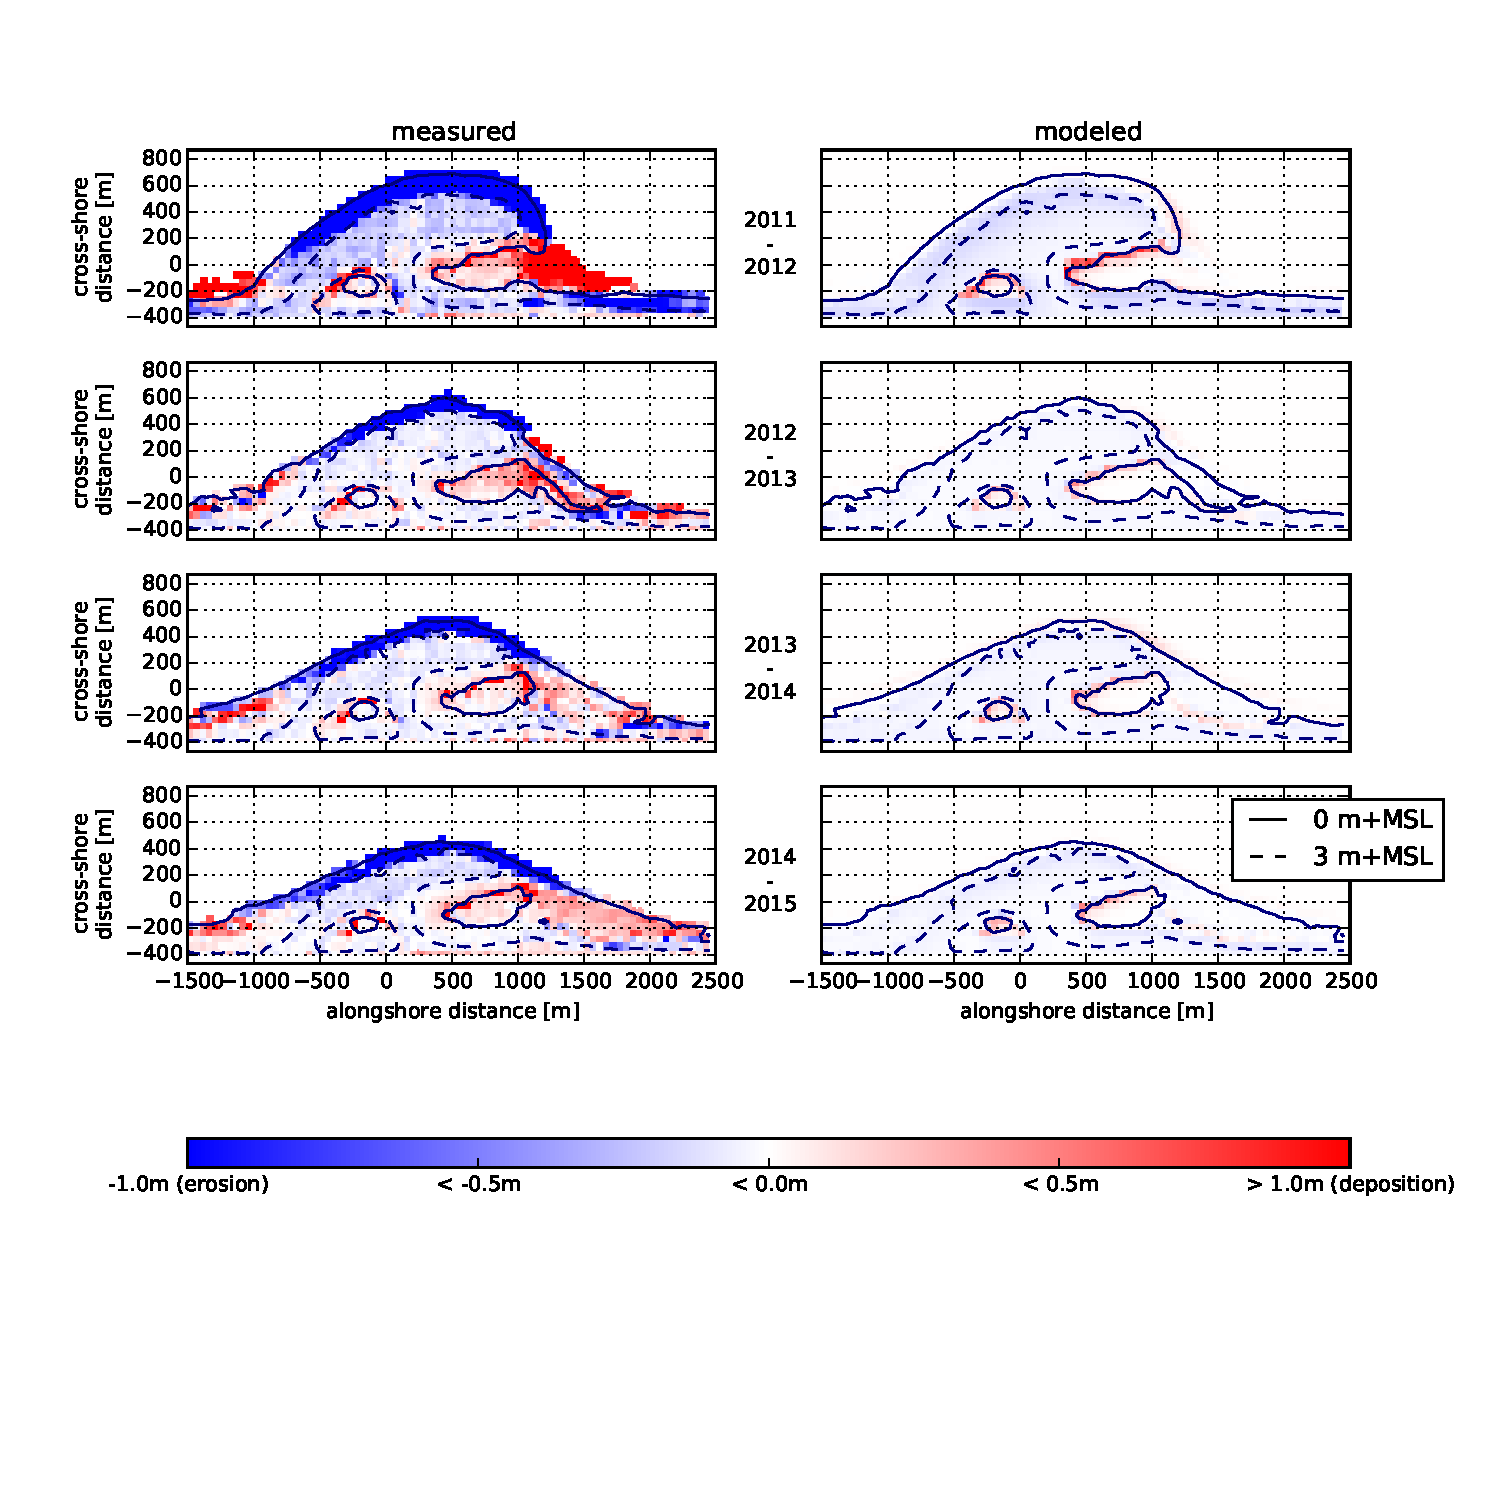
\includegraphics[width=\columnwidth]{../Figures/model_sedero}
  \caption{Measured and modeled yearly sedimentation and erosion
    above 0 m+MSL. Model results only include aeolian sediment
    transport as hydrodynamic sediment transport is not
    computed. Comparisons are made between the September surveys of
    each year.}
  \label{fig:sedero_model}
\end{figure}

\begin{figure}
  \centering
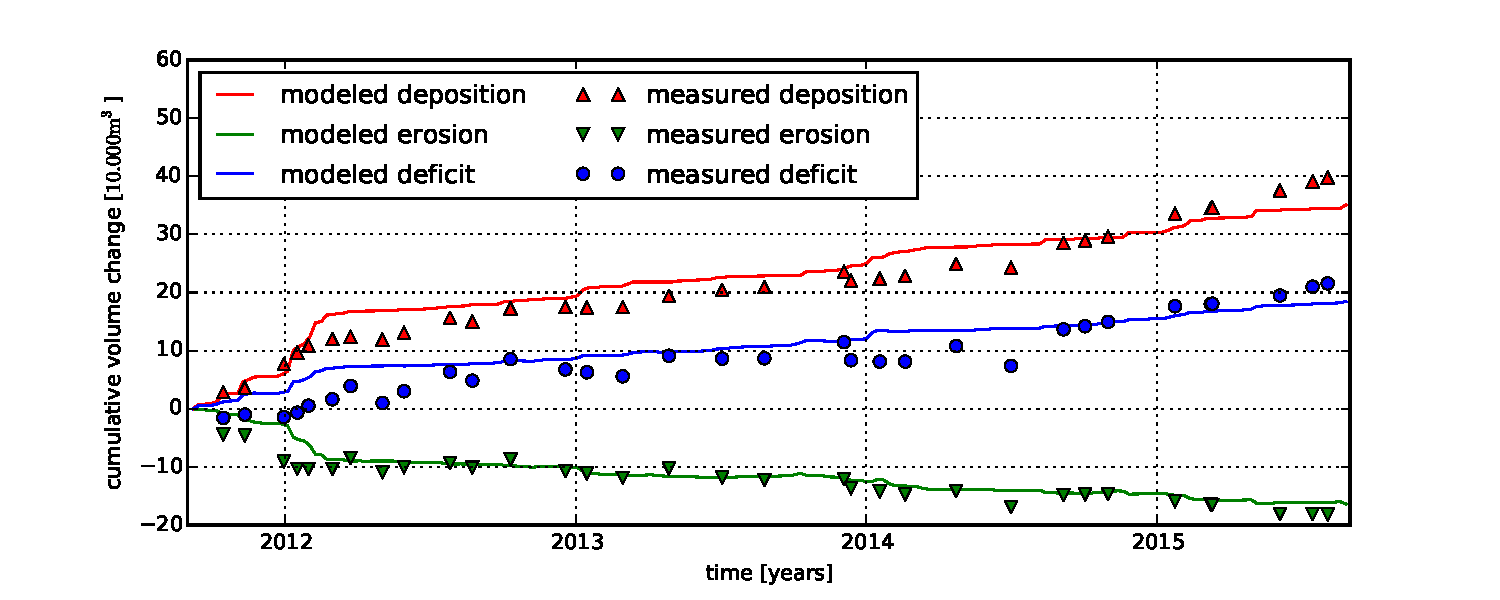
\includegraphics[width=\columnwidth]{../Figures/model_volumes_ts}
\caption{Measured and simulated net volume change of erosion and
  deposition volumes as presented in Figure
  \ref{fig:netvolumechange}.}
  \label{fig:netvolumechange_model}
\end{figure}

\begin{figure}
  \centering
  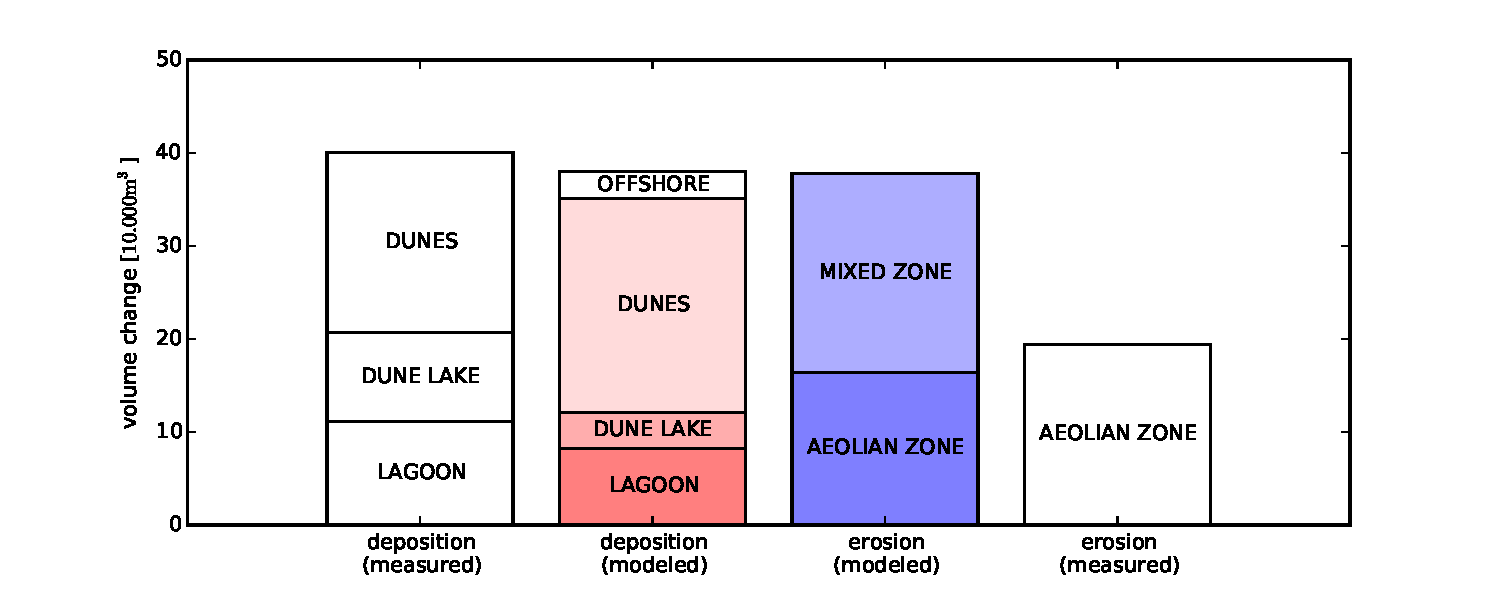
\includegraphics[width=\columnwidth]{../Figures/model_volumes}
  \caption{Total erosion and deposition volumes at the end of the
    simulation and measured total erosion and deposition volumes as
    presented in Figure \ref{fig:volumes_bars}.}
  \label{fig:volumes_bars_model}
\end{figure}

\begin{figure}
  \centering
  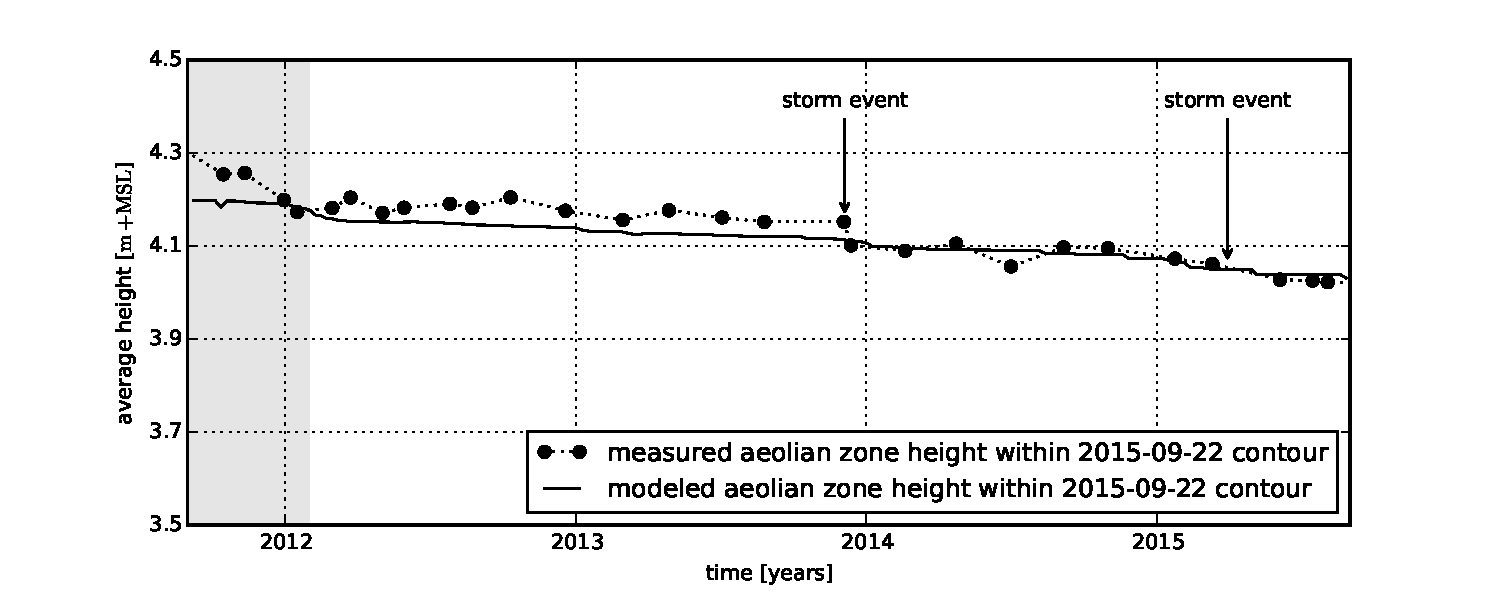
\includegraphics[width=\columnwidth]{../Figures/model_heights}
  \caption{Measured and simulated average beach height in the aeolian
    zone as presented in Figure \ref{fig:heights}.}
  \label{fig:heights_model}
\end{figure}

\begin{figure}
  \centering
  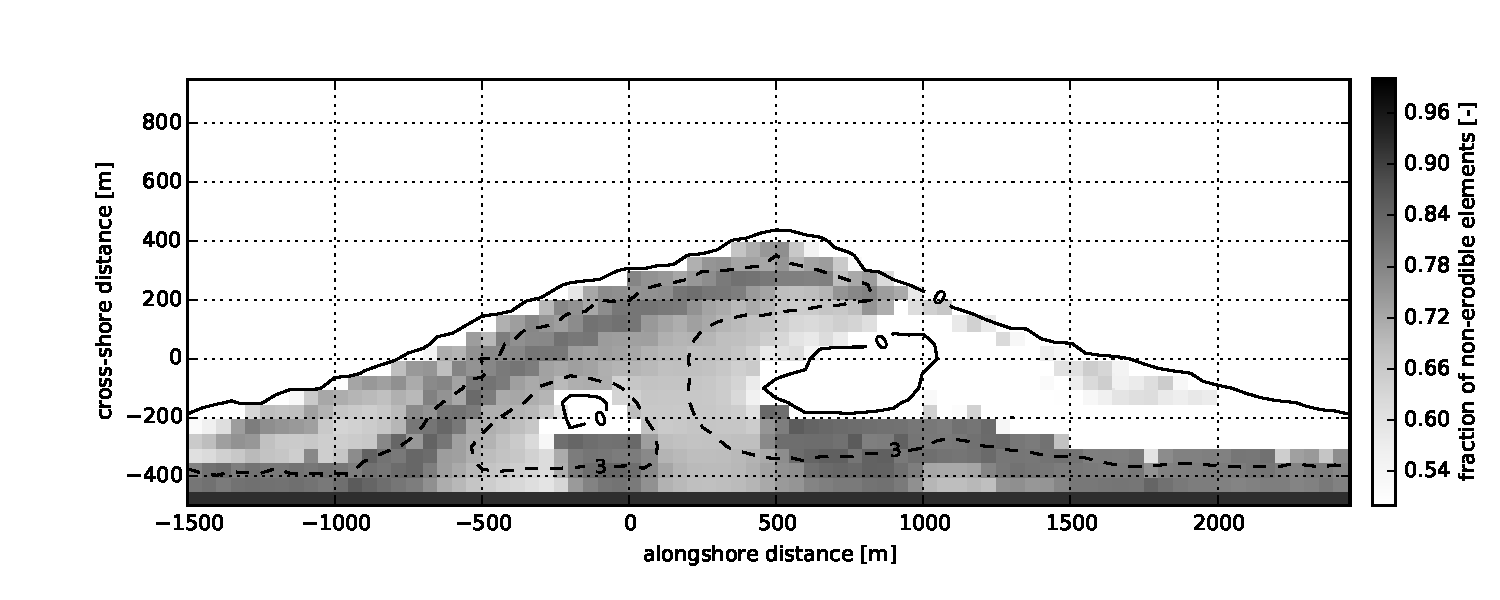
\includegraphics[width=\columnwidth]{../Figures/model_shellfraction}
  \caption{Simulated shell fraction in the aeolian zone at the end of
    the simulation.}
  \label{fig:shellfraction_model}
\end{figure}

Figure \ref{fig:sedero_model} shows that erosion from the aeolian zone
(Figure \ref{fig:decomposition2}, first row) is most pronounced in the
first year and least in the second year in both the measurements and
the model results. Also the deposition of aeolian sediment in the dune
lake and lagoon (Figure \ref{fig:decomposition2}, second row) is
observed in both the measurements and model results, although the
model underestimates these deposited volumes. The deposition in the
dune lake and lagoon is also more localized in the measurements than
in the model results. The spatial variability in the erosion of the
aeolian zone is larger in the measurements than in the model
results. The large variability measured in the mixed zone is not
present in the model results as hydrodynamic sediment transport is not
simulated.

The development of the total erosion and deposition volumes in the
Sand Motor domain in the four year period is represented well by the
model (Figure \ref{fig:netvolumechange_model}). The dune accumulation
volume is overestimated at the expense of the sediment volumes
deposited in the dune lake and lagoon (Figure
\ref{fig:volumes_bars_model}). As the dune area is not included in the
model domain, the sediment flux over the onshore boundary is assumed
to settle in the dunes entirely. The total sediment accumulation at
the end of the simulation is underestimated by 12\% as the offshore
sediment deposits are not included in the large scale sediment budget
analysis that are used for comparison. The underestimation is unique
for the last nine months of the simulation as the model overestimates
the total sediment accumulation with 5\% on average (Figure
\ref{fig:netvolumechange_model}). The relative importance of the mixed
zone as supplier of aeolian sediment is well captured. \mrq[hc]{1.3}

The change in beach height within the most recent 3 m+MSL contour,
that marks the aeolian zone, is represented by the model as the
$\mathrm{R^2}$ value is 0.71 and the RMSE is about 4 cm or 12\% of the
average bed level change (Figure \ref{fig:heights_model}). As the
change in beach height is computed within the most recent 3 m+MSL
contour, the discrepancy is illustrative for the differences in
spatial variability in erosion between measurements and model
results. The lowering of the beach in the aeolian zone in the first
half year of the simulation is particularly underestimated, while the
accelerated erosion in this period is well captured in the total
sediment transport. This indicates that sediment is eroded from
outside the most recent 3 m+MSL contour.

The coverage of non-erodible elements $\sigma \lambda$ [-] (Equation
\ref{eq:roughness_density}) in the aeolian zone varies between 60\%
and 80\% at the end of the simulation (Figure
\ref{fig:shellfraction_model}). The coverage is high compared to the
10\% -- 20\% shell coverage estimated to be present at the Sand Motor
above 3 m+MSL based on gridded photographs.
% (Figure \ref{fig:armoring}).

\begin{figure}
  \centering
  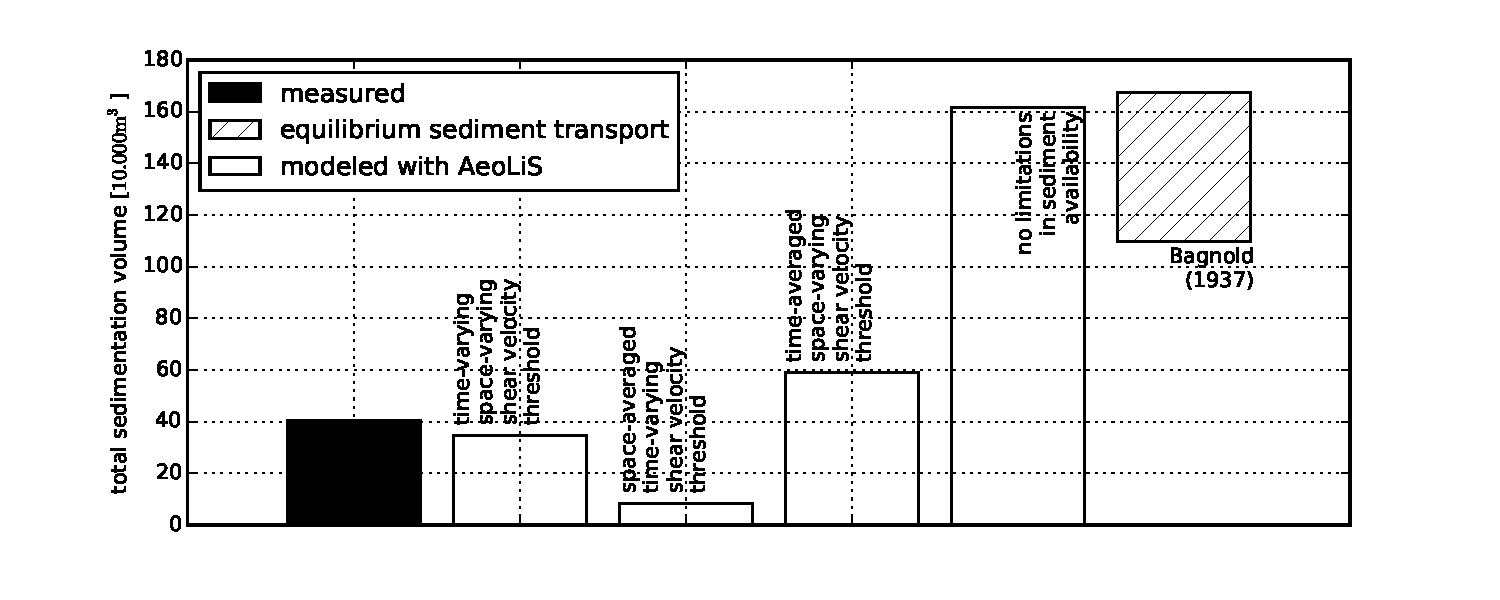
\includegraphics[width=\columnwidth]{../Figures/space_vs_time}
  \caption{The influence of time-varying and space-varying shear
    velocity thresholds on the total sedimentation volume. The two
    leftmost bars depict the measured and modeled sedimentation volume
    as obtained from the calibrated model (Figure
    \ref{fig:volumes_bars_model}). The middle two bars depict results
    from two separate model simulations in which a space-averaged
    threshold time series or a time-averaged threshold field is
    imposed respectively. The threshold averages are based on the
    result from the calibrated model. The two rightmost columns depict
    a result from a separate model simulation with a constant uniform
    threshold based on only a constant uniform median grain size and
    the estimated equilibrium sediment transport following
    \citet{Bagnold1937a} respectively (Table \ref{tab:models}).}
  \label{fig:space_vs_time}
\end{figure}

Both the spatial and temporal variations in aeolian sediment
availability are crucial for an accurate description of total
sedimentation and erosion volumes as well as an accurate prediction of
the aeolian sediment source and deposition areas. \mrq[hc]{4.3} Figure
\ref{fig:space_vs_time} compares the total sedimentation volume
according to measurements, the calibrated model and additional
simulations, that are variations of the calibrated model in which
spatial and/or temporal variations in the shear velocity threshold are
averaged out. During these additional simulations the shear velocity
threshold is not computed by the model, but space- and/or
time-averaged thresholds based on the model results of the calibrated
model are imposed. Negligence of the spatial variations results in a
79\% underestimation of the total sedimentation volume and a relative
contribution of 8\% of the mixed zones. The negligence of the temporal
variations results in a 46\% overestimation of the total sedimentation
volume and a relative contribution of 86\% of the mixed zones.  In
addition, a simulation without limitations in sediment availability
overestimates the measured total sedimentation volumes with 400\%,
which is comparable to the wind transport capacity following
\citet[][Figure \ref{fig:models}]{Bagnold1937a}.

% R^2

% distribution between areas

% beach height

% shell coverage

% runup not taken into account

%\begin{figure}
%  \centering
%\includegraphics[width=\columnwidth]{../Figures/volumes_ts_forecast}
%\caption{Measured and simulated net volume change of erosion and
%  deposition volumes for the period September 1, 2015 to September 1,
%  2016 that was not included in the model calibration.}
%  \label{fig:netvolumechange_model2}
%\end{figure}
%
%The comparison of measurements and model results for the period
% between September 1, 2011 and September 1, 2015 illustrates the
% descriptive capabilities of the model. Figure
% \ref{fig:netvolumechange_model2} shows the measured and modeled
% volume change between September 1, 2015 and September 1, 2016. The
% continuation of the total sediment accumulation is predicted [TODO],
% given the $\mathrm{R^2}$ of [TODO] and RMSE of
% [TODO]\%.

\section{Discussion}

The model results show that multi-annual aeolian sediment erosion and
deposition volumes, and the relative importance of the mixed zones as
source of aeolian sediment are reproduced with reasonable
accuracy. This suggests that indeed significant limitations in
sediment availability, due to soil moisture content and beach
armoring, govern aeolian sediment transport in the Sand Motor domain.
A comparison with a simulation without limitation in sediment
availability suggests that aeolian sediment availability in the Sand
Motor domain is limited to about 25\% -- 35\% of the wind transport
capacity.

The negligence of spatial variations causes the model to underestimate
the measured total sedimentation volume. The sediment supply from the
relatively small mixed zone is marginalized as the imposed
space-averaged shear velocity threshold is relatively high. In
contrast, the negligence of temporal variations causes the model to
overestimate the measured total sedimentation volume. The sediment
supply from the mixed zones is increased as the effect of its periodic
flooding is averaged out. At the same time, the sediment supply from
the aeolian zone is decreased as the influence of beach armoring
affects sediment availability from the start of the simulation rather
than after the development of the beach armor layer. Therefore, the
total sedimentation volume is not only overestimated, but also the
importance of the mixed zones as supplier of aeolian sediment.

\subsection{Seasonal and local variations in sedimentation and
  erosion}

% advection assumption / diffusion / gusts
%The advection equation in combination with a diffusive numerical
%scheme results in smooth solutions. Small-scale variability in erosion
%and deposition are therefore not described by the model. Besides,
%measured local variations are likely promoted by local variations in
%initial topography and bed composition that also induce local
%variations in wind shear. These initial variations are not taken into
%account in the simulations.

The model can reproduce multi-annual trends in sedimentation volume,
which is the aim of the hindcast, but seasonal and local variations
are sometimes not represented by the model. An analysis of these
variations is interesting as they influence the accuracy of specific
model results.

Average wind speeds tend to be elevated in December and January
(Figure \ref{fig:boundaryconditions}), which leads to short periods of
accelerated sediment accumulation in the beginning of 2012, 2013 and
2015 that are captured well by the model. Early 2014 no accelerated
sediment accumulation is measured, while the model simulation shows an
increase in sediment accumulation originating from the mixed zones
similar to other years.

The discrepancy early 2014 might be explained by topographic changes
induced by hydrodynamic forces. On December 5th, 2013 an exceptional
storm hit the Dutch coast. During this storm a significant decrease in
aeolian deposits in the lagoon was observed, while deposits in the
dunes and dune lake increased only marginally. The assumption that the
closed end of the lagoon is mainly governed by aeolian sediment
transport might be violated in these exceptional conditions. At the
same time, the erosion of the aeolian zone that day equaled the total
erosion of the aeolian zone that year. Consequently, the total
subaerial sediment volume decreased that day with about
$\mathrm{1 \cdot 10^4}$ $\mathrm{m^3}$, possibly caused by
hydrodynamic forces. This suggests that the simplified hydrodynamics,
despite the use of a hydrodynamic mask, are a limiting factor in
describing the Sand Motor's subaerial morphodynamics during extreme
storms.

In the first months of the simulation, the total sediment accumulation
is well represented, but erosion of the aeolian zone is
underestimated. As beach armoring is the most important availability
limitation in the aeolian zone, this suggests that the armoring rate
is overestimated by the model. The armoring rate is mainly influenced
by initial shell fraction of 5\%, which might be
overestimated. Alternatively, the initially uniform distribution of
shells in the bed is not an accurate representation of reality.

Measured erosion and deposition rates exceed modeled erosion and
deposition rates in the final nine months of the simulation. In this
period dune growth seems to accelerate, while neither the deposition
in the dune lake and lagoon did accelerate nor did the wind speed
increase. The apparent acceleration is therefore solely found in the
half yearly lidar measurements of the dune area \citep{Hoonhout2017a}
and is consequently based on a single data point. Despite the
uncertainty involved in the measured acceleration, also precipitation
rates, that were up to 70\% lower in this period compared to the same
period in other years, might explain the discrepancy at the end of the
simulation \citep{Jackson1998}. For the hindcast no precipitation time
series are imposed as the effect on the aeolian sediment transport
rate is not properly understood yet. Consequently, the calibration of
the model might have resulted in an overestimated importance of beach
armoring to compensate for the negligence of precipitation.

% morphological feedback
The distribution of the aeolian sediment deposits over the dune lake,
lagoon and dunes is not represented well as deposits in the dune lake
and lagoon are underestimated. Additional hydrodynamic and hydrologic
processes, like wind setup and groundwater seepage, might cause the
entrapment area in reality to be larger than modeled. But more
importantly, the dune lake and lagoon are positioned in the lee of the
Sand Motor crest with respect to the predominant southwesterly wind
direction. The height difference between the Sand Motor crest and the
water level in the lagoon and dune lake is several meters, which is
likely to influence the local wind field significantly. The probable
decrease in wind shear in the lee of the Sand Motor crest promotes
deposition of aeolian sediment and likely hampers supply to the
dunes. These local variations in wind shear are not included in the
simulations.

\subsection{Beach armoring, sediment availability and the shear
  velocity threshold}

% As the $\sigma$ value is an optimal average for the entire model
% domain and duration it can be questioned if an incidental increase
% in soil moisture due to precipitation can influence sediment supply
% significantly.

\begin{figure}
  \centering
\includegraphics[width=\columnwidth]{../Figures/sigma}
\caption{Relation between shear velocity threshold, shell coverage and
  $\sigma$ according to \citet[][Equation
  \ref{eq:raupach2}]{Raupach1993}. The shaded areas indicate the
  relevant parameter ranges from \citet{McKennaNeuman2012} (blue) and
  the model results (green).}
  \label{fig:sigma}
\end{figure}

The influence of beach armoring is reflected in the model by both
$\sigma$ and the roughness density $\lambda$ (Equation
\ref{eq:raupach2} and \ref{eq:roughness_density}). The optimal value
for $\sigma$ was found to be 9.2, which is high compared to the value
of 4.2 found by \citet{McKennaNeuman2012}. The difference suggests
that the roughness elements at the Sand Motor protrude less from the
bed compared to what was found in the wind tunnel
experiments. Consequently, the importance of beach armoring would be
relatively low at the Sand Motor. However, the low $\sigma$ value is
largely compensated by the roughness density $\lambda$ reflected in a
shell coverage $\sigma \lambda$ that is high compared to what was
found in the wind tunnel experiments (12\% -- 43\% on average) and
what is found at the Sand Motor field site (10\% -- 20\%). Figure
\ref{fig:sigma} shows that the combination of high shell coverage and
$\sigma$ value results in a very similar increase of the shear
velocity threshold compared to the wind tunnel experiments presented
by \citet{McKennaNeuman2012}.

The reason that the model calibration resulted in this particular
value for $\sigma$ is that the model does not differentiate between
the fluid and impact velocity threshold.  Therefore, the roughness
elements in the model affect the initiation of sediment transport
equal to the continuation of sediment transport. The potential
reduction in sediment availability increases with a decreasing value
for $\sigma$ (if $m$ = 0.5, Figure \ref{fig:sigma}) and is implemented
through an increase in shear velocity threshold. The shear velocity
threshold also affects aeolian sediment already in transport and
originating from upwind, unarmored beach areas, like the mixed
zones. Sediments from upwind areas are therefore partially deposited
in the aeolian zone as soon a beach armor layer develops. For low
values for $\sigma$ the local deposition of sediment from upwind areas
is already significant with low shell coverage. Low $\sigma$ values
therefore reduce the total sediment accumulation in the dunes
quickly. In order for the model to provide reasonable total sediment
transport rates, a higher value for $\sigma$ was found in the
calibration that ultimately induces a higher shell coverage. The value
for $\sigma$ therefore does not only represent a spatiotemporal
averaged emergence of roughness elements, but also a compromise
between its effect on the fluid and impact velocity threshold.
%The
%implementation of roughness elements in the model can explain the high
%value for $\sigma$, but it particularly illustrates the necessity to
%differentiate between initiation and continuation.% of motion as
%observed in recent laboratory measurements (REFS RALEIGH MARTIN).
% associated with the fluid and impact velocity threshold respectively.

%\subsection{Predictive capabilities of the model}
%
%The period from September 1, 2015 to September 1, 2016 was not
% included in the calibration. Simulation of the total sediment
% accumulation in this period therefore provides insight in the
% predictive capabilities of the calibrated model. The
% $\mathrm{R}^2$ and RMSE values suggests that the model
% has both descriptive and predictive capabilities.




% average wind vs gusts

% wind field

% bed composition layers

% offshore deposits

% salt crusts

% distinction between thresholds for entrainment and continuation

\section{Conclusions}

The Sand Motor hindcast shows that the reduction of aeolian sediment
availability due to soil moisture and beach armoring can largely
explain the low accumulation volumes in the Sand Motor domain. The
\textsc{AeoLiS} model has shown to be quantitatively valuable and
practically applicable. The model provides a framework for the
description of complex spatiotemporal variations in aeolian sediment
availability and its relation to sediment transport that has not yet
been exploited in full.

\bigskip

\noindent From the hindcast the following conclusions can be drawn:

\begin{itemize}
\item The \textsc{AeoLiS} model is able to reproduce multi-annual
  aeolian sediment transport rates in the Sand Motor domain in the
  four years after its construction with a RMSE of
  $3 \cdot 10^4 ~ \mathrm{m^3}$ and $\mathrm{R^2}$ of 0.92 when time
  series of measured and modeled total aeolian sediment transport
  volumes are compared.
\item The \textsc{AeoLiS} model is able to reproduce large scale
  spatial patterns in aeolian sediment transport in the Sand Motor
  domain in the four years after its construction, but underestimates
  the deposition in the dune lake and lagoon.
\item The \textsc{AeoLiS} model overestimates the total sedimentation
  volume with 5\% on average, but underestimates the total
  sedimentation volume with 12\% at the end of the simulation. The
  discrepancy at the end of the simulation might be caused by a
  particularly dry season as precipitation is not included in the
  simulations.
  % \item The \textsc{AeoLiS} model has predictive capabilities as the
  %   calibrated model describes new period of measurements with a
  %   RMSE of XX\% and $\mathrm{R}^2$ of 0.XX.
\item The \textsc{AeoLiS} model is able to capture the seasonal
  variations in sediment transport in all years, except for early 2014
  when significant morphological change is possibly related to
  hydrodynamic sediment transport that is not included in the
  simulations.
\item The \textsc{AeoLiS} model overestimates the shell coverage,
  which compensates the high value for $\sigma$. The high $\sigma$
  value is a compromise between the fluid and impact threshold that
  are currently assumed to be equal.
\item The combination of spatial and temporal variations in aeolian
  sediment availability, due to the combined influence of soil
  moisture, sediment sorting and beach armoring, and the feedback
  between aeolian sediment availability and transport is essential for
  an accurate estimate of the total sedimentation volume and the
  corresponding aeolian sediment source areas in the Sand Motor
  domain.
\end{itemize}

%%% Local Variables:
%%% mode: latex
%%% TeX-master: "thesis"
%%% End:


\cleardoublepage
\part{Discussion and conclusions}

\chapter{Discussion} \label{ch:discussion}

This thesis explored the nature of aeolian sediment availability.
Aeolian sediment availability is generally associated with the shear
velocity threshold. Alternatively, sediment availability can be
expressed in terms of critical fetch \citep{Bauer2002} or explicitly
following \citet{deVries2014b}. The latter two approaches deviate
rather radically from the legacy of aeolian research. Both discard the
abundantly available relations between bed surface properties,
sediment availability and the shear velocity threshold. Instead, they
describe sediment availability in new terms for which no
quantification is known. In Chapter \ref{ch:model} it is argued that
the new approaches have a right to exist as they allow for an
increased complexity in situations that can be described by
models. Ultimately, the approach of \citet{deVries2014b} is adopted
for this thesis and adapted to support multi-fraction sediment
transport in order to simulate sediment sorting and beach armoring
that introduces feedback between aeolian sediment availability and
transport in aeolian sediment transport modeling.

The model approach presented in this thesis is a unification of the
classic approach based on the shear velocity threshold and the
approach of \citet{deVries2014b}. Whereas \citet{deVries2014b} use a
user-defined value for the sediment availability $m_{\mathrm{a}}$ (or
$S_{\mathrm{e}}$) to truncate the instantaneous sediment transport in
their model, the approach presented in this thesis uses simulation to
determine the local sediment availability $m_{\mathrm{a,k}}$. The
weighting factor $\hat{w}_k$ is subsequently adapted to the local
sediment availability (Equation \ref{eq:erodep_multi}). Since the
weighting factor $\hat{w}_k$ is essentially a space- and
time-dependent modification to the shear velocity threshold, this new
approach connects the field of availability-limited aeolian sediment
transport modeling with the long history of aeolian
research. \mrq[d]{3.2}

Availability-limited aeolian sediment transport modeling can be
further improved by distinguishing between the fluid and impact
threshold in future versions of the presented model. The presented
model provides a framework in which such distinction can be made
rather naturally. The bed interaction parameter essentially implements
this distinction already for armored beach surfaces, but a more
generic implementation is required for coastal systems with large
spatial variations in sediment availability. A key issue is still that
relations between bed surface properties, sediment availability and
the shear velocity threshold are typically derived as bulk formulation
for the fluid and impact threshold together. A proper implementation
of the fluid and impact threshold in the presented model therefore
depends on a substantial investment in data collection
\citep{Martin2016}.

The presented model for availability-limited aeolian sediment
transport can also be applied to availability-abundant coastal
systems. However, much of the complexity in coastal aeolian sediment
transport modeling is related to aeolian sediment availability. The
approach might be considered too complex for more regular situations
where sediment availability is abundant. A key issue is that assessing
whether a coastal environment is availability-limited or not, is not
trivial. In this thesis established formulations for equilibrium
aeolian sediment transport are used to roughly estimate the sediment
availability of coastal systems. However, if the presented model is
proven to be sufficiently accurate in availability-abundant coastal
systems, it might be used to formulate rules of thumb to assess
coastal systems on their sediment availability more
accurately. Subsequently, the model might be used to assess these
coastal systems that are found to be availability-limited or
facilitate the formulation of aggregated relations between aeolian
sediment availability and transport that would serve a more rapid
assessment.

In hindsight, the chapters in this thesis reveal a certain chronology
in understanding the phenomenon of aeolian sediment availability.
Deducing the significance of sediment availability from the large
scale sediment budget analysis or the small scale sediment transport
measurements was not trivial as sediment availability appeared to be
rather intangible. This started with the slightly ambiguous use of
terminology in literature where, for example, \emph{sediment supply}
is often mistaken to be equal to \emph{sediment availability} or the
\emph{shear velocity threshold}. In addition, various aeolian, marine
and meteorological processes affect aeolian sediment availability
and/or the shear velocity threshold differently and on various
temporal and spatial scales. Consequently, significant time was spent
to narrow down the essence of sediment availability and define a
distinctive terminology accordingly. The phenomenon of aeolian
sediment availability was made tangible in a numerical model for
aeolian sediment availability and transport that is unique in that it
describes aspects essential to aeolian sediment availability and
transport modeling that have previously been subject to research, but
never been combined in a comprehensive model approach. The main
contribution of the model is the \emph{combined} simulation of:

\begin{enumerate}
\item Temporal variations in aeolian sediment availability and
  transport.
\item Spatial variations in aeolian sediment availability and
  transport.
\item Recurrence relation between aeolian sediment availability and
  transport through self-grading of sediment.
\item Simulation of multiple availability-limiting processes and their
  combined influence on aeolian sediment transport.
\item Natural differentiation between fluid and impact shear velocity
  threshold (not implemented).
\end{enumerate}

%\section{Future model improvements}

As illustrated by the Sand Motor hindcast presented in Chapter
\ref{ch:hindcast}, the combined influence of various aspects of
aeolian sediment availability is essential to obtain reliable
estimates of aeolian sediment transport and dune growth for which the
presented model provides a general framework. Notwithstanding that
model development just started and needs further extension,
calibration and validation to make it generally applicable.

Based on the Sand Motor hindcast several opportunities for future
model improvement have been identified:

\begin{itemize}
\item Support for local variations in wind shear due to morphological
  feedback.

  Neither deposition in front of the dunes nor deposition in the lee
  of the Sand Motor crest is currently simulated as morphological
  feedback with the wind is not taken into account. Given the
  discrepancy in the spatial distribution of aeolian sediment deposits
  between measurements and model result, it seems advisable to provide
  the model with local variations in wind shear. The model of
  \cite{Kroy2002} based on the derivation of the local wind field by
  \citet{Weng1991} might provide a description of the local variations
  in wind shear for which the computational effort relates well to the
  presented model.

%\item Support for local variations in wind shear due to the presence
%  of vegetation.
%
%  No deposition in the dunes is currently simulated as the reduction
%  in wind shear due to the presence of vegetation is not taken into
%  account. The model of \citet{Duran2013} as an extension to the model
%  of \citet{Kroy2002} might provide this functionality.

\item Support for the effect of wind gusts.

  The calibrated model is forced by an hourly averaged wind time
  series. The use of hourly averaged values for wind speed neglects
  the gustiness of the wind. Wind gusts might influence sediment
  transport significantly as the relation between wind speed and
  sediment transport is nonlinear. However, providing the model with
  high resolution wind time series would require a less diffusive
  numerical scheme that would likely not be computationally feasible
  for long-term simulations. Moreover, since saltation is not purely
  an advective mode of transport, the assumption of advection might be
  violated for very short time scales as interaction with the bed
  becomes dominant.

  As an alternative, the influence of gusts can be parameterized. It
  can be argued that some persistence is needed for gusts to influence
  sediment transport, resulting in a lower boundary of the temporal
  resolution of the wind time series. The distribution of the wind
  speed with respect to the hourly average can then provide a basis
  for a gustiness factor that increases the global wind shear.

\item Support for differentiation between the fluid and impact shear
  velocity thresholds.

  The sediment transport capacity is currently implemented identical
  for the initiation and continuation of motion as no distinction
  between the fluid and impact threshold is made. The Sand Motor
  hindcast illustrates how this restriction affects the influence of
  roughness elements on aeolian sediment availability. Similar to the
  implementation of the bed interaction parameter, that distinguishes
  between the grain size distribution in the bed and the air, a
  distinction between fluid and impact threshold can be implemented.

  The right-hand side of the advection equation (Equation
  \ref{eq:erodep_multi}) can be modified according to:

  \begin{equation}
    \label{eq:erodep_split}
    E_k - D_k = \min \left( 
      \frac{\partial m_{\mathrm{a},k}}{\partial t} \quad ; \quad 
      \frac{\hat{w}_k}{T} \cdot \left[
        (1 - S_k) \cdot c^{\mathrm{fluid}}_{\mathrm{sat},k} +
        S_k \cdot c^{\mathrm{impact}}_{\mathrm{sat},k} - c_k
      \right]
    \right)
  \end{equation}

  \noindent where $c^{\mathrm{fluid}}_{\mathrm{sat},k}$
  [$\mathrm{kg/m^2}$] and $c^{\mathrm{fluid}}_{\mathrm{sat},k}$
  [$\mathrm{kg/m^2}$] are the sediment transport capacity associated
  with the fluid and impact threshold respectively and $S_k$ [-] is
  the degree of saturation defined as:

  \begin{equation}
    S_k = \sum_{k=1}^{n_{\mathrm{k}}} \frac{c_k}{c^{\mathrm{impact}}_{\mathrm{sat},k}}
  \end{equation}

  \noindent Note that the weighting factor $\hat{w}_k$ already
  distinguishes between sediment in the air and in the bed, depending
  on the saturation and the bed interaction parameter and therefore
  appears outside the brackets.

  Although the presented model conceptually allows to differentiate
  between the impact and fluid threshold, empirical data to quantify
  the differentiation is lacking. This model improvement is therefore
  hypothetical at the current stage of development.

\item Support for independent definition of the active bed layer.

  The top bed composition layer currently acts as active bed layer,
  but at the same time defines the vertical resolution of the sorting
  and armoring processes. As these are two fundamentally different
  properties of the model, it is advisable to define the active bed
  layer separate from the numerical resolution. A probability
  distribution can be defined that describes the probability of
  sediment to be eroded from a specific layer, which would logically
  decrease with the depth. The bed composition layer thickness would
  than uniquely determine the vertical resolution of sorting and
  armoring.

\item Use of online coupling with other models

  The Sand Motor hindcast showed the importance of an accurate
  description of the hydrodynamics for accurate estimates of the
  development of the aeolian sedimentation and erosion
  volumes. Similarly, groundwater seepage might influence the aeolian
  sediment deposition around the lagoon and dune lake, which would
  require a description of the groundwater level to be implemented.

  It can be questioned if such detailed descriptions of hydrodynamic
  and hydrological processes are still within the scope of an aeolian
  sediment transport model. Alternatively, online model coupling with
  dedicated models for near-shore hydrodynamics and hydrology can be
  pursued. A Basic Model Interface (BMI) was implemented to
  accommodate model coupling.

\end{itemize}

The Sand Motor appeared to be a valuable field site for investigating
the influence of aeolian sediment availability on long-term aeolian
sediment transport. The construction height, dry surface area and
considerable beach armoring and compartmentalization amplify the
processes governing aeolian sediment availability. These
characteristics make the Sand Motor also a peculiar coastal site that
might be better described as ``coastal desert'' than ``mega
nourishment''. The relative importance of processes governing aeolian
sediment availability are likely to be different at a more ordinary
coastal site. For example, beach armoring will not be as important on
narrow beaches that are frequently flooded. Preliminary model results
for more ordinary coastal sites suggest that the extent of the
compartmentalization of the beach is less, but spatiotemporal
variations in aeolian sediment availability can still have a
significant influence on aeolian sediment transport. A comparison
between field measurements from more ordinary coastal sites and model
results can provide insight in the relative importance of these
processes in general.

%Aeolian sediment availability is generally associated with the shear
%velocity threshold. Based on the subaerial evolution of the Sand Motor
%mega nourishment it is illustrated that practical application of the
%shear velocity threshold to describe the local aeolian sediment
%availability is not trivial. The shear velocity threshold is used to
%describe both the change in sediment transport capacity, associated
%with the impact threshold, as well as the change in sediment
%availability, associated with the fluid threshold. Moreover, the shear
%velocity is influenced by spatiotemporal variations in bed surface
%properties and the feedback between sediment transport and sediment
%availability, that require a process-based description of the shear
%velocity threshold.
%
%In Chapter \ref{ch:model} different approaches 
%
%
%the only existing model
%approach that could potentially fulfill these requirements is the
%availability-limited advection scheme following
%\citet{deVries2014b}. This approach is extended with a process-based
%description of soil moisture and sediment sorting and beach
%armoring. What is not obvious from the model description in Chapter
%\ref{ch:model} is that this approach appears to be equivalent to the
%traditional approach based on the shear velocity threshold. However,
%the shear velocity threshold is captured in an advection framework
%that allows for feedback with between sediment availability and
%transport as well as differentiation between the fluid and impact
%threshold.





% and
%reflects a certain chronology in understanding the phenomenon.  In
%Chapter \ref{ch:largescale} sediment availability is discussed in
%terms of potential and actual sedimentation volumes at the Sand Motor
%mega nourishment. The difference is generally associated with aeolian
%sediment availability and expressed in a shear velocity
%threshold. Alternatively, sediment availability can be expressed in
%terms of critical fetch \citep{Bauer2002} or explicitly following
%\citet{deVries2014b}. In Chapter \ref{ch:model} it is argued that
%these approaches are related, but differ in the complexity of
%situations they can describe. The approach of \citet{deVries2014b} is
%adopted and extended with a process-based description of soil moisture
%and sediment sorting and beach armoring. In Chapter \ref{ch:hindcat}
%this new approach is applied to the Sand Motor mega nourishment, which suggests that...




%Observations at the Sand Motor mega nourishment
%inspired the development of a numerical model that focuses on the
%quantification of aeolian sediment availability. Therefore the
%\textsc{AeoLiS} model should, in its current stage, be seen as a
%sediment availability rather than a sediment transport model.
%
%Past research on aeolian sediment availability focused mainly on the
%use of shear velocity thresholds. 

% the nature of limitations in sediment availability, the paradox, the connections


% time and space variability introduced, but initiation and conitunation distinction still to do

% ultimately: simple model








% average wind vs gusts


% bed composition layers


% winter vs. summer fluxes

% offshore fluxes

% alongshore variability

% salt crusts and other supply limiters

%%% Local Variables:
%%% mode: latex
%%% TeX-master: "thesis"
%%% End:


\chapter{Conclusions} \label{ch:conclusions}

This thesis concludes with addressing the research questions
formulated in the introductory chapter (Chapter
\ref{ch:introduction}). Each question is addressed with relevant
references to the four main chapters \ref{ch:largescale} to
\ref{ch:hindcast}.

\begin{description}
\item[Research objective \#1] Identify the main sources for aeolian
  sediment in coastal environments and particularly at the Sand Motor
  mega nourishment.

  \medskip

  The research questions and answers related to objective \#1 are:

  \begin{enumerate}[{1.}1]
  \item What is the total aeolian sediment supply at the Sand Motor
    mega nourishment?

    The total aeolian sediment supply accumulated to 400.000
    $\mathrm{m^3}$ in the first four years after construction of the
    Sand Motor\rrq{1.2ls}. About 120.000 $\mathrm{m^3}$ accumulated in
    the first half year after construction. From January 2012 the
    accumulation rate of aeolian sediment reduced with two-third to
    about 80.000 $\mathrm{m^3/yr}$.

  \item What are the main deposition areas of aeolian sediment at the
    Sand Motor mega nourishment?

    Aeolian sediment in the Sand Motor region is deposited in the
    dunes (50\%), dune lake (25\%) and lagoon\rrq[25\%, ]{1.3ls}. The
    deposits in the dunes increased with respect to the dune lake and
    lagoon over the course of four years since construction of the
    Sand Motor. In addition, aeolian sediment is likely to be
    deposited offshore as well. The associated sediment volume is
    unknown, but estimated by the numerical model as 10\% of the
    measured deposition volume\rrq{1.3hc}.

  \item What are the main source areas of aeolian sediment at the Sand
    Motor mega nourishment?

    Aeolian sediment in the Sand Motor region originates from the dry
    beach area (aeolian zone, 33\%) and the intertidal and low-lying
    supratidal beach areas\rrq[mixed zones, 67\%, ]{1.4ls}. The
    relative importance of the mixed zones is notable as it is
    periodically flooded and the majority of the northern mixed zone
    is oriented unfavorable with respect to the wind.
  
  \item What bed surface characteristics can explain any spatial
    variations in aeolian sediment supply at the Sand Motor mega
    nourishment?

    Aeolian sediment supply from the Sand Motor's dry beach area
    (aeolian zone) is likely to be reduced due to beach
    armoring. However, beach armoring is probably not the only
    relevant bed surface characteristic as the formation of salt
    crusts has a similar limiting effect on aeolian sediment
    supply\rrq{1.5ls}.

    The reduction of aeolian sediment supply from the aeolian zone
    makes the intertidal and low-lying supratidal beach areas (mixed
    zones) relatively important as supplier of aeolian sediment. The
    periodic flooding and high moisture contents are known to limit
    aeolian sediment supply, but apparently to a lesser extent than
    beach armoring\rrq{1.5ls}.

  \item What is the relevance of these bed surface characteristics for
    coastal systems in general?

    While high moisture contents are found at any tidal beach, beach
    armoring is especially relevant to large scale nourishments
    constructed above storm surge level.%\rrq{1.6ls}
    Sand borrowed from
    the sea bottom and used to widen or strengthen the coast tends to
    contain many shells and other roughness elements. As these
    elements tend to emerge from the bed due to winnowing of fine
    sediment, beach armoring is an inherent process on such
    beaches. In case beach armoring occurs, aeolian sediment supply
    from the intertidal and low-lying supratidal beach areas (mixed
    zones) becomes more important and consequently also soil moisture
    content, infiltration and evaporation rates.

  \item What characteristics of a coastal system determine aeolian
    sediment supply and dune growth?

    The intertidal and low-lying supratidal beach areas seem to be a
    more reliable indicator for aeolian sediment supply and dune
    growth along coasts with beach armoring than (dry) beach
    fetch\rrq{1.7ss}.
  
  \end{enumerate}

  \bigskip

\item[Research objective \#2] Identify the main processes that govern
  aeolian sediment availability and supply in coastal environments and
  particularly at the Sand Motor mega nourishment.

  \medskip

  The research questions and answers related to objective \#2 are:

  \begin{enumerate}[{2.}1]
%  \item How can aeolian sediment supply be measured in the field?
%
%  Aeolian sediment supply can be determined by integration of spatial
%  gradients in aeolian sediment transport. Aeolian sediment transport
%  gradients can be measured in the field by an array of saltation
%  measurement devices oriented in downwind direction\rrq{2.1ls}.

  \item What bed surface characteristics are related to aeolian sediment
    supply?

    Significant changes in spatial gradients in aeolian sediment
    transport at the Sand Motor coincide with the presence of a beach
    armor layer. This suggests that beach armoring is a dominant
    process in the reduction of aeolian sediment
    supply\rrq{2.2ss}. Spatial gradients in aeolian sediment transport
    also seem to be related to topographic features, like the
    transition from berm slope to berm flat. Such features seem to
    promote deposition of aeolian sediment (negative supply).
  
  \item What processes govern the supply of aeolian sediment from the
    source areas?

    Aeolian sediment supply at the Sand Motor is governed by the
    development of a beach armor layer\rrq{2.3ss1}. The reduction of
    aeolian sediment supply from the dry beach area increases the
    importance of aeolian sediment supply from the intertidal beach
    areas. Aeolian sediment supply from the mixed zone is governed by
    the periodic flooding of the intertidal beach. The timescales
    involved in the flooding and drying of the intertidal beach seems
    to be short, resulting in an swift response of the sediment supply
    to the instantaneous waterline position. Local deposits on the
    berm flat seem to act as temporary sediment source during high
    water or high moisture contents resulting in a continuous supply
    from the intertidal beach\rrq{2.3ss2}.

  \item What processes govern the deposition of aeolian sediment in
    the deposition areas?

    Aeolian sediment deposits at the Sand Motor are found in typical
    areas with either low shear velocities, due to the presence of
    vegetation (dunes) or morphological feedback with the wind (lee of
    the Sand Motor crest), or high shear velocity threshold, due to
    high moisture contents or free water surfaces (dune lake, lagoon
    and offshore).  Local deposits on the berm flat seem to act as
    temporary sediment source during high water or high moisture
    contents resulting in a continuous supply from the intertidal
    beach\rrq{2.3ss2}. Alongshore variations in sediment deposition
    seem to be caused by blockage of aeolian sediment transport
    pathways\rrq{2.4ls}.

\end{enumerate}

\bigskip

\item[Research objective \#3] Develop a numerical model approach to
  describe the influence of spatiotemporal variations in aeolian
  sediment availability on aeolian sediment transport and harmonize
  existing model approaches to aeolian sediment availability where
  possible.

  \medskip

  The research questions and answers related to objective \#3 are:

  \begin{enumerate}[{3.}1]
  \item What are existing model approaches to describe the influence
    of aeolian sediment availability on aeolian sediment transport,
    what are the similarities and differences among them and which
    approaches are mutually exclusive?

    Three approaches can be distinguished in literature: the shear
    velocity threshold, the critical fetch and the explicit
    formulation of sediment availability\rrq{3.1m}. All approaches are
    related, but differ in the amount of spatiotemporal variability in
    sediment availability they can allow. The approach based on
    critical fetch is mutually exclusive with the approach based on
    the explicit formulation of sediment availability as the latter
    provides the critical fetch as model result. The approach based on
    an explicit formulation of sediment availability is, in the form
    presented in this thesis, a spatiotemporal advection framework for
    the shear velocity threshold that in addition allows for feedback
    between aeolian sediment availability and transport as well as
    differentiation between the impact and fluid threshold.
  
  \item What processes that were identified to be relevant to aeolian
    sediment availability are not covered with sufficient accuracy by
    existing model approaches?

    Spatiotemporal variations in beach armoring is shown to be a
    governing process at the Sand Motor mega nourishment and likely
    other nourished beaches. Especially the spatiotemporal variations
    are not sufficiently accurately described in existing models for
    aeolian sediment transport\rrq{3.2}.

  \item What are the requirements for a model approach that harmonizes
    existing, mutual inclusive model approaches and is conceptually
    able to describe all processes relevant to aeolian sediment
    availability and transport?

    The approach is based on the legacy of aeolian research, being the
    abundantly available relations between aeolian sediment
    availability and transport. It describes feedback between wind and
    transport as well as sediment availability and
    transport\rrq{3.2m}. It distinguishes between the fluid and impact
    threshold\rrq{3.2d}.

\end{enumerate}

\bigskip

\item[Research objective \#4] Validate the numerical model approach to
  reproduce the location and size of sources for aeolian sediment in
  coastal environments and particularly at the Sand Motor mega
  nourishment.

  \medskip

  The research questions and answers related to objective \#4 are:

  \begin{enumerate}[{4.}1]
  \item Can the calibrated numerical model reproduce the total aeolian
    sediment supply at the Sand Motor mega nourishment with any
    statistical significance?

    Yes. The total aeolian sediment supply over the course of 4 years
    is represented with an $\mathrm{R^2}$ value of 0.93 and an RMSE of
    $3 \cdot 10^4 ~ \mathrm{Mm^3}$\rrq{4.1}.

  \item Can the calibrated numerical model reproduce the main source
    and deposition areas at the Sand Motor mega nourishment?

    Yes. the relative contribution of the intertidal beach was
    estimated to be 55\% based on the large scale sediment budget
    analysis, which is well represented by the calibrated
    model.%\rrq{4.2}.

%\item Has the calibrated numerical model predictive capabilities?

  \item What implemented processes are in retrospect significant to
    the model result?

    Both the drying of the intertidal beach and sediment sorting and
    beach armoring are crucial for the model result. Moreover, both
    the spatial and temporal variations affect the model result
    significantly\rrq{4.3hc}.

\end{enumerate}
\end{description}

%%% Local Variables:
%%% mode: latex
%%% TeX-master: "thesis"
%%% End:


%*********************************************************************
% Appendices
%*********************************************************************
\appendix
\cleardoublepage
\part{Appendices}
\ifthenelse{\boolean{ispaper}}{
  \section{Theoretical Sediment Transport Volumes}
}{
  \chapter{Theoretical Sediment Transport Volumes}
}\label{apx:theoretical_transport}

The cumulative theoretical sediment transport volume $Q$
[$\mathrm{m^3}$] in the Sand Motor domain between September 1, 2011
and September 1, 2015 is estimated from hourly averaged measured wind
speed $u_{10}$ [m/s] and direction $\theta_u$ [$^{\circ}$] measured at
10 m height by the KNMI meteorological station in Hoek van Holland
(Figure \ref{fig:windwaves}). The wind time series are used in
conjunction with the formulation of \citet{Bagnold1937a} to obtain the
instantaneous theoretical sediment transport rate $q$ [kg/m/s]
following:

\begin{equation}
  q = C \frac{\rho_{\mathrm{a}}}{g} \sqrt{\frac{d_{\mathrm{n}}}{D_{\mathrm{n}}}} \left(u_{\mathrm{*}} - u_{\mathrm{* th}} \right)^3
\end{equation}

\noindent with the shear velocity
$u_{\mathrm{*}} = \alpha \cdot u_{10}$ m/s, the shear velocity
threshold $u_{\mathrm{* th}} = \alpha \cdot 3.87$ m/s, the conversion
factor from free-flow wind velocity to shear velocity
$\alpha = 0.058$, the air density $\rho_{\mathrm{a}}$ = 1.25
$\mathrm{kg/m^3}$, the particle density $\rho_{\mathrm{p}}$ = 2650.0
$\mathrm{kg/m^3}$, the gravitational constant $g$ = 9.81
$\mathrm{m/s^2}$, the nominal grain size $d_{\mathrm{n}}$ = 335
$\mu \mathrm{m}$ and a reference grain size $D_{\mathrm{n}}$ = 250
$\mu \mathrm{m}$.

The cumulative theoretical sediment transport volumes in onshore
($Q_{\mathrm{os}}$ [$\mathrm{m^3}$]) and alongshore ($Q_{\mathrm{as}}$
[$\mathrm{m^3}$]) direction are computed by time integration and
conversion from mass to volume following:

\begin{equation}
  \label{eq:apx_theoretical_transport}
  \begin{array}{lclcl}
    Q_{\mathrm{os}} &=& \sum q \cdot \frac{\Delta t \cdot \Delta y}{(1 - p) \cdot \rho_{\mathrm{p}}} \cdot f_{\theta_u,\mathrm{os}} &=& 110 \cdot 10^4 ~ \mathrm{m^3} \\
    Q_{\mathrm{as}} &=& \sum q \cdot \frac{\Delta t \cdot \Delta x}{(1 - p) \cdot \rho_{\mathrm{p}}} \cdot f_{\theta_u,\mathrm{as}} &=& 3 \cdot 10^4 ~ \mathrm{m^3} \\
  \end{array}
\end{equation}

\noindent where the temporal resolution $\Delta t$ = 1 h, the
alongshore span of the measurement domain $\Delta y$ = 4 km, the
approximate lateral beach width $\Delta x$ = 100 m, the porosity $p$ =
0.4 and $f_{\theta_u,\mathrm{os}}$ and $f_{\theta_u,\mathrm{as}}$ are
factors to account for respectively the onshore and alongshore wind
directions only, defined as:

\begin{equation}
  \begin{array}{lcl}
    f_{\theta_u,\mathrm{os}} &=& \max \left( 0 \quad ; \quad \cos \left( 312\,^{\circ} - \theta_u \right) \right) \\
    f_{\theta_u,\mathrm{as}} &=& \sin \left( 312\,^{\circ} - \theta_u \right) \\
  \end{array}
\end{equation}

\noindent where $\theta_u$ [$^{\circ}$] is the hourly averaged wind
direction and $312\,^{\circ}$ accounts for orientation of the original
coastline.

Note that the difference between the onshore and alongshore cumulative
theoretical sediment transport volumes (Equation
\ref{eq:apx_theoretical_transport}) of a factor 40 is determined
solely by the difference between the onshore and alongshore
cross-sections of 4 km and 100 m respectively. The sediment transport
volumes per meter width in onshore and alongshore direction are of the
same order of magnitude (275 $\mathrm{m^3/m}$ and 267 $\mathrm{m^3/m}$
respectively).

%%% Local Variables:
%%% mode: latex
%%% TeX-master: "./thesis"
%%% End:

\chapter{Numerical implementation}
\label{apx:numerics}

The numerical implementation of the equations presented in Chapter
\ref{ch:model} is explained in this appendix.  The implementation is
available as Python package through the OpenEarth GitHub repository
at:
\href{http://www.github.com/openearth/aeolis-python/}{github.com/openearth/aeolis-python/}

\section{Advection equation}

The advection equation (Equation \ref{eq:advection}) is implemented in
two-dimensional form following:

\begin{equation}
  \label{eq:apx_advection}
  \frac{\partial c}{\partial t} +
  u_{z,\mathrm{x}} \frac{\partial c}{\partial x} + 
  u_{z,\mathrm{y}} \frac{\partial c}{\partial y} = 
  \frac{c_{\mathrm{sat}} - c}{T}
\end{equation}

\noindent in which $c$ [$\mathrm{kg/m^2}$] is the sediment mass per
unit area in the air, $c_{\mathrm{sat}}$ [$\mathrm{kg/m^2}$] is the
maximum sediment mass in the air that is reached in case of
saturation, $u_{z,\mathrm{x}}$ and $u_{z,\mathrm{y}}$ are the x- and
y-component of the wind velocity at height $z$ [m], $T$ [s] is an
adaptation time scale, $t$ [s] denotes time and $x$ [m] and $y$ [m]
denote cross-shore and alongshore distances respectively.

The formulation is discretized following a first order upwind scheme
assuming that the wind velocity $u_z$ is positive in both
x-direction and y-direction:

\begin{multline}
  \label{eq:apx_explicit}
  \frac{c^{n+1}_{i,j,k} - c^n_{i,j,k}}{\Delta t^n} + 
  u^n_{z,\mathrm{x}} \frac{c^n_{i,j,k} - c^n_{i-1,j,k}}{\Delta x_{i,j}} + 
  u^n_{z,\mathrm{y}} \frac{c^n_{i,j,k} - c^n_{i,j-1,k}}{\Delta y_{i,j}} \\ = 
  \frac{\hat{w}^n_{i,j,k} \cdot c^n_{\mathrm{sat},i,j,k} - c^n_{i,j,k}}{T}
\end{multline}

\noindent in which $n$ is the time step index, $i$ and $j$ are the
cross-shore and alongshore spatial grid cell indices and $k$ is the
grain size fraction index. $w$ [-] is the weighting factor defined in
Equation \ref{eq:weights_normalized} and used for the weighted
addition of the saturated sediment concentrations over all grain size
fractions.

The discretization can be generalized for any wind direction as:

\begin{multline}
  \label{eq:apx_explicit_generalized}
  \frac{c^{n+1}_{i,j,k} - c^n_{i,j,k}}{\Delta t^n} + 
  u^n_{z,\mathrm{x+}} c^n_{i,j,k,\mathrm{x-}} + 
  u^n_{z,\mathrm{y+}} c^n_{i,j,k,\mathrm{y-}} \\ +
  u^n_{z,\mathrm{x-}} c^n_{i,j,k,\mathrm{x+}} + 
  u^n_{z,\mathrm{y-}} c^n_{i,j,k,\mathrm{y+}} = 
  \frac{\hat{w}^n_{i,j,k} \cdot c^n_{\mathrm{sat},i,j,k} - c^n_{i,j,k}}{T}
\end{multline}

\noindent in which:

\begin{equation}
  \label{eq:apx_upwind1}
  \begin{array}{rclcrcl}
    u^n_{z,\mathrm{x+}} &=& \max( 0, u^n_{z,\mathrm{x}} ) &;& u^n_{z,\mathrm{y+}} &=& \max( 0, u^n_{z,\mathrm{y}} ) \\
    u^n_{z,\mathrm{x-}} &=& \min( 0, u^n_{z,\mathrm{x}} ) &;& u^n_{z,\mathrm{y-}} &=& \min( 0, u^n_{z,\mathrm{y}} ) \\
  \end{array}
\end{equation}

\noindent and 

\begin{equation}
  \label{eq:apx_upwind2}
  \begin{array}{rclcrcl}
    c^n_{i,j,k,\mathrm{x+}} &=& \frac{c^n_{i+1,j,k} - c^n_{i,j,k}}{\Delta x} &;&
        c^n_{i,j,k,\mathrm{y+}} &=& \frac{c^n_{i,j+1,k} - c^n_{i,j,k}}{\Delta y} \\
    c^n_{i,j,k,\mathrm{x-}} &=& \frac{c^n_{i,j,k} - c^n_{i-1,j,k}}{\Delta x} &;&
        c^n_{i,j,k,\mathrm{y-}} &=& \frac{c^n_{i,j,k} - c^n_{i,j-1,k}}{\Delta y} \\
  \end{array}
\end{equation}

\noindent Equation \ref{eq:apx_explicit_generalized} is explicit in
time and adheres to the Courant-Friedrich-Lewis (CFL) condition for
numerical stability. Alternatively, the advection equation can be
discretized implicitly in time for unconditional stability:

\begin{multline}
  \label{eq:apx_implicit_generalized}
  \frac{c^{n+1}_{i,j,k} - c^n_{i,j,k}}{\Delta t^n} + 
  u^{n+1}_{z,\mathrm{x+}} c^{n+1}_{i,j,k,\mathrm{x-}} + 
  u^{n+1}_{z,\mathrm{y+}} c^{n+1}_{i,j,k,\mathrm{y-}} \\ +
  u^{n+1}_{z,\mathrm{x-}} c^{n+1}_{i,j,k,\mathrm{x+}} + 
  u^{n+1}_{z,\mathrm{y-}} c^{n+1}_{i,j,k,\mathrm{y+}} =
  \frac{\hat{w}^{n+1}_{i,j,k} \cdot c^{n+1}_{\mathrm{sat},i,j,k} - c^{n+1}_{i,j,k}}{T}
\end{multline}

\noindent Equation \ref{eq:apx_explicit_generalized} and
\ref{eq:apx_implicit_generalized} can be rewritten as:

\begin{multline}
  \label{eq:apx_explicit_rewritten}
  c^{n+1}_{i,j,k} = c^n_{i,j,k} - \Delta t^n \left[ 
  u^n_{z,\mathrm{x+}} c^n_{i,j,k,\mathrm{x-}} + 
  u^n_{z,\mathrm{y+}} c^n_{i,j,k,\mathrm{y-}} \phantom{\frac{c^n_{i,j,k}}{T}} \right. \\ + \left.
  u^n_{z,\mathrm{x-}} c^n_{i,j,k,\mathrm{x+}} + 
  u^n_{z,\mathrm{y-}} c^n_{i,j,k,\mathrm{y+}} -
  \frac{\hat{w}^n_{i,j,k} \cdot c^n_{\mathrm{sat},i,j,k} - c^n_{i,j,k}}{T} \right]
\end{multline}

\noindent and

\begin{multline}
  \label{eq:apx_implicit_rewritten}
  c^{n+1}_{i,j,k} + \Delta t^n \left[ 
  u^{n+1}_{z,\mathrm{x+}} c^{n+1}_{i,j,k,\mathrm{x-}} + 
  u^{n+1}_{z,\mathrm{y+}} c^{n+1}_{i,j,k,\mathrm{y-}} \phantom{\frac{c^{n+1}_{i,j,k}}{T}} \right. \\ + \left.
  u^{n+1}_{z,\mathrm{x-}} c^{n+1}_{i,j,k,\mathrm{x+}} + 
  u^{n+1}_{z,\mathrm{y-}} c^{n+1}_{i,j,k,\mathrm{y+}} -
  \frac{\hat{w}^{n+1}_{i,j,k} \cdot c^{n+1}_{\mathrm{sat},i,j,k} - c^{n+1}_{i,j,k}}{T} \right] = c^n_{i,j,k}
\end{multline}

\noindent and combined using a weighted average:

\begin{multline}
  \label{eq:apx_combined}
  c^{n+1}_{i,j,k} + \Gamma \Delta t^n \left[ 
  u^{n+1}_{z,\mathrm{x+}} c^{n+1}_{i,j,k,\mathrm{x-}} + 
  u^{n+1}_{z,\mathrm{y+}} c^{n+1}_{i,j,k,\mathrm{y-}} \phantom{\frac{c^{n+1}_{i,j,k}}{T}} \right. \\ + \left.
  u^{n+1}_{z,\mathrm{x-}} c^{n+1}_{i,j,k,\mathrm{x+}} + 
  u^{n+1}_{z,\mathrm{y-}} c^{n+1}_{i,j,k,\mathrm{y+}} -
  \frac{\hat{w}^{n+1}_{i,j,k} \cdot c^{n+1}_{\mathrm{sat},i,j,k} - c^{n+1}_{i,j,k}}{T} \right] \\ =
  c^n_{i,j,k} - (1 - \Gamma) \Delta t^n \left[ 
  u^n_{z,\mathrm{x+}} c^n_{i,j,k,\mathrm{x-}} + 
  u^n_{z,\mathrm{y+}} c^n_{i,j,k,\mathrm{y-}} \phantom{\frac{c^n_{i,j,k}}{T}} \right. \\ + \left.
  u^n_{z,\mathrm{x-}} c^n_{i,j,k,\mathrm{x+}} + 
  u^n_{z,\mathrm{y-}} c^n_{i,j,k,\mathrm{y+}} -
  \frac{\hat{w}^n_{i,j,k} \cdot c^n_{\mathrm{sat},i,j,k} - c^n_{i,j,k}}{T} \right]
\end{multline}

\noindent in which $\Gamma$ is a weight that ranges from 0 -- 1 and
determines the implicitness of the scheme. The scheme is implicit with
$\Gamma = 0$, explicit with $\Gamma = 1$ and semi-implicit
otherwise. $\Gamma = 0.5$ results in the semi-implicit Crank-Nicolson
scheme.

Equation \ref{eq:apx_upwind2} is back-substituted in Equation
\ref{eq:apx_combined}:

\begin{multline}
  \label{eq:apx_combined_substituted}
  c^{n+1}_{i,j,k} + \Gamma \Delta t^n \left[ 
  u^{n+1}_{z,\mathrm{x+}} \frac{c^{n+1}_{i,j,k} - c^{n+1}_{i-1,j,k}}{\Delta x} + 
  u^{n+1}_{z,\mathrm{y+}} \frac{c^{n+1}_{i,j,k} - c^{n+1}_{i,j-1,k}}{\Delta y} \right. \\ + \left.
  u^{n+1}_{z,\mathrm{x-}} \frac{c^{n+1}_{i+1,j,k} - c^{n+1}_{i,j,k}}{\Delta x} + 
  u^{n+1}_{z,\mathrm{y-}} \frac{c^{n+1}_{i,j+1,k} - c^{n+1}_{i,j,k}}{\Delta y} -
  \frac{\hat{w}^{n+1}_{i,j,k} \cdot c^{n+1}_{\mathrm{sat},i,j,k} - c^{n+1}_{i,j,k}}{T} \right] \\ =
  c^n_{i,j,k} - (1 - \Gamma) \Delta t^n \left[ 
  u^n_{z,\mathrm{x+}} \frac{c^n_{i,j,k} - c^n_{i-1,j,k}}{\Delta x} + 
  u^n_{z,\mathrm{y+}} \frac{c^n_{i,j,k} - c^n_{i,j-1,k}}{\Delta y} \right. \\ + \left.
  u^n_{z,\mathrm{x-}} \frac{c^n_{i+1,j,k} - c^n_{i,j,k}}{\Delta x} + 
  u^n_{z,\mathrm{y-}} \frac{c^n_{i,j+1,k} - c^n_{i,j,k}}{\Delta y} -
  \frac{\hat{w}^n_{i,j,k} \cdot c^n_{\mathrm{sat},i,j,k} - c^n_{i,j,k}}{T} \right]
\end{multline}

\noindent and rewritten:

\begin{multline}
  \label{eq:apx_combined_rewritten}
  \left[ 1 + \Gamma \left( 
      u^{n+1}_{z,\mathrm{x+}} \frac{\Delta t^n}{\Delta x} +
      u^{n+1}_{z,\mathrm{y+}} \frac{\Delta t^n}{\Delta y} -
      u^{n+1}_{z,\mathrm{x-}} \frac{\Delta t^n}{\Delta x} - 
      u^{n+1}_{z,\mathrm{y-}} \frac{\Delta t^n}{\Delta y} + 
      \frac{\Delta t^n}{T}
    \right)
  \right] c^{n+1}_{i,j,k} \\ -
  \Gamma \left(
    u^{n+1}_{z,\mathrm{x+}} \frac{\Delta t^n}{\Delta x} c^{n+1}_{i-1,j,k} +
    u^{n+1}_{z,\mathrm{y+}} \frac{\Delta t^n}{\Delta y} c^{n+1}_{i,j-1,k} -
    u^{n+1}_{z,\mathrm{x-}} \frac{\Delta t^n}{\Delta x} c^{n+1}_{i+1,j,k} - 
    u^{n+1}_{z,\mathrm{y-}} \frac{\Delta t^n}{\Delta y} c^{n+1}_{i,j+1,k}
  \right) \\ =
  \left[ 1 - (1 - \Gamma) \left( 
      u^n_{z,\mathrm{x+}} \frac{\Delta t^n}{\Delta x} + 
      u^n_{z,\mathrm{y+}} \frac{\Delta t^n}{\Delta y} -
      u^n_{z,\mathrm{x-}} \frac{\Delta t^n}{\Delta x} - 
      u^n_{z,\mathrm{y-}} \frac{\Delta t^n}{\Delta y} +
      \frac{\Delta t^n}{T}
    \right)
  \right] c^n_{i,j,k} \\ +
  (1 - \Gamma) \left(
    u^n_{z,\mathrm{x+}} \frac{\Delta t^n}{\Delta x} c^n_{i-1,j,k} + 
    u^n_{z,\mathrm{y+}} \frac{\Delta t^n}{\Delta y} c^n_{i,j-1,k} -
    u^n_{z,\mathrm{x-}} \frac{\Delta t^n}{\Delta x} c^n_{i+1,j,k} - 
    u^n_{z,\mathrm{y-}} \frac{\Delta t^n}{\Delta y} c^n_{i,j+1,k} 
  \right) \\ + 
  \Gamma \hat{w}^{n+1}_{i,j,k} \cdot c^{n+1}_{\mathrm{sat},i,j,k} \frac{\Delta t^n}{T} +
  (1 - \Gamma) \hat{w}^n_{i,j,k} \cdot c^n_{\mathrm{sat},i,j,k} \frac{\Delta t^n}{T}
\end{multline}

\noindent and simplified:

\begin{multline}
  \label{eq:apx_combined_simplified}
  a^{0,0}_{i,j} c^{n+1}_{i,j,k} +
  a^{1,0}_{i,j} c^{n+1}_{i+1,j,k} + 
  a^{0,1}_{i,j} c^{n+1}_{i,j+1,k} -
  a^{-1,0}_{i,j} c^{n+1}_{i-1,j,k} - 
  a^{0,-1}_{i,j} c^{n+1}_{i,j-1,k} = y_{i,j,k}
\end{multline}

\noindent where the implicit coefficients are defined as:

\begin{equation}
  \label{eq:apx_implicitcoef}
  \begin{array}{rclcrcl}
    a^{0,0}_{i,j} &=& \left[1 + \Gamma \left( 
      u^{n+1}_{z,\mathrm{x+}} \frac{\Delta t^n}{\Delta x} +
      u^{n+1}_{z,\mathrm{y+}} \frac{\Delta t^n}{\Delta y} -
      u^{n+1}_{z,\mathrm{x-}} \frac{\Delta t^n}{\Delta x} - 
      u^{n+1}_{z,\mathrm{y-}} \frac{\Delta t^n}{\Delta y} +
      \frac{\Delta t^n}{T}
    \right) \right] \\
    a^{1,0}_{i,j} &=& \Gamma u^{n+1}_{z,\mathrm{x+}} \frac{\Delta t^n}{\Delta x} \\
    a^{0,1}_{i,j} &=& \Gamma u^{n+1}_{z,\mathrm{y+}} \frac{\Delta t^n}{\Delta y} \\
    a^{-1,0}_{i,j} &=& \Gamma u^{n+1}_{z,\mathrm{x-}} \frac{\Delta t^n}{\Delta x} \\
    a^{0,-1}_{i,j} &=& \Gamma u^{n+1}_{z,\mathrm{y-}} \frac{\Delta t^n}{\Delta y} \\
  \end{array}
\end{equation}

\noindent and the explicit right-hand side as:

\begin{multline}
  \label{eq:apx_explicitrhs}
  y^n_{i,j,k} = 
  \left[ 1 - (1 - \Gamma) \left( 
      u^n_{z,\mathrm{x+}} \frac{\Delta t^n}{\Delta x} + 
      u^n_{z,\mathrm{y+}} \frac{\Delta t^n}{\Delta y} -
      u^n_{z,\mathrm{x-}} \frac{\Delta t^n}{\Delta x} - 
      u^n_{z,\mathrm{y-}} \frac{\Delta t^n}{\Delta y} +
      \frac{\Delta t^n}{T}
    \right)
  \right] c^n_{i,j,k} \\ +
  (1 - \Gamma) \left(
    u^n_{z,\mathrm{x+}} \frac{\Delta t^n}{\Delta x} c^n_{i-1,j,k} + 
    u^n_{z,\mathrm{y+}} \frac{\Delta t^n}{\Delta y} c^n_{i,j-1,k} -
    u^n_{z,\mathrm{x-}} \frac{\Delta t^n}{\Delta x} c^n_{i+1,j,k} - 
    u^n_{z,\mathrm{y-}} \frac{\Delta t^n}{\Delta y} c^n_{i,j+1,k} 
  \right) \\ + 
  \Gamma \hat{w}^{n+1}_{i,j,k} \cdot c^{n+1}_{\mathrm{sat},i,j,k} \frac{\Delta t^n}{T} +
  (1 - \Gamma) \hat{w}^n_{i,j,k} \cdot c^n_{\mathrm{sat},i,j,k} \frac{\Delta t^n}{T}
\end{multline}

\noindent The offshore boundary is defined to be zero-flux, the
onshore boundary has a constant transport gradient and the lateral
boundaries are circular:

\begin{equation}
  \label{eq:apx_boundaryconditions}
  \begin{array}{rclcrcl}
    c^{n+1}_{1,j,k} &=& 0 \\
    c^{n+1}_{n_{\mathrm{x}}+1,j,k} &=& 2 c^{n+1}_{n_{\mathrm{x}},j,k} - c^{n+1}_{n_{\mathrm{x}}-1,j,k} \\
    c^{n+1}_{i,1,k} &=& c^{n+1}_{i,n_{\mathrm{y}}+1,k} \\
    c^{n+1}_{i,n_{\mathrm{y}}+1,k} &=& c^{n+1}_{i,1,k} \\
  \end{array}
\end{equation}

\noindent These boundary conditions can be combined with Equation
\ref{eq:apx_combined_simplified}, \ref{eq:apx_implicitcoef} and
\ref{eq:apx_explicitrhs} into a linear system of equations:

\begin{equation}
  \label{eq:apx_system}
  \left[
    \begin{array}{cccccc}
      A^0_1      & A^{1}_1    & \textbf{0} & \cdots       & \textbf{0}    & A^{n_{\mathrm{y}}+1}_1 \\
      A^{-1}_2   & A^0_2      & \ddots     & \ddots       &               & \textbf{0} \\
      \textbf{0} & \ddots     & \ddots     & \ddots       & \ddots        & \vdots     \\
      \vdots     & \ddots     & \ddots     & \ddots       & \ddots        & \textbf{0} \\
      \textbf{0} &            & \ddots     & \ddots       & A^0_{n_{\mathrm{y}}}      & A^1_{n_{\mathrm{y}}}   \\
      A^{-n_{\mathrm{y}}-1}_{n_{\mathrm{y}}+1} & \textbf{0} & \cdots     & \textbf{0}   & A^{-1}_{n_{\mathrm{y}}+1} & A^0_{n_{\mathrm{y}}+1} \\
    \end{array}
  \right] \left[
    \begin{array}{c}
      \vec{c}_1 \\ \vec{c}_2 \\ \vdots \\ \vdots \\ \vec{c}_{n_{\mathrm{y}}} \\ \vec{c}_{n_{\mathrm{y}}+1} \\
    \end{array} 
  \right] = \left[ 
    \begin{array}{c}
      \vec{y}_1 \\ \vec{y}_2 \\ \vdots \\ \vdots \\ \vec{y}_{n_{\mathrm{y}}} \\ \vec{y}_{n_{\mathrm{y}}+1} \\
    \end{array} 
  \right]
\end{equation}
    
\noindent where each item in the matrix is again a matrix $A^l_j$ and
each item in the vectors is again a vector $\vec{c}_j$ and
$\vec{y}_j$ respectively. The form of the matrix $A^l_j$ depends on
the diagonal index $l$ and reads:

\begin{multline}
  \label{eq:apx_diagonal}
  A^0_j = 
  \left[
    \begin{array}{ccccccc}
      0              & 0               & 0                & 0
      & \cdots           & \cdots           & 0                 \\
      a^{0,-1}_{2,j} & a^{0,0}_{2,j}    & a^{0,1}_{2,j}    & \ddots
      &                  &                  & \vdots            \\
      0              & a^{0,-1}_{3,j}   & a^{0,0}_{3,j}    & a^{0,1}_{3,j}
      & \ddots           &                  & \vdots            \\
      \vdots         & \ddots           & \ddots           & \ddots
      & \ddots           & \ddots           & \vdots            \\
      \vdots         &                  & \ddots           & a^{0,-1}_{n_{\mathrm{x}}-1,j}
      & a^{0,0}_{n_{\mathrm{x}}-1,j} & a^{0,1}_{n_{\mathrm{x}}-1,j} & 0                 \\
      \vdots         &                  &                  & 0
      & a^{0,-1}_{n_{\mathrm{x}},j}  & a^{0,0}_{n_{\mathrm{x}},j}   & a^{0,1}_{n_{\mathrm{x}},j}    \\
      0              & \cdots           & \cdots           & 0
      & 1                & -2               & 1                 \\
    \end{array}
  \right]
\end{multline}

\noindent for $l = 0$ and 

\begin{multline}
  \label{eq:apx_offdiagonal}
  A^l_j = 
  \left[
    \begin{array}{ccccccc}
      1               & 0                & \cdots           & \cdots
      & \cdots           & \cdots           & 0                 \\
      0               & a^{l,0}_{2,j}    & \ddots           &
      &                  &                  & \vdots            \\
      \vdots          & \ddots           & a^{l,0}_{3,j}    & \ddots
      &                  &                  & \vdots            \\
      \vdots          &                  & \ddots           & \ddots
      & \ddots           &                  & \vdots            \\
      \vdots          &                  &                  & \ddots
      & a^{l,0}_{n_{\mathrm{x}}-1,j} & \ddots           & \vdots            \\
      \vdots          &                  &                  &
      & \ddots           & a^{l,0}_{n_{\mathrm{x}},j}   & 0                 \\
      0               & \cdots           & \cdots           & \cdots  
      & \cdots           & 0                & 1                 \\
    \end{array}
  \right]
\end{multline}

\noindent for $l \neq 0$. The vectors $\vec{c}_{j,k}$ and $\vec{y}_{j,k}$
read:

\begin{equation}
  \begin{array}{rclrcl}
    \vec{c}_{j,k} &=& \left[ 
      \begin{array}{c}
        c^{n+1}_{1,j,k} \\
        c^{n+1}_{2,j,k} \\
        c^{n+1}_{3,j,k} \\
        \vdots \\
        c^{n+1}_{n_{\mathrm{x}}-1,j,k} \\
        c^{n+1}_{n_{\mathrm{x}},j,k} \\
        c^{n+1}_{n_{\mathrm{x}}+1,j,k} \\
    \end{array}
    \right] & ~ \mathrm{and} ~
    \vec{y}_{j,k} &=& \left[ 
      \begin{array}{c}
        0 \\
        y^n_{2,j,k} \\
        y^n_{3,j,k} \\
        \vdots \\
        y^n_{n_{\mathrm{x}}-1,j,k} \\
        y^n_{n_{\mathrm{x}},j,k} \\
        0 \\
      \end{array}
    \right] \\
    \end{array}
\end{equation}

\noindent $n_{\mathrm{x}}$ and $n_{\mathrm{y}}$ denote the number of
spatial grid cells in x- and y-direction.

\section{Implicit solver}

The linear system defined in Equation \ref{eq:apx_system} is solved by
a sparse matrix solver for each sediment fraction separately in
ascending order of grain size. Initially, the weights
$\hat{w}^{n+1}_{i,j,k}$ are chosen according to the grain size distribution
in the bed and the air following Equation \ref{eq:weights}. The
sediment availability constraint based on Equation
\ref{eq:erodep_multi} is checked after each solve:

\begin{equation}
  m_{\mathrm{a,k}} \geq \frac{\hat{w}^{n+1}_{i,j,k} c^{n+1}_{\mathrm{sat},i,j,k} - c^{n+1}_{i,j,k}}{T} \Delta t^n
\end{equation}

\noindent If the constraint if violated, a new estimate for the weights
is back-calculated following:

\begin{equation}
  \hat{w}^{n+1}_{i,j,k} = \frac{ c^{n+1}_{i,j,k} + m_{\mathrm{a,k}} \frac{\Delta t^n}{T} }{c^{n+1}_{\mathrm{sat},i,j,k}}
\end{equation}

\noindent The system is solved again using the new weights. This
procedure is repeated until a weight is found that does not violate
the sediment availability constraint. If the time step is not too
large, the procedure typically converges in only a few
iterations. Finally, the weights of the larger grains are increased
proportionally as to ensure that the sum of all weights remains
unity. If no larger grains are defined, not enough sediment is
available for transport and the grid cell is truly
availability-limited. This situation should only occur occasionally as
the weights in the next time step are computed based on the new bed
composition and thus will be skewed towards the large fractions. If
the situation occurs regularly, the time step is chosen too large
compared to the rate of armoring.

\section{Shear velocity threshold}

The shear velocity threshold represents the influence of bed surface
properties in the saturated sediment transport equation (Equation
\ref{eq:equilibrium_transport}). The shear velocity threshold is
computed for each grid cell and sediment fraction separately based on
local bed surface properties, like moisture, roughness elements and
salt content. For each bed surface property supported by the model a
factor is computed to increase the initial shear velocity
threshold:

\begin{equation}
  \label{eq:apx_shearvelocity}
  u_{\mathrm{* th}} = 
  f_{u_{\mathrm{* th}}, \mathrm{M}} \cdot 
  f_{u_{\mathrm{* th}}, \mathrm{R}} \cdot 
  f_{u_{\mathrm{* th}}, \mathrm{S}} \cdot 
  u_{\mathrm{* th, 0}}
\end{equation}

The initial shear velocity threshold $u_{\mathrm{* th, 0}}$ [m/s] is
computed based on the grain size following \citet{Bagnold1937b}:

\begin{equation}
  u_{\mathrm{* th, 0}} = A \sqrt{ \frac{\rho_{\mathrm{p}} - \rho_{\mathrm{a}}}{\rho_{\mathrm{a}}} \cdot g \cdot d_{\mathrm{n}}}
\end{equation}

\noindent where $A$ [-] is an empirical constant, $\rho_{\mathrm{p}}$
[$\mathrm{kg/m^3}$] is the grain density, $\rho_{\mathrm{a}}$
[$\mathrm{kg/m^3}$] is the air density, $g$ [$\mathrm{m/s^2}$] is the
gravitational constant and $d_{\mathrm{n}}$ [m] is the nominal grain
size of the sediment fraction.

\subsection{Moisture content}

The shear velocity threshold is updated based on moisture content
following \citet{Belly1964}:

\begin{equation}
  \label{eq:apx_moist}
  f_{u_{\mathrm{* th}}, \mathrm{M}} = \max(1 \quad ; \quad 1.8 + 0.6 \cdot \log(p_{\mathrm{g}}))
\end{equation}

\noindent where $f_{u_{\mathrm{* th},M}}$ [-] is a factor in Equation \ref{eq:apx_shearvelocity}, $p_{\mathrm{g}}$ [-] is the geotechnical
mass content of water, which is the percentage of water compared to
the dry mass. The geotechnical mass content relates to the volumetric
water content $p_{\mathrm{V}}$ [-] according to:

\begin{equation}
  p_{\mathrm{g}} = \frac{p_{\mathrm{V}} \cdot \rho_{\mathrm{w}}}{\rho_{\mathrm{p}} \cdot (1 - p)}
\end{equation}

\noindent where $\rho_{\mathrm{w}}$ [$\mathrm{kg/m^3}$] and
$\rho_{\mathrm{p}}$ [$\mathrm{kg/m^3}$] are the water and particle
density respectively and $p$ [-] is the porosity. Values for
$p_{\mathrm{g}}$ smaller than 0.005 do not affect the shear velocity
threshold \citep{Pye1990}. Values larger than 0.064 (or 10\%
volumetric content) cease transport \citep{DelgadoFernandez2010},
which is implemented as an infinite shear velocity threshold.

Exploratory model runs of the unsaturated soil with the HYDRUS1D
\citep{Simunek1998} hydrology model show that the increase of the
volumetric water content to saturation is almost instantaneous with
rising tide. The drying of the beach surface through infiltration
shows an exponential decay. In order to capture this behavior the
volumetric water content is implemented according to:

\begin{equation}
  \label{eq:apx_drying}
  p_{\mathrm{V}}^{n+1} = \left\{
    \begin{array}{ll}
      p & \mathrm{if} ~ \eta > z_{\mathrm{b}} \\
      p_{\mathrm{V}}^n \cdot e^{\frac{\log \left( 0.5 \right)}{T_{\mathrm{dry}}} \cdot \Delta t^n} - E_{\mathrm{v}} \cdot \frac{\Delta t^n}{\Delta z} & \mathrm{if} ~ \eta \leq z_{\mathrm{b}} \\
    \end{array}
  \right.
\end{equation}

\noindent where $\eta$ [m+MSL] is the instantaneous water level,
$z_{\mathrm{b}}$ [m+MSL] is the local bed elevation,
$p_{\mathrm{V}}^n$ [-] is the volumetric water content in time step
$n$, $\Delta t^n$ [s] is the model time step and $\Delta z$ is the bed
composition layer thickness. $T_{\mathrm{dry}}$ [s] is the beach
drying time scale, defined as the time in which the beach moisture
content halves. $E_{\mathrm{v}}$ [m/s] is the evaporation rate that is
implemented through an adapted version of the Penman equation
\citep{Shuttleworth1993}:

\begin{equation}
  \label{eq:apx_penman}
  E_{\mathrm{v}} = \frac{m_{\mathrm{v}} \cdot R_{\mathrm{n}} + 6.43 \cdot \gamma_{\mathrm{v}} \cdot (1 + 0.536 \cdot u_2) \cdot \delta e}
  {\lambda_{\mathrm{v}} \cdot (m_{\mathrm{v}} + \gamma_{\mathrm{v}})} \cdot 9 \cdot 10^7
\end{equation}

\noindent where $m_{\mathrm{v}}$ [kPa/K] is the slope of the
saturation vapor pressure curve, $R_{\mathrm{n}}$
[$\mathrm{MJ/m^2/day}$] is the net radiance, $\gamma_{\mathrm{v}}$
[kPa/K] is the psychrometric constant, $u_2$ [m/s] is the wind speed
at 2 m above the bed, $\delta e$ [kPa] is the vapor pressure deficit
(related to the relative humidity) and $\lambda_{\mathrm{v}}$ [MJ/kg]
is the latent heat vaporization. To obtain an evaporation rate in
[m/s], the original formulation is multiplied by $9 \cdot 10^7$.

\subsection{Roughness elements}

The shear velocity threshold is updated based on the presence of
roughness elements following \citet{Raupach1993}:

\begin{equation}
  f_{u_{\mathrm{* th},R}} = \sqrt{(1 - m \cdot \sum_{k=k_0}^{n_k}{\hat{w}_k^{\mathrm{bed}}})
    (1 + \frac{m \beta}{\sigma} \cdot \sum_{k=k_0}^{n_k}{\hat{w}_k^{\mathrm{bed}}})}
\end{equation}

\noindent by assuming:

\begin{equation}
  \lambda = \frac{\sum_{k=k_0}^{n_k}{\hat{w}_k^{\mathrm{bed}}}}{\sigma}
\end{equation}

\noindent where $f_{u_{\mathrm{* th},R}}$ [-] is a factor in Equation
\ref{eq:apx_shearvelocity}, $k_0$ is the sediment fraction index of
the smallest non-erodible fraction in current conditions and $n_k$ is
the number of sediment fractions defined. The implementation is
discussed in detail in section \ref{sec:roughness}.

\subsection{Salt content}

The shear velocity threshold is updated based on salt content
following \citet{Nickling1981}:

\begin{equation}
  f_{u_{\mathrm{* th}},S} = 1.03 \cdot \exp(0.1027 \cdot p_{\mathrm{s}})
\end{equation}

\noindent where $f_{u_{\mathrm{* th},S}}$ [-] is a factor in Equation
\ref{eq:apx_shearvelocity} and $p_{\mathrm{s}}$ [-] is the salt
content [mg/g]. Currently, no model is implemented that predicts the
instantaneous salt content. The spatial varying salt content needs to
be specified by the user, for example through the BMI interface.

\subsection{Masks}
\label{apx:mask}

To account for spatial differences in hydrodynamics without the
necessity to run a separate hydrodynamic model, the model supports
hydrodynamic masks. Without such mask the model imposes the still
water levels and offshore wave heights uniformly to all grid cells
where the bed level is below the instantaneous water level. The tidal
range and mean water level are therefore uniform throughout the model
domain.  In addition, the still water level underestimates the local
water level as wave runup is not taken into account. Only wave
heights are maximized by a constant and uniform ratio between wave
height and water depth (Equation \ref{eq:dod}).

For cases where the assumption of uniform hydrodynamics hydrodynamics,
the uniformly imposed instantaneous still water level $\eta$ [m+MSL]
and offshore wave height $H$ [m] can be converted to a local water
level $\hat{\eta}$ [m+MSL] and wave height $\hat{H}$ [m] using a
hydrodynamic mask, following:

\begin{equation}
  \label{eq:hydromask}
  \begin{array}{rcl}
    \hat{H} &=& H \cdot K^{\mathrm{\times}} \\
    \hat{\eta} &=& \eta \cdot K^{\mathrm{\times}} +  K^{\mathrm{+}} + R \\
  \end{array}
\end{equation}

\noindent where $K$ is the hydrodynamic mask, consisting of a
multiplication mask ($K^{\mathrm{\times}}$ [-]) and an addition mask
($K^{\mathrm{+}}$ [m]). The multiplication mask can be used to reduce
the tidal range and the addition mask can subsequently be used to
elevate the mean water level. The hydrodynamic mask is applied before
the wave height is maximized by the maximum ratio between wave height
and water depth (Equation \ref{eq:dod}). $R$ [m] is an estimate for
the wave runup height following \citet{Battjes1974}:

\begin{equation}
  \label{eq:battjes}
  \frac{R}{H} = \xi
\end{equation}

\noindent where $\xi$ [-] is the surf similarity parameter with a
value between 1.0 and 2.3.

\section{Basic Model Interface (BMI)}
\label{apx:bmi}

A Basic Model Interface \citep[BMI,][]{Peckham2013} is implemented
that allows interaction with the model during run time. The model can
be implemented as a library within a larger framework as the interface
exposes the initialization, finalization and time stepping
routines. As a convenience functionality the current implementation
supports the specification of a callback function. The callback
function is called at the start of each time step and can be used to
exchange data with the model, e.g. update the topography from
measurements.

An example of a callback function, that is referenced in the model
input file or through the model command-line options as
``callback.py:update'', is:

\begin{lstlisting}[language=Python,title=callback.py,frame=single,numbers=left]
import numpy as np

def update(model):
  val = model.get_var('zb')
  val_new = val.copy()
  val_new[:,:] = np.loadtxt('measured_topography.txt')
  model.set_var('zb', val_new)
\end{lstlisting}

%%% Local Variables:
%%% mode: latex
%%% TeX-master: "thesis"
%%% End:

\chapter{Model settings}
\label{apx:modelsettings}

Unless stated otherwise, the model schematizations presented in
chapter \ref{ch:hindcast} used the settings listed below. Some model
settings belong to experimental features of the model and are not
discussed in this thesis. These settings are listed for completeness
only and marked with an asterisk (*). The model settings are chosen
such that experimental features are disabled.

\begin{longtable}{p{3cm} p{8cm}}
  Parameter         & Value \\
  \hline
  \endfirsthead
  Parameter         & Value \hfill (continued)\\
  \hline
  \endhead
  A                 & 0.085 \\
  CFL               & 1.0 \\
  Cb                & 1.5 \\
  T                 & 1.0 \\
  Tdry              & 5400.0 \\
  Tsalt*            & 0.0 \\
  accfac            & 1.0 \\
  bedupdate         & False \\
  beta              & 130.0 \\
  bi                & 0.05 \\
  boundary\_lateral  & circular \\
  boundary\_offshore & noflux \\
  boundary\_onshore  & gradient \\
  callback          & None \\
  cpair             & 0.0010035 \\
  csalt*            & 0.035 \\
  dt                & 3600.0 \\
  eps               & 0.001 \\
  evaporation       & True \\
  facDOD            & 0.1 \\
  g                 & 9.81 \\
  gamma             & 0.5 \\
  grain\_dist       & 0.005709 0.234708 0.608887 0.099666 0.001029 0.000001 0.010486 0.028503 0.010486 0.000522 0.000004 \\
  grain\_size       & 0.000177 0.000250 0.000354 0.000500 0.000707 0.001000 0.002000 0.004000 0.008000 0.016000 0.032000 \\
  k                 & 0.01 \\
  layer\_thickness  & 0.01 \\
  m                 & 0.5 \\
  max\_error         & 0.000001 \\
  max\_iter          & 1000 \\
  method\_moist      & belly\_johnson \\
  method\_transport  & bagnold \\
  mixtoplayer       & True \\
  nfractions        & 11 \\
  nlayers           & 10 \\
  output\_times     & 604800.0 \\
  porosity          & 0.4 \\
  restart           & None \\
  rhoa              & 1.25 \\
  rhop              & 2650.0 \\
  rhow              & 1025.0 \\
  runup             & False \\
  scheme            & euler\_backward \\
  sigma             & 11.9 \\
  th\_bedslope      & False \\
  th\_grainsize     & True \\
  th\_humidity*     & False \\
  th\_moisture      & True \\
  th\_roughness     & True \\
  th\_salt*         & False \\
  tstart            & 0.0 \\
  tstop             & 126230400.0 \\
  z                 & 10.0 \\
  \hline
\end{longtable}

%%% Local Variables:
%%% mode: latex
%%% TeX-master: "thesis"
%%% End:

%\chapter{Bed interaction}
\label{apx:bedinteraction}

Once upon a time there was bed interaction. It is a marvelous and
mindfucking parameter that deserves a dedicated appendix. And here it
is!

\section{Physical meaning}

\section{Relevant conditions}

\section{Validation and Physical Model Testing}

%%% Local Variables:
%%% mode: latex
%%% TeX-master: "thesis"
%%% End:


%*********************************************************************
% Postamble
%*********************************************************************
\backmatter
\chapter*{Bibliography}
\addchaptertotoc{Bibliography}
\begingroup
\renewcommand{\chapter}[2]{} % remove header
\bibliographystyle{apalike}
\bibliography{bibliography}{}
\endgroup

\chapter*{Acknowledgments}
\addchaptertotoc{Acknowledgments}

In the spring of 2012 I was still convinced that I would never engage
in a PhD research as it would be too specialized, too enduring and too
lonely. Four years later, I learned that an enduring (but hardly
lonely) specialization fits me rather well and is an experience I
would not want to have missed. Now I'm indebted to Jaap for bringing
the NEMO proposal to my attention. To Roos for convincing me to apply
for a PhD position after I had been rambling on about the proposal for
weeks, apparently. She was also the one that finally made me accept
that it was time to wrap up and finish. I thank Jaap and Sierd for
their enthusiastic supervision. I thank Marcel for accepting me on the
NEMO project and providing me once again with the freedom to
explore. I thank Deltares for their generous support in this personal
endeavor and Noor and Jolijn for not keeping me up too many nights in
the final year of my research.

I have a special memory towards the six week \textsc{MegaPEX} field
campaign at the Sand Motor, which was a surrealistic experience that
illustrates how a group of overly enthusiastic scientists is able to
built a beautiful scientific dataset from a huge pile of sand. Either
by Meagan's state-of-the-art equipment that apparently require
American-sized \emph{Freedom Poles} for appropriate mounting, or by
the elegance of simple solutions to complex problems, like Nick ``Topo
is My Life'' Cohn walking his daily transects accumulating to the
equivalent of a pilgrimage to Santiago de Compostela. I will not
easily forget the first time Sierd and I deployed the nails as
low-tech measure for micro-topographic changes over a single tidal
cycle. Due to unfortunate planning we had to measure and retrieve the
first batch nails (4 cm long, 3 mm thick) in the middle of the night
in pitch-dark. Waving our torches over the beach it took us only about
a few minutes to find a beautiful array of nails protruding proudly
about 1 cm from the bed. Priceless!  We learned so much these weeks. I
thank the entire \textsc{MegaPEX} team for this exhausting experience,
the assistance with our laborious subaerial measurements, the
proliferation of American flags at the Sand Motor (U-S-A!) and the
free pumpkins.

Except for the six weeks at the Sand Motor, I shared a room at the
Faculty of Civil Engineering with my fellow NEMO promovendi Saulo and
Bas, and Max, our adopted son from the NatureCoast project. It has
been a highly fruitful and challenging environment to work in, despite
our research was only superficially related. I much appreciated the
discussions on what we all could do in our newly obtained and
privileged position: the utter necessity of face recognition in our
room, the benefits of having our own 4x4 and the possible improvements
to our typical Dutch bread-and-cheese lunch. But soon we found
ourselves juggling with an enormous amount of actual scientific ideas,
international co-operations, measurement equipment stacked around our
desks and an abundance of data. Scientific research appeared to be a
very practical daily activity. Discussions started to shift
accordingly: how to deploy equipment in the field, how to solder your
own measurement devices, what Python package will get the most out of
your data and when does data analysis become data torture? Finally,
when it occurred to us that the NEMO project had produced more
children than papers, the focus shifted once again to finalizing our
research. I much appreciated the weekly papers \& coffee meetings with
Saulo regarding our writing progress. We both needed it.

As said, these four years appeared not to be so lonely after
all. Luckily, since the best ideas arise in conversation. Little
pieces that fit together and make you understand. I thank
% nemo
Sierd de Vries,
Saulo Meirelles Nunes da Rocha,
Max Radermacher,
Bas Huisman,
Matthieu de Schipper,
Martijn Henriquez,
Ronald Brouwer,
Marcel Stive,
% deltares
Jaap van Thiel de Vries,
Bert van der Valk,
Ad van der Spek,
Arjen Luijendijk,
Dano Roelvink,
Fedor Baart,
Kees den Heijer,
Irv Elshoff,
Mart Borsboom,
% tudelft citg - coastal engineering
Wiepke J{\"a}ger,
Ad Reniers,
% tudelft citg - hydrology
Thom Bogaard,
Martine Rutten,
Susan Steele,
% tudelft ewi
Laurens van der Maaten,
Thea Vuik,
Duncan van der Heul,
% utwente
Lianne van der Weerd,
Kathelijne Wijnberg,
Leonardo Duarte Campos,
Filipe Galiforni Silva,
Isaac Williams,
% utrecht Jasper Brinkkemper, Jantien Rutten,
Gerben Ruessink,
Winnie de Winter,
Pam Hage,
Yvonne Smit,
Jasper Donker,
Timothy Price,
Maarten Kleinhans,
Sebastian Huizer,
Marc Bierkens,
% wageningen
Corjan Nolet,
Joep Keijsers,
Ate Poortinga,
Michel Riksen,
% oregon
Nick Cohn,
Peter Ruggiero,
% north carolina
Laura Moore,
Orencio Dur{\'a}n,
Evan Goldstein,
% uk
Edie Gallagher,
Daniel Buscombe,
Andrew Cooper,
Irene Delgado-Fernandez,
% jgr
Robert Davidson-Arnott,
Tom Barchyn,
Giovanni Coco,
% plymouth
Gerd Masselink,
% megapex
Bonnie Ludka,
Meagan Wengrove,
Caroline Fredriksson,
% overig Rena Hoogland, Quirijn Lodder,
Bas Arens,
Roeland de Zeeuw,
Gideon Maillette de Buy Wenniger,
% students
Tom Janssen,
Rufus Velhorst,
% demo
Leon Roessen,
Bert Bakker,
Jos van Meurs,
Henk Tiggeloven,
Giel Hermans,
Steve van Herk,
Sander de Vree,
Frank Kalkman,
Jaap van Duin
and the anonymous reviewers
for all the little pieces that made up this thesis.

\bigskip

\begin{flushright}
  Bas Hoonhout \\
  Delft, September 2016
\end{flushright}

%%% Local Variables:
%%% mode: latex
%%% TeX-master: "thesis"
%%% End:


\chapter*{Curriculum Vitae}
\addchaptertotoc{Curriculum Vitae}

\noindent \spacedlowsmallcaps{Personalia}

\begin{table}[h]
  \def\arraystretch{1.5}
  \begin{tabular}{p{10cm}}
    Bas Hoonhout \\
    26-06-1983, Amsterdam, Nederland \\
  \end{tabular}
\end{table}

\noindent \spacedlowsmallcaps{Education}

\begin{table}[h]
  \def\arraystretch{1.5}
  \begin{tabular}{p{10cm}}
    Montessori Lyceum Amsterdam, VWO (1995-2001) \\
    Delft University of Technology, Civil Engineering: Dune Erosion along Curved Coastlines (2002-2009, cum laude) \\
  \end{tabular}
\end{table}

\noindent \spacedlowsmallcaps{Employment}

\begin{table}[h]
  \def\arraystretch{1.5}
  \begin{tabular}{p{10cm}}
    Deltares, 2009– \\
  \end{tabular}
\end{table}

%%% Local Variables:
%%% mode: latex
%%% TeX-master: "thesis"
%%% End:

\chapter*{Publications}
\addchaptertotoc{Publications}

%\begingroup
%\renewcommand{\chapter}[2]{} % remove header
%\documentclass{article}
\usepackage{natbib}
\begin{document}
\nocite{*}
\bibliographystyle{apalike}
\bibliography{../../Journals/hoonhout}
\end{document}

%%% Local Variables:
%%% mode: latex
%%% TeX-master: t
%%% End:

%\endgroup

\sloppy

\section*{Peer-reviewed articles}

\medskip \noindent \hangindent=12pt \bibentry{Hoonhout2016}.

\medskip \noindent \hangindent=12pt \bibentry{Hoonhout2017a}.

\medskip \noindent \hangindent=12pt \bibentry{Hoonhout2017b}.

\medskip \noindent \hangindent=12pt \bibentry{Hoonhout2015a}.

\medskip \noindent \hangindent=12pt \bibentry{Hoonhout2014}.

\section*{Conferences}

\medskip \noindent \hangindent=12pt \bibentry{Hoonhout2016b}.

\medskip \noindent \hangindent=12pt \bibentry{Hoonhout2016c}.

\medskip \noindent \hangindent=12pt \bibentry{Hoonhout2015}.

\medskip \noindent \hangindent=12pt \bibentry{Hoonhout2015b}.

\medskip \noindent \hangindent=12pt \bibentry{Hoonhout2014a}.

\medskip \noindent \hangindent=12pt \bibentry{Hoonhout2014b}.

\medskip \noindent \hangindent=12pt \bibentry{Hoonhout2014c}.

\medskip \noindent \hangindent=12pt \bibentry{Hoonhout2013}.

\medskip \noindent \hangindent=12pt \bibentry{Hoonhout2013a}.

\medskip \noindent \hangindent=12pt \bibentry{Hoonhout2012}.

\medskip \noindent \hangindent=12pt \bibentry{Hoonhout2010}.

\section*{Software and data}

\medskip \noindent \hangindent=12pt \bibentry{aeolis_v1.1}.

\medskip \noindent \hangindent=12pt \bibentry{aeolis_models_v2.0}.

\medskip \noindent \hangindent=12pt \bibentry{megapex}.

\medskip \noindent \hangindent=12pt \bibentry{flamingo}.

\medskip \noindent \hangindent=12pt \bibentry{argusnl}.

%%% Local Variables:
%%% mode: latex
%%% TeX-master: "thesis"
%%% End:

\cleardoublepage
\pagestyle{empty}

\hfill

\vfill

\section*{Colophon}
\addchaptertotoc{Colophon}

Measurement data presented in this thesis is open-source and can be
obtained through the 4TU.ResearchData initiative at:

\href{http://data.4tu.nl}{data.4tu.nl}

\noindent The \textsc{AeoLiS} model presented in this thesis is
open-source and can be obtained through the OpenEarth GitHub
repository at:

\href{http://www.github.com/openearth/aeolis-python/}{github.com/openearth/aeolis-python/}

\noindent The model schematizations presented in this thesis are
open-source and can be obtained through the OpenEarth GitHub
repository at:

\href{http://www.github.com/openearth/aeolis-models/}{github.com/openearth/aeolis-models/}

\noindent The technical documentation of the \textsc{AeoLiS} model can
be found at:

\href{http://aeolis.readthedocs.io/}{aeolis.readthedocs.io}

\noindent All scripts that are used for analysis of measurement data,
model setup and the generation of figures and tables, including an
\textsc{Ansible} playbook that generates this thesis from raw data,
are published through the author's private GitHub repository at:

\href{http://www.github.com/hoonhout/phd/}{github.com/hoonhout/phd/}

\bigskip

\noindent This document was typeset using the typographical look-and-feel
\texttt{classicthesis} developed by Andr\'e Miede.
 
%\bigskip

%\noindent\finalVersionString

%%% Local Variables:
%%% mode: latex
%%% TeX-master: "thesis"
%%% End:


\end{document}


%%% Local Variables:
%%% mode: latex
%%% TeX-master: t
%%% End:
